%%%%%%%%%%%%%%%%%%%%%%%%%%%%%%%%%%%%%%%%%%%%%%%%%%%%%%%%%%%%%%%%%%% 
%                                                                 %
%                            ROOT FILE                            %
%                                                                 %
%%%%%%%%%%%%%%%%%%%%%%%%%%%%%%%%%%%%%%%%%%%%%%%%%%%%%%%%%%%%%%%%%%% 
%
%  Run LaTeX or pdfLaTeX on this file to produce your thesis.
%  To produce the abstract title page followed by the abstract,
%  see the file abstitle-phd.tex or abstitle-mas.tex.
%
%%%%%%%%%%%%%%%%%%%%%%%%%%%%%%%%%%%%%%%%%%%%%%%%%%%%%%%%%%%%%%%%%%%

\documentclass[chap]{thesis}

% Uncomment the following if you want centered-lined captions:
\captionsetup{format=plain,justification=centering}


%\includeonly{rpichap1}  % use \includeonly to process only
                         % the file(s) listed inside the braces        
                
\usepackage{graphicx}
\usepackage{amsmath}
\usepackage[version=4]{mhchem}
\usepackage{siunitx}
\usepackage{longtable,tabularx}
\usepackage{subcaption}
\setlength\LTleft{0pt} 

\usepackage{float,amsmath,amssymb,bm,wrapfig}
\newcommand{\ph}[0]{\mathbb{P}^h}
\newcommand{\pp}[0]{\mathbb{P}'}
\newcommand{\pH}[0]{\mathbb{P}^H}
\newcommand{\pHk}[0]{\mathbb{P}^{H_k}}
\newcommand{\fH}[0]{\mathbb{F}^{H}}
\newcommand{\aH}[0]{\mathbb{A}^{H}}
\newcommand{\aHk}[0]{\mathbb{A}^{H_k}}
\newcommand*\circled[1]{\tikz[baseline=(char.base)]{
		\node[shape=circle,draw,inner sep=2pt] (char) {#1};}}  
\usepackage{graphicx, amsmath}
\usepackage{algorithm}
\usepackage[noend]{algpseudocode}
\usepackage{bm}
\usepackage{mathtools,commath}
\usepackage{placeins} %for floatbarrier
%\usepackage{multirow} %used for table formatting
\usepackage{tabularx}
\usepackage{array} % for table formatting to avoid hyphenation
\usepackage{siunitx} %for writing in scientific notation
%\usepackage{csquotes} %for quotes in boundary marker section
\usepackage[hidelinks]{hyperref} %links to sections and figures
\usepackage{comment}

\usepackage{algorithm}



%Bold line numbers
% Default definition is \footnotesize#1:
%\algrenewcommand\alglinenumber[1]{%
%  \footnotesize\ifboldnumber\bfseries\fi\global\boldnumberfalse#1:}
\algrenewcommand\alglinenumber[1]{%
  \footnotesize\bfseries#1:}



%\newcommand{\boldu}{\boldsymbol{u}}
\newcommand{\NS}{\mathbf{u}}
\newcommand{\wNS}{\mathbf{w}}
\newcommand{\boldu}{\mathbf{u}}
\newcommand{\vof}{\hat{H}}
\newcommand{\wvof}{w_{\hat{H}}}
\newcommand{\LS}{\phi}
\newcommand{\wLS}{w_{\phi}}
\newcommand{\signed}{S_{\epsilon}}
\newcommand{\RD}{\phi_d}
\newcommand{\wRD}{w_{\phi_d}}
\newcommand{\MC}{\phi_c}
\newcommand{\wMC}{w_{\phi_c}}
\newcommand{\xvec}{\mathbf{x}}
\newcommand{\yvec}{\mathbf{y}}

\newcommand{\wAD}{w_{\psi}}


%figure lengths
\newcommand{\marinL}{0.6\textwidth}


\newcommand{\HeaviEps}{H_{\epsilon}} %smoothed heaviside function
\newcommand{\SignFunc}{S_{\epsilon}} %smoothed sign function


\newcommand{\Projector}{\mathcal{P}} %smoothed sign function
\newcommand{\HOne}{H^{1}} %H1 space shortcut

\newcommand{\apee}{||e||_{*}} %error 
\newcommand{\seminorm}[1]{|#1|}
\newcommand{\mesh}{\mathcal{M}}
\newcommand{\adjacent}[1]{\mathcal{A}^1_0(#1)}

\newcommand{\gradation}{\beta}
%\newcommand{\errtarget}{e_{target}}
\newcommand{\errtarget}{e^{target}_{loc}}
\newcommand{\sizefield}{\mathcal{F}^{h}}
\newcommand{\solutionfield}{\mathcal{F}^{S}}
\newcommand{\metriclength}{\chi}
\newcommand{\field}{\mathcal{F}}
\newcommand{\lag}{\alpha}
\newcommand{\traverse}[1]{\Delta^{r}_#1}


%\newcommand{\apf}{\begin{verbatim}apf\end{verbatim}} %H1 space shortcut

\newcommand{\boldU}{\boldsymbol{U}}
\newcommand{\boldw}{\boldsymbol{w}}
\newcommand{\boldW}{\boldsymbol{W}}
\newcommand{\boldx}{\boldsymbol{x}}
\newcommand{\Rey}{\mbox{\textit{Re}}}  % Reynolds number
\newcommand{\Peh}{Pe_h}  % Reynolds number


\begin{document}
 
% Use the appropriate example title page.
%%%%%%%%%%%%%%%%%%%%%%%%%%%%%%%%%%%%%%%%%%%%%%%%%%%%%%%%%%%%%%%%%%% 
%                                                                 %
%                            TITLE PAGE                           %
%                            PhD Thesis                           %
%                                                                 %
%%%%%%%%%%%%%%%%%%%%%%%%%%%%%%%%%%%%%%%%%%%%%%%%%%%%%%%%%%%%%%%%%%% 
%  This file produces the title page, copyright page (if requested)
%  and the Table of Contents, List of Figures and List of Tables.
% 
%  To produce the abstract title page followed by the abstract,
%  see the template file, "abstitle-phd.tex"
%%%%%%%%%%%%%%%%%%%%%%%%%%%%%%%%%%%%%%%%%%%%%%%%%%%%%%%%%%%%%%%%%%%
    
% Supply information for use on title page:
%   
\thesistitle{\bf Adaptive Large Eddy Simulation for Complex Unsteady Flows}        
\author{Jitesh D. Rane}        
\degree{Doctor of Philosophy}        
\department{Mechanical, Aerospace, and Nuclear Engineering} % provide your area of study here; e.g.,
%  "Mechanical Engineering", "Nuclear Engineering", "Physics", etc.   
     
\signaturelines{4}     %max number of signature lines is 7        
\thadviser{Prof. Onkar Sahni}
 %\cothadviser{Second Adviser} % If you have 2 thesis advisers
\memberone{Prof. Mark Shephard}        
\membertwo{Prof. Farhan Gandhi}        
\memberthree{Prof. Christopher Letchford}
%\memberfour{Marcus Aurelius} % must change signaturelines to 5 if using this 5 members
%\memberfive{Marcus Junius Brutus} % must change signaturelines to 6 if using this 6 members
%\membersix{Nikola Tesla} % must change signaturelines to 7 if using this 7 members

\submitdate{[November 2022]\\ Submitted November 2022}
\copyrightyear{2022}   % if omitted, current year is used.        

% Print titlepage and other prefatory material:
%    
\titlepage     
\copyrightpage         % optional           
\tableofcontents        
\listoftables          % required if there are tables
\listoffigures         % required if there are figures


   % titlepage material for PhD thesis 
%%%%%%%%%%%%%%%%%%%%%%%%%%%%%%%%%%%%%%%%%%%%%%%%%%%%%%%%%%%%%%%%%%%% 
%                                                                 %
%                            TITLE PAGE                           %
%               Master's Thesis or Master's Project               %
%                                                                 %
%%%%%%%%%%%%%%%%%%%%%%%%%%%%%%%%%%%%%%%%%%%%%%%%%%%%%%%%%%%%%%%%%%% 
%  This file produces the title page, copyright page (if requested)
%  and the Table of Contents, List of Figures and List of Tables.
% 
%  To produce the abstract title page followed by the abstract,
%  see the template file, "abstitle-mas.tex"
%%%%%%%%%%%%%%%%%%%%%%%%%%%%%%%%%%%%%%%%%%%%%%%%%%%%%%%%%%%%%%%%%%%

% Supply information for use on title page:    
\thesistitle{\bf Differential Equations\\On two lines}        
\author{Sir Isaac Newton}        
\degree{Master of Science} 
\department{Mathematics} % provide your area of study here; e.g.,
%  "Mechanical Engineering", "Nuclear Engineering", "Physics", etc.
   
\signaturelines{1}
\thadviser{Galileo} %

\submitdate{[May 1685]\\ Submitted January 1685}
%\copyrightyear{1685}   % if omitted, current year is used.        

% Print titlepage and other prefatory material:   
\titlepage     
%\copyrightpage         %optional           
\tableofcontents        
\listoftables          %required if there are tables
\listoffigures         %required if there are figures

   % titlepage material for Master thesis 
%%%%%%%%%%%%%%%%%%%%%%%%%%%%%%%%%%%%%%%%%%%%%%%%%%%%%%%%%%%%%%%%%%% 
%                                                                 %
%                         ACKNOWLEDGEMENT                         %
%                                                                 %
%%%%%%%%%%%%%%%%%%%%%%%%%%%%%%%%%%%%%%%%%%%%%%%%%%%%%%%%%%%%%%%%%%% 
 
\specialhead{ACKNOWLEDGMENT}
 
First and foremost, I would like to thank my advisor, Prof. Onkar Sahni. 
Without his continued guidance and mentorship, this work would not have been possible.
Through the difficulties and challenges that have accompanied this doctoral journey, he has been a constant source of support and leadership that I have looked up to.

I would also like to thank my committee members, Prof. Mark Shephard, Prof. Farhan Gandhi, and Prof. Christopher Letchford, who have provided technical insights and contributions for this work.

I would like to acknowledge the computational resources that were used in this work, namely the Scientific Computation Research Center (SCOREC) and Center for Computational Innovations (CCI).
SCOREC has been a truly supportive and collaborative environment, and I have had the pleasure and privilege of working closely with brilliant colleagues over the past few years.
I would like to thank Alex Kocher, who, during my first semester, showed me the ropes to the tools I ended up using throughout my doctoral pursuit.
Also special thanks to Vignesh Srinivasaragavan who helped me implement and test the error-estimator used in this work.
My deepest gratitudes to Dr. Alvin Zhang and Dr. Kinshuk Panda, who were a constant source of support and friendship both inside and outside of lab; to Dr. Zelu Xu, who I could talk to about anything; and to Dr. Jason Li, who helped me foster my Paraview skills.
I would also like to thank Erik Larrabee, with whom I have had countless discussions about my work.

Lastly, I would like to dedicate this work to my parents, Dilipkumar and Deepali Rane. Their belief, support, encouragement, and endless love has gotten me to where I am today, and for that, I will be forever grateful.
  % include for acknowledgements
%%%%%%%%%%%%%%%%%%%%%%%%%%%%%%%%%%%%%%%%%%%%%%%%%%%%%%%%%%%%%%%%%%% 
%                                                                 %
%                            ABSTRACT                             %
%                                                                 %
%%%%%%%%%%%%%%%%%%%%%%%%%%%%%%%%%%%%%%%%%%%%%%%%%%%%%%%%%%%%%%%%%%% 
 
\specialhead{ABSTRACT}
 
Large eddy simulation (LES) is an attractive turbulence modeling approach due to the balance it provides between computational cost and turbulence/scale-resolving capabilities. 
LES is shown to be robust and provides accurate predictions for complex flow problems including unsteady aerodynamic flows with spatiotemporal inhomogeneity.
In this work, the specific problem of interest is of flow over surging airfoils, which arise in many aerodynamic problems of interest. For example, for a rotorcraft in a forward flight, or for wind turbines in non-uniform flows (e.g., shear).

Mesh resolution requirements for such complex and unsteady flow problems are not known \textit{a priori}.
In this work, we develop an adaptive approach where mesh resolution is refined or adapted based on an \textit{a posteriori} error estimator leading to error-driven/controlled adaptive LES.
In addition, a flow feature-based adaptation criterion that can use the error estimator is developed.
Both the LES methodology and the error estimator used here are based on the variational multiscale (VMS) framework.

Various Reynolds numbers and advance ratios are considered in adaptive LES for surging airfoils.
Three different adaptive strategies based on VMS error estimator are explored: (i) zonal-based refinement/adaptation, (ii) nodal size field-based adaptation, and (iii) feature-based refinement/adaptation.
The zonal-based strategy is found to be most effective. This strategy is applied for adaptive LES of flow over surging airfoils. A series of adapted meshes are constructed, and mesh convergence is shown. In particular, for quantities of interest including pressure coefficient and leading edge vortex (LEV) evolution.
In addition, very high advance ratios are considered, where massive trailing edge separation also occurs due to flow reversal. In these cases, LES includes active flow control in the form of active reflex camber that is applied to dynamically morph the airfoil shape during flow reversal (i.e., only for a part of the surging cycle). Active reflex camber results in a significant reduction of drag force and fluctuations in it.






 % abstract

%%%%%%%%%%%%%%%%%%%%%%%%%%%%%%%%%%%%%%%%%%%%%%%%%%%%%%%%%%%%%%%%%%% 
%                                                                 %
%                            CHAPTER TWO                          %
%                                                                 %
%%%%%%%%%%%%%%%%%%%%%%%%%%%%%%%%%%%%%%%%%%%%%%%%%%%%%%%%%%%%%%%%%%% 
 
\chapter{Introduction}

\section{Motivation and Background}
\label{sec:motivation}
This is the motivation for this work.




\section{Error Estimator Driven Mesh Adaptivity}
\label{sec:intro_ee}
Adaptive mesh refinement provides a robust and efficient approach to investigate effects of mesh resolution on the numerical solution.
A common approach to drive adaptive mesh refinement is through the use of an error estimator.
The basic principle behind this approach is that discretization error should be ideally equidistributed \cite{baker1997mesh}, since the accuracy of the simulation is bounded by the worst-resolved features.
For complex fluid flow problems, it is not known \textit{a priori} where important flow features will occur. Thus, it is desirable to adapt the mesh based on an a posteriori error estimator.

A wide range of error estimators, both explicit and implicit, have been developed and studied in the literature in the past few decades.
%For a comprehensive review see Ainsworth ~\cite{ainsworth2011book}.
Some of the early work by Babuska and Rheinboldt~\cite{babuvska1978posteriori} focused on the inter-element jump terms to derive an explicit error estimate.
Zienkiewicz and Zhu~\cite{zienkiewicz1992superconvergent1,zienkiewicz1992superconvergent2} introduced a superconvergent patch recovery, a method that motivated an explicit error estimate based on recovered gradients (commonly referred to as the ZZ-error estimator).
Ainsworth and Oden~\cite{ainsworth2011book}, and Verf\"urth~\cite{verfurth1994posteriori} provide a detailed review of more error estimators for elliptic problems.
For implicit methods, Bank and Weiser \cite{bank1985some} proposed an approach for solving local Neumann problems to obtain an error estimate for elliptic problems.
This approach was further extended by Oden, Wu, and Ainsworth \cite{oden1994posteriori} for steady incompressible Navier-Stokes equations, which was referred to as the element residual method.
A further extension for this implicit method to the unsteady incompressible Navier-Stokes formulation was provided by Prudhomme and Oden~\cite{prudhomme1999posteriori}.
An improvement upon the element residual method is the equilibrated residual method that imposes additional constraints upon the Neumann problem which Ainsworth et al.\cite{ainsworth2013fully} applies to advection-diffusion-reaction systems in multidimensions.
Explicit error estimators are inherently cheaper than implicit error estimators because an additional problem does not need to be solved, thus making it attractive for large-scale applications.

More recently, the variational multiscale (VMS) framework has been used to develop explicit error estimators. 
The VMS framework, proposed by Hughes and co-workers ~\cite{hughes1995multiscale,hughes1998variational}, splits the solution into a coarse-scale solution and a fine-scale solution. 
The coarse-scale solution is obtained numerically while the fine-scale solution is modeled. 
A number of approaches have been proposed to model the fine-scale solution, for example, see \cite{brezzi1997b,brezzi1992relationship,brezzi1994choosing,codina2002stabilized,hughes2007variational,principe2010stabilization}. 
The fine-scale Green's function is also used to formulate an \textit{a posteriori} error estimate by Hauke and co-workers \cite{hauke2006proper,hauke2006multiscale,hauke2008variational,hauke2012mesh,hauke2014recent,hauke2015variational,irisarri2016posteriori} and others \cite{bayona2018variational}.
In this work, we employ the VMS-based error estimator
since the VMS framework is currently used for LES and it is computationally inexpensive


%TODO: Mesh adaptivity references for steady, unsteady, and periodic problems





\section{Unsteady Aerodynamics: Surging Airfoils}
\label{sec:surging}
Surging motion arises in many aerodynamic problems.
For example, in a forward flight for a rotorcraft.
In a forward flight, rotor blades are subjected to fluctuating local velocity due to the forward motion of the rotorcraft 
and rotational motion of the blade along the azimuth. 
In a high-speed forward flight or at a high advance ratio (i.e., the ratio of forward to rotational motion), the relative velocity 
can reverse in direction near the inboard portion of the retreating blade.
The oscillatory relative velocity causes large changes in the lift force, with high lift 
generated as the blade advances and small to no lift generated as the blade retreats. 

Analytical models have been formulated in an attempt to predict this behavior. These theoretical efforts for predicting forces for surging motions began with unsteady potential flow models at low incidence. 
Due to added mass effects and the influence of the airfoil’s wake, traditional thin airfoil theory failed to accurately predict flows of variable velocity. 
Isaacs \cite{bib:Isaacs} adapted the thin aerofoil theory and applied it to sinusoidal flows, and caluclated lift as a Fourier series.
Greenberg \cite{bib:Greenberg1947} modified Isaac's theory to assume a sinusoidal wake, and incorporated theory developed by Theodorsen \cite{bib:Theodorsen1934}, to obtain closed form expressions for the lift and moment of an airfoil in attached flow undergoing sinusoidal pitch, surge and plunge. 
These theoretical models predict the forces reasonably well \cite{bib:greenblatt2016} for motions with low angle of attack and low advance ratios, but often pose issues for higher angles of attack, and also when there is complete flow reversal and the sharp trailing edge temporarily acts as the aerodynamic leading edge.

Some of the recent work to understand these flow phenomena has been done by conducting experiments in a quasi-3D environment by subjecting a blade model to cyclic surging and/or pitching motions.
Greenblatt \textit{et al.}~\cite{bib:greenblatt2016} looked into the effects of fluctuating free-stream velocity and cyclic pitching on an airfoil section through experiments.
Granlund \textit{et al.}~\cite{bib:granlund2016} considered the effect of large streamwise oscillations including a reverse flow regime, for different reduced frequencies, through water tunnel experiments.
Numerical simulations have also been used as an effective way to further understand these effects.
Numerical investigations on a quasi-3D model include that of Visbal~\cite{bib:visbal2014} and Gross and Wen~\cite{bib:gross2016}, with a high-order finite difference based large eddy simulation (LES), and Strangfeld~\cite{bib:stangfeld2015unsteady}, with unsteady Reynolds-averaged Navier-Stokes (URANS) simulations.
Hodara \textit{et al.}~\cite{bib:hodara2016} investigated a pitching airfoil in a constant reverse flow (leading to a reserve dynamic stall) through a joint wind tunnel testing and numerical simulation based on a hybrid RANS-LES approach.
Others have chosen to study the entire rotor in a forward flight using experimental testing~\cite{bib:norman2011} or a RANS or hybrid RANS-LES approach, e.g., see~\cite{bib:chaderjian2012detached,bib:potsdam2016}.

Kirk and Jones ~\cite{bib:kirk_jones_2019} performed experiments to study geometric trailing edge separation in sinusoidally surging flows over airfoil with widely varying amplitudes and frequencies, including reverse flow surge. These experiments were compared against high-advance-ratio rotor experiments, performed by 
Lind \textit{et al.}~\cite{bib:Lind2018}, and showed that reverse flow surging separation/vortices were of comparable strength to those observed in full rotor experiments. This shows that a surging-airfoil simplification provides a suitable basis for much more complex three-dimensional flows.
Smith and Jones ~\cite{bib:smith2020} also performed experiments to provide insight into the effect of a large amplitude unsteady freestream on the timing of vortex formation, for a range of high advance ratios and reduced frequencies. 

Substantial research has also been done in studying constant reverse flow over an airfoil. 
Over half a century ago wind tunnel tests of
cambered airfoils (NACA 2212 and NACA M6) were conducted in reverse
flow at Reynolds number of $Re$ = 0.4 million \cite{bib:naumann1942}  as well as a symmetric airfoil (NACA 0012) in reverse flow at $Re$ = 0.5 - 1.8 million
\cite{bib:critzos1955}.
Wind tunnel measurements were performed by Leishman  on an
SC1095 airfoil in reverse flow \cite{bib:leishman1993} and reported that the airfoil stalled earlier leading to higher drag
as the angle of attack deviated from 180 degrees, as compared to 0 degrees in forward flow. 
It was also reported
that the drag near 180 degrees was larger than the drag near 0 degrees due to a large amount of bluff body separation.
Lind \textit{et al.} \cite{bib:lind2013, bib:lind2014}, through wind tunnel measurements, also showed that the drag in reverse flow on a NACA 0012 airfoil is more than twice as large compared to forward flow
due to early onset of flow separation. 
Hodara \textit{et al.} \cite{bib:hodara2016} investigated a pitching airfoil in a constant reverse flow (leading to a reverse dynamic stall) through a joint wind tunnel testing and numerical simulation based on a hybrid RANS-LES approach.

Although there has been a significant amount of work in studying flowfields around airfoils in time-varying motions as well as airfoils in reverse flow configurations, not a lot of studies have focused on mitigating the negative aerodynamic effects of flow reversal. Sikorsky Aircraft Corporation used an elliptical airfoil in the
inboard section on the X2TD helicopter \cite{bib:bagai2008} (along with reduced inboard blade pitch
and chord). This still yielded large drag in the reverse flow region while being detrimental to hover performance. 
One possible solution to this problem is to actively morph the shape of the retreating blade in the reverse flow region, such that it becomes more streamlined to the reverse flow, which can decrease drag. 
Recently, Jacobellis \textit{et al.} \cite{bib:jacobellis2018} performed wind-tunnel measurements and unsteady RANS for a fixed NACA 63-218 airfoil
in a constant reverse flow at $Re$ = 375,000 including reflex camber at different angles.
They reported large drag reductions of about 50\% (wind tunnel) and 40\% (unsteady RANS) with reflex camber.

Studying a rotor blade under a reversed flow condition
is necessary to improve the forward flight capabilities of a rotorcraft.
One way to achieve this is to employ high-fidelity simulations with reliable modeling.
In this study, large eddy simulation is used to predict flow over an oscillating airfoil at various Reynolds numbers and advance ratios.
For high Reynolds number ($Re=1,000,000$) and very high advance ratios ($\mu_{sect}=1.5$ and $2.0$), active reflex camber is employed when the airfoil enters
the reverse flow region to make the airfoil more streamlined to the reverse flow and to reduce
the peak-to-peak variation in the drag (within the reverse flow region).


%%%Others have considered the use of other turbulence models, such as Unsteady Reynolds Averaged Navier-Stokes simulations (URANS), 
%%%to study reverse flow but have noted limitations in the accuracy of the model, specifically in modeling the vortex in the wake~\cite{bib:strangfeld2015}. 
%%%Using the aforementioned LES model is desirable for this application because it provides high resolution of the dominant flow features, 
%%%including the shed vortices, without the cost associated with Direct Numerical Simulation (DNS) or the interference effects that may occur in experimental testing. 




\section{Thesis Organization}
\label{sec:thesis_organization}

%%% Local Variables: 
%%% mode: latex
%%% TeX-master: t
%%% End: 
 % chapter 1

%%%%%%%%%%%%%%%%%%%%%%%%%%%%%%%%%%%%%%%%%%%%%%%%%%%%%%%%%%%%%%%%%%% 
%                                                                 %
%                            CHAPTER ONE                          %
%                                                                 %
%%%%%%%%%%%%%%%%%%%%%%%%%%%%%%%%%%%%%%%%%%%%%%%%%%%%%%%%%%%%%%%%%%% 
 
\chapter{Dynamic Large Eddy Simulation}
\label{sec:dynLES}

\section{Combined SGS Model Formulation}
\label{sec:combForm}
This work uses the incompressible Navier Stokes equations in the arbitrary Lagrangian Eulerian (ALE) description.
The strong form of the equations is given as

\begin{equation}
\label{eq:NS_strong}
\begin{split}
  &u_{k,k} = 0\\
  &u_{i,t} + (u_j - u^m_j) u_{i,j}  =  - p_{,i} + \tau^{\nu}_{ij,j}  + f_i 
\end{split}
\end{equation}

\noindent where $u_i$ is the velocity vector,
$u^m_i$ is the mesh velocity vector,
$p$ is the pressure (scaled by the constant density),
$\tau^{\nu}_{ij}=2 \nu S_{ij}$ is the symmetric (Newtonian) viscous stress
tensor (scaled by the density), $\nu$ is the kinematic viscosity, 
$S_{ij}=0.5(u_{i,j} + u_{j,i})$ is the strain-rate tensor,
and $f_i$ is the body force vector (per unit mass).
Note that Einstein summation notation is used.

The weak form is stated as follows:
find $\mathbf{u} \in \bm{\mathcal{S}}$ and $p \in \mathcal{P}$ such that

\begin{equation}
\label{eq:NS_weak}
\begin{split}
B(\{w_i,q\}, \{u_i,p\};u^m_l) =& \int\limits_\Omega [w_i (u_{i,t} + u_i u^m_{j,j}) + w_{i,j} (-u_i (u_j - u^m_j) + \tau^{\nu}_{ij} - p \delta_{ij}) -q_{,k} u_k] \, d\Omega \\
      +& \int\limits_{\Gamma_h} [w_i (u_i(u_j-u^m_j)  - \tau^{\nu}_{ij} + p \delta_{ij}) n_j + q u_k n_k] \, d\Gamma_h \\
	  =& \int\limits_\Omega w_i f_i d\Omega
\end{split}
\end{equation}

\noindent for all $\mathbf{w} \in \bm{\mathcal{W}}$ and $q \in \mathcal{P}$.
$\bm{\mathcal{S}}$ and $\mathcal{P}$ are suitable trial/solution spaces
and $\bm{\mathcal{W}}$ is the test/weight space.
$\mathbf{w}$ and $q$ are the weight
functions for the velocity and pressure variables, respectively.
$\Omega$ is the spatial domain and $\Gamma_h$ is the portion of the domain
boundary with Neumann or natural boundary conditions.

The above weak form can be written concisely as:
find $\bm{U} \in \bm{\mathcal{U}}$ such that 

\begin{equation}
\label{eq:NS_weak2}
B(\bm{W},\bm{U};u^m_l) = (\bm{W},\bm{F})
\end{equation}

\noindent for all $\bm{W}=[\mathbf{w},q]^T \in \bm{\mathcal{V}}$.
$\bm{U}=[\mathbf{u},p]^T$ is the vector of unknown solution variables
and $\bm{F}=[\mathbf{f},0]^T$ is the source vector.
The solution and weight spaces are:
$\bm{\mathcal{U}} = \{\bm{U}=[\mathbf{u},q]^T | \mathbf{u} \in 
\bm{\mathcal{S}}; p \in \mathcal{P}\}$ and
$\bm{\mathcal{V}} = \{\bm{W}=[\mathbf{w},q]^T | \mathbf{w} \in
\bm{\mathcal{W}}; q \in \mathcal{P}\}$, respectively.

Throughout this text $B(\cdot,\cdot)$ is used to represent the semi-linear
form that is linear in its first argument and $(\cdot,\cdot)$ is used to denote the $L_2$
inner product.
$B(\bm{W},\bm{U};u^m_l)$ is split into bilinear and semi-linear terms as shown below. 

\begin{equation}
B(\bm{W},\bm{U};u^m_l) = B_1(\bm{W},\bm{U};u^m_l) + B_2(\bm{W}, \bm{U}) = (\bm{W},\bm{F})
\end{equation}

\noindent where $B_1(\bm{W},\bm{U};u^m_l)$ contains the bilinear terms and $B_2(\bm{W}, \bm{U})$ consists of the semi-linear terms. These are defined as

\begin{equation}
\begin{split}
B_1(\bm{W},\bm{U};u^m_l)  =& \int\limits_\Omega [w_i (u_{i,t} + u_i u^m_{j,j}) + w_{i,j} (u_i u^m_j + \tau^{\nu}_{ij} - p \delta_{ij}) -q_{,k} u_k] \, d\Omega \\
      +& \int\limits_{\Gamma_h} [w_i (-u_i u^m_j -\tau^{\nu}_{ij} + p \delta_{ij}) n_j + q u_k n_k] \, d\Gamma_h 
\end{split}
\end{equation}

\begin{equation}
B_2(\bm{W},\bm{U})  = -\int\limits_\Omega w_{i,j} u_i u_j d\Omega +\int\limits_{\Gamma_h} w_i u_i u_j n_j d\Gamma_h 
\end{equation}



The Galerkin weak form is obtained by considering
the finite-dimensional or discrete solution spaces
$\bm{\mathcal{S}}^h \subset \bm{\mathcal{S}}$ and
$\mathcal{P}^h \subset \mathcal{P}$ and the weight
space $\bm{\mathcal{W}}^h \subset \bm{\mathcal{W}}$, where
the superscript $h$ is used as a mesh parameter to denote discretized spaces and variables in a finite element context.
Using these spaces, $\bm{\mathcal{U}}^h =
\{ \bm{U}^h=[\mathbf{u}^h,p^h]^T | \mathbf{u}^h \in \bm{\mathcal{S}}^h; p^h \in \mathcal{P}^h \}$ and $\bm{\mathcal{V}}^h =
\{ \bm{W}^h=[\mathbf{w}^h,q^h]^T | \mathbf{w}^h \in \bm{\mathcal{W}}^h; q^h \in \mathcal{P}^h \}$ are defined.
The Galerkin weak form is then stated concisely as:
find $\bm{U}^h \in \bm{\mathcal{U}}^h$ such that

\begin{equation}
\label{eq:NS_Gal_weak}
B(\bm{W}^h,\bm{U}^h) = (\bm{W}^h,\bm{F})
\end{equation}

\noindent for all $\bm{W}^h \in \bm{\mathcal{V}}^h$.
Note for brevity we have dropped $u^m_l$ term in the arguments of the semi-linear form.
The Galerkin weak formulation corresponds to a method for
direct numerical simulation since no modeling is employed.
However, when the finite-dimensional spaces are incapable of representing the
fine/small scales, the Galerkin formulation yields an
inaccurate solution.
A model term is added to overcome this difficulty, e.g.,
as done in the residual-based variational multiscale (RBVMS) formulation.

In RBVMS, a set of model terms is added to the Galerkin weak form that results in
the following variational formulation:
find $\bm{U}^h \in \bm{\mathcal{U}}^h$ such that

\begin{equation}
\label{eq:NS_rbvms}
 B(\bm{W}^h,\bm{U}^h) + M_{rbvms}(\bm{W}^h,\bm{U}^h ) = (\bm{W}^h,\bm{F})
\end{equation}

\noindent for all $\bm{W}^h \in \bm{\mathcal{V}}^h$.
$M_{rbvms}$ represents the set of model terms
due to the RBVMS approach.

A scale separation is used to decompose
the solution and weight spaces as
$\bm{\mathcal{S}}=\bm{\mathcal{S}}^h \oplus \bm{\mathcal{S}}'$ and $\mathcal{P} = \mathcal{P}^h \oplus \mathcal{P}'$,
and $\bm{\mathcal{W}}=\bm{\mathcal{W}}^h\oplus \bm{\mathcal{W}}'$,
respectively. Thus, the solution and weight functions
are decomposed as $u_i = u^h_i + u'_i$ and $p = p^h + p'$ or $\bm{U}=\bm{U}^h+\bm{U}'$, and
$w_i = w^h_i + w'_i$ and $q = q^h + q'$ or $\bm{W}=\bm{W}^h+\bm{W}'$, respectively.
Note that coarse-scale or resolved quantities are
denoted by $(\cdot)^h$ and fine-scale or unresolved quantities 
by $(\cdot)'$.
The coarse-scale quantities are resolved by
the grid whereas the effects of the fine scales on the coarse scales
are modeled.
In RBVMS, the fine scales are modeled as a function of the strong-form residual
due to the coarse-scale solution. This is represented abstractly as
$\bm{U}' = \mathcal{F}(\bm{R}(\bm{U}^h);\bm{U}^h)$, where
$\bm{R}(\cdot) = [\bm{R}^m(\cdot),R^c(\cdot)]^T$ 
is the strong-form residual of the equations with
$\bm{R}^m(\cdot)$ (or $R^m_i(\cdot)$) and $R^c(\cdot)$ as those
of the momentum and continuity equations, respectively.
Specifically, the fine-scale quantities are modeled as 
$u'_i \approx -\tau_M R^m_i(u_k^h,p^h;u^m_l)$
and $p' \approx -\tau_C R^c(u^h_k)$, where
$\tau_C$ and $\tau_M$ are stabilization parameters
(e.g., see details in Tran and Sahni~\cite{bib:tran2017b}).
This provides a closure to the coarse-scale problem as it involves coarse-scale solution as the only unknown. 
This is why $M_{rbvms}(\bm{W}^h,\bm{U}^h )$ is written only in terms of the unknown coarse-scale solution $\bm{U}^h$.
In summary, $M_{rbvms}(\bm{W}^h,\bm{U}^h)$ can be written as

%\begin{equation}
%\label{eq:NS_Mrbvms}
%\begin{split}
%M_{rbvms}(\bm{W}^h,\bm{U}^h)= \sum_e \int\limits_{\Omega^h_e} [&\underbrace{-(w^h_i u^m_{j,j}
%+ w^h_{i,j} u^m_j ) \tau_M {R}^m_i(u_k^h,p^h;u^m_l)}_{M^{ALE}_{rbvms}(\bm{W}^h,\bm{U}^h)} \\
%&+ \underbrace{q^h_{,i} \tau_M {R}^m_i(u_k^h,p^h;u^m_l)}_{M_{rbvms}^{cont}(\bm{W}^h, \bm{U}^h)} + \underbrace{w^h_{i,j}  \tau_C R^c(u^h_k)\delta_{ij}}_{M^P_{rbvms}(\bm{W}^h, \bm{U}^h)} \\
%&+\underbrace{w^h_{i,j}\left( u^h_i \tau_M {R}^m_j(u_k^h,p^h;u^m_l) + \tau_M {R}^m_i(u_k^h,p^h;u^m_l) u^h_j \right)}_{M^C_{rbvms}(\bm{W}^h, \bm{U}^h)} \\
%&\underbrace{-w^h_{i,j} \tau_M {R}^m_i(u_k^h,p^h;u^m_l) \tau_M {R}^m_j(u_k^h,p^h)}_{M^R_{rbvms}(\bm{W}^h,\bm{U}^h)} ]d\Omega^h_e
%\end{split}
%\end{equation}

%%%\begin{equation*}
%%%M_{rbvms}(\bm{W}^h,\bm{U}^h)=
%%%\end{equation*}

\begin{equation}
\label{eq:NS_Mrbvms}
\begin{split}
M_{rbvms}(& \bm{W}^h, \bm{U}^h) = \\
\sum_e \int\limits_{\Omega^h_e} [&\underbrace{-(w^h_i u^m_{j,j}
+ w^h_{i,j} u^m_j ) \tau_M {R}^m_i(u_k^h,p^h;u^m_l)}_{M^{ALE}_{rbvms}(\bm{W}^h,\bm{U}^h)} \\
&+ \underbrace{q^h_{,i} \tau_M {R}^m_i(u_k^h,p^h;u^m_l)}_{M_{rbvms}^{cont}(\bm{W}^h, \bm{U}^h)} + \underbrace{w^h_{i,j}  \tau_C R^c(u^h_k)\delta_{ij}}_{M^P_{rbvms}(\bm{W}^h, \bm{U}^h)} \\
&+\underbrace{w^h_{i,j}\left( u^h_i \tau_M {R}^m_j(u_k^h,p^h;u^m_l) + \tau_M {R}^m_i(u_k^h,p^h;u^m_l) u^h_j \right)}_{M^C_{rbvms}(\bm{W}^h, \bm{U}^h)} \\
&\underbrace{-w^h_{i,j} \tau_M {R}^m_i(u_k^h,p^h;u^m_l) \tau_M {R}^m_j(u_k^h,p^h)}_{M^R_{rbvms}(\bm{W}^h,\bm{U}^h)} ]d\Omega^h_e
\end{split}
\end{equation}



Note that all model terms are written in terms of the resolved scales within
each element (where $e$ denotes an element and contributions from all elements
are summed).
The last model term is used to represent the Reynolds stresses
(i.e., $M^R_{rbvms}$)
while the two terms prior to it are used to represent the cross-stress terms
(i.e., $M^C_{rbvms}$).

In previous studies~\cite{bib:wang2010,bib:tran2017a}, it was found that the RBVMS model provides a good
approximation for the turbulent dissipation due to the cross stresses but the
dissipation due to the Reynolds stresses is under predicted and turns out to be
insufficient. Therefore, a combined subgrid-scale model was employed which
uses the RBVMS model for the cross-stress terms
and the dynamic Smagorinsky eddy-viscosity model for the Reynolds stress terms.
This was done in both 
a finite element code~\cite{bib:tran2016,bib:tran2017a}
and a spectral code~\cite{bib:wang2010}.
The combined subgrid-scale model is defined as

\begin{equation}
\label{eq:NS_comb}
 B(\bm{W}^h,\bm{U}^h) + M_{comb}(\bm{W}^h,\bm{U}^h; C_S, h)  = (\bm{W}^h,\bm{F})
\end{equation}

\noindent where

\begin{equation}
\label{eq:NS_Mcomb}
\begin{split}
M_{comb}(\bm{W}^h,\bm{U}^h; C_S, h) =& M^{ALE}_{rbvms}(\bm{W}^h,\bm{U}^h) +M^{cont}_{rbvms}(\bm{W}^h, \bm{U}^h) \\
& + M^P_{rbvms}(\bm{W}^h, \bm{U}^h) + M^C_{rbvms}(\bm{W}^h, \bm{U}^h) \\
& + (1-\gamma) M^R_{rbvms}(\bm{W}^h, \bm{U}^h)
\\
& +\gamma M^R_{smag}(\bm{W}^h,\bm{U}^h; C_S, h)
\end{split}
\end{equation}

\begin{equation}
\label{eq:NS_Smag_sub}
%M^R_{smag}(\bm{W}^h,\bm{U}^h; C_S, h) = \int\limits_\Omega w^h_{i,j} 2 \nu_t S^h_{ij} d\Omega = \int\limits_\Omega w^h_{i,j} 2 \, \underbrace{(C_S h)^2 |S^h|}_{\nu_t} S^h_{ij} d\Omega
M^R_{smag}(\bm{W}^h,\bm{U}^h; C_S, h) = \int\limits_\Omega w^h_{i,j} 2 \, \underbrace{(C_S h)^2 |S^h|}_{\nu_t} S^h_{ij} d\Omega
\end{equation}

\noindent where $\nu_t$ is the eddy viscosity, $|S^h|$ is the norm of the
strain-rate tensor (i.e., $|S^h|=\sqrt{2 \bm{S}^h : \bm{S}^h} = \sqrt{2 S^h_{ij} S^h_{ij}}$),
$h$ is the local mesh size,
and $C_S$ is the Smagorinsky parameter.
The parameter $\gamma$ is set to be either $0$ or $1$ in order to control
which model is used for the Reynolds stresses.
Note that $\gamma=0$ results in the
original RBVMS model and $\gamma=1$ results in the combined subgrid-scale model.
In this study, $\gamma=1$ is employed.
The Smagorinsky parameter is computed dynamically in a local fashion as discussed below.


\section{Dynamic Procedure}
\label{sec:dynProc}
To dynamically compute the Smagorinsky
parameter in a local fashion, we follow the localized version of
the variational Germano identity (VGI) developed by
Tran \textit{et al.}~\cite{bib:tran2017b}.
In this procedure, Lagrangian averaging along fluid pathtubes is applied to make it robust and which maintains the localized nature of the VGI.
The dynamic local procedure and the associated approximations are summarized in this section.

\subsection{Local Variational Germano Identity}
\label{sec:VGI}

The VGI involves comparing the variational form (including the model terms)
between different levels of the discretization such that they are nested.
In the localized version of the VGI, a set of nested spaces are constructed
by using a series of coarser second-level grids
along with the primary or original grid.
We refer to the primary grid as the $h$-grid and any grid in the
series of second-level grids as the $H$-level grid.
Each $H$-level grid is chosen such that it is associated with an
interior node in the primary grid.
This is done such that each $H$-grid is identical to
the $h$-grid except that the given node $k$ in the $h$-grid is coarsened or
removed resulting in a nested $H$-level grid for node $k$, which we refer to
as the $H_k$-grid.
Note that
each $H_k$-grid involves local coarsening around a given node $k$ while the remainder of the mesh remains the same.
This is
demonstrated in 1-D in Figure \ref{fig:vgi_grid},
where $\Omega^{H_k}$ is
the macro element in the $H_k$-grid corresponding to node
$k$ while $\Omega^{P_k}$ is the corresponding patch of elements
around node $k$ in the $h$-grid.
Note that $k = 1, 2, \ldots, n_{intr}$, where $n_{intr}$ is the number
of interior nodes in the $h$-grid. Therefore, there are $n_{intr}$
grids at the $H$ level, each of which is paired with the primary $h$-grid.
This results in the following spaces for each interior node,
$\bm{\mathcal{U}}^{H_k} \subset \bm{\mathcal{U}}^h \subset \bm{\mathcal{U}}$
and
$\bm{\mathcal{V}}^{H_k} \subset \bm{\mathcal{V}}^h \subset \bm{\mathcal{V}}$,
for the solution and weight functions, respectively.

\begin{figure}[H]
\centering
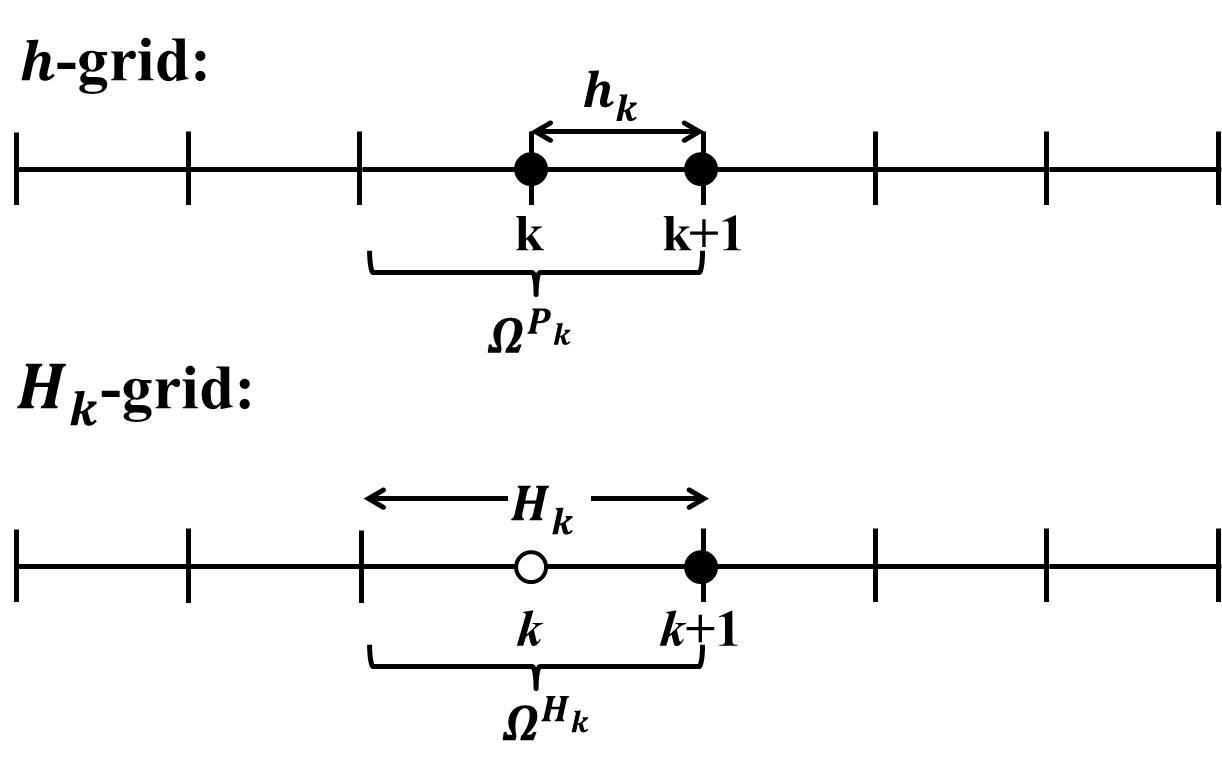
\includegraphics[width=0.45\textwidth]{figures/Setup/localization_grid.pdf}
\caption{1-D schematic of the $h$- and $H$-level grids for local VGI}
\label{fig:vgi_grid}
\end{figure}

The local VGI procedure then uses the
$H_k$-grids with the $h$-grid to compute the model
parameter at every node $k$ in the $h$-grid.
By setting $\bm{W}^h = \bm{W}^{H_k}$,
since $\bm{\mathcal{V}}^{H_k} \subset \bm{\mathcal{V}}^h \subset \bm{\mathcal{V}}$,
we get (for details see Ref.~\cite{bib:tran2017b}).

\begin{equation}
\label{eq:vgil}
\begin{split}
 M_{comb}(\bm{W}^{H_k},\bm{U}^h; C^k_S, h_k) - M_{comb}(\bm{W}^{H_k},\bm{U}^{H_k}; C^k_S, {H_k})  = \\
  -(B(\bm{W}^{H_k},\bm{U}^h)- B(\bm{W}^{H_k},\bm{U}^{H_k}))
\end{split}
\end{equation}

We recognize that determining $\bm{U}^{H_k}$ for each interior node $k$ involves a grid-level
computation or projection (operations which involve looping over the elements of the $H_k$-grid). This is prohibitive and therefore, a surrogate is considered.
$\bm{U}^{H_k}$ is approximated within the macro element
using a volume-weighted average of $\bm{U}^h$ while outside
of the macro element the solution is assumed to be the same between the two grid levels.
This assumption further bypasses a grid-level computation. This assumption arises from the requirement on the variational multiscale (VMS) method to provide a localization at the element level and the desire to yield nodal exactness at element corners\cite{bib:hughes3}.
This leads to
$\bm{U}^{H_k} \approx \widetilde{\bm{U}}^{H_k}|_{\Omega^{H_k}} = \aHk(\bm{U}^h)$, where
$\aHk$ is the local averaging operator defined below.

\begin{equation}
\label{eq:avg}
\aHk (f^h) = \frac{1}{|\Omega^{P_k}|}\int\limits_{\Omega^h_e\in\Omega^{P_k}} f^h d\Omega^h_e
\end{equation}
\noindent where $|\Omega^{P_k}|$ is the volume of the local patch
and $\Omega^h_e$ indicates an element in the $h$-grid.

This choice is only feasible when the spatial derivatives exist on the weight function.
In addition, instead of using $\widetilde{\bm{U}}^{H_k}$ to compute $\bm{S}^{H_k}$, $\bm{S}^{H_k}$ is also approximated within the macro element as $\widetilde{\bm{S}}^{H_k}|_{\Omega^{H_k}} \approx \aHk(\bm{S}^h)$.
Furthermore, among all of the terms in Equation~\eqref{eq:vgil} 
not involving the unknown model parameter, the non-linear convective 
term is found to be dominating\cite{bib:tran2017b}. We note that this assumption holds 
exactly in a spectral setting where all the bilinear terms cancel out 
between the $H$- and $h$-level grids due to the $L_2$ orthogonality of 
spectral modes\cite{bib:oberai2005_2}. 
The local VGI simplifies to

\begin{equation}
	\label{eq:vgilb}
\begin{split}
% M_{smag}(\bm{W}^{H_k},\bm{U}^{h}; C_S^k, h_k)_{\Omega^{P_k}} - M_{smag}(&\bm{W}^{H_k},\widetilde{\bm{U}}^{H_k} ; C_S^k, H_k)_{\Omega^{H_k}}\\
% \approx -(B_2(\bm{W}^{H_k},\bm{U}^{h})_{\Omega^{P_k}} - B_2(\bm{W}^{H_k},\widetilde{\bm{U}}^{H_k})_{\Omega^{H_k}} )
-(B_2(\bm{W}^{H_k},\bm{U}^{h})_{\Omega^{P_k}} - B_2(\bm{W}^{H_k},\widetilde{\bm{U}}^{H_k})_{\Omega^{H_k}} \\
 M_{smag}(\bm{W}^{H_k},\bm{U}^{h}; C_S^k, h_k)_{\Omega^{P_k}} - M_{smag}(&\bm{W}^{H_k},\widetilde{\bm{U}}^{H_k} ; C_S^k, H_k)_{\Omega^{H_k}}
\end{split}
\end{equation}

Now an appropriate choice for $\bm{W}^{H_k} \in \bm{\mathcal{V}}^{H_k}$ must be made. 
In a 1D setting, we select
$\bm{W}^{H_k}=[w^{H_k}_i,0]^T$ with $w^{H_k}_i$
such that it is linear along a spatial direction within the
macro element and is constant or flat outside.
Within the macro element, $w^{H_k}_i$ is selected such that

\begin{equation}
\label{eq:wij}
w^{H_k}_{i,j} = \frac{1}{|\Omega^{H_k}|}
\end{equation}

\noindent where $|\Omega^{H_k}|$ is the volume of the
element. 
% In Figure \ref{fig:vgilocal}, $w^{H_k}_i$ is shown in 1D (in the $x_j$ direction).
% \begin{figure}[H]
% \centering
% \includegraphics[width=0.75\textwidth]{figures/localization.jpg}
% \caption{A 1D schematic of $w^{H_k}_i$ for the local VGI procedure}
% \label{fig:vgilocal}
% \end{figure}
This choice of $\bm{W}^{H_k}$
is feasible in a multi-D setting and on an
unstructured mesh consisting elements of mixed topology,
however, a larger patch must be considered. An extra layer
of elements is needed around the macro element to attain a constant value
in the outside region. This extra layer acts as a buffer region.
This choice is made due to its ease of implementation.
For more details see Refs.~\cite{bib:tran2017b}.


\subsection{Local VGI Computation}
\label{sec:VGIComp}

At this point we drop the subscript $k$ in $H_k$ and $P_k$ and superscript
$k$ in $C_S^k$ for brevity and only use it when necessary.
The residual of the local VGI is defined as

\begin{equation}
\label{eq:vgilres}
\epsilon_{ij} = L_{ij} - 2 (C_S h)^2 M_{ij}
\end{equation}
\noindent where
\begin{equation}
\label{eq:lij}
L_{ij} = \left(\left(\frac{1}{|\Omega^H|}, u^h_i u^h_j\right)_{\Omega^P} - \left(\frac{1}{|\Omega^H|}, \widetilde{u}^H_i \widetilde{u}^H_j\right)_{\Omega^H} \right)
\end{equation}
\begin{equation}
\label{eq:mij}
M_{ij} = \left(\left(\frac{1}{|\Omega^H|}, |S^h| S^h_{ij}\right)_{\Omega^P} - \left(\frac{H}{h}\right)^2\left(\frac{1}{|\Omega^H|}, |\widetilde{S}^H| \widetilde{S}^H_{ij}\right)_{\Omega^H} \right)
\end{equation}

The least squares method is applied to determine the model parameter as follows
\begin{equation}
\label{eq:vgi_cs}
(C_S h)^2 = \frac{1}{2}\frac{L_{ij}M_{ij}}{M_{ij}M_{ij}}
\end{equation}

Since the local VGI procedure often leads to negative values
for $(C_S h)^2$, an averaging scheme is employed to avoid this issue.
Specifically, Lagrangian averaging 
is applied\cite{bib:meneveau96}.
To do so, two additional advection-relaxation scalar equations are solved.
These are shown in Equations~\eqref{eq:ILM} and~\eqref{eq:IMM}.
The scalars $I_{LM}$ and $I_{MM}$ in these equations are the
Lagrangian-averaged counterparts of
$L_{ij} M_{ij}$ and $M_{ij} M_{ij}$, respectively.

\begin{equation}
\label{eq:ILM}
  I_{LM,t} + (u_j - u^m_j) I_{LM,j} = \frac{1}{T} (L_{ij}M_{ij} - I_{LM})
\end{equation}

\begin{equation}
\label{eq:IMM}
  I_{MM,t}+ (u_j - u^m_j) I_{MM,j} = \frac{1}{T} (M_{ij}M_{ij} - I_{MM})
\end{equation}

\noindent where $T$ is the timescale over which averaging is applied.
Additionally, a local volume-weighted averaging
is also applied separately to the numerator and denominator
of Equation~\eqref{eq:vgi_cs} as follows

\begin{equation}
\label{eq:CS_LDS}
  (C_S h)^2 = \frac{1}{2}\frac{\aH(I_{LM})}{\aH(I_{MM})}
\end{equation}

\noindent where, as before, $\aH$ represents a local averaging operator.
This is equivalent to averaging over local pathtubes\cite{bib:tran2016,bib:tran2017b} and maintains the utility of the local VGI.



%%% Local Variables: 
%%% mode: latex
%%% TeX-master: t
%%% End: 
 % chapter 2
\label{chap:num_disc}

\chapter{VMS-based Error Estimator}

\label{chapter:APEE} %a posteriori error estimator

%TODO: explain bar and h equivalance for VMS-based coarse scale

In this work, we focus on controlling the spatial discretization error through an \textit{a posteriori} error estimate.
Ideally, \textit{a posteriori} error estimate must provide pointwise the exact error, $e^{exact}=u-u^h$, where $u$ is the exact solution and $u^h$ is the numerical approximation $u$, since knowing how the error varies over space allows us to better choose our spatial discretization. 
Of course, knowledge of the exact error implies knowledge of the true solution rendering the simulation pointless.
Therefore, we employ an approximate error estimate $\apee$ measured in some norm of interest such as the $L^2$ norm, $\HOne$ norm, or $\HOne$ semi-norm.
We would like that the the error estimate has a local representation over an element $k$ and bounds (from above) the exact error.

%The local error estimate property provides a means of motivating adaptive methods and the upper-bound property provides safety against underestimating the global error. 
%An additional desired, but signficantly stronger, property would be to have the local error estimate bound the local true error.
%To measure the performance of an error estimate, it is common practice to look at the global effectivity index, $\eta$, or simply effectivity

%\begin{equation}
%%\eta = \frac{\apee}{||u-u^h||_{*}}
%\eta = \frac{\apee}{||e||_{*}^{exact}}
%\end{equation}

%\noindent which is the ratio between the estimated error and the exact error.
%Note that a local effectivity can also be defined on the element-level.

Many estimators, both explicit and implicit, have been developed and studied in the literature (e.g. see books by Ainsworth and Oden \cite{ainsworth2011book}, Verf\"urth \cite{verfurth2013posteriori}).
%and convection-diffusion systems (reviewed by John \cite{john2000numerical} and Verfurth \cite{verfurth2005robust}).
More recently, progress has been made in obtaining reliable explicit error estimates for the Navier-Stokes equations through the variational multi-scale approach (e.g. Hauke, Fuster, and Lizarraga \cite{hauke2015variational}).
%Although even in the context of convection-diffusion systems, John \cite{john2000numerical} finds that there is no optimal approach for all situations.
We employ the VMS-based error estimator since the VMS framework is currently used for LES and it is computationally inexpensive.

%In this work, we develop an explicit error estimator for the Navier-Stokes equations similar to that found in Hauke \textit{et al} \cite{hauke2015variational} in that we take advantage of the variational multiscale approach (VMS), which yield local error estimates in the norm of our choice. 
%A primary difference is in the norm which we choose to measure the error - $\HOne$ seminorm vs. $L^2$ or $L^1$.
We first review the general formulation of the VMS approach.
We then discuss the error estimator based on the VMS approach for a model 1D advection-diffusion problem followed by how it can be extended to a multi-dimensional setting.
We then extend the VMS-based error estimator to the Navier-Stokes equations and periodic problems of interest.

\section{General Formulation}
\label{sec:VMS_form}

%What is VMS?

The VMS paradigm relies on the idea of decomposing spaces of interest into coarse-scale and fine-scale subspaces.
The coarse-scale space represents our choice of spatial discretization and is therefore finite dimensional, whereas the fine-scale space encompasses the remainder of the space that our discretization cannot represent and is therefore infinite dimensional.
More importantly, the fine-scale space is necessarily a representation of the spatial discretization error for the solution space.

Let us specifically consider the trial and weighting spaces for some model finite element problem as $\mathcal{S}$ and $\mathcal{W}$, respectively.
%Let $\mathcal{S}^h$ or $\bar{\mathcal{S}}$ be a subset of $\mathcal{S}$ and let $\Projector: \mathcal{S} \rightarrow \mathcal{S}^h$ or $\bar{\mathcal{S}}$ be a linear projector such that $\Projector u = u^h = \bar{u}$ where $u \in \mathcal{S}$, $u^h=\bar{u} \in \mathcal{S}^h=\bar{\mathcal{S}}$, and $Range(\Projector)=\mathcal{S}^h=\bar{\mathcal{S}}$.
Let $\bar{\mathcal{S}}$ be a subset of $\mathcal{S}$ and let $\Projector: \mathcal{S} \rightarrow \bar{\mathcal{S}}$ be a linear projector such that $\Projector u = \bar{u}$ where $u \in \mathcal{S}$, $\bar{u} \in \bar{\mathcal{S}}$, and $Range(\Projector)=\bar{\mathcal{S}}$.
This naturally leads to the definition of a complementary space $\mathcal{S}' = Kernel(\Projector)$ and allows for the direct sum decomposition $\mathcal{S} = \bar{\mathcal{S}} \oplus \mathcal{S}'$ and $\mathcal{W}$ = $\bar{\mathcal{W}} \oplus \mathcal{W}'$, where $\bar{\mathcal{S}}$ and $\bar{\mathcal{W}}$ represent the coarse-scale subspaces and $\mathcal{S}'$ and $\mathcal{W}'$ represent the fine-scale subspaces. This is a similar decomposition to that used in XXX\ref{chapter_2} for LES to define the coarse- and fine-scale solutions: $u^h$ and $u'$, where the fine-scale solution contributes to the subgrid-scale model.
Here, the fine-scale solution is used to determine the element-level or local error. In the following, we use $\bar{u}$ for fine-scale quantities. In summary, $\bar{\mathcal{S}}$ is the same as $\mathcal{S}^h$ and $\bar{u}$ is the same as $u^h$. This equivalence applies for the coarse-scale weighting space as well. 
We use the $\bar{(\cdot)}$ notation for the coarse-scale quantities in this section to be consistent with the most prevalant literature on VMS-based error estimation (i.e., it is slightly different from the notation used previously).

Because of the direct-sum representation, we can also state that $u=\bar{u}+u'$ is a unique decomposition where $\bar{u} \in \bar{\mathcal{S}}$ and $u' \in \mathcal{S}'$ for any $u \in \mathcal{S}$.


Consider the usual statement of a homogeneous linear partial-differential equation with linear operator $\mathcal{L}$ and forcing function $f$

\begin{equation}
    \mathcal{L}(u) = f \qquad u|_{\Gamma} = 0
    \label{eq:modelProblem}
\end{equation} 

\noindent which yields the following finite element problem:
find $u \in \mathcal{S}$ such that

\begin{equation}
    B(w,u) = (w,f), \qquad \forall w \in \mathcal{W}
\end{equation} 

\noindent where $B(\cdot,\cdot)$ is a bilinear form stemming from integration by parts of Equation \ref{eq:modelProblem} and $(\cdot,\cdot)$ is the $L^2$ inner product.

Applying the scale decomposition and leveraging the direct-sum representation yields a coarse-scale problem and a fine-scale problem.

Find $\bar{u} \in \bar{\mathcal{S}}$ such that
\begin{equation}
    B(\bar{w},\bar{u}) + B(\bar{w},u') = B(\bar{w},\bar{u}) + (\mathcal{L}^{*}\bar{w},u') = (\bar{w},f), \qquad \forall \bar{w} \in \bar{\mathcal{W}}
\end{equation} 

Find $u' \in \mathcal{S}'$ such that
\begin{equation}
    B(w',\bar{u}) + B(w',u') = (w',\mathcal{L}\bar{u}) + B(w',u') = (w',f), \qquad \forall w' \in \mathcal{W}'
    \label{eq:fineScale}
\end{equation}

The coarse-scale problem is coupled with the fine-scale problem through $u'$, which again is conveniently also a representation of the discretization error.
A further remark is that the coarse-scale problem has the form of a stabilized finite element method once a substitution for the form of $u'$ is made.
The fine-scale problem does afford a solution (see Hughes and Sangalli \cite{hughes2007variational}), where

\begin{equation}
    u'(y_i) = -\int_{\Omega} g'(x_i,y_i)(\mathcal{L}\bar{u}-f)(x_i) d\Omega
    \label{eq:uPrimeSoln}
\end{equation} 

\noindent where $g'(x_i,y_i)$ is the fine-scale Green's function with $x_i,y_j \in \Omega$, which is not known in general, except for certain cases - one of which is the 1D linear advection-diffusion equation.
Since the Navier-Stokes equations have advective and diffusive properties, we use the 1D linear advection-diffusion as a starting point to derive the a posteriori error estimator.

One final remark is that the form of the fine-scale Green's function is directly tied to the choice of projector $\Projector$.
This equivalently also means that the various choices of $\Projector$ leads to different unique pairings of $u$ and $u'$.
Hughes and Sangalli \cite{hughes2007variational} explored two options for the $\Projector$: $\Projector_{L^2}$ and $\Projector_{H^1}$, and found that for 1D advection-diffusion systems, the $\Projector_{H^1}$ led to a localization of $g'$ to single elements and led to an optimal solution for $\bar{u}$ in the $\HOne_0$-norm or $\HOne$-seminorm, making this choice a practical one.
The localization of $g'$ is ideal for constructing local error estimators.

\section{Formulation for 1D Advection-diffusion Equation}


The steady advection-diffusion equation with the strong form given by: find the scalar $\psi$ such that

\begin{equation}
\mathcal{L}(\psi) = a_i \psi_{,i} - \kappa \psi_{,ii} = f
\end{equation}

\noindent where $a_i$ is an advection vector, $\kappa$ is the diffusivity constant and $f$
is a forcing function.
We can define the corresponding spaces for the solution and weighting functions as usual

\begin{equation}
\label{eq:testspace}
\mathcal{S}_{\psi} = \{ v| v \in H^1(\Omega)^N, v = g \text{ on } \Gamma_g\} 
\end{equation}

\begin{equation}
\label{eq:Vweightspace}
\mathcal{W}_{\psi} = \{ w|w \in H^1(\Omega)^N, w = 0 \text{ on } \Gamma_g\}
\end{equation}

\noindent The corresponding weak form is given by: find $\psi \in \mathcal{S}_{\psi}$ such that

\begin{equation} 
\int_\Omega \left[ \wAD a_i \psi_{,i} + \kappa {\wAD}_{,i}\psi_{,i}\right] \, d\Omega- 
\int_{\Gamma_h} \kappa \wAD \psi_{,i} n_i\, d\Gamma_h = 
\int_\Omega \wAD f \, d\Omega, \qquad \forall \wAD \in \mathcal{W}_{\psi}
\label{eq:AD_model}
\end{equation}

Equation \ref{eq:uPrimeSoln} describes the relationship between the coarse-scale solution $\bar{\psi}$ and the discretization error.
The strong residual acts as a local source for error and the fine-scale Green's function distributes it over the spatial domain.
%Following the optimality approximation of $\bar{u}$ in the $\HOne$-sense, we consider only the $\HOne$-seminorm.
From Equation \ref{eq:uPrimeSoln}, we can define the $\HOne$-seminorm over an element

\begin{equation}
    |e^{\psi}_k|_* = |e^{\psi}_k|_{\HOne(\Omega^h_k)} = |\psi'_k|_{\HOne(\Omega^h_{k})}= |(\mathcal{R}(\bar{\psi}_k)| \norm{ \int_{\Omega^{h}_{k}} g_{,i}' d\Omega^h_{k}}_{L^2(\Omega^h_k)}
\end{equation}

\noindent where $\mathcal{R}(\bar{\psi})=\mathcal{L}(\bar{\psi})-f=\mathcal{L}(\psi^h)-f$ is constant for piecewise linear finite elements with piecewise constant input data and material properties.
We focus on the $\HOne$-seminorm in particular since we want to control the error in the gradients in the solution field.

For the 1D advection-diffusion equation, the fine-scale Green's function has an analytical form (see Hauke, Doweidar, and Miana \cite{hauke2006proper}) that is used to attain the following simplified form

\begin{align}
      \norm{\psi_k'}_{H^1(\Omega^h_k)} &= \nu^{err}_{k,1D} |\mathcal{R}(\bar{\psi}_k)| \sqrt{|\Omega^h_k|} \\
            &= \nu^{err}_{k,1D} \norm{\mathcal{R}(\bar{\psi}_k)}_{L^2(\Omega^h_k)}
      \label{eq:VMSerr1D}
\end{align}

%\noindent where $\nu^{err}_{e,1D} = \dfrac{1}{|a|} min \left( \sqrt{\Peh},\dfrac{\Peh}{\sqrt{3}} \right)$ and $\Peh = \frac{h_e |a|}{2\kappa}$ is the cell-Peclet number.
\noindent where $\nu^{err}_{k,1D} = \dfrac{1}{|a_i|} \sqrt{\Peh \text{coth}({\Peh})-1}$ and $\Peh = \frac{h_k |a_i|}{2\kappa}$ is the cell-Peclet number, and $h_k$ denotes a local mesh size.

Note that this is an explicit expression which does not require solving additional differential equations (local or global) like implicit error estimators.
This makes Equation \ref{eq:VMSerr1D} inexpensive to evaluate, although limited in scope to the one-dimensional case. The effectivity of the VMS based error estimator was tested for a series of cell Peclet numbers $Pe_h$ by Zhang \cite{zhang19} and showed that across all cases, the VMS error estimator provides the exact error in 1D. 
This is expected since the VMS theory in 1D linear, steady advection-diffusion case makes no assumptions or approximations.

\subsection{Generalization of VMS Error Estimator}

\subsubsection{Generalization to Multi-dimensional Cases}

The primary component of Equation \ref{eq:VMSerr1D} that is one-dimensional is the parameter $\nu^{err}_{e,1D}$ because it is not immediately obvious how to choose $h_k$, the element mesh size, for multi-dimensional anisotropic elements.
This problem is equivalent to the problem found when generalizing the 1D stabilization expressions that are used in stabilized finite element methods for advection-diffusion equations to multi-dimensional problems \cite{hughes1986newiii} and can therefore be addressed with a similar approach.
%The generalization procedure follows three steps:

%\begin{enumerate}
%    \item Find the asymptotes of the expression for the advective and diffusive limits
%    \item Combine the asymptotes to get the final form
%    \item Employ the element metric tensor $g_{ij}$ in each limit 
%\end{enumerate}

%The asymptotes for $\nu^{err}_{k,1D}$ in Equation \ref{eq:VMSerr1D} are $\sqrt{\dfrac{h_k/2}{{\kappa|a_i|}} }$ for the advective limit and $\dfrac{ h_k/2 } {{\kappa\sqrt{3}}}=\sqrt{ \dfrac{(h_k/2)^2} {3\kappa^2}  }$ for the diffusive limit.
%They can then be combined through the following expression

%\begin{equation}
%    \nu^{err}_{k,1D} \approx \dfrac{1}{\sqrt{\dfrac{\kappa|a_i|}{h_k/2} + \dfrac{3\kappa^2}{(h_k/2)^2} } }
%\end{equation}

For advective-diffusive systems, there are two element-sizes of interest - one corresponding to the direction of local advection and the other corresponding to diffusion.
This is reflected in the asymptotes for the exact expression for $\nu^{err}_{k,1D}$. %Equation \ref{eq:VMSerr1D}.
The magnitude of the local advection relative to the local mesh size $\dfrac{|a_i|}{h_k/2}$ can be represented with $\sqrt{a_i g_{ij} a_j}$ as $g_{ij} = \left(\dfrac{2}{h_k}\right)^2$ in 1D.
For the diffusive length-scale, the metric tensor intrinsically represents an average mesh size for an element so $g_{ij}g_{ij}$ provides a convenient choice.
This leads to the final generalized result for $\nu^{err}_k$

\begin{equation}
    \nu^{err}_{k} = \dfrac{1}{\sqrt{ \kappa\sqrt{a_i g_{ij} a_j} + 3\kappa^2\sqrt{g_{ij}g_{ij}}  }  }
\end{equation}

\noindent and the subsequent final form of the a posteriori error estimator

\begin{equation}
      |e^{\psi}_k|_{\HOne(\Omega^h_k)} = \seminorm{\psi'_k}_{H^1(\Omega^h_k)} \approx \nu^{err}_{k} \norm{\mathcal{R}(\bar{\psi}_k)}_{L^2(\Omega^h_k)}
      \label{eq:VMSerr}
\end{equation}

The effectivity of the VMS-based error estimator in 2D was tested by Zhang \cite{zhang19} for a 2D advection-diffusion problem. For this multi-dimensional case, it is reported that the error estimator does not exactly capture the true error. Instead, for a wide-range of $Pe_h$ the global effectivity was slightly greater than unity.   
For $Pe_h=100$, the effectivity was approximately 1.1, which indicates that the error estimator is slightly overestimating the true error.
Note that an effectivity above 1 implies a more conservative error estimator. 
For an advection-diffusion-reaction problem with a similar $Pe_h$, Ainsworth et al. \cite{ainsworth2013fully} reports an effectivity of $\mathcal{O}(50)$ using the equilibrated residual method, which suggests that the VMS-based error estimator performs well.

 


\label{sec:1D_AD}

\section{Application to the Navier-Stokes Equations}
\label{sec:VMS_NS}
As discussed previously, the Navier-Stokes equations possess advective and diffusive properties and extending the stabilization expressions from the 1D advection-diffusion to 3D Navier-Stokes have been effective in previous work.
We follow the same path for applying Equation \ref{eq:VMSerr} to each momentum component of the Navier-Stokes equations and arrive at the following

\begin{align}
    \seminorm{\bm{e}^{NS}}^2_{\HOne(\Omega^h)} &= \sum_{i}\seminorm{e^{NS}_i}^2_{\HOne(\Omega^h_k)} \\
    \seminorm{e^{NS}_i}_{\HOne(\Omega^h_k)} &= \seminorm{u_i'}_{\HOne(\Omega^h_k)} \approx \nu^{err,NS}_{k} \norm{\mathcal{R}^{NS}_i (\bar{u}_k)}_{L^2(\Omega^h_k)} \\
    \nu^{err,NS}_{k} &= \dfrac{1}{\sqrt{ \nu\sqrt{\bar{u}_i g_{ij} \bar{u}_j} + 3\nu^2\sqrt{g_{ij}g_{ij}}  }  } \\
    \label{eq:VMSerrNS}
\end{align} 

\noindent which uses the momentum residual $R^{NS}_i(\bar{u})=R^{NS}_i(u^h)$.

The discretization error resulting from the continuity equation is ignored since it is generally insignificant compared to the momentum discretization error.

\iffalse
One noticeable omission from the $\nu^{err}_e$ expression is any dependency on the time step, which is commonly found in stabilization expressions. 
As a reminder, the current form for the error-constant is derived from a steady-state advection-diffusion problem, and we are interested in the effectiveness of this current form.
Any extensions to the error-constant pave the way for future work.

This approach differs from previous work in that we use the $\HOne$-seminorm to measure the error whereas Hauke et al. \cite{hauke2008variational,hauke2015variational} focuses on the $L^2$ and $L^1$ norms. 
Moreover, we reach the form of the error constant through a direct extension of the 1D advection-diffusion setting to multidimensional settings which has not been done previously.
\fi



\section{Application to Periodic Flow Problems}
We are interested in applying the VMS-based error estimator to periodic problems in space and/or time. The specific problem of interest in this case is flow over a surging airfoil. In this case, an airfoil oscillates sinusoidally in a constant freestream and is also periodic in the spanwise direction. The mesh for this case is first generated as a 2D/in-plane mesh (i.e., on the front surface), and then extrusion is applied in the spanwise direction.

Currently, an adapted mesh is constructed for the entire surging cycle since we are interested in turbulent flows with resolution of fine-scale structures/fluctuations and adapting at different time steps over an oscillation cycle can be computationally expensive. Thus, the VMS-based error estimator is applied to multiple instances/phases over the surging cycle, and the maximum local/elemental error over the surging cycle is chosen. Similarly, for a spanwise extruded mesh, the maximum local/elemental error in the spanwise direction over the extruded-stack of elements is selected.
\label{sec:app_to_periodic}

\section{Mesh Adaptation Strategies}
We explore three different adaptation strategies for mesh adaptation based on the VMS-based estimated error as discussed below. 

\subsection{Zonal Adaptation}

%TODO: Show some schematics. Cylinder/airfoil flow. Simple schematics with 2/3 zones. 


The first strategy we employ is error estimator based zonal refinement/adaptation. 
In this strategy, we obtain the solution on an initial mesh for the problem at hand. The VMS-based error estimator is then applied to the solution corresponding to this mesh, and based on the estimated error, the mesh is refined by a specified factor in particular zones where relatively high error values are found. Estimated error for this adapted mesh is then calculated, and the mesh is again refined by the specified factor in zones of high error. This process is repeated till it is computationally feasible, or when mesh convergence is reached.
Note that for this adaptation strategy, coarsening can possibly be done for zones with relatively low error, but was not needed in this work. The flowchart for this strategy is illustrated in Figure \ref{fig:zonal_based_strat}.

\begin{figure}[H]
	\centering
	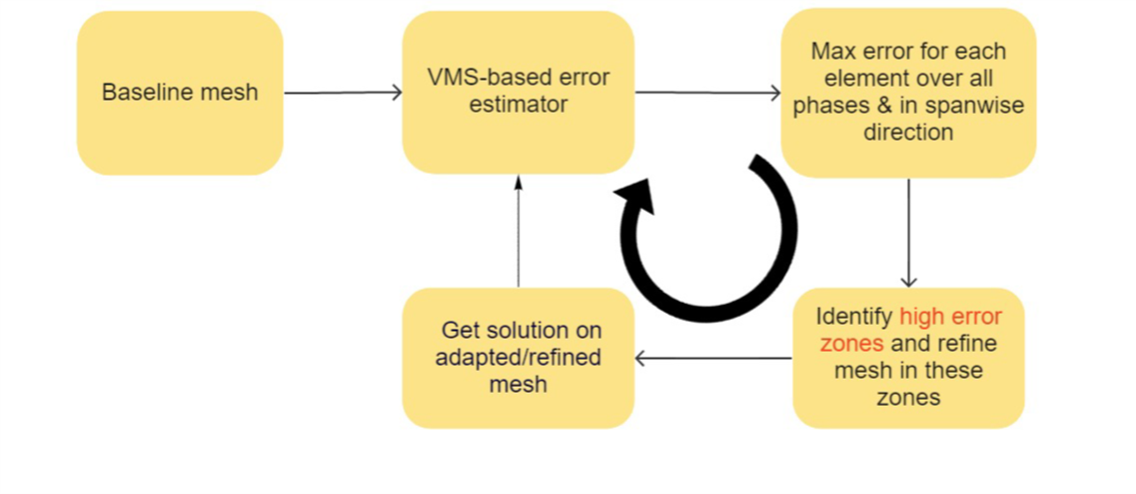
\includegraphics[width=1\textwidth]{figures/adapt_strat/zonal_based.png}
	\caption{Flowchart for zonal adaptation strategy}
	\label{fig:zonal_based_strat}
\end{figure}

For example, a sample of estimated error field in the case of flow over a surging airfoil is shown in Figure \ref{fig:zonal_based_strat_schematic}.
Note that maximum element-level error is obtained for all phases of the cycle and in spanwise direction.
Estimated error is higher in the wake region, as well as in the regions through which the leading edge vortex (LEV) traverses.
High error zones are identified in, and mesh in these zones is refined by a specified factor.

\begin{figure}[H]
	\centering
	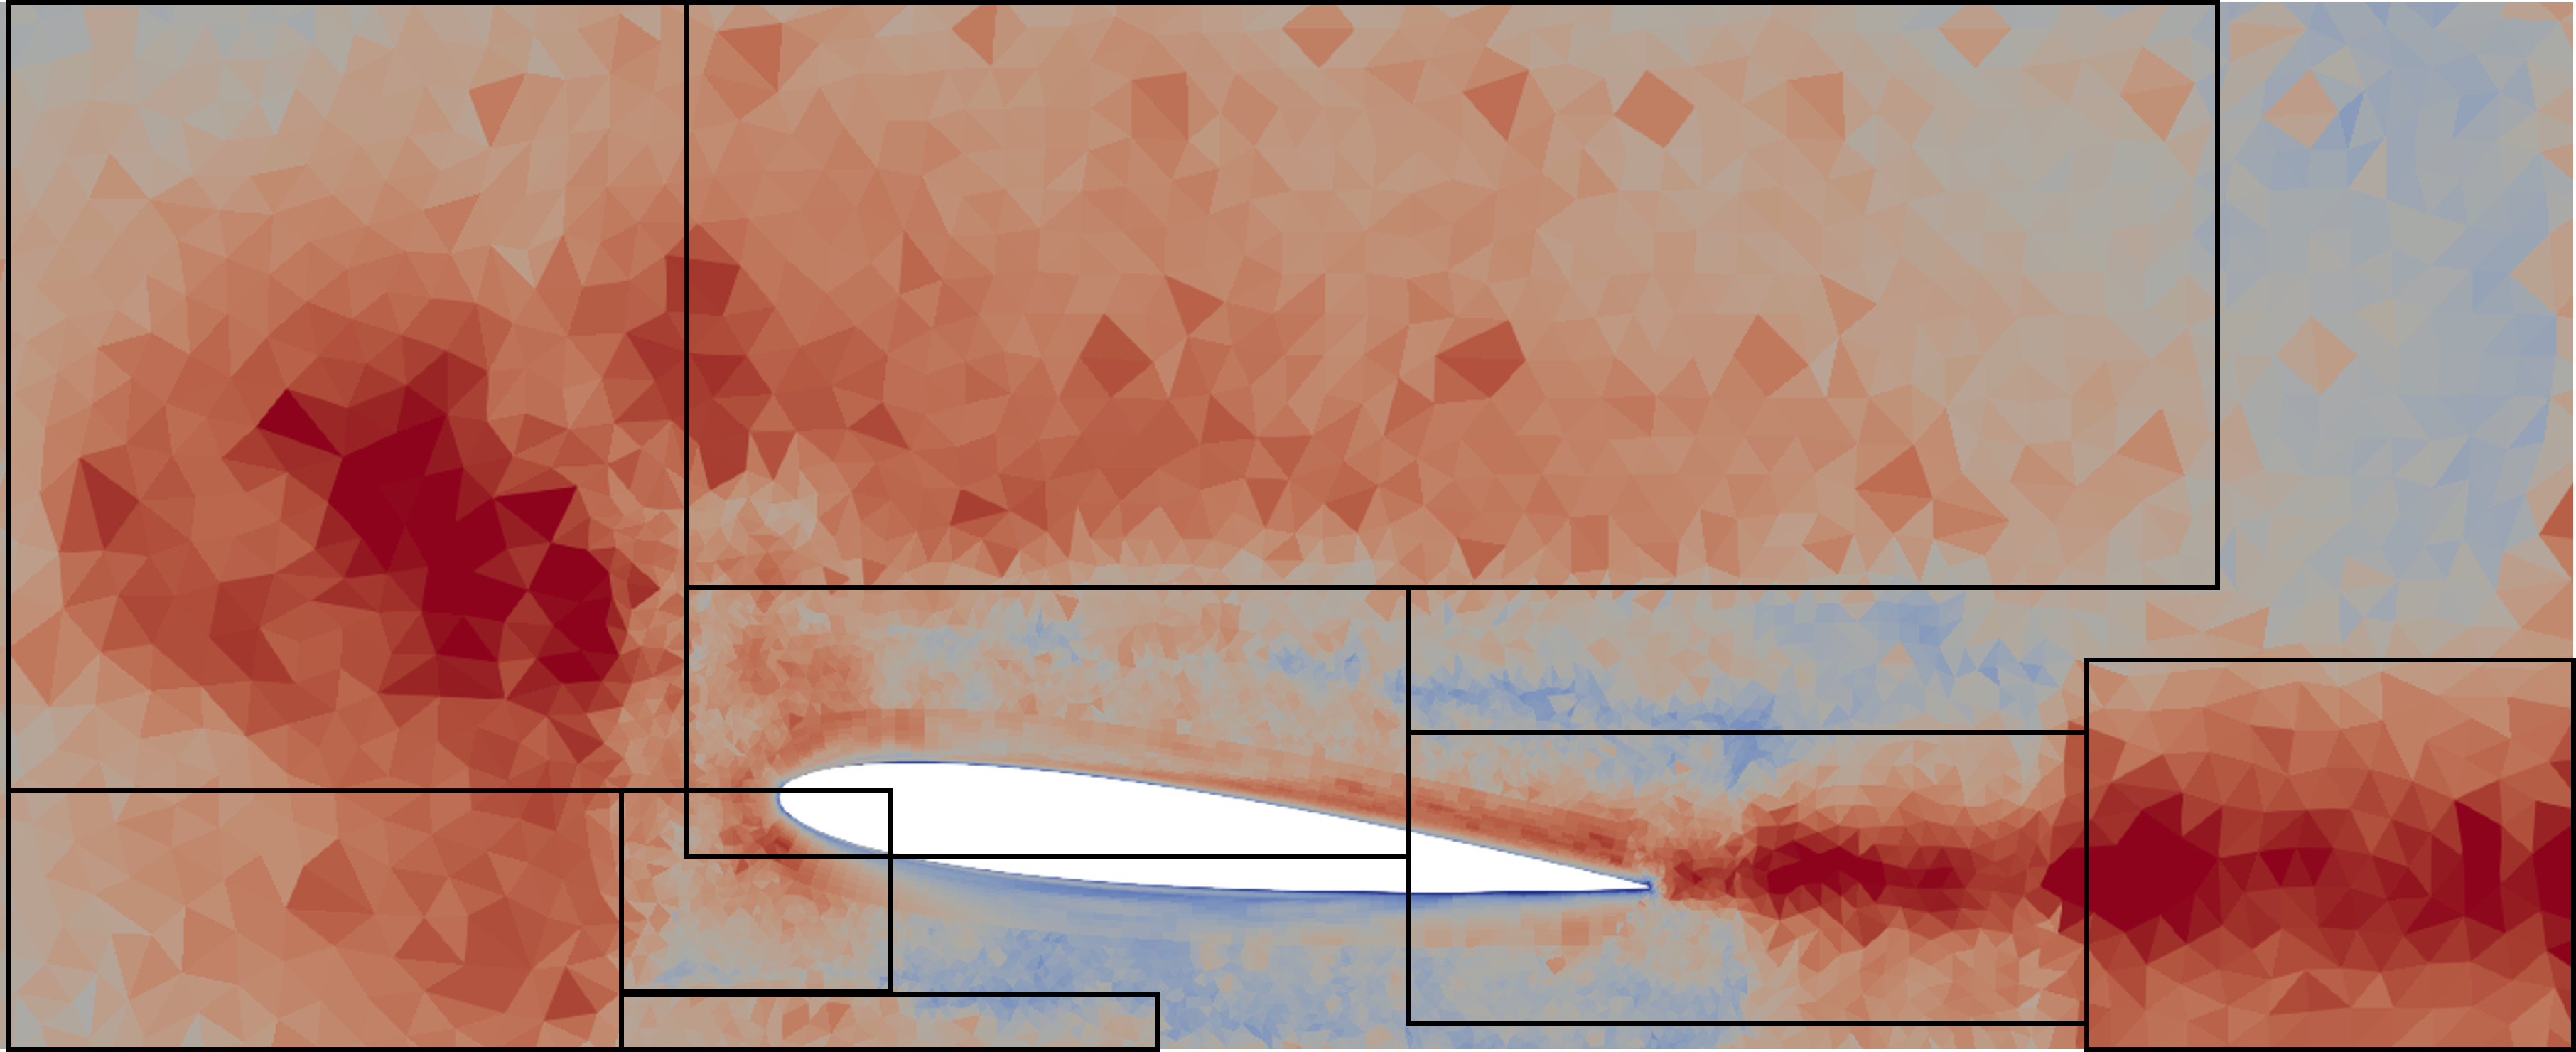
\includegraphics[width=0.75\textwidth]{figures/adapt_strat/zonal_based_schematic.png}
	\caption{Schematic of zonal refinement strategy}
	\label{fig:zonal_based_strat_schematic}
\end{figure}

\subsection{Nodal Size Field-based Adaptation}
\label{sec:sf_adapt}

The second strategy employs a fully automated mesh adaptation based on the VMS-based error estimator. In this strategy, the estimated error and a specified target error are used to compute the desired mesh size or resolution in a local fashion, i.e., at every mesh vertex. We refer to this as the nodal size field, and the mesh is refined or coarsened based on this nodal size field. 

In this adaptive strategy, the VMS-based error is calculated on the initial mesh. Based on the estimated error, a nodal size field is calculated using the following equation \cite{zhang19}

\begin{equation}
	\frac{e_k}{\tilde{e}_k} = \left(\frac{h_{old}}{h_{new}}\right)^{m+N/2} 
	\label{eq:diez}
\end{equation}

Here, $e_k$ is the measured local error (in the $\HOne$-seminorm) at an element $k$, $\tilde{e}_k$ is the local target error as specified by the user, $m$ is the polynomial order of the approximation space (i.e., $m=1$ for the linear finite elements used currently) , and $N$ is the number of spatial dimensions. $h_{old}$ is the current size of the element, and $h_{new}$ is the desired new mesh size.
This new mesh size at the element level is assembled at the node/vertex level to perform mesh adaptation.
The flowchart for this strategy is shown in Figure \ref{fig:size_based_strat}.

\begin{figure}[H]
	\centering
	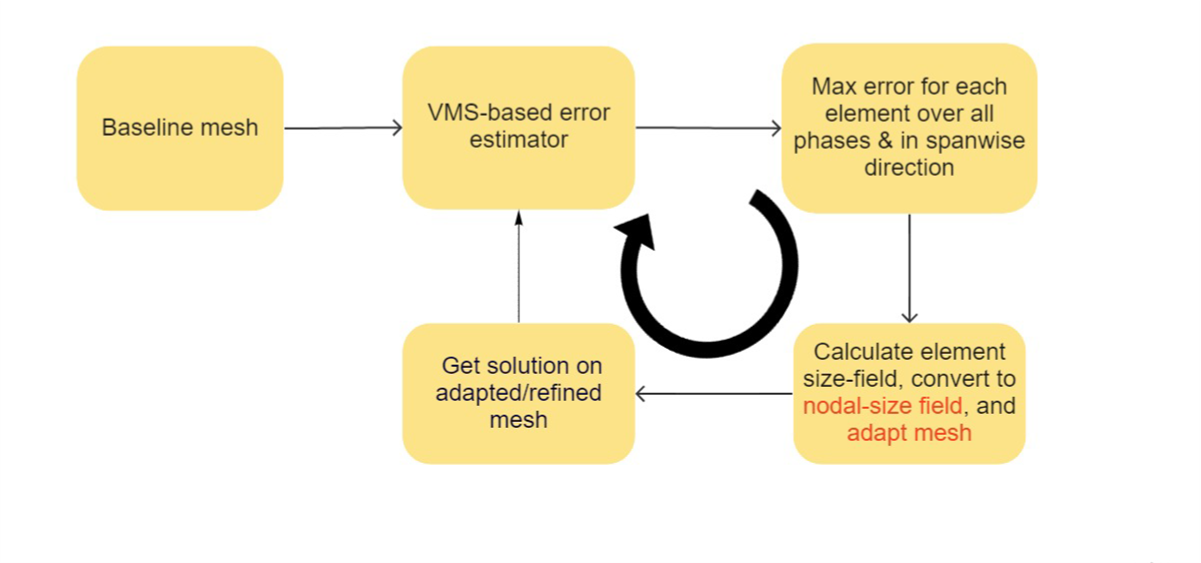
\includegraphics[width=1\textwidth]{figures/adapt_strat/size_based.png}
	\caption{Flowchart for nodal size field-based adaptation strategy}
	\label{fig:size_based_strat}
\end{figure}

\subsection{Feature-based Refinement/Adaptation}

The third strategy is to employ feature-based refinement/adaptation. 
This strategy allows for refinement around the dominant flow features and also along the path/trajectory of such features.
One of the primary flow features is the leading edge vortex (LEV) in the current problems of interest focused on surging airfoils. 
Figure \ref{fig:feature_based_strat_schematic} shows an example of the LEV path and size with respect to the airfoil. 
Mesh refinement is applied along this path as shown by the shaded region.


Two aspects are involved in this strategy: feature detection and tracking, and refinement/adaptation along the feature. These are discussed below.


	
\begin{figure}[H]
	\centering
	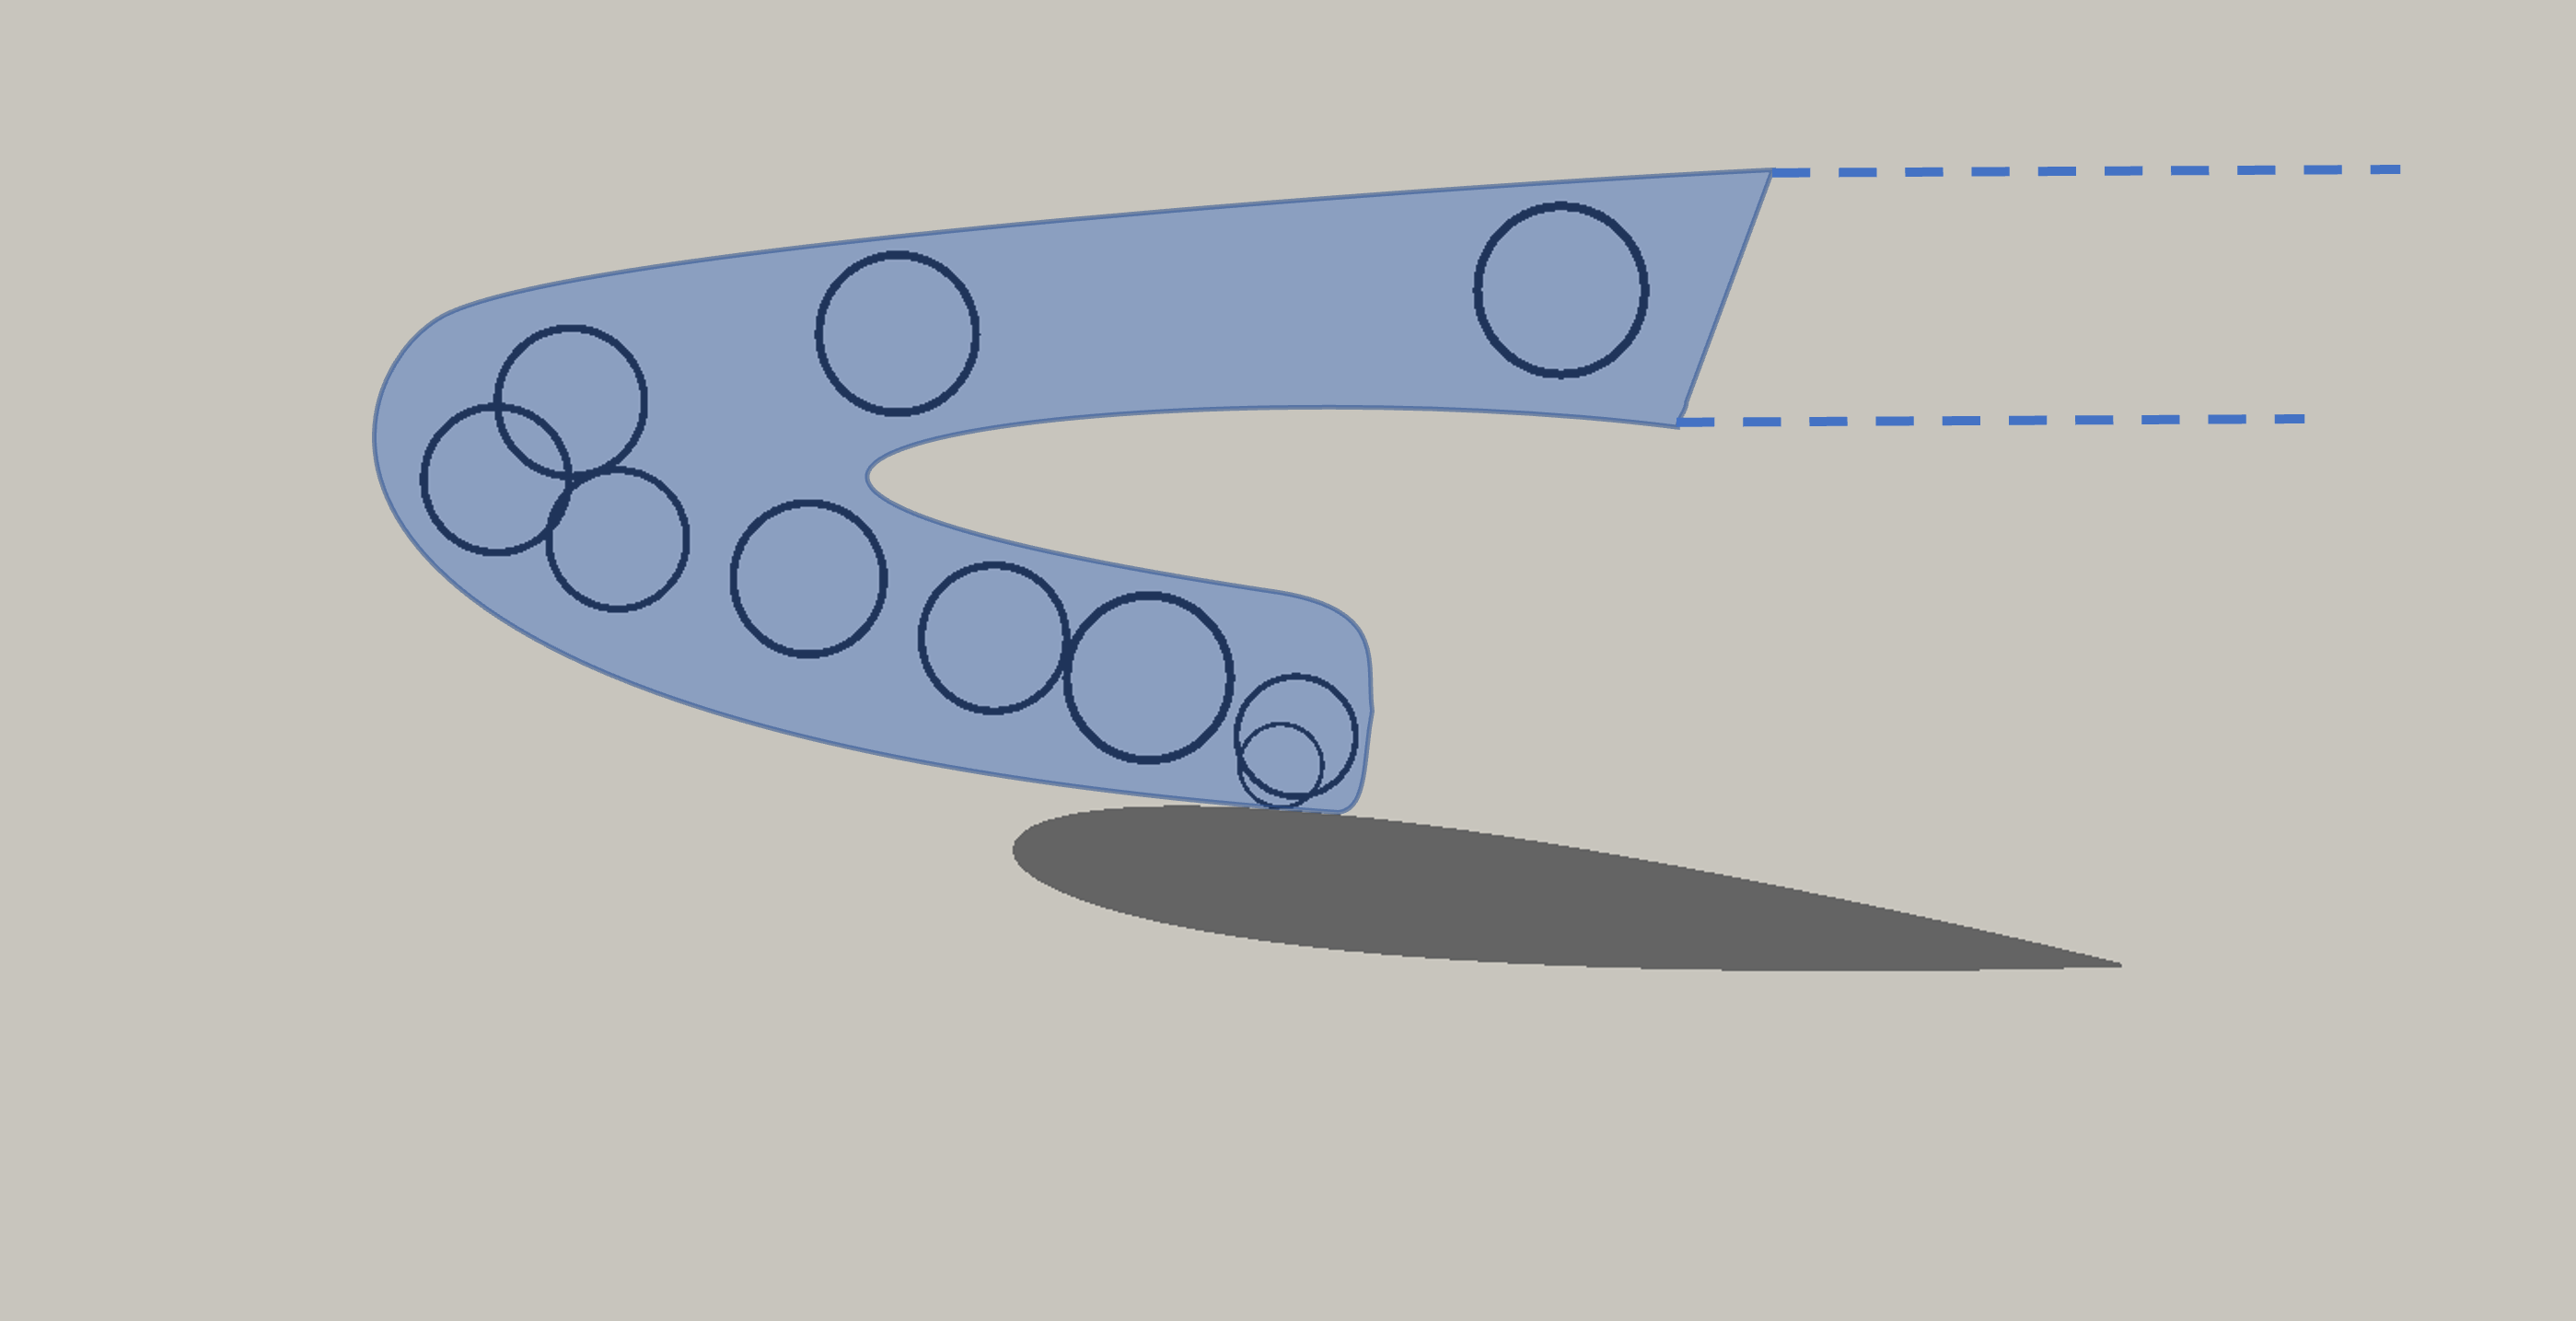
\includegraphics[width=0.75\textwidth]{figures/adapt_strat/feature_based_schematic.png}
	\caption{Schematic of feature-based refinement strategy}
	\label{fig:feature_based_strat_schematic}
\end{figure}

\subsubsection{LEV Detection and Tracking}
\label{sec:LEV_detect_track}

%TODO: Show pics and schematics from AIAA paper and presentations (LEV trace)

In this section, we quantify the evolution of the LEV based on its size and position.
In order to do so, phase- and spanwise-averaged data is obtained over multiple cycles.
Note that the LEV forms during the retreating portion of the surging cycle when the boundary layer separates and the separated shear layer rolls up into a vortex. Subsequently, this vortex separates/ejects from the airfoil, and advects with the background flow.
%For example, in Figure \ref{fig:LEV_tracking}, difference between the instantaneous and phase and span averaged vorticity is shown.
Thus, the phase of formation of the LEV is first detected and in subsequent phases the LEV is tracked.
Pressure and velocity data is analyzed to automatically detect the formation of the LEV.
In the retreating portion of the cycle, location with minimum pressure is determined starting at $\psi=180^\circ$.
The first phase at which the minimum pressure location is off the airfoil surface (i.e., away from the airfoil and into the flow) is tagged to be a potential phase for LEV formation.
At this potential phase, velocity profile is obtained over multiple lines passing through the minimum pressure location.
These are radial lines that are taken at an equispaced interval along the azimuth in the plane of the airfoil (note that the data is averaged in the spanwise direction).
These radial lines are shown in Figure \ref{fig:LEV_tracking2}.
Along these lines, at first a relative velocity is computed with respect to the velocity at the minimum pressure location.
Subsequently, normal component of the relative velocity is obtained (i.e., normal to each line), which is the azimuthal or tangential component in the polar coordinate system centered around the minimum pressure location.
The azimuthal component (of the relative velocity) is analyzed against the velocity profile of a Lamb-Oseen vortex.
It is noteworthy that the azimuthal component of the relative velocity along several radial lines at multiple phases in the surging cycle were visually analyzed for different cases and found to fit the Lamb-Oseen vortex model fairly well.

The trace of the LEV is then obtained by applying this process over multiple phases in the surging cycle, which can be used to quantify LEV evolution and to apply feature-based adaptation (as shown above in Figure \ref{fig:feature_based_strat_schematic}).

\begin{figure}[H]
	\begin{subfigure}{0.5\textwidth}
		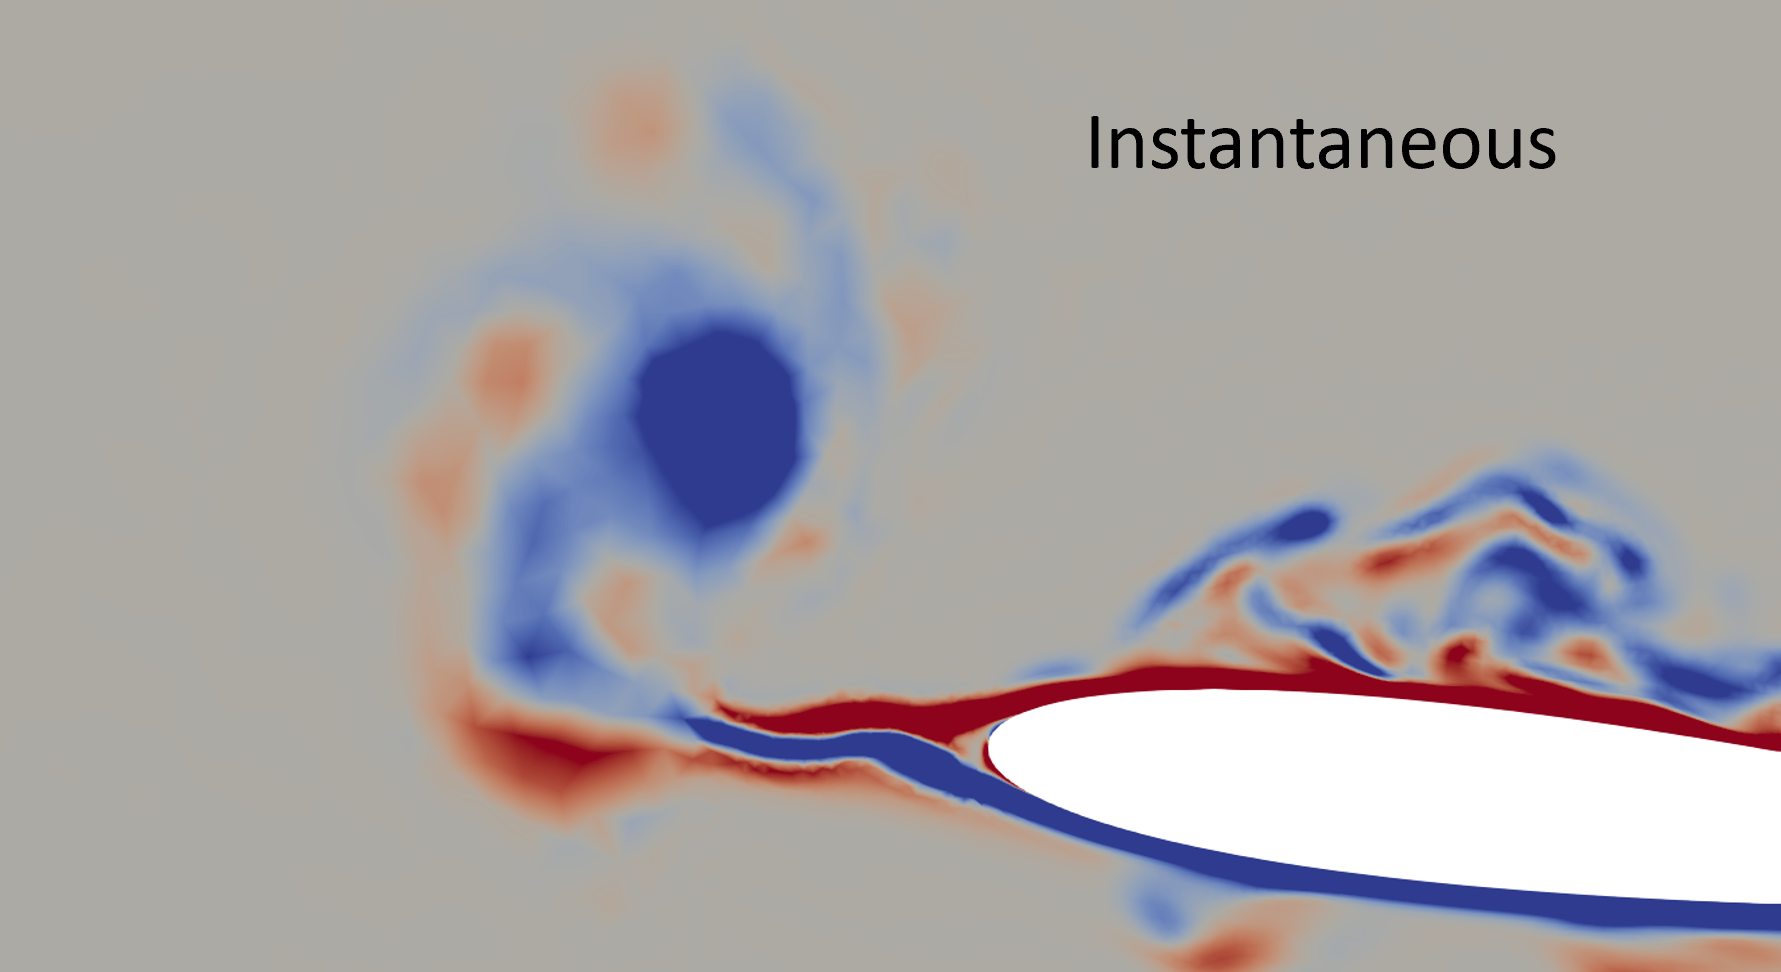
\includegraphics[width=1\textwidth]{figures/adapt_strat/LEV_tracking1.png}
		\caption{Instantaneous LEV}
		\label{fig:LEV_tracking1}
	\end{subfigure}
	\begin{subfigure}{0.51\textwidth}
	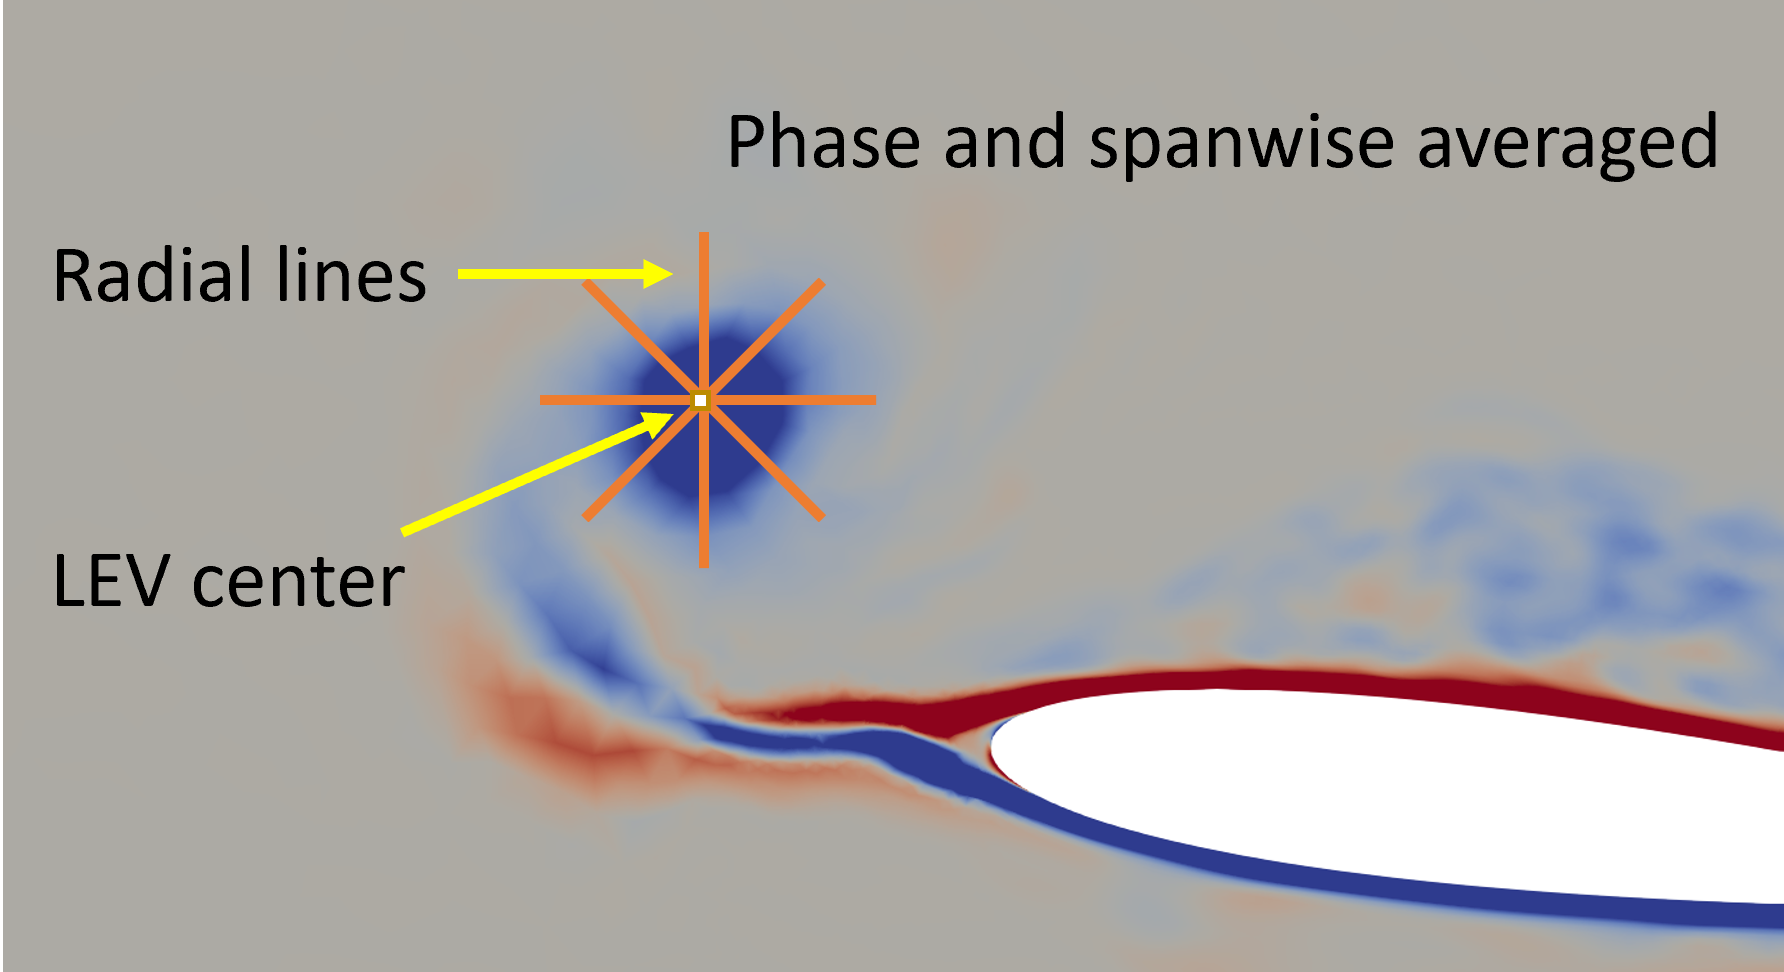
\includegraphics[width=1\textwidth]{figures/adapt_strat/LEV_tracking2.png}
	\caption{Averaged LEV}
	\label{fig:LEV_tracking2}
	\end{subfigure}

	\centering
	\begin{subfigure}{0.5\textwidth}
	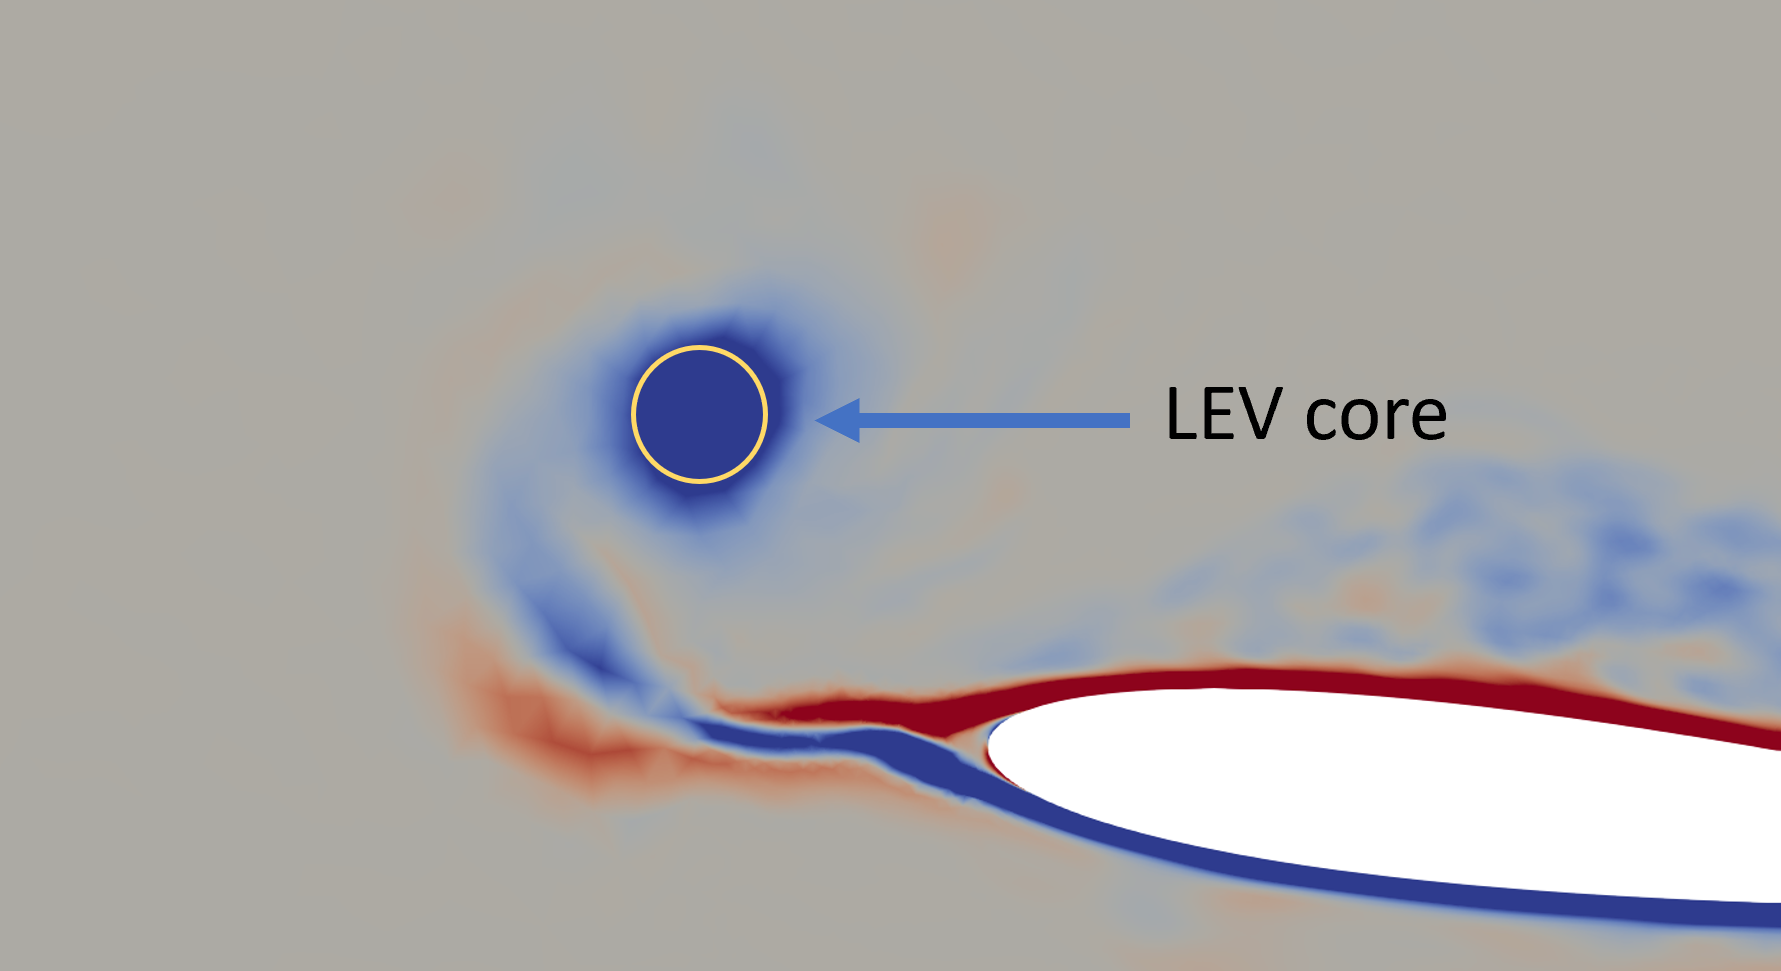
\includegraphics[width=1\textwidth]{figures/adapt_strat/LEV_tracking3.png}
	\label{fig:LEV_tracking3}
    \caption{Averaged LEV with core radius}
\end{subfigure}
	
	\caption{Schematic of LEV quantification}
	\label{fig:LEV_tracking}
\end{figure}


\subsubsection{LEV-based Refinement/Adaptation}

For a given simulation, we can follow three steps: (i) get information on the approximate path and extent that a certain feature will follow, (ii) estimate the error along this path/region, and (iii) perform refinement/adaptation along this path.
For example, in the case of flow over surging airfoils, the path and size of LEV over a surging cycle is used to detect portions in the mesh where refinement is applied.
Similarly, other features such as trailing edge vortex (TEV) can also be targeted using such a feature-based refinement. The flowchart for this strategy is shown in Figure \ref{fig:feature_based_strat}.

\begin{figure}[H]
	\centering
	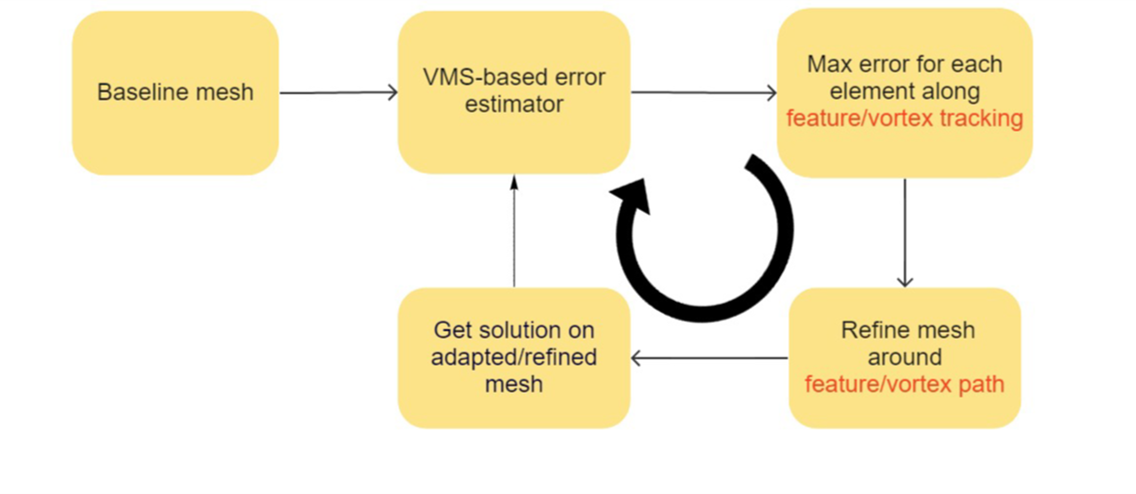
\includegraphics[width=1\textwidth]{figures/adapt_strat/feature_based.png}
	\caption{Flowchart for feature-based refinement strategy}
	\label{fig:feature_based_strat}
\end{figure}



\label{sec:adapt_strat_overview}
%\section{Non-dimensionalization of Error}

%One convenient aspect of the VMS approach to obtaining an error estimate is that the resulting units of the estimate are  



%%%xxx LATER Add a multi-D case (internal layer or boundary layer). Add a comment on Ainsworth 2013 paper with global effectivity order 60-100 for Pe of O(100).


\label{chap:vms_ee}

\chapter{LES of Flow Over Surging Airfoil}
\label{chapter:baseline_results}

In this chapter, we focus on LES of flow over a surging airfoil at different conditions. Problem setup as well as results including vortex detection and tracking are presented. A non-adapated mesh is used here to get familiar with the features of the current problem at different conditions, while results on the adapted meshes are presented in the next chapter.
% We also present active flow control cases in the form of active reflex camber. 

%\section{LES of Flow Over Surging Airfoil}
%\section{Adaptive LES of Flow Over Surging Airfoil}
%\section{LES of Flow Over Surging Airfoils including Active Reflex}


\section{Problem Setup}
\label{sec:problem_setup_baseline}

%TODO: Add U_rel velocity profile with t_tilde

A schematic of the problem setup is shown in Figure~\ref{fig:SetUpSketch}, where $U_\infty$ is the free-stream or mean velocity and $\alpha$ is the angle of attack.

\begin{figure}[H]
\centering
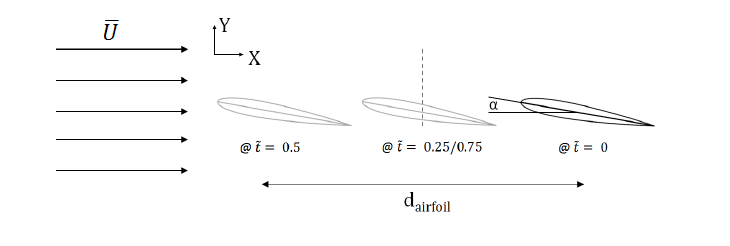
\includegraphics[width=0.8\textwidth]{figures/Setup/Setup.png}
\caption{Schematic of the surging airfoil problem}
\label{fig:SetUpSketch}
\end{figure}

The airfoil motion is set as follows
\begin{equation}
\label{eq:displacement}
  d_{airfoil} = A cos(2\pi f t) =  Acos(2\pi t/T) = Acos(2\pi\tilde{t})
\end{equation}

\noindent where $A$ is the amplitude and $T=1/f$ is the time period of the oscillation.
The variable $\tilde{t}$ is the fractional part in the oscillation cycle and is defined as $\tilde{t}=\{t/T\} = t/T - \lfloor t/T \rfloor$ (where $\lfloor \cdot \rfloor$ is the floor function).

The (non-dimensional) relative velocity is expressed as
\begin{equation}
\label{eq:relVelocity}
  \tilde{U}_{rel} = U_{rel}/U_\infty = 1 - U_{airfoil}/U_\infty = (1+\mu_{sect} sin(2\pi\tilde{t}))
\end{equation}
\noindent where $\mu_{sect}$ is the sectional advance ratio.
Note that for a sectional advance ratio above $1.0$ a negative relative velocity or a reversed flow condition is attained (e.g., at this radial section/location of the blade).
Under the reversed flow condition the relative flow is from the (geometric) trailing edge to the leading edge of the airfoil.

At $\tilde{t}$=0, with $\psi$=$0^\circ$ or $\psi$=$0^\circ$ (where, $\psi$ is the phase in the oscillation cycle and $\psi$ is the azimuthal position of the blade), the relative velocity is the free-stream velocity (i.e., $U_\infty$).
The same holds at $\tilde{t}$=0.5 or $\psi$=$180^\circ$.
At $\tilde{t}$=0.25 or $\psi$=$90^\circ$, the airfoil is at the maximum relative velocity and at $\tilde{t}$=0.75 or $\psi$=$270^\circ$ is at the minimum relative velocity.
Advancing part of the cycle is defined between $\tilde{t}$=0 or $\psi$=$0^\circ$ and $\tilde{t}$=0.5 or $\psi$=$180^\circ$, while retreating part is between $\tilde{t}$=0.5 or $\psi$=$180^\circ$ and $\tilde{t}$=1.0 or $\psi$=$360^\circ$ (or back to $\psi$=$0^\circ$).

The free-stream or mean Reynolds number is defined as: $Re=U_\infty C/\nu$, where $C$ is the chord.
The reduced frequency is defined as $k=\pi f C/U_\infty$ while the amplitude is related as $A = \frac{\mu_{sect} C}{2k}$.

\section{Summary of Cases}
\label{sec:baseline_case_summary}

In the current study, the reduced frequency is held fixed at $k$=0.133 while three Reynolds numbers of $Re$=40,000, 200,000 and 1,000,000 are considered together with two sectional advance ratios of $\mu_{sect}$=1.0 and 1.2, i.e., six cases are considered in total.
The angle of attack of the airfoil is set to 6$^\circ$.
Note that we considered the Reynolds number of $Re$=40,000 in a previous study~\cite{bib:kocher_scitech2017} that was selected in accordance with the experiments conducted in \cite{bib:granlund2016} where the airfoil was placed in a constant flow and oscillated in the streamwise direction.
The six cases are summarized in Table~\ref{table:summary_cases}.

\begin{table}[H]
\centering
\caption{Summary of cases}
\label{table:summary_cases}
\begin{tabular}{|l|c|c|c|c|}
\hline
Airfoil   & $\alpha$ & $k$ & $\mu_{sect}$ & $Re$ \\
\hline
\hline
NACA 0012 & 6$^\circ$ & $0.133$ & \{1.0, 1.2\} & \{40,000,\; 200,000,\; 1,000,000\} \\
\hline
\end{tabular}
\end{table}

The computational domain is set to be $100C$ x $50C$ x $0.2C$.
At the inlet, a constant free-stream velocity is applied
(note that the airfoil is moved sinusoidally in the streamwise direction).
No-slip condition is prescribed on the moving airfoil.
The top and bottom surfaces are set as slip walls.
Side surfaces in the spanwise direction (i.e., front and back surfaces) are imposed to be periodic.
A natural pressure condition is used at the outlet.
A second-order implicit time integration scheme, e.g., see \cite{bib:tran2017b}, is employed with about 1,440 steps in an oscillation cycle.

%TODO: give justification for this mesh ... typical LES resolution for a BL (based on highest Reynolds number in the surge cycle) ... but indicate no consideration taken for other flow features such as separation and LEV.
An unstructured hybrid/boundary layer mesh is used.
The mesh is comprised of hex and wedge elements which is generated by first generating a mesh on the front surface and by subsequently applying an extrusion in the spanwise direction. This (non-adapted) mesh is used for all cases listed above. Again, this is done to get familiar with the features of the current problem at different conditions, while mesh adaptivity is investigated in the next chapter. The non-adapted mesh is constructed by following recommended practices in terms of mesh resolution on the surface of the airfoil and around it, as discussed below.

Refinement zones are placed around the airfoil to resolve the flow structures of interest, see Figure \ref{fig:mesh} (where three refinement zones are noted).
In the finest refinement zone (Z1), mesh size is set to be $C/256$.
In the subsequent two zones (Z2 and Z3), it is set to be $C/128$ and $C/64$, respectively.
In the spanwise direction, 50 extruded elements are used.
A layered and graded mesh (with geometric growth) is used around the airfoil surface, see Figure \ref{fig:mesh2}.
The first layer height is set to be $\mathcal{O}(10^{-5} C)$ such that it is below 1 in wall units for all cases.
Similarly, mesh spacing on the airfoil surface in the streamwise and spanwise directions is set to be below 80 and 50 in wall units, respectively, for the XXX (which Reynolds number and which part of the cycle).
Overall the mesh contains about 6.2 million nodes and 10.8 million elements.

\begin{figure}[H]
\centering
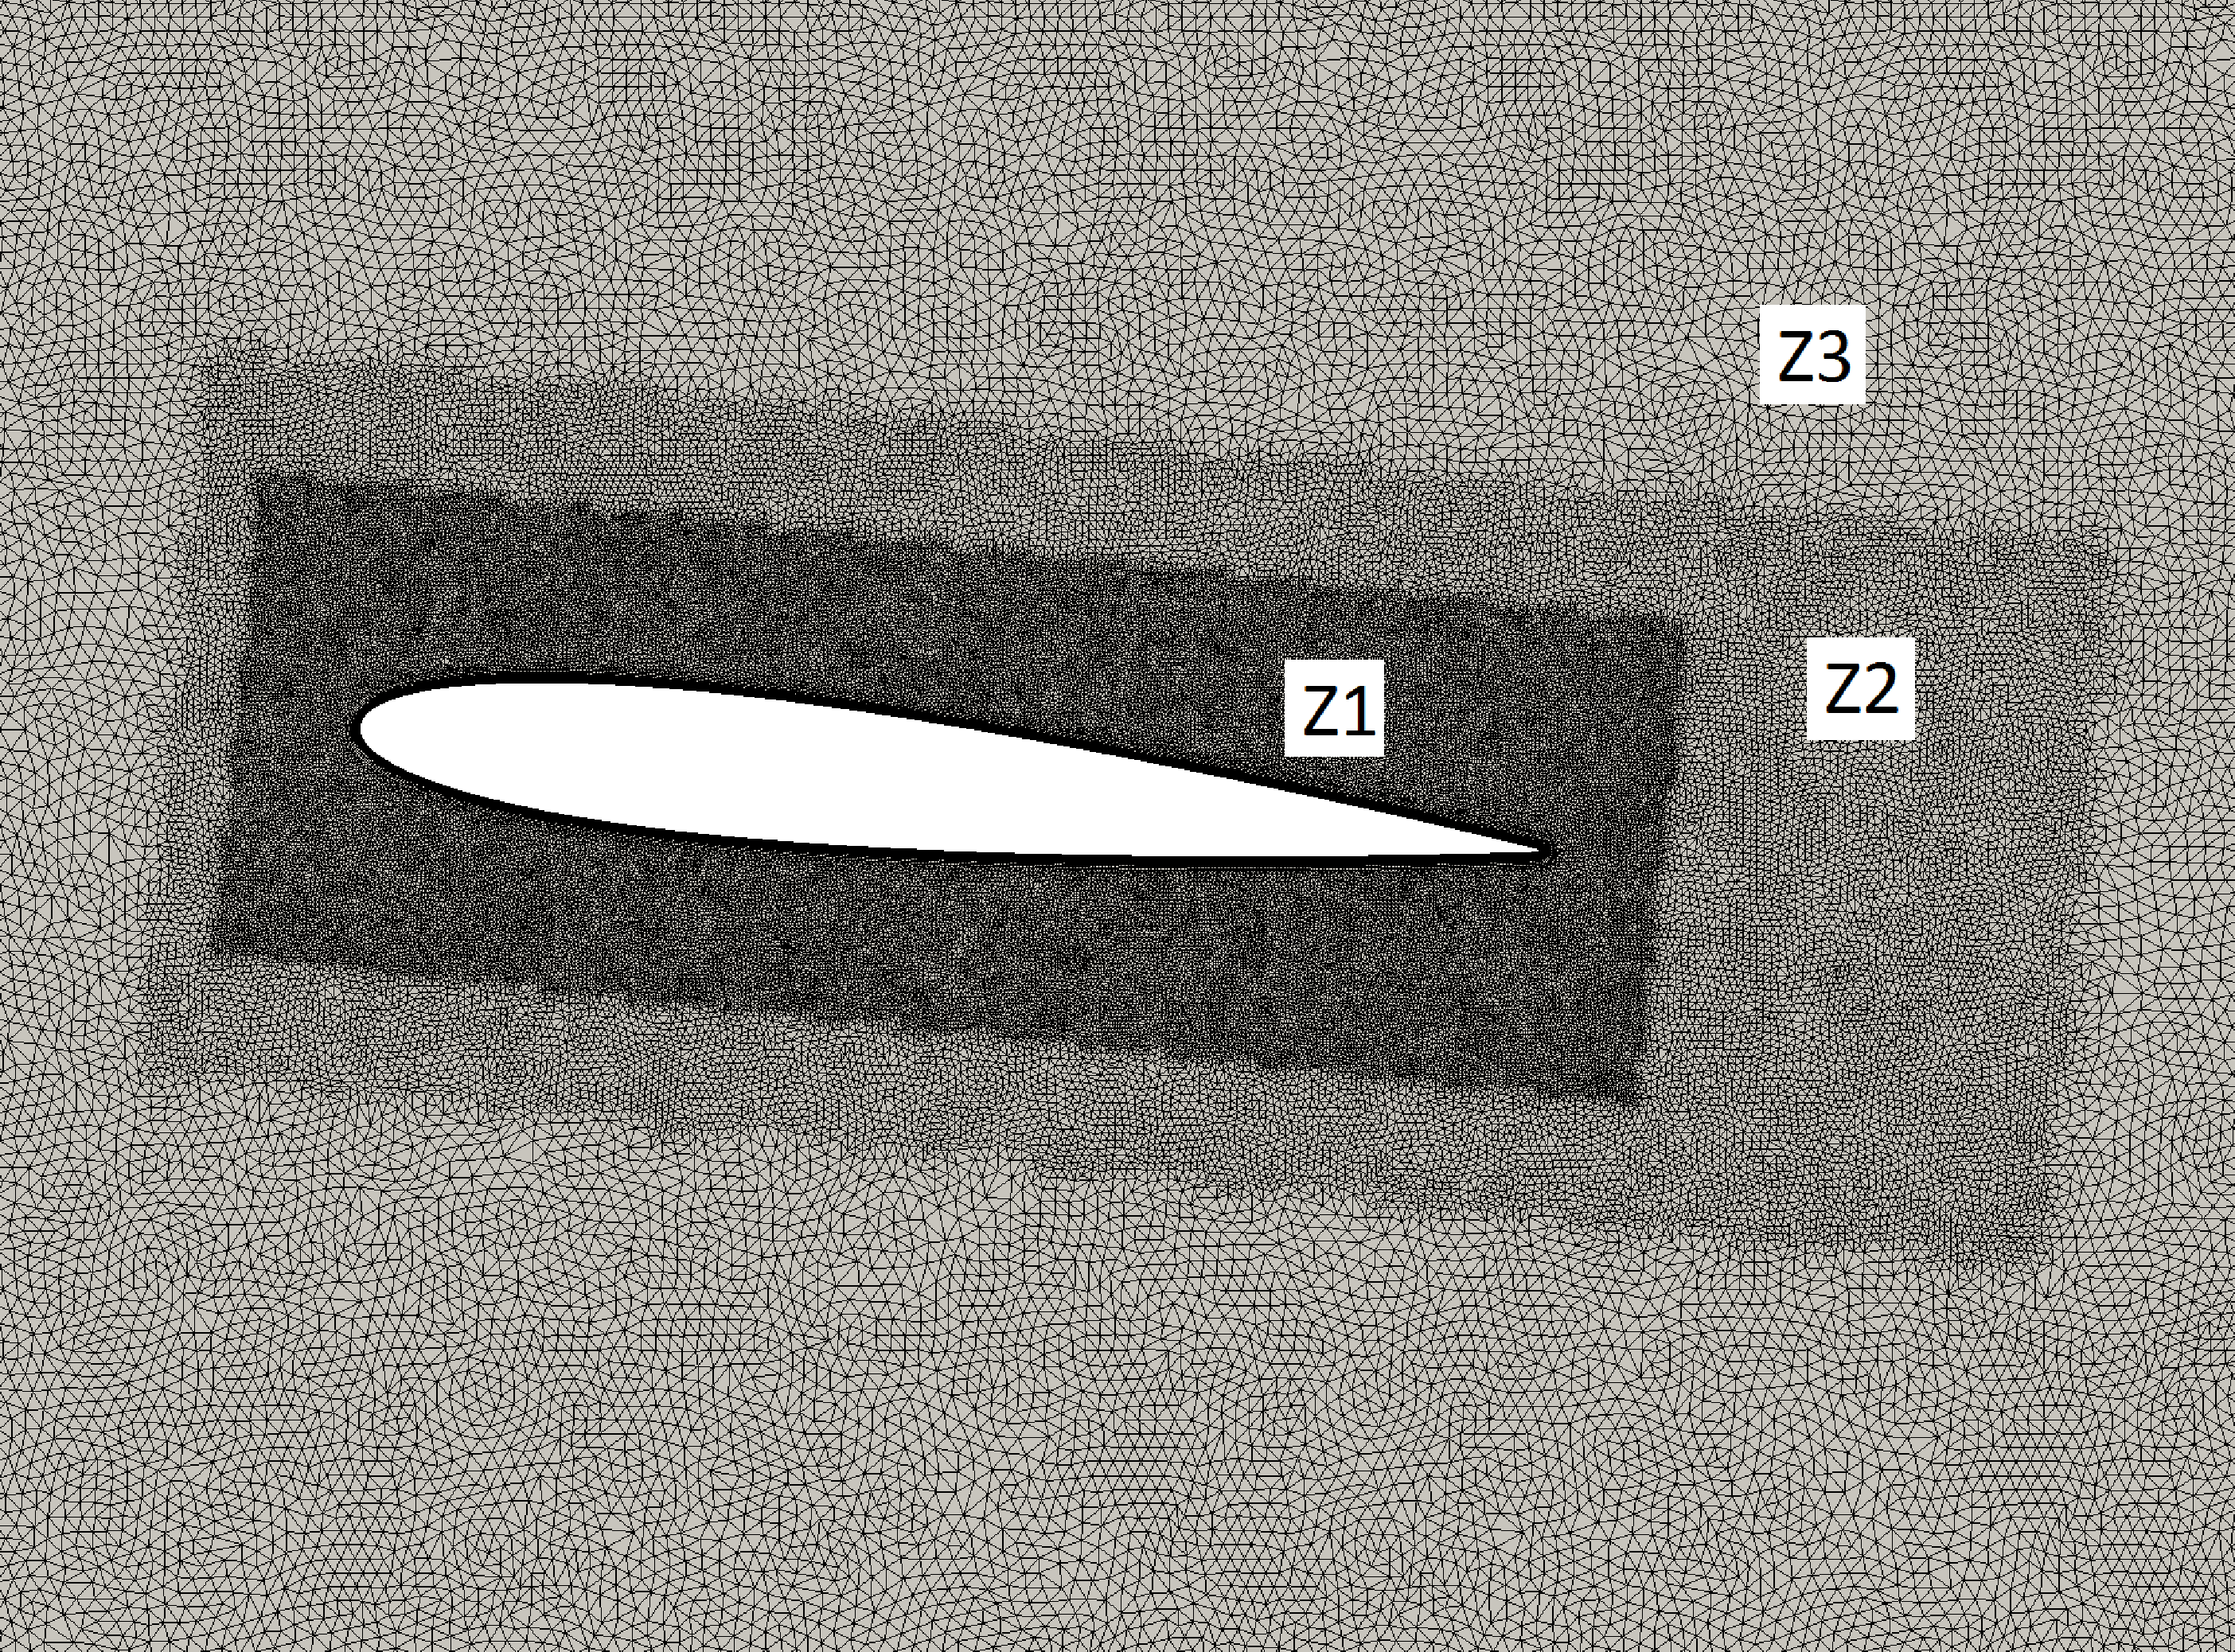
\includegraphics[width=0.7\textwidth]{figures/Setup/mesh_screenshot.pdf}
\caption{Mesh around the airfoil with refinement zones}
\label{fig:mesh}
\end{figure}

\begin{figure}[H]
\centering
\includegraphics[width=0.45\textwidth]{figures/Setup/mesh_LE.pdf}
\includegraphics[width=0.45\textwidth]{figures/Setup/mesh_TE.pdf}
\caption{Layered and graded mesh around the leading edge and trailing edge of the airfoil}
\label{fig:mesh2}
\end{figure}

\section{Results and Discussion}

\subsection{Force Response}

\begin{figure}[H]
	\begin{subfigure}{0.5\textwidth}
		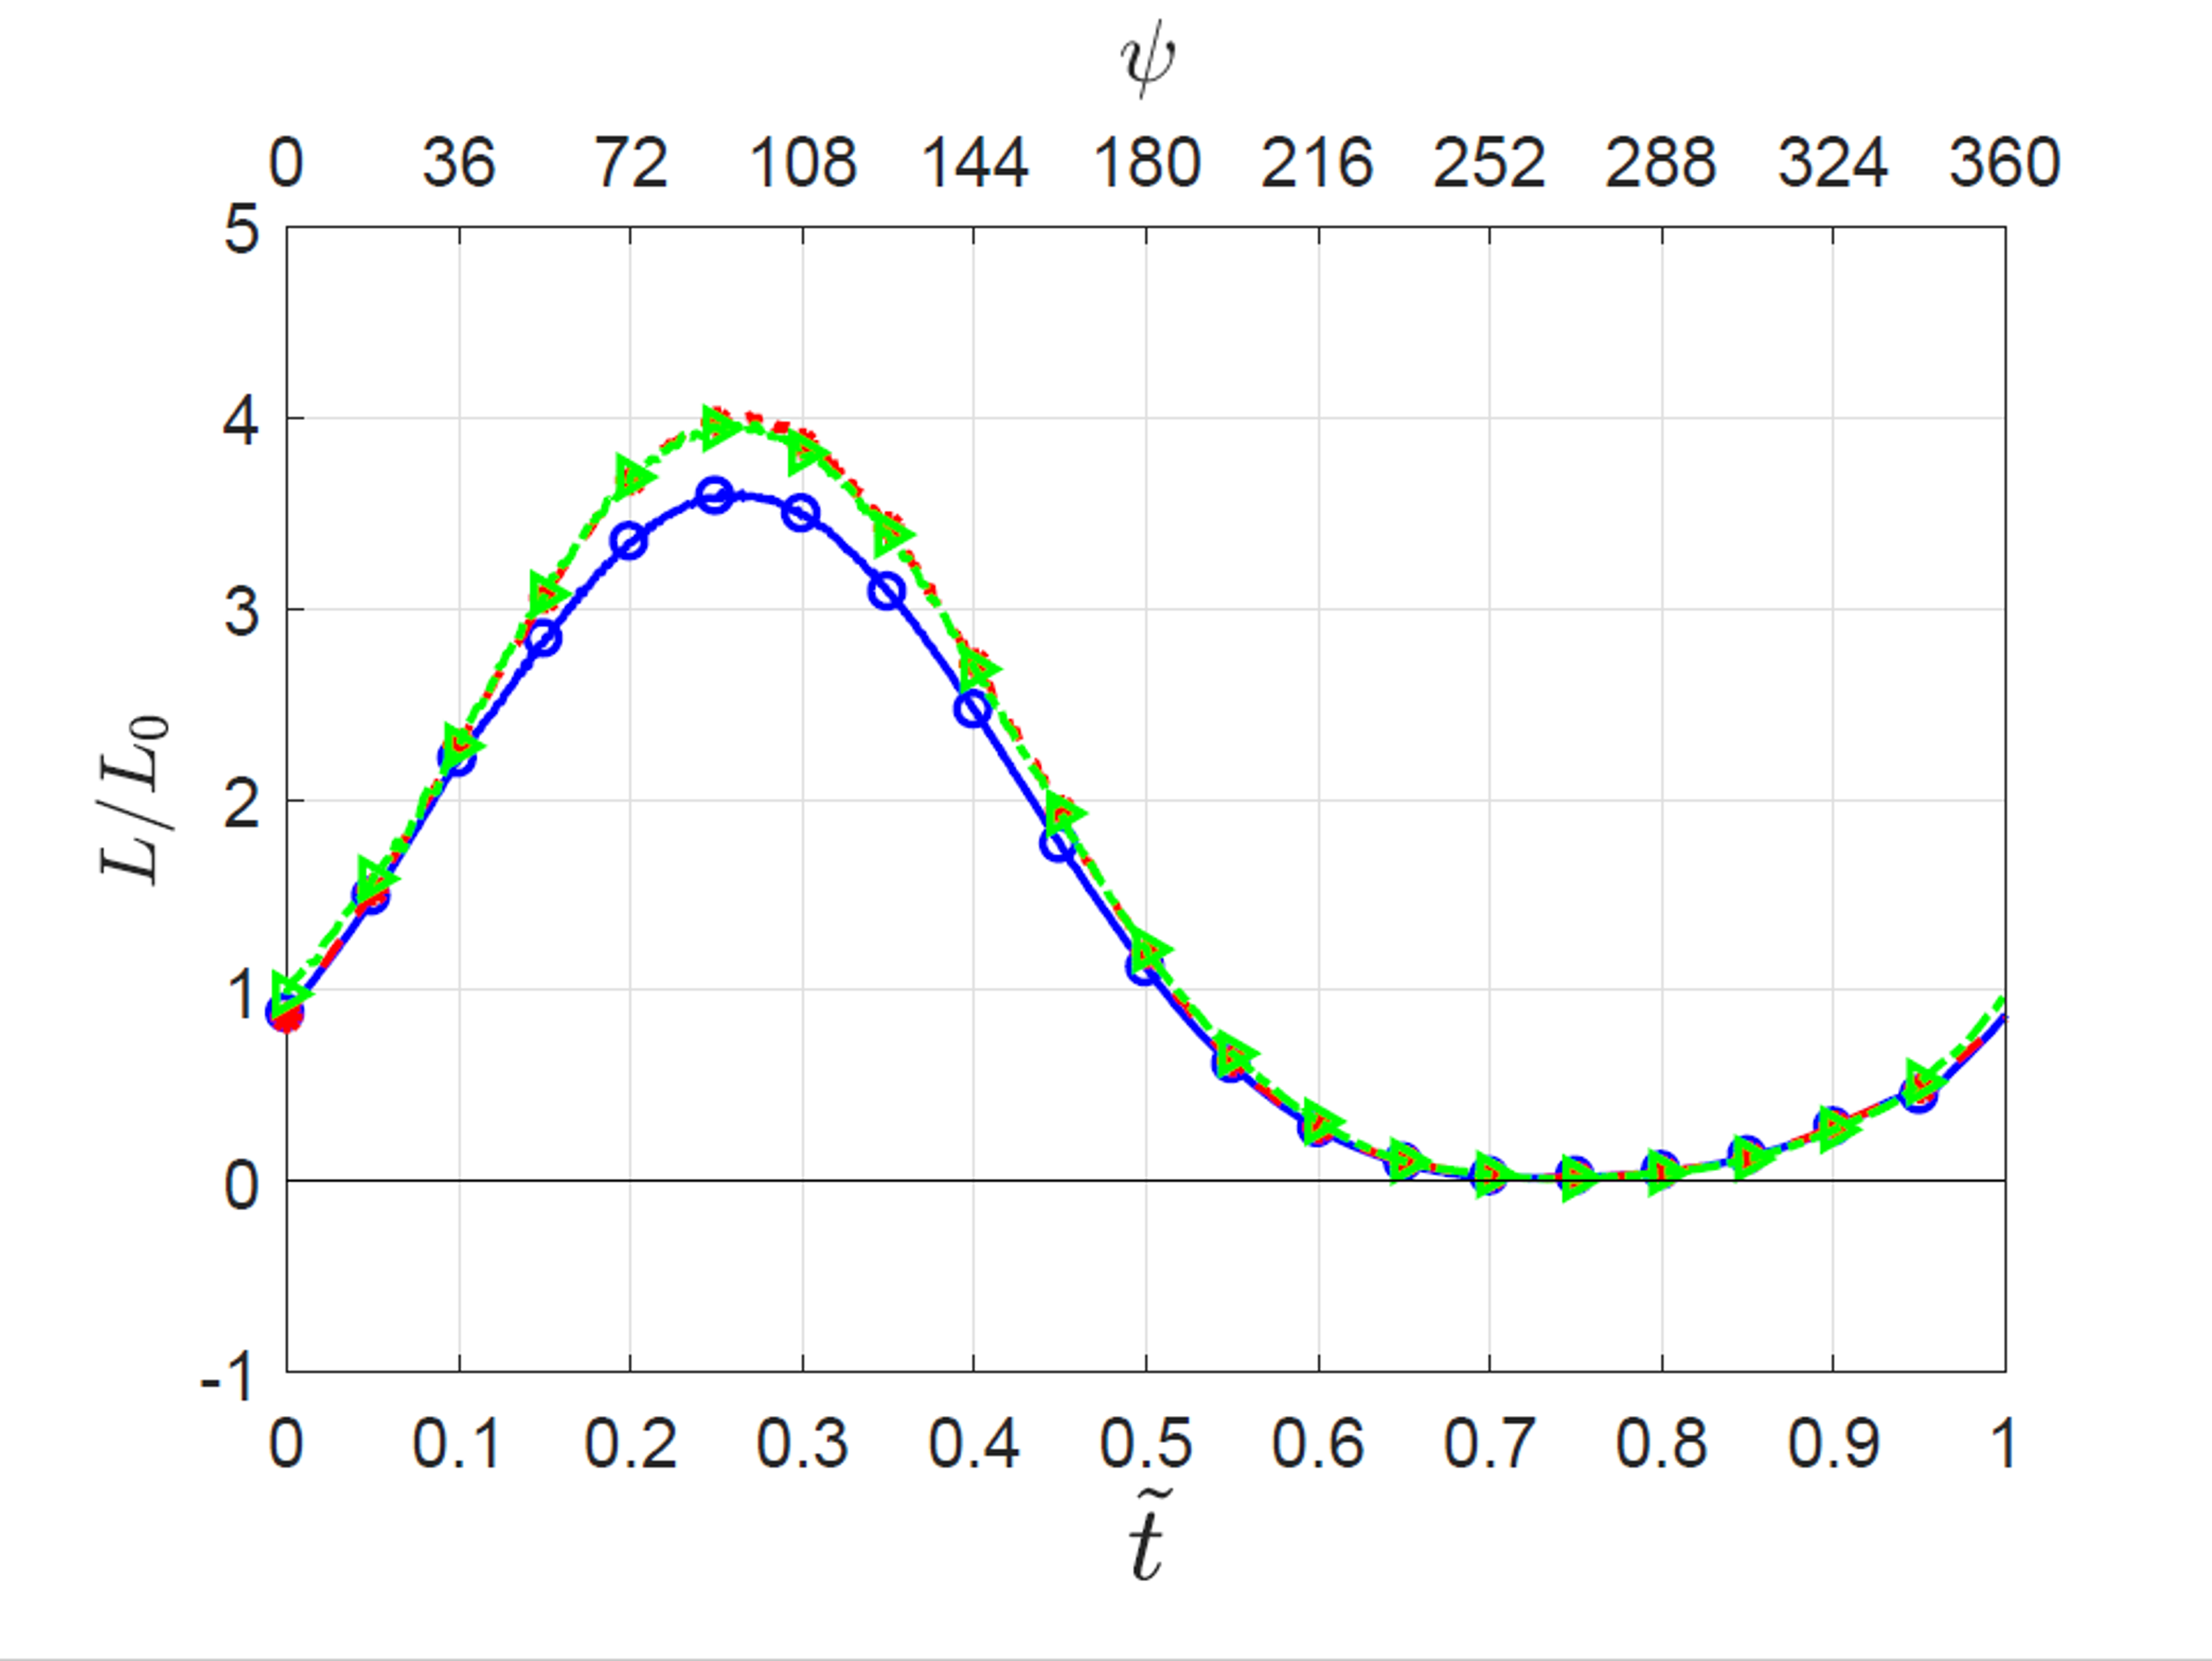
\includegraphics[width=1\textwidth]{figures/lift_Re_effect_lambda_1pt0.png}
		\subcaption{$\mu_{sect} = 1.0$}
		\label{fig:lift_Re_comparision_lambda_1p0}
	\end{subfigure}
 	\begin{subfigure}{0.5\textwidth}
		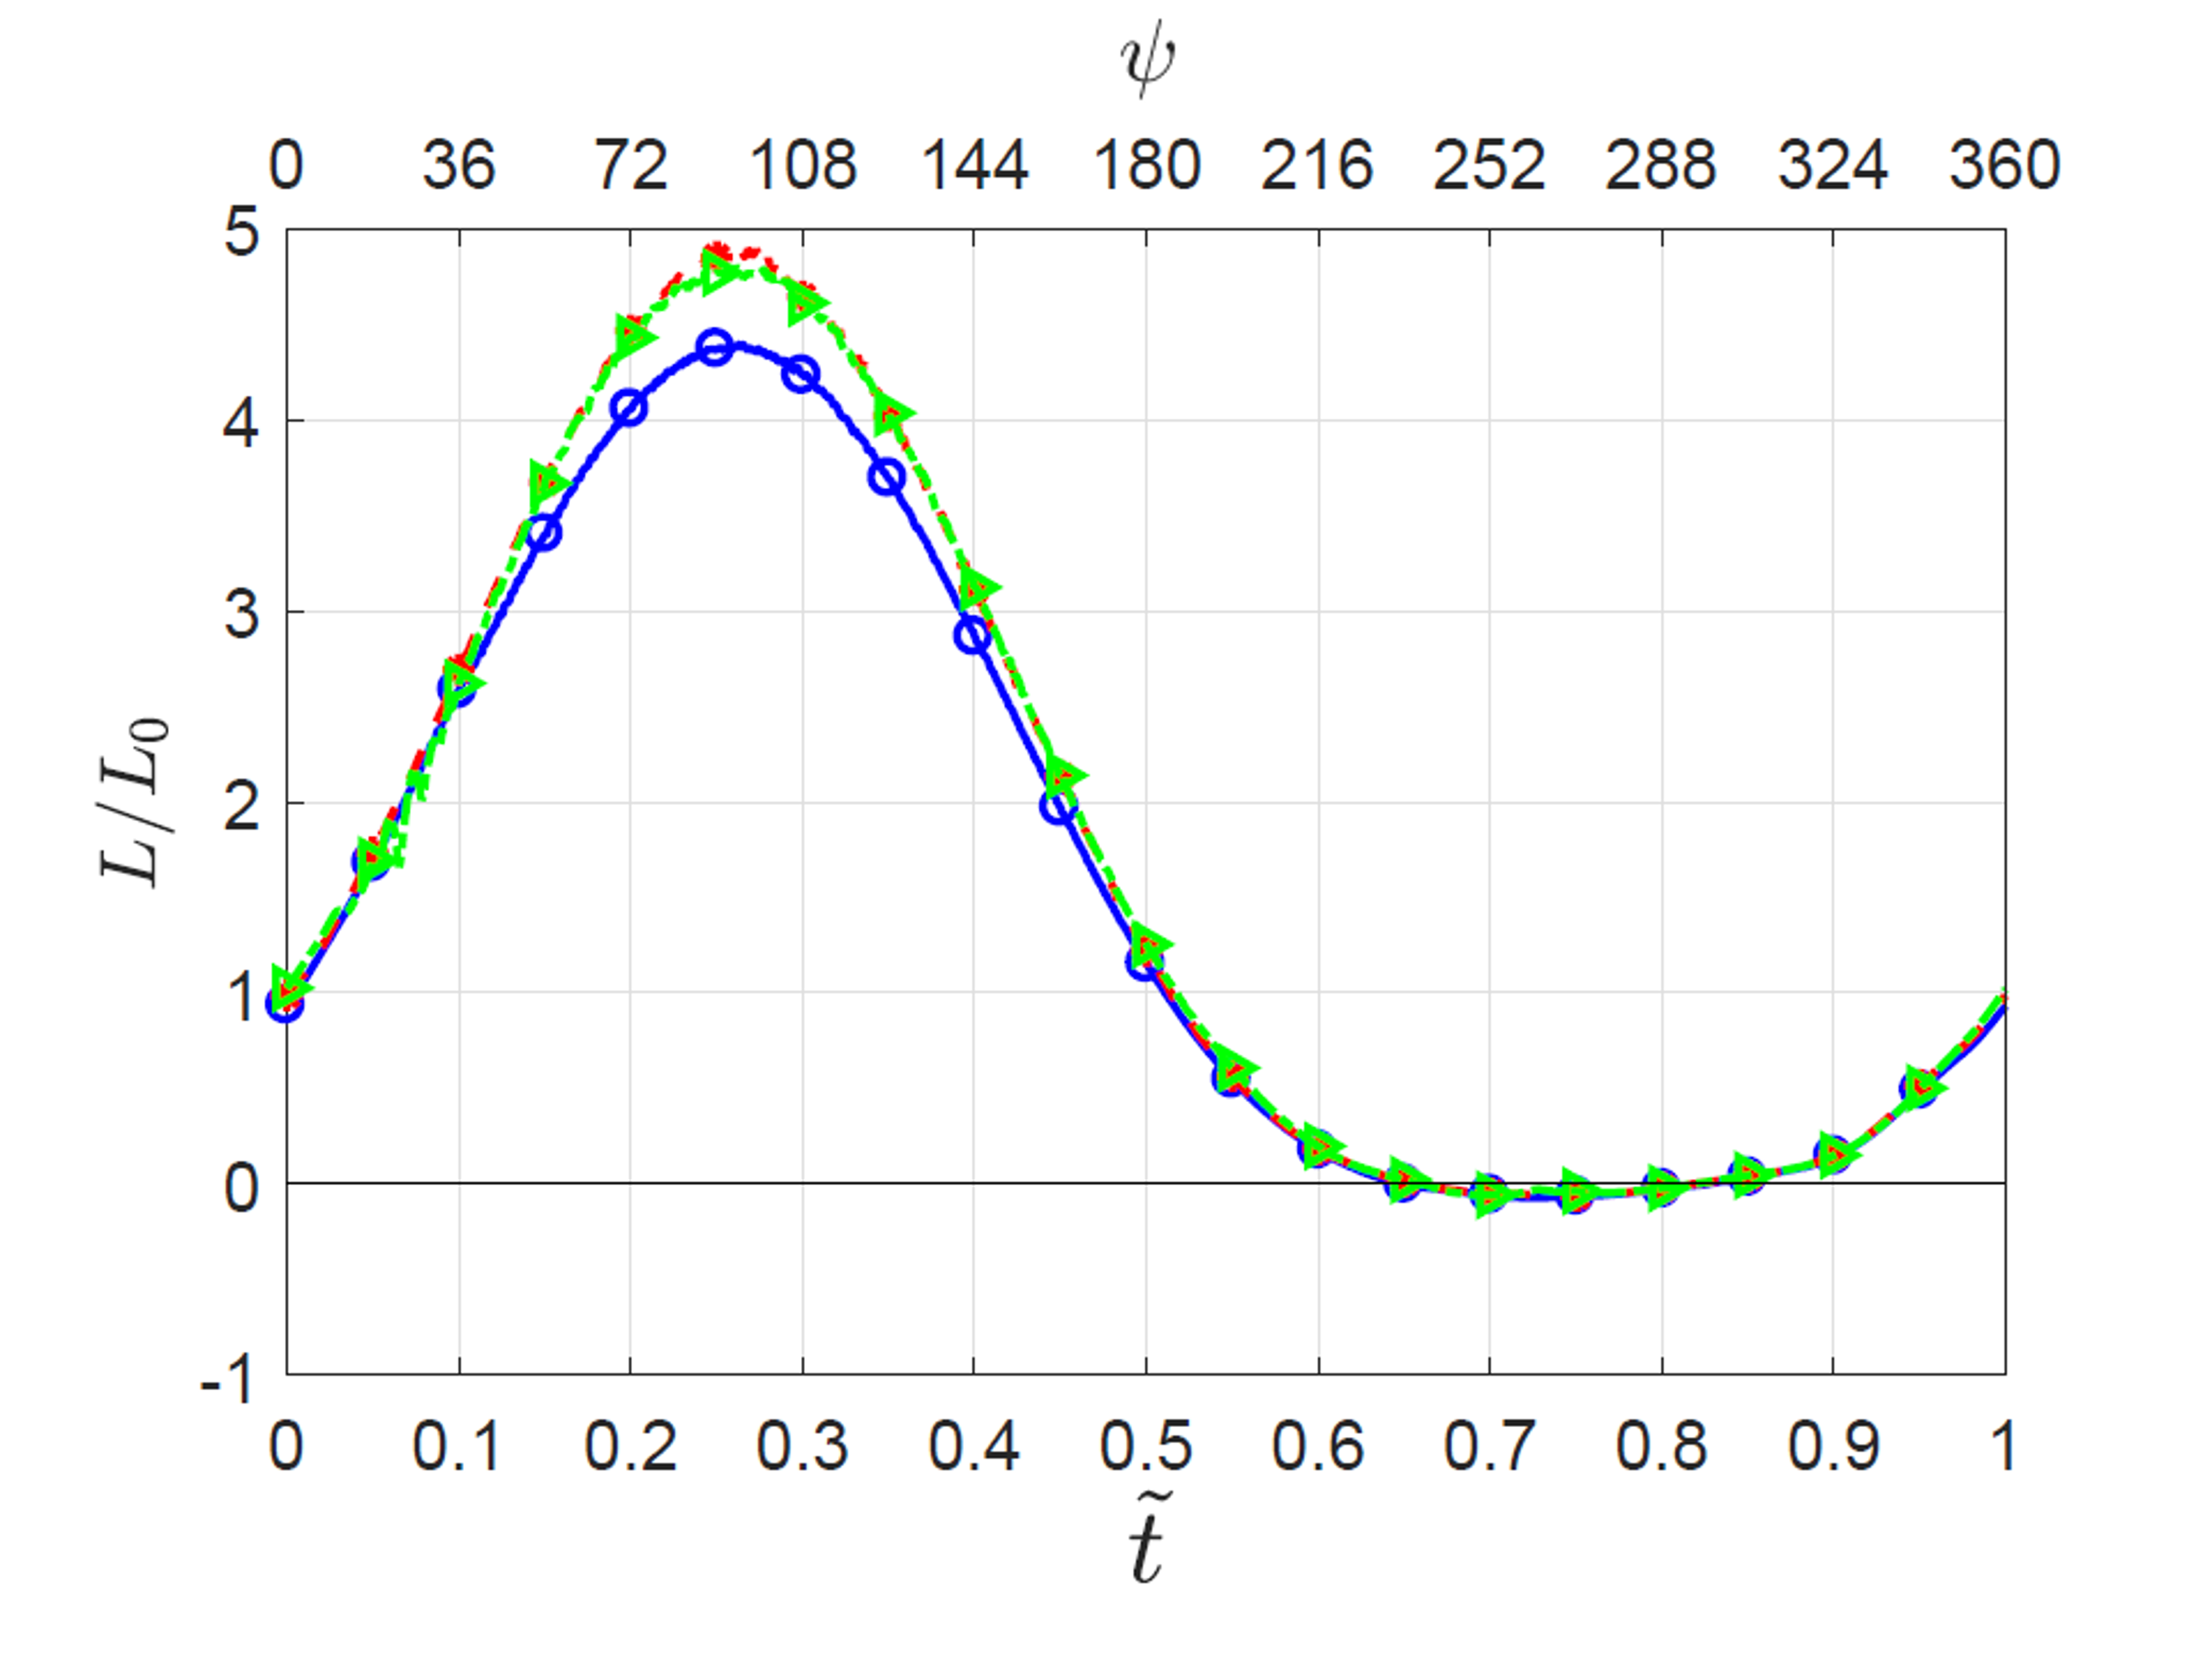
\includegraphics[width=1\textwidth]{figures/lift_Re_effect_lambda_1pt2.png}
        \subcaption{$\mu_{sect} = 1.2$}
		\label{fig:lift_Re_comparision_lambda_1p2}
	\end{subfigure}

 	\caption{Normalized lift force for $Re$=40,000 (green line with open triangles), 200,000 (red line with solid circles) and 1,000,000 (blue line with open circles) at $\mu_{sect}$=1.0 and 1.2}
 	\label{fig:lift_comparison}
\end{figure}

Lift force is shown in Figure \ref{fig:lift_comparison}.
Lift is normalized by its static counterpart, i.e., $L_0$ is the average or steady lift for the static airfoil at the mean Reynolds number over the surging cycle.
This normalization was used in our previous study with $Re$=40,000~\cite{bib:kocher_scitech2017} to compare against the experimental data of \cite{bib:granlund2016}, where a good agreement was shown between the experimental and simulation data.
Data is phase averaged over 4 cycles.
%%%We note that the averaged drag data exhibits fluctuations which is due to the presence of a turbulent flow, especially during the advancing phase of the cycle with a higher relative velocity or Reynolds number.
%%%However, these fluctuations are marginal in nature and averaging over additional cycles will be useful.

Overall, the lift force follows a similar qualitative trend for all the cases.
Maximum lift is achieved at $\tilde{t}=0.25$, which is expected as the airfoil achieves maximum relative velocity at that point.
After $\tilde{t}=0.25$, the lift starts decreasing as the airfoil begins to decelerate and enters the retreating phase. 
The lift keeps decreasing till about $\tilde{t}=0.65$ and plateaus or reaches a value close to zero during the middle of the retreating phase (i.e., around $\tilde{t}=0.75$ when the airfoil is at its minimum relative velocity).
We note that for both advance ratios of $\mu_{sect}$=1.0 and 1.2 a zero relative velocity is attained and for the higher advance ratio of $\mu_{sect}$=1.2 the relative velocity also becomes negative.
Lift starts to recover after $\tilde{t}=0.75$ as the airfoil starts accelerating again.
For each advance ratio, the normalized lift during the advancing phase for $Re$=1,000,000 is slightly smaller compared to the other two Reynolds numbers, see Figure \ref{fig:lift_Re_comparision_lambda_1p0} or Figure \ref{fig:lift_Re_comparision_lambda_1p2}.
The normalized lift is very similar between $Re$=40,000 and 200,000 cases.
The peak normalized lift is about 9\% lower for the highest Reynolds number case as compared to the lower Reynolds number cases for each advance ratio.
On the other hand, for a given Reynolds number the normalized lift is higher for the higher advance ratio, which is expected due to the higher dynamic pressure in any given instance or phase in the surging cycle.
The peak normalized lift is about 21\% higher for the higher advance ratio case as compared to the lower advance ratio case for each Reynolds number, which is the difference in the peak dynamic pressure between the two advance ratios.

\subsection{Flowfield: Spanwise Vorticity}

In this section, we present spanwise vorticity over the cycle at 8 different phases of $\psi$ = $195^\circ$, $225^\circ$, $240^\circ$, $255^\circ$, $270^\circ$, $315^\circ$, $330^\circ$,and $345^\circ$, which are all in the retreating part of the surging cycle.
We focus our attention on the leading edge vortex (LEV) which is the dominant flow feature.
It forms and advects during the retreating part, while in the advancing part the flow remains attached.
As noted earlier, data is phase averaged over 4 cycles.
In addition, averaging is also applied in the spanwise direction.

Figure \ref{fig:vortScreen_1pt0} shows the spanwise vorticity for the lower advance ratio of $\mu_{sect}$=1.0.
The voriticy range is selected to be [-10,10]$\times U_\infty /C$.
At $\psi$=$195^\circ$, the flow over the airfoil is mostly attached, however, the boundary layer is relatively thick as the airfoil is decelerating, see Figures~\ref{fig:Re_40k_1pt0_phi195}, \ref{fig:Re_200k_1pt0_phi195} and \ref{fig:Re_1m_1pt0_phi195}.
As expected, the boundary layer is much thicker for the lowest Reynolds number of $Re$=40,000 as compared to the other two higher Reynolds numbers.

\begin{figure}[H]
	\centering
	
	\begin{subfigure}[b]{0.32\textwidth}
		\centering
		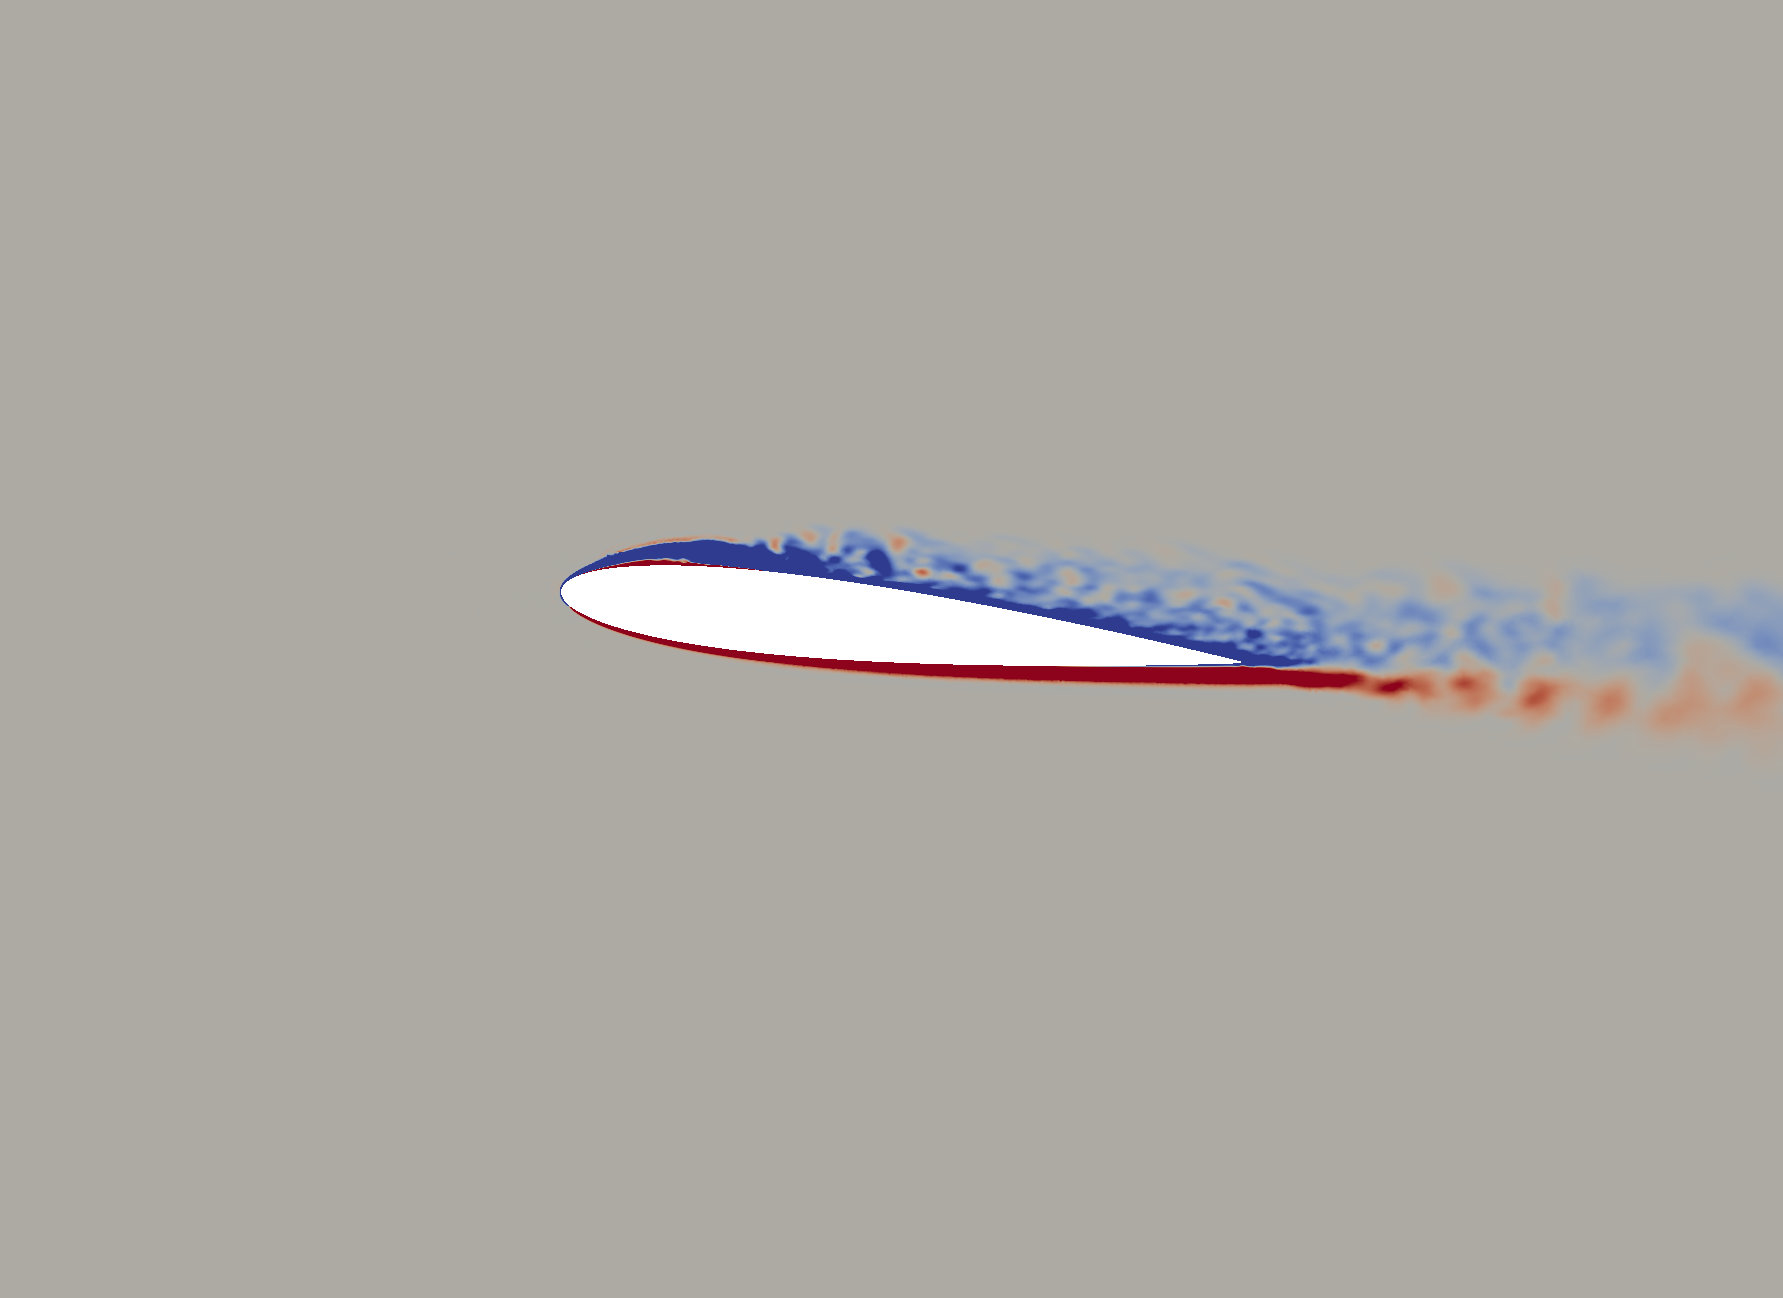
\includegraphics[width=1\textwidth]{figures/Vorticity_plots/Re_40k_1pt0/phase_195.png}
		\caption{$Re=4e4$, $\psi$ = $195^\circ$, $\tilde{t}=0.542$}
		\label{fig:Re_40k_1pt0_phi195}
	\end{subfigure}
	\begin{subfigure}[b]{0.32\textwidth}
		\centering
		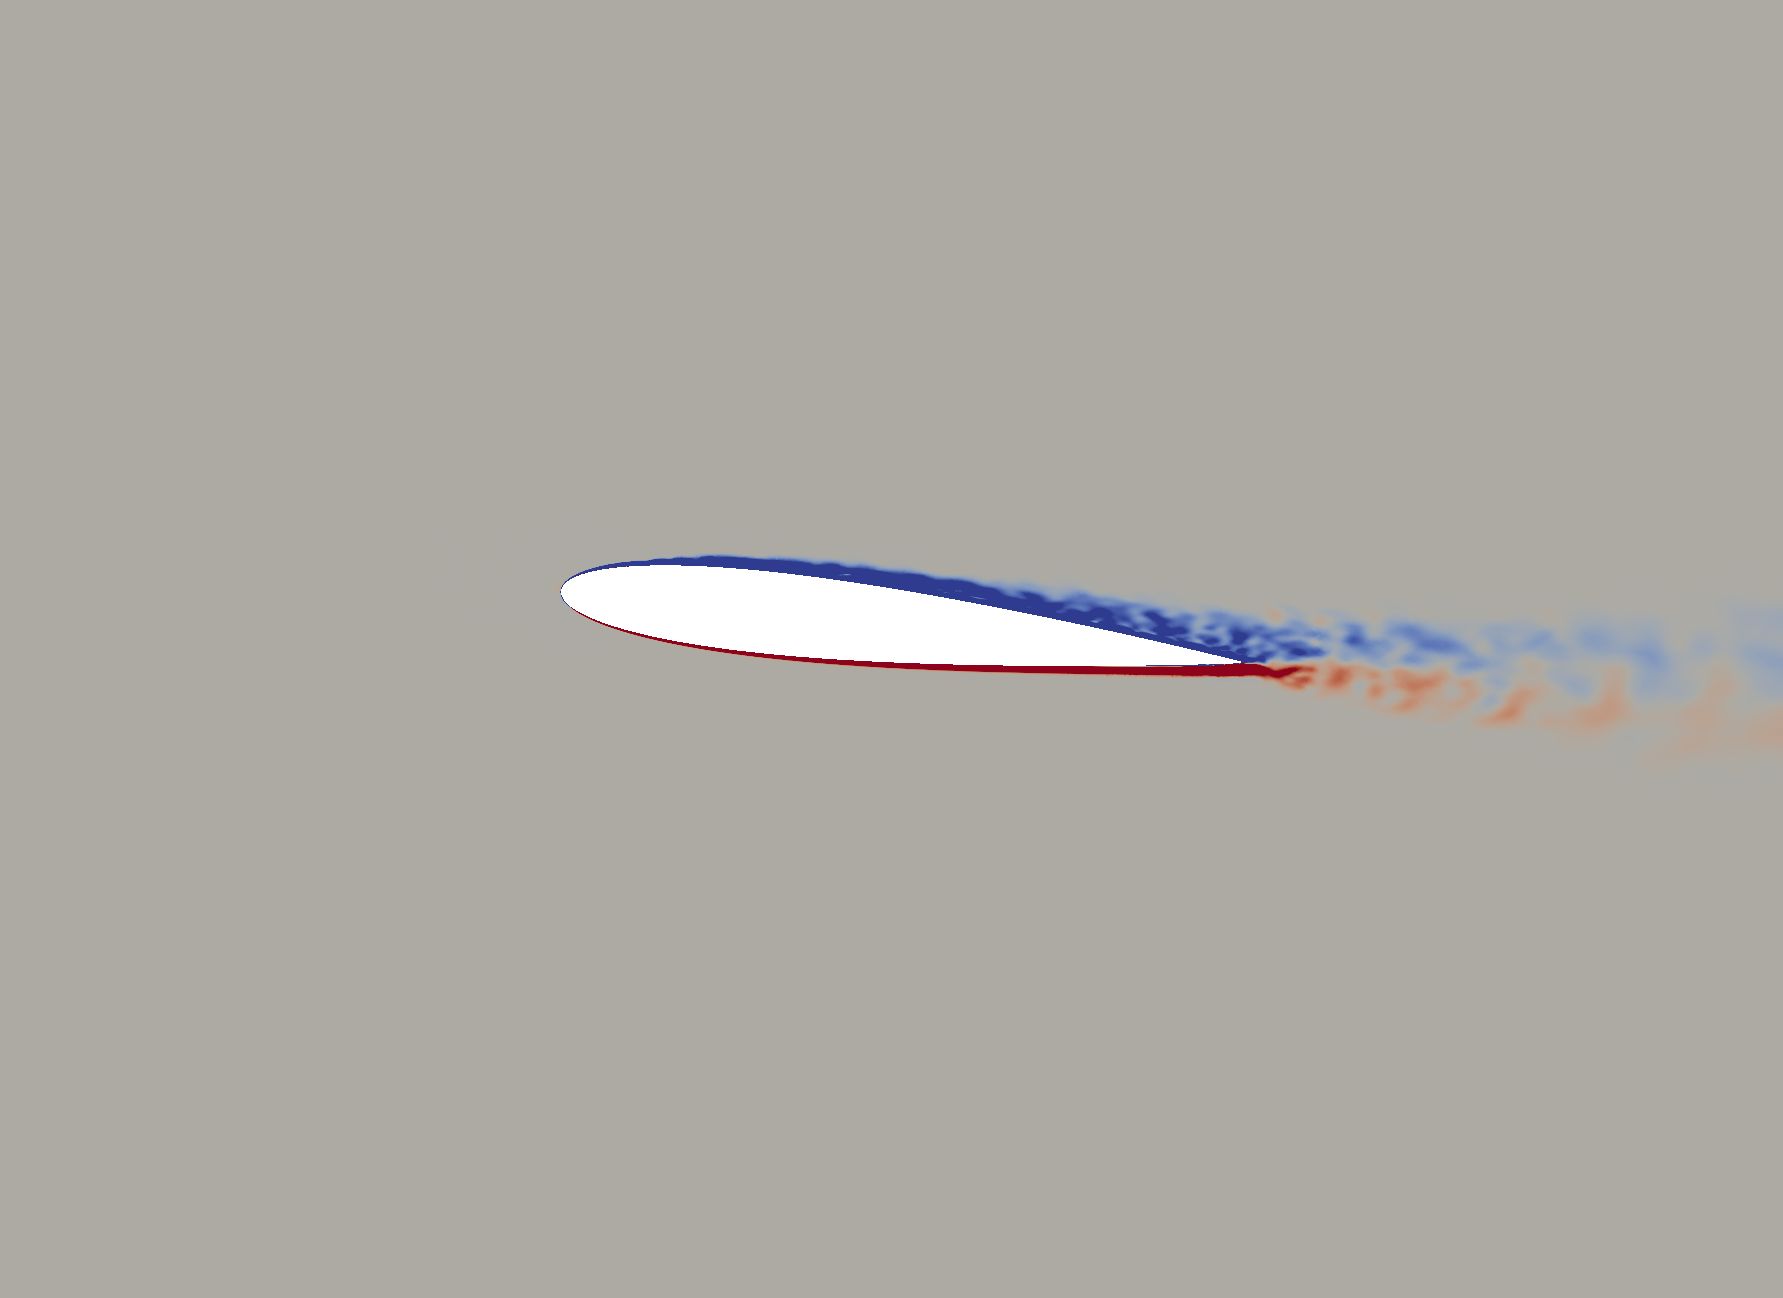
\includegraphics[width=1\textwidth]{figures/Vorticity_plots/Re_200k_1pt0/phase_195.png}
		\caption{$Re=2e5$, $\psi$ = $195^\circ$, $\tilde{t}=0.542$}
		\label{fig:Re_200k_1pt0_phi195}
	\end{subfigure}
	\begin{subfigure}[b]{0.32\textwidth}
		\centering
		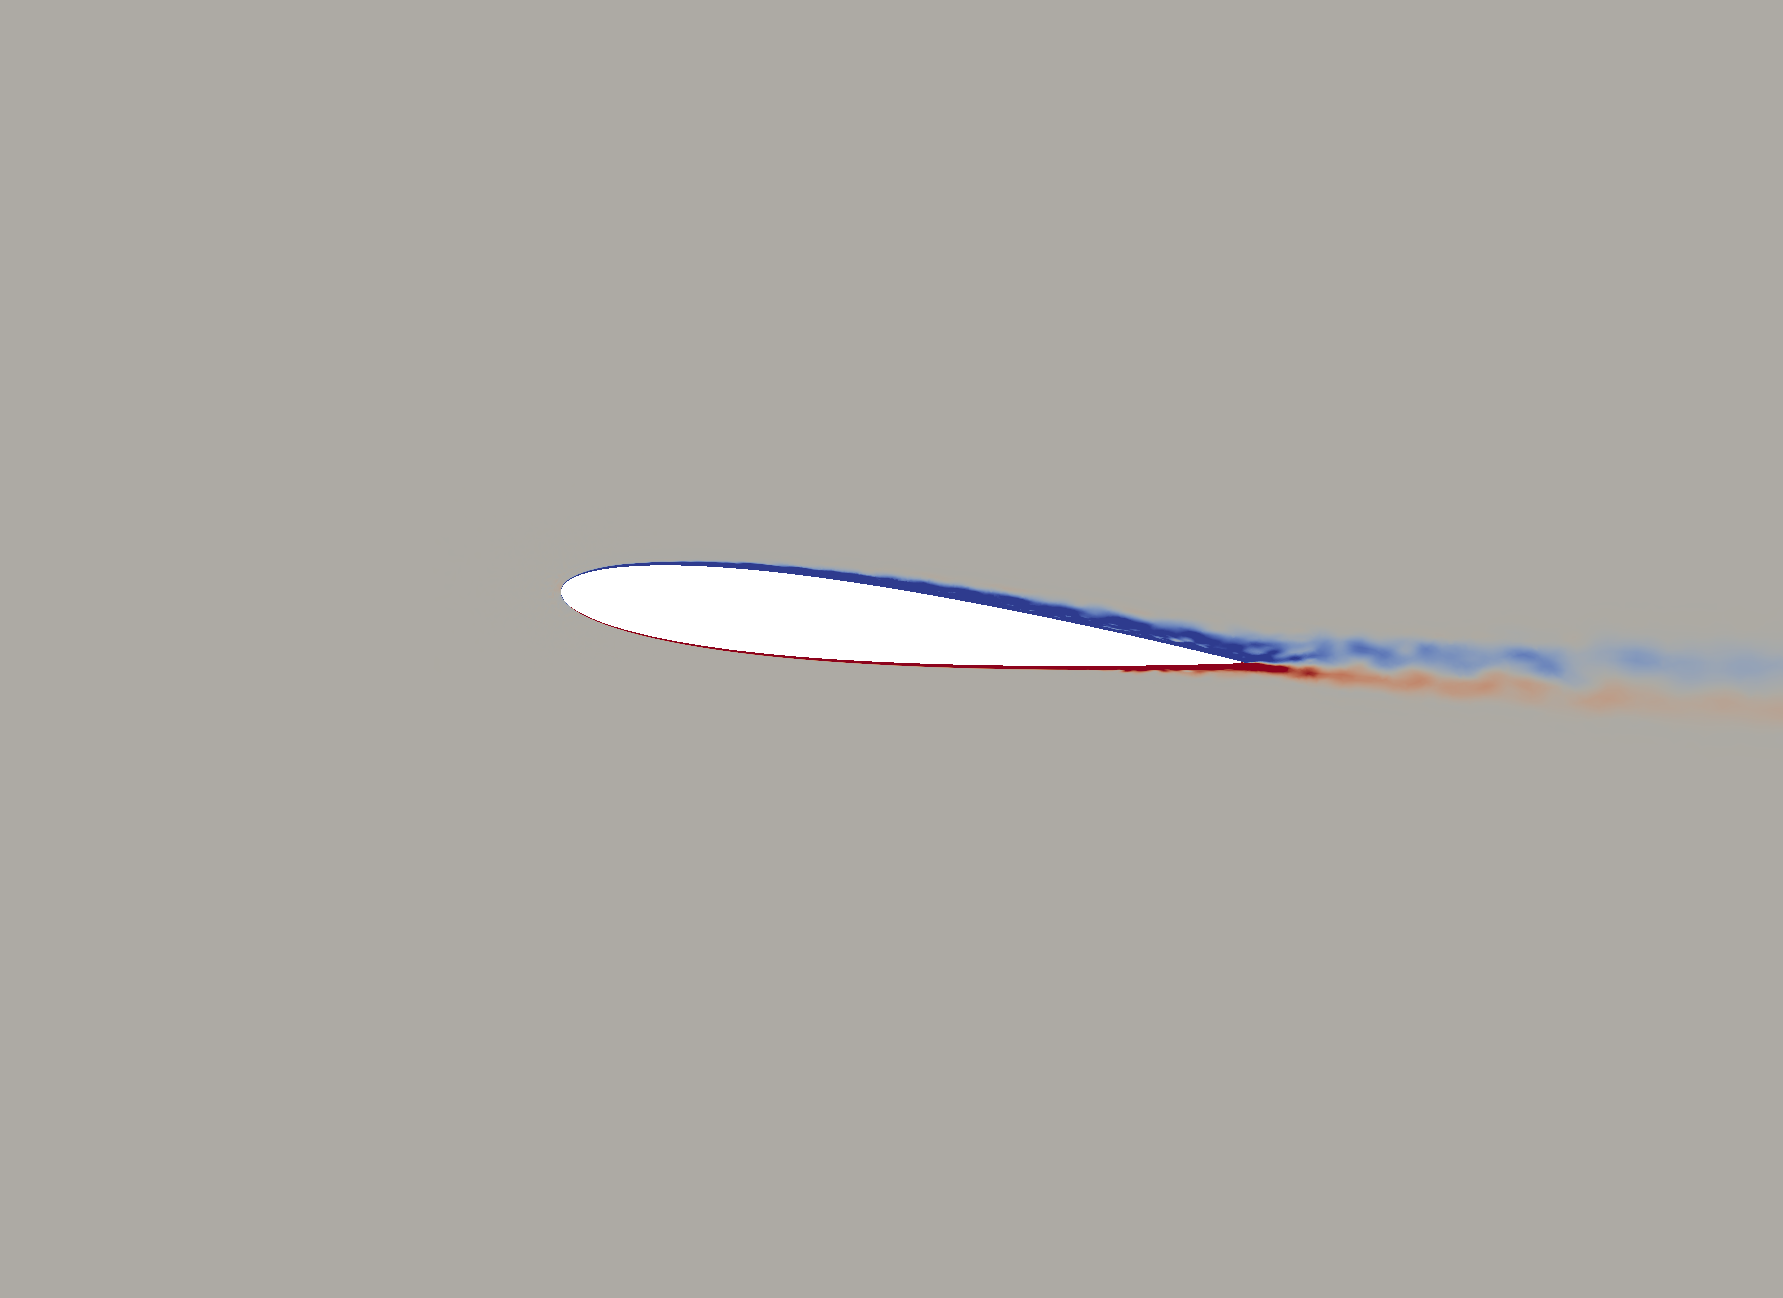
\includegraphics[width=1\textwidth]{figures/Vorticity_plots/Re_1m_1pt0/phase_195.png}
		\caption{$Re= 1e6$, $\psi$ = $195^\circ$, $\tilde{t}=0.542$}
		\label{fig:Re_1m_1pt0_phi195}
	\end{subfigure}
	
	\begin{subfigure}[b]{0.32\textwidth}
		\centering
		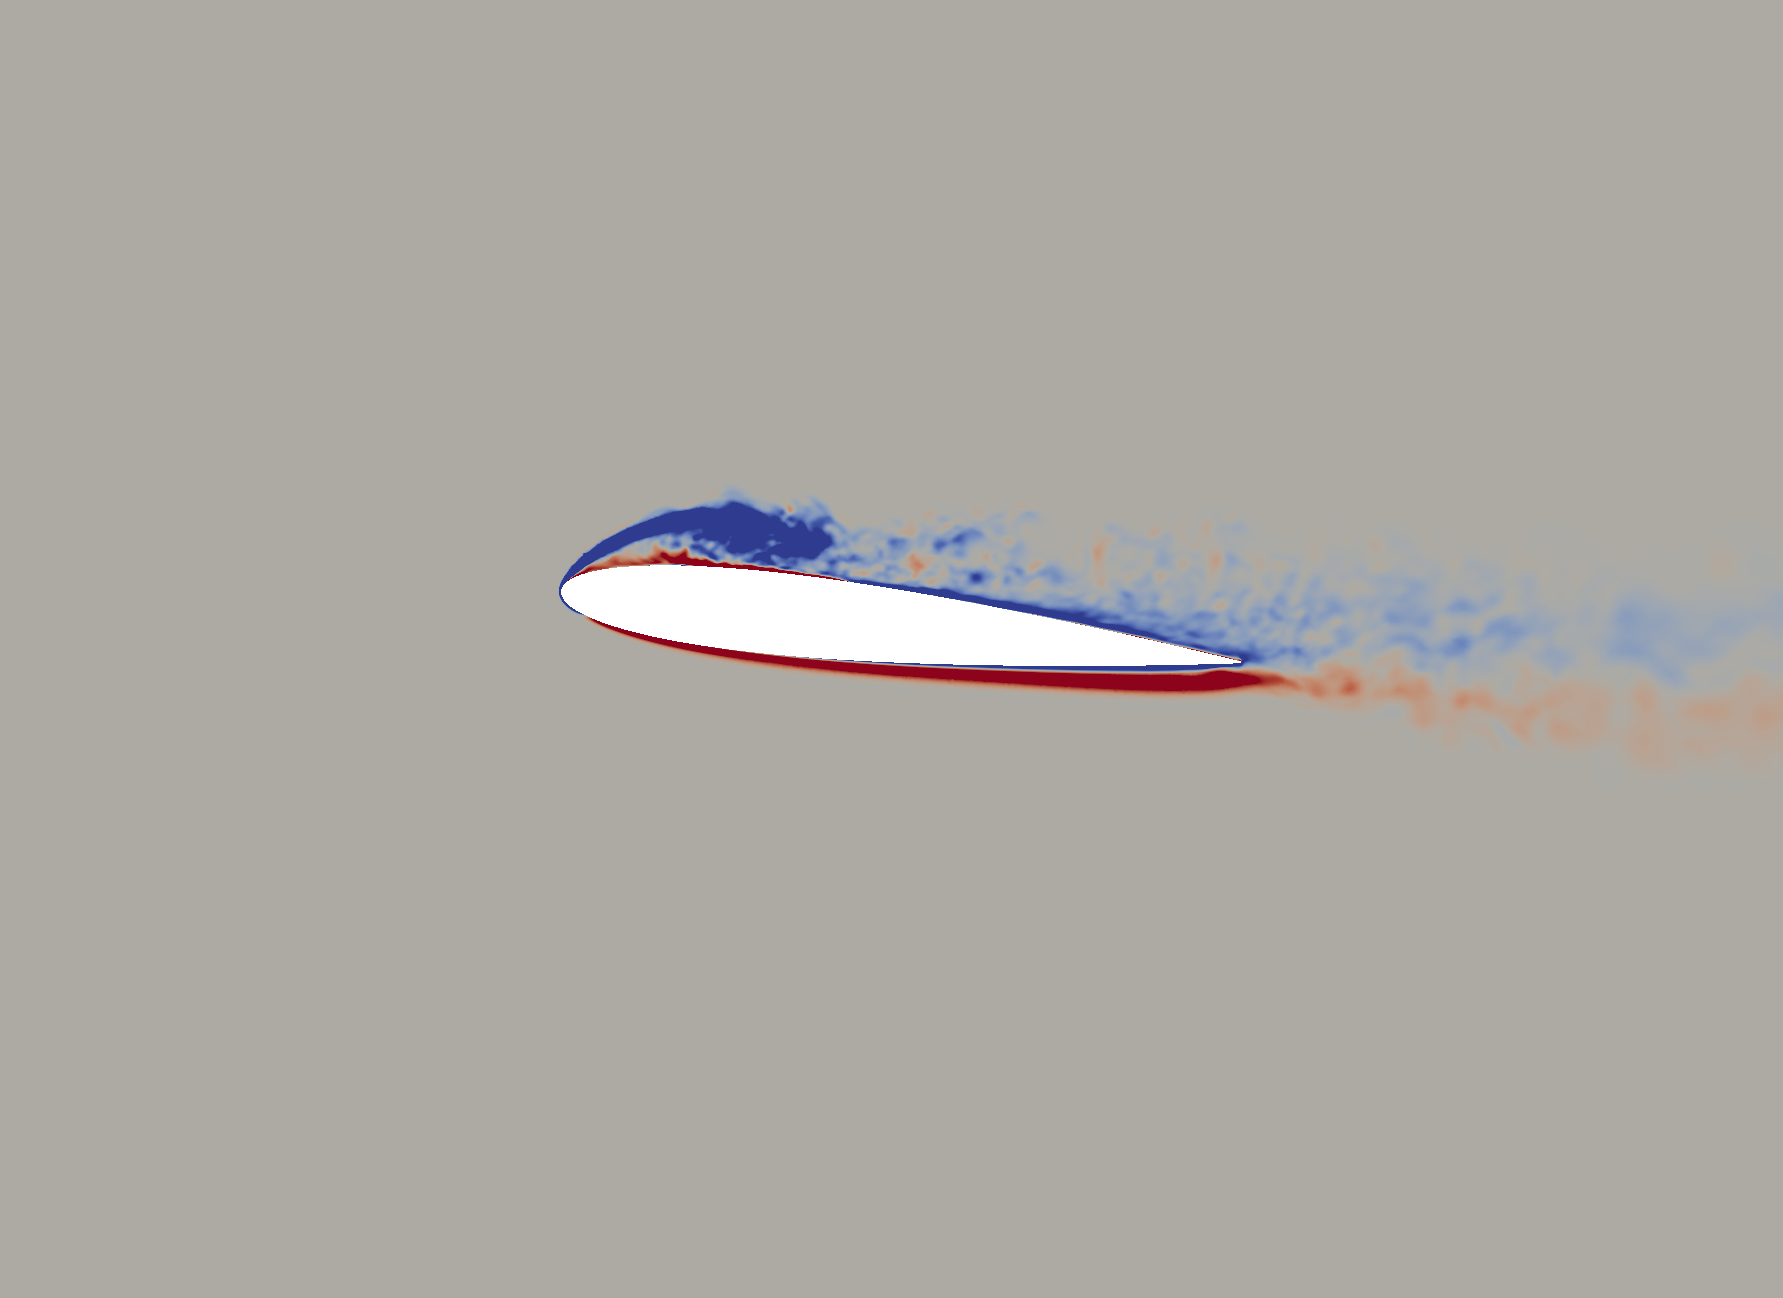
\includegraphics[width=1\textwidth]{figures/Vorticity_plots/Re_40k_1pt0/phase_225.png}
		\caption{$Re=4e4$, $\psi$ = $225^\circ$, $\tilde{t}=0.625$}
		\label{fig:Re_40k_1pt0_phi225}
	\end{subfigure}
	\begin{subfigure}[b]{0.32\textwidth}
		\centering
		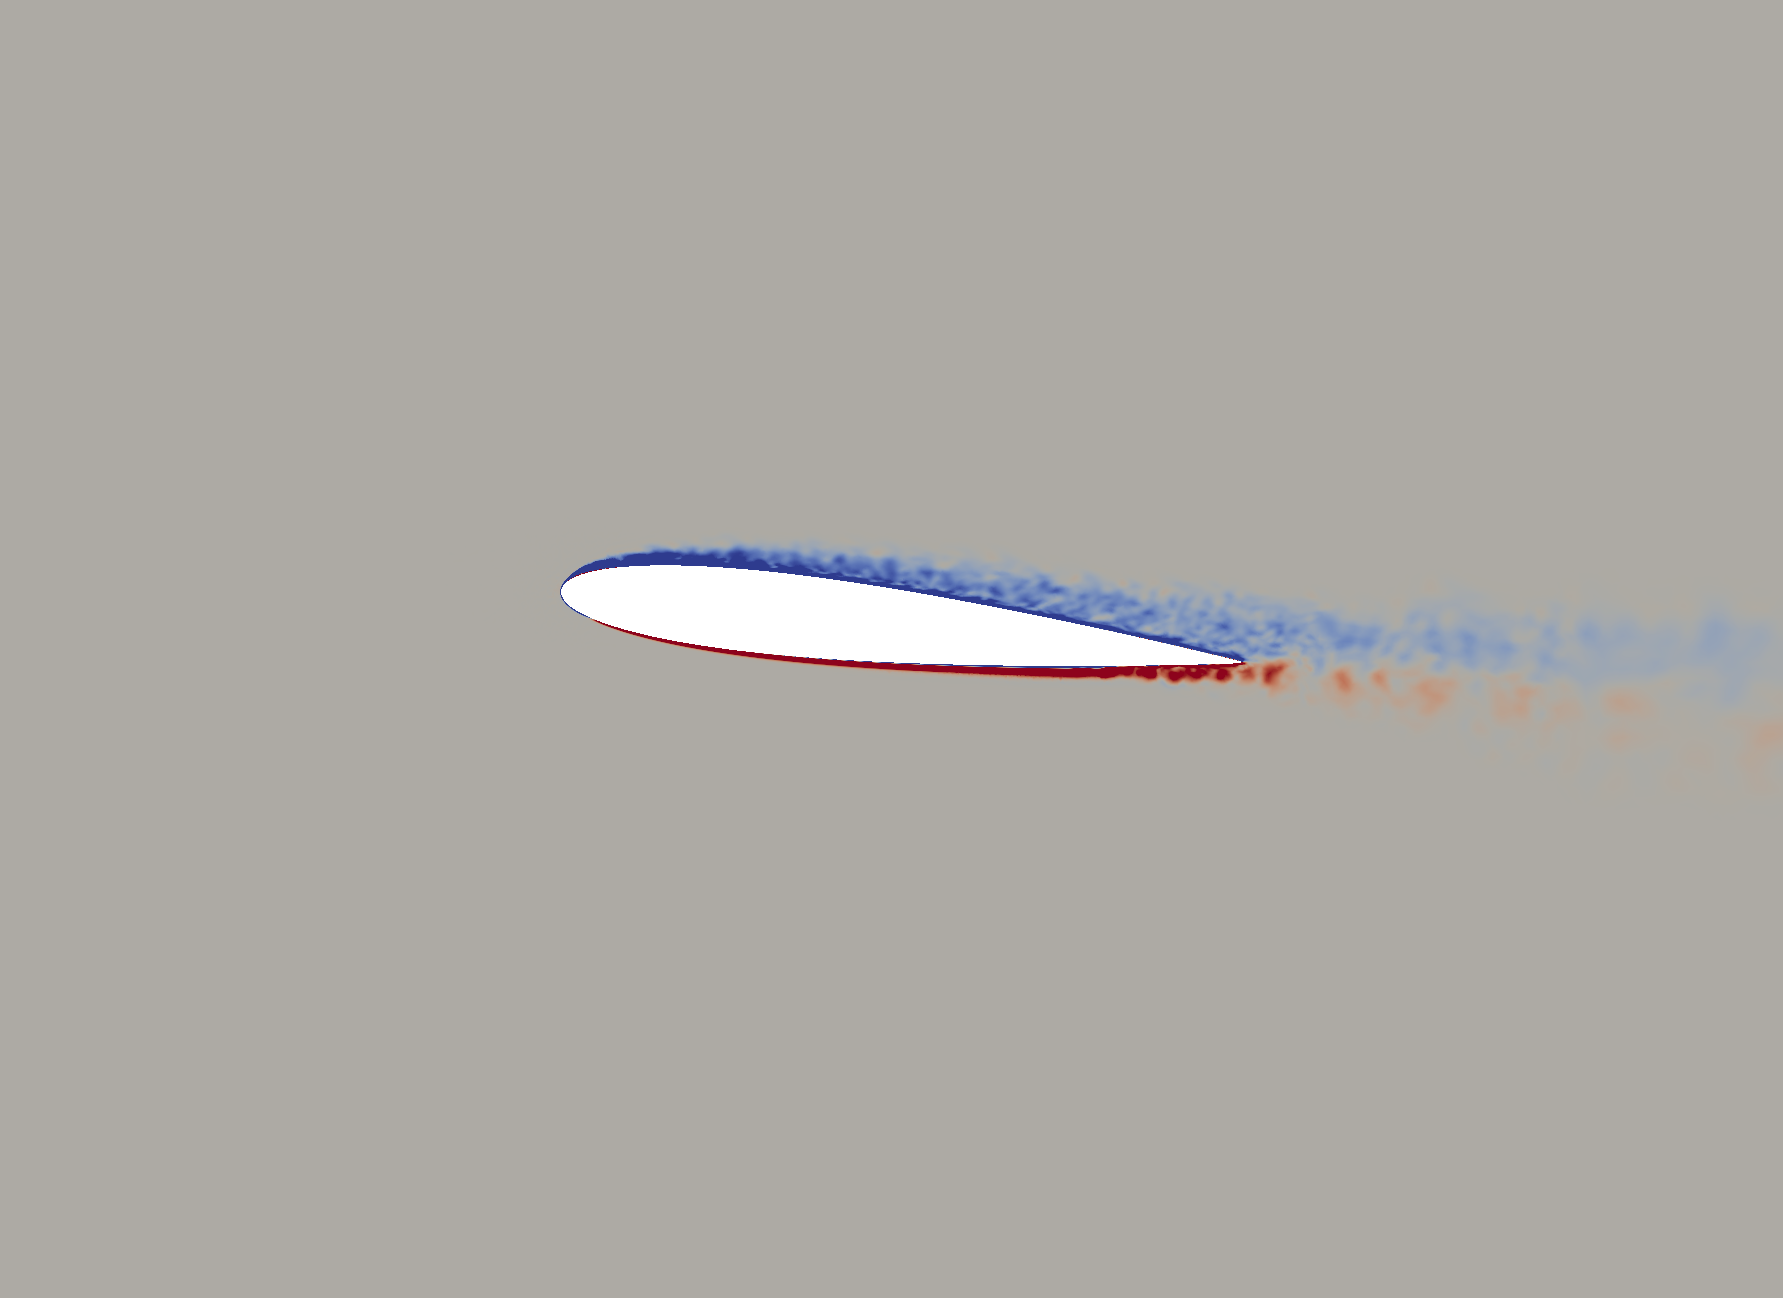
\includegraphics[width=1\textwidth]{figures/Vorticity_plots/Re_200k_1pt0/phase_225.png}
		\caption{$Re=2e5$, $\psi$ = $225^\circ$,  $\tilde{t}=0.625$}
		\label{fig:Re_200k_1pt0_phi225}
	\end{subfigure}
	\begin{subfigure}[b]{0.32\textwidth}
		\centering
		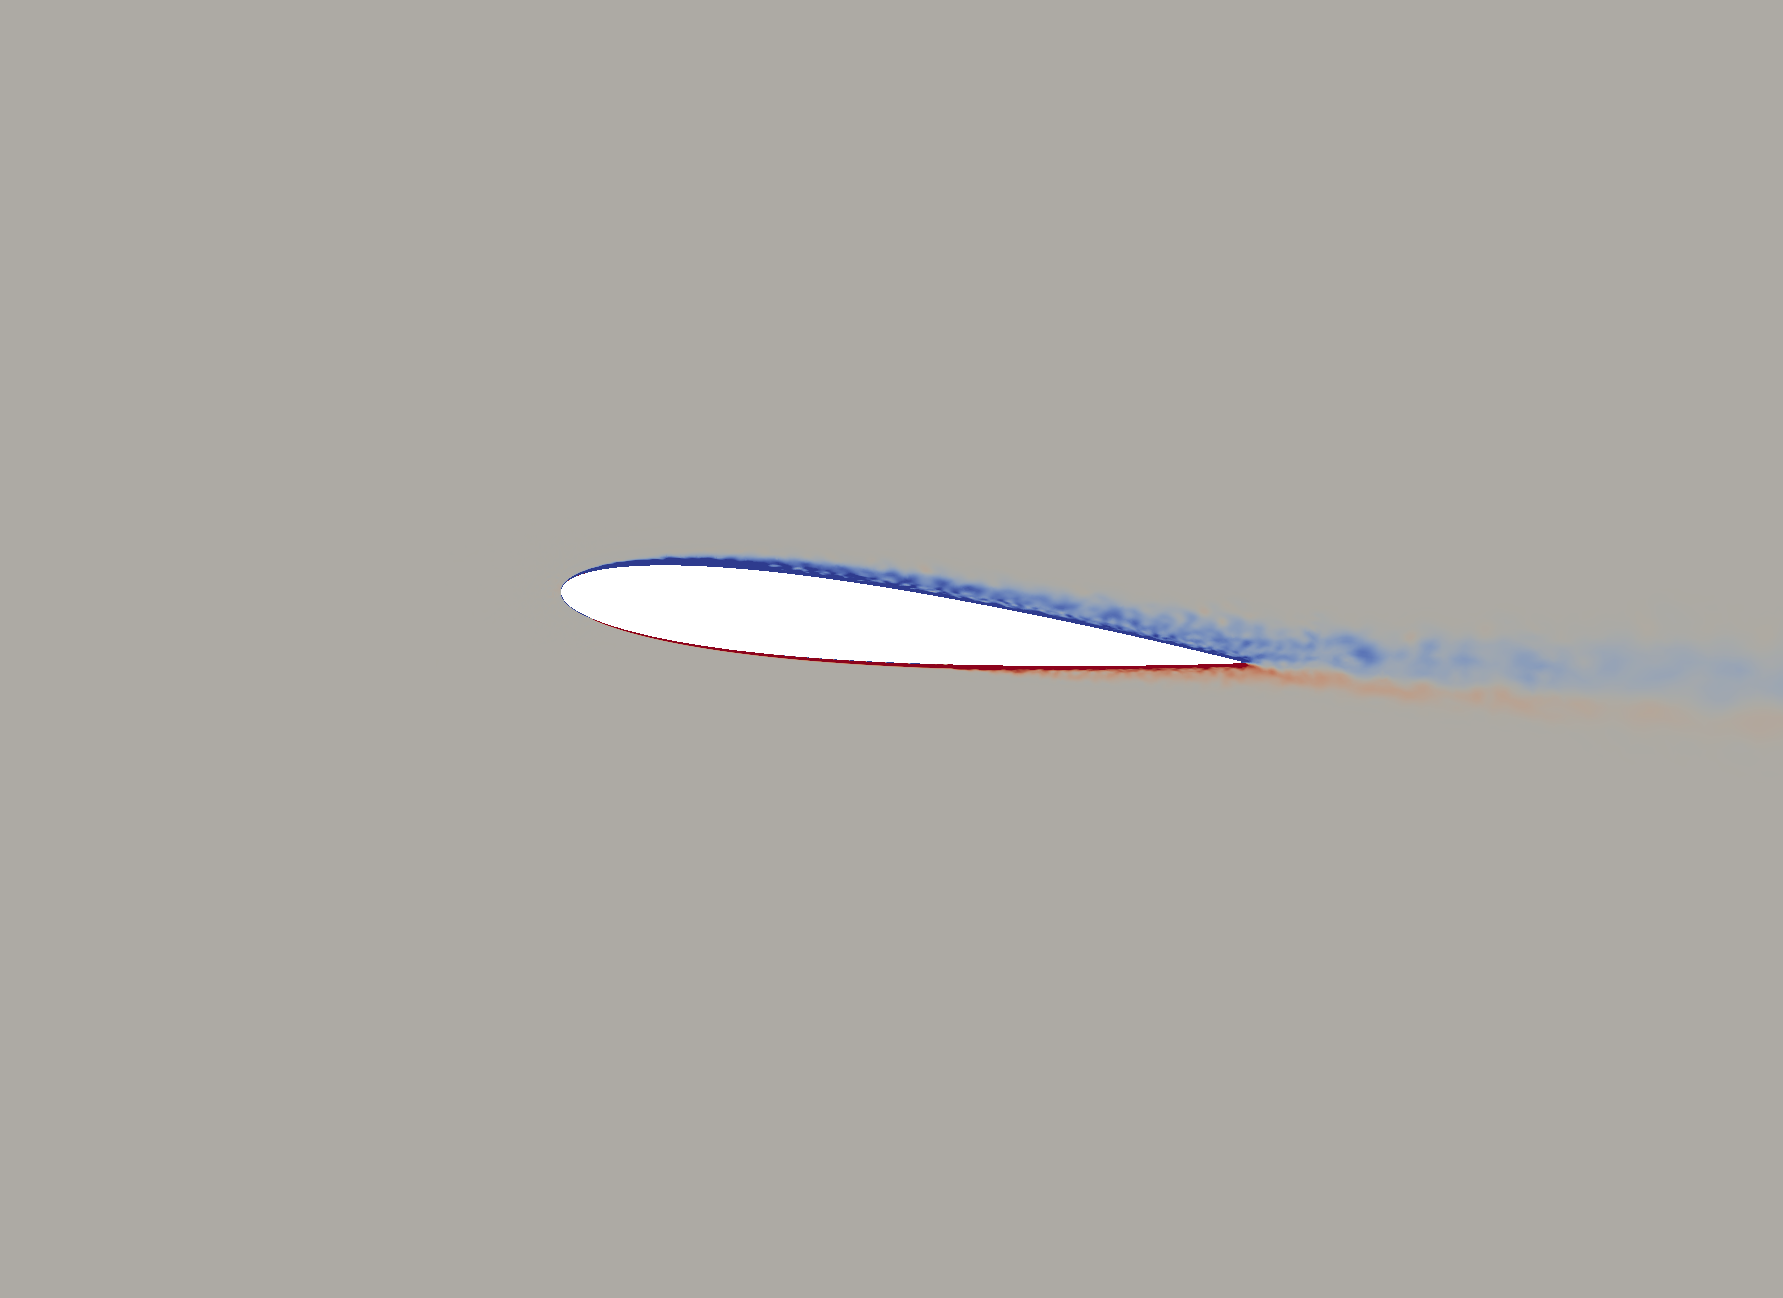
\includegraphics[width=1\textwidth]{figures/Vorticity_plots/Re_1m_1pt0/phase_225.png}
		\caption{$Re=1e6$, $\psi$ = $225^\circ$,  $\tilde{t}=0.625$}
		\label{fig:Re_1m_1pt0_phi225}
	\end{subfigure}
	
	\begin{subfigure}[b]{0.32\textwidth}
		\centering
		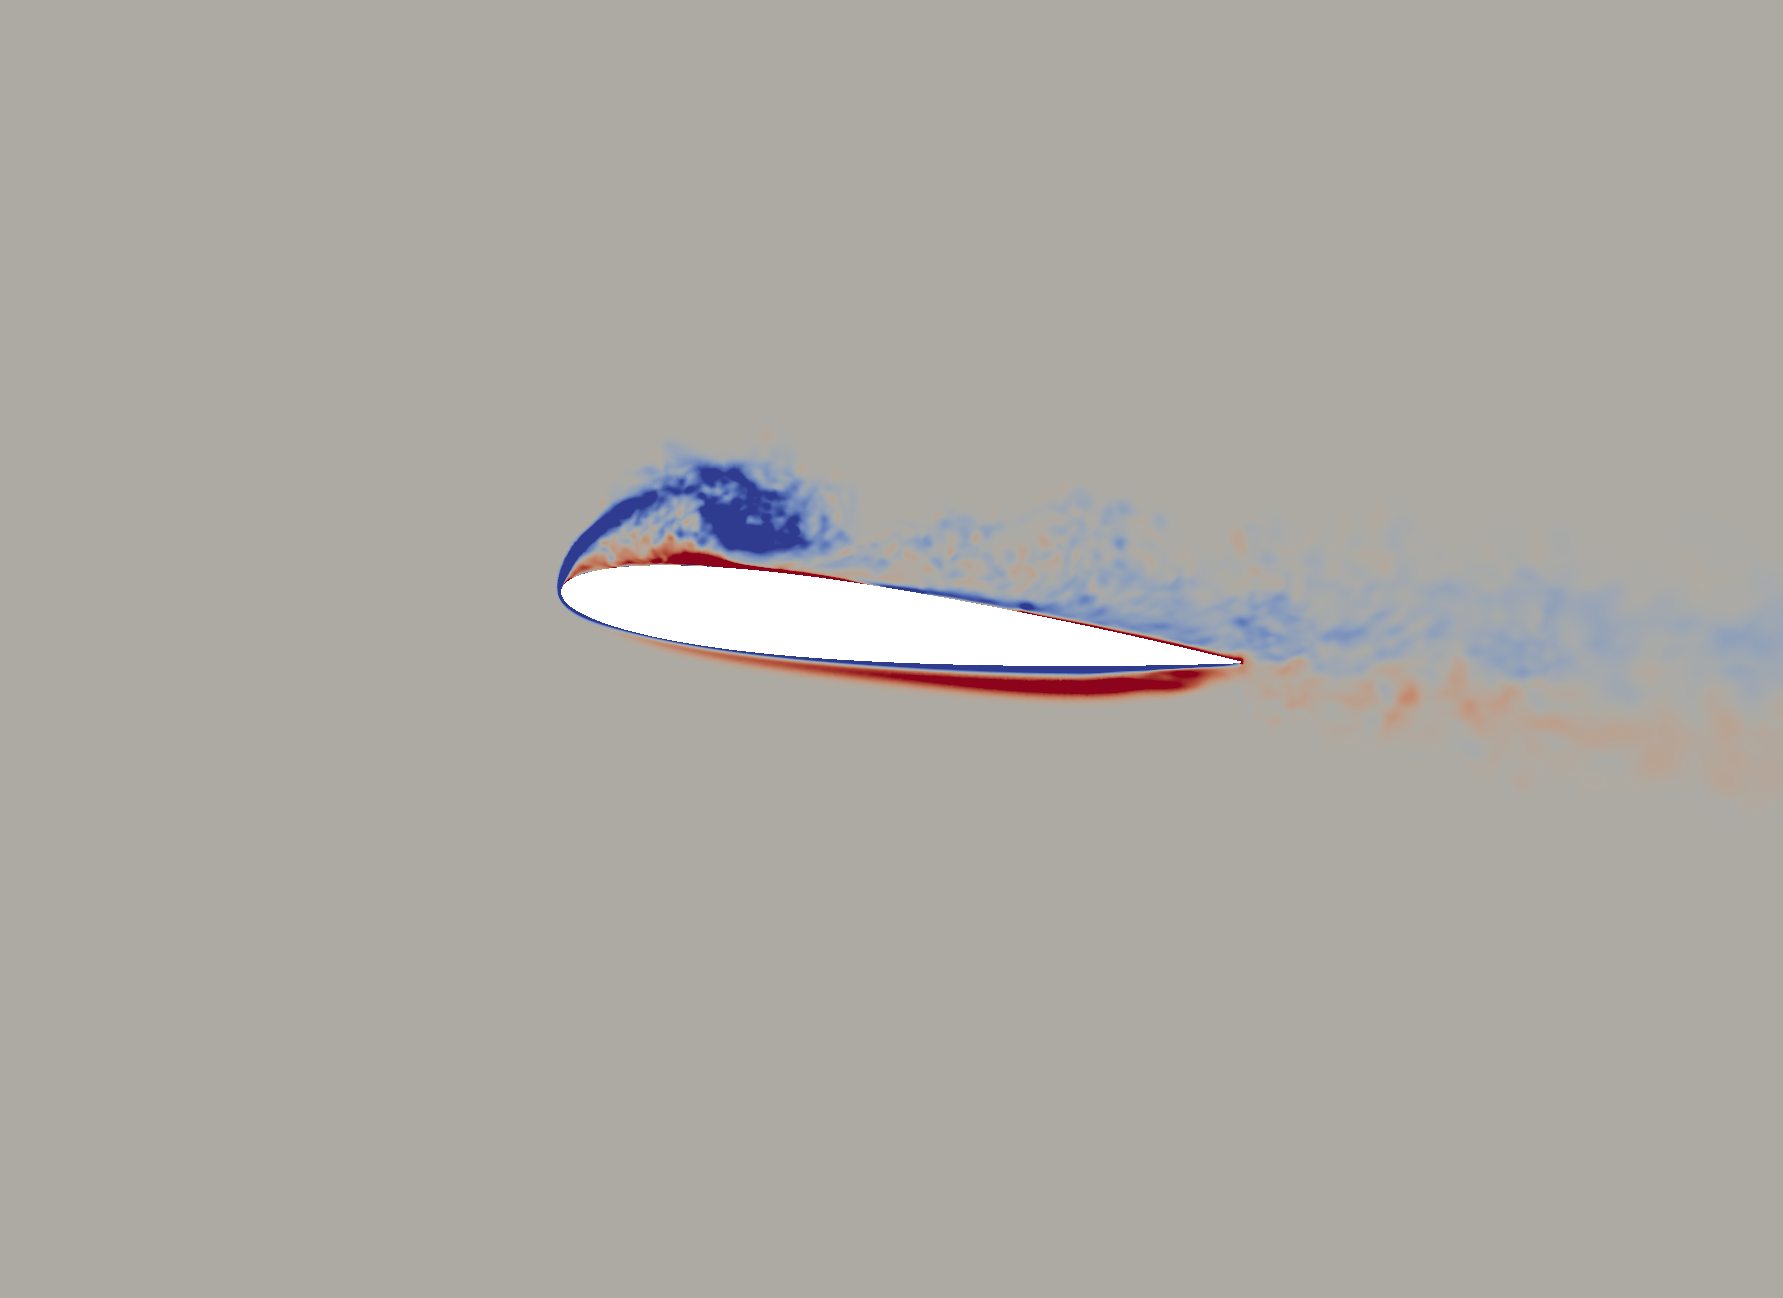
\includegraphics[width=1\textwidth]{figures/Vorticity_plots/Re_40k_1pt0/phase_240.png}
		\caption{$Re=4e4$, $\psi$ = $240^\circ$, $\tilde{t}=0.667$}
		\label{fig:Re_40k_1pt0_phi240}
	\end{subfigure}
	\begin{subfigure}[b]{0.32\textwidth}
		\centering
		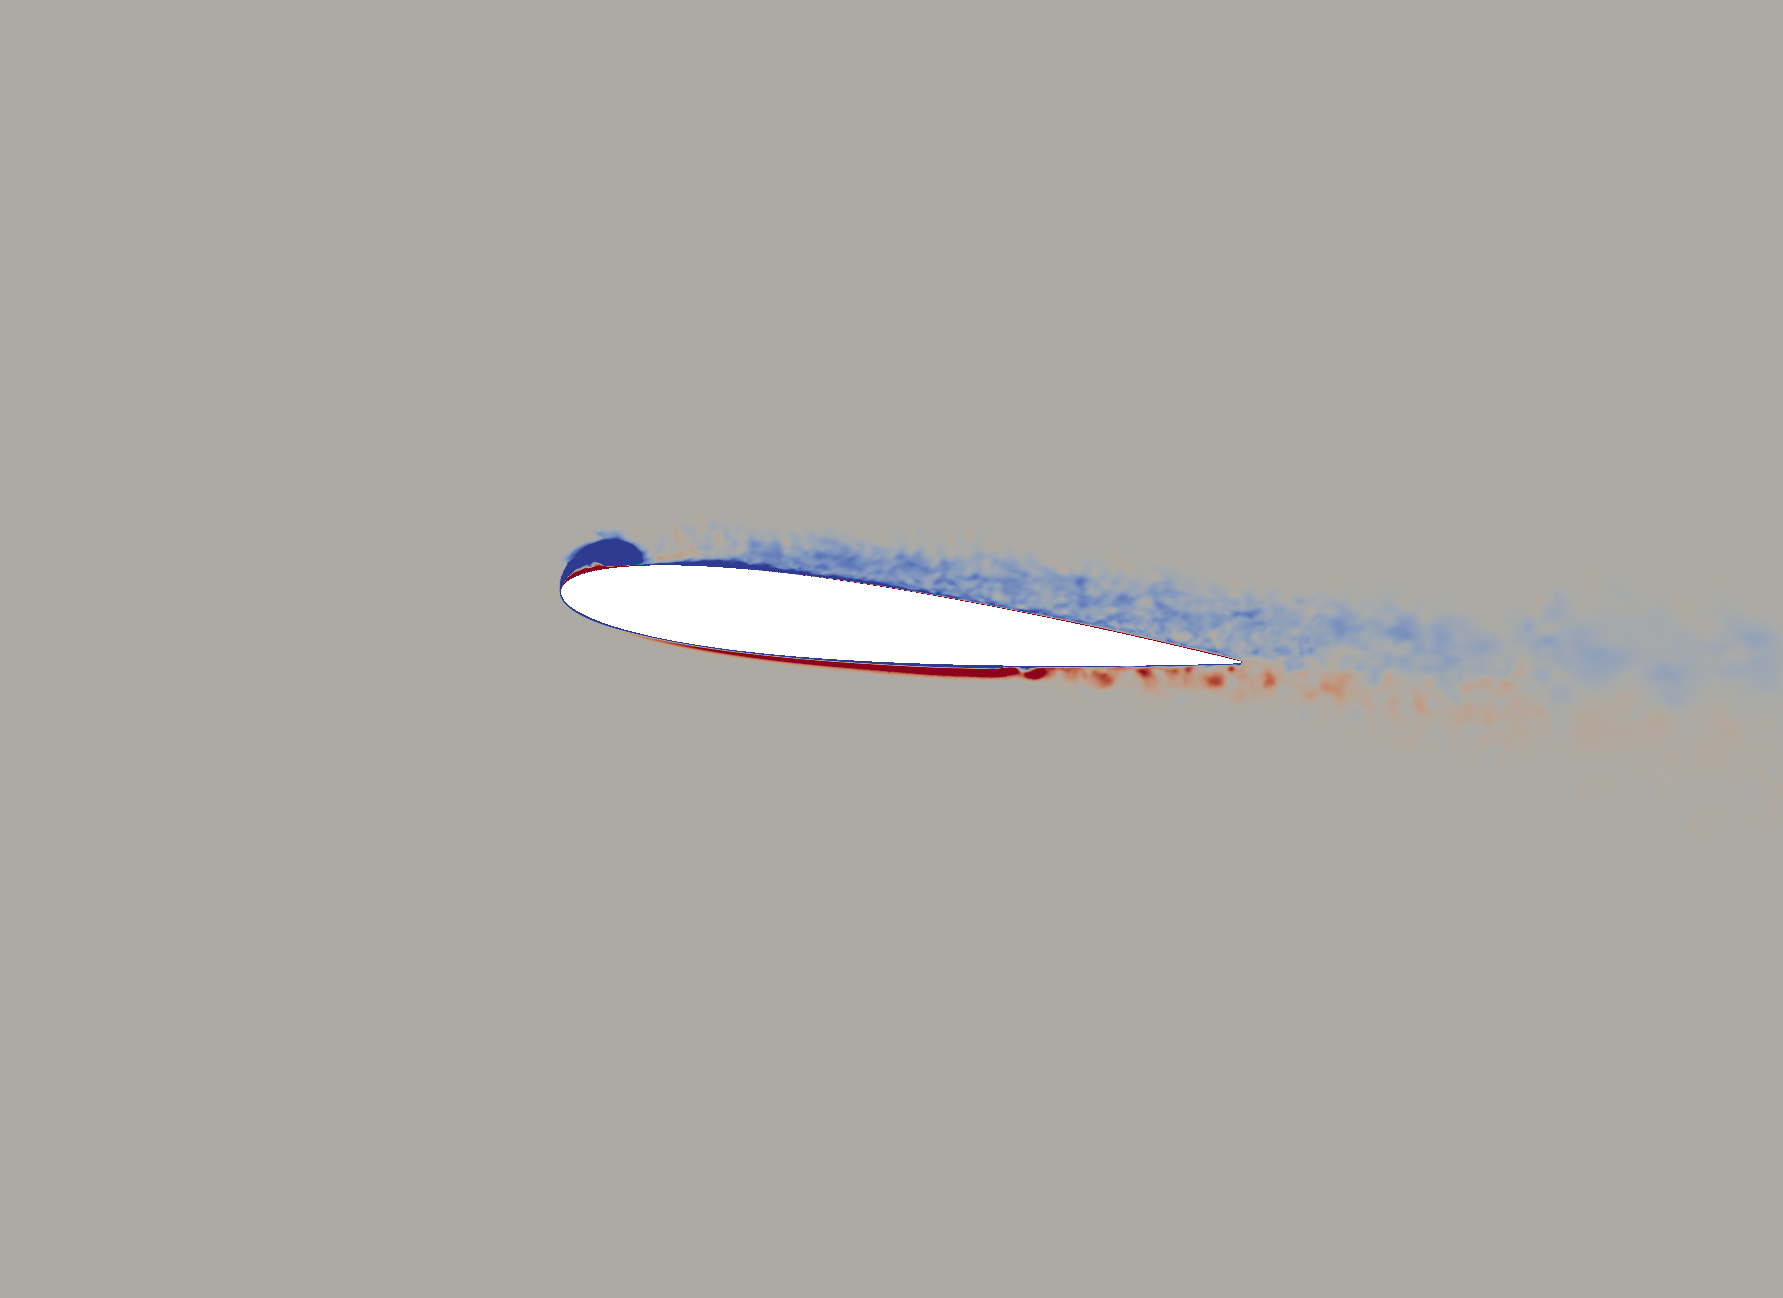
\includegraphics[width=1\textwidth]{figures/Vorticity_plots/Re_200k_1pt0/phase_240.png}
		\caption{$Re=2e5$, $\psi$ = $240^\circ$, $\tilde{t}=0.667$}
		\label{fig:Re_200k_1pt0_phi240}
	\end{subfigure}
	\begin{subfigure}[b]{0.32\textwidth}
		\centering
		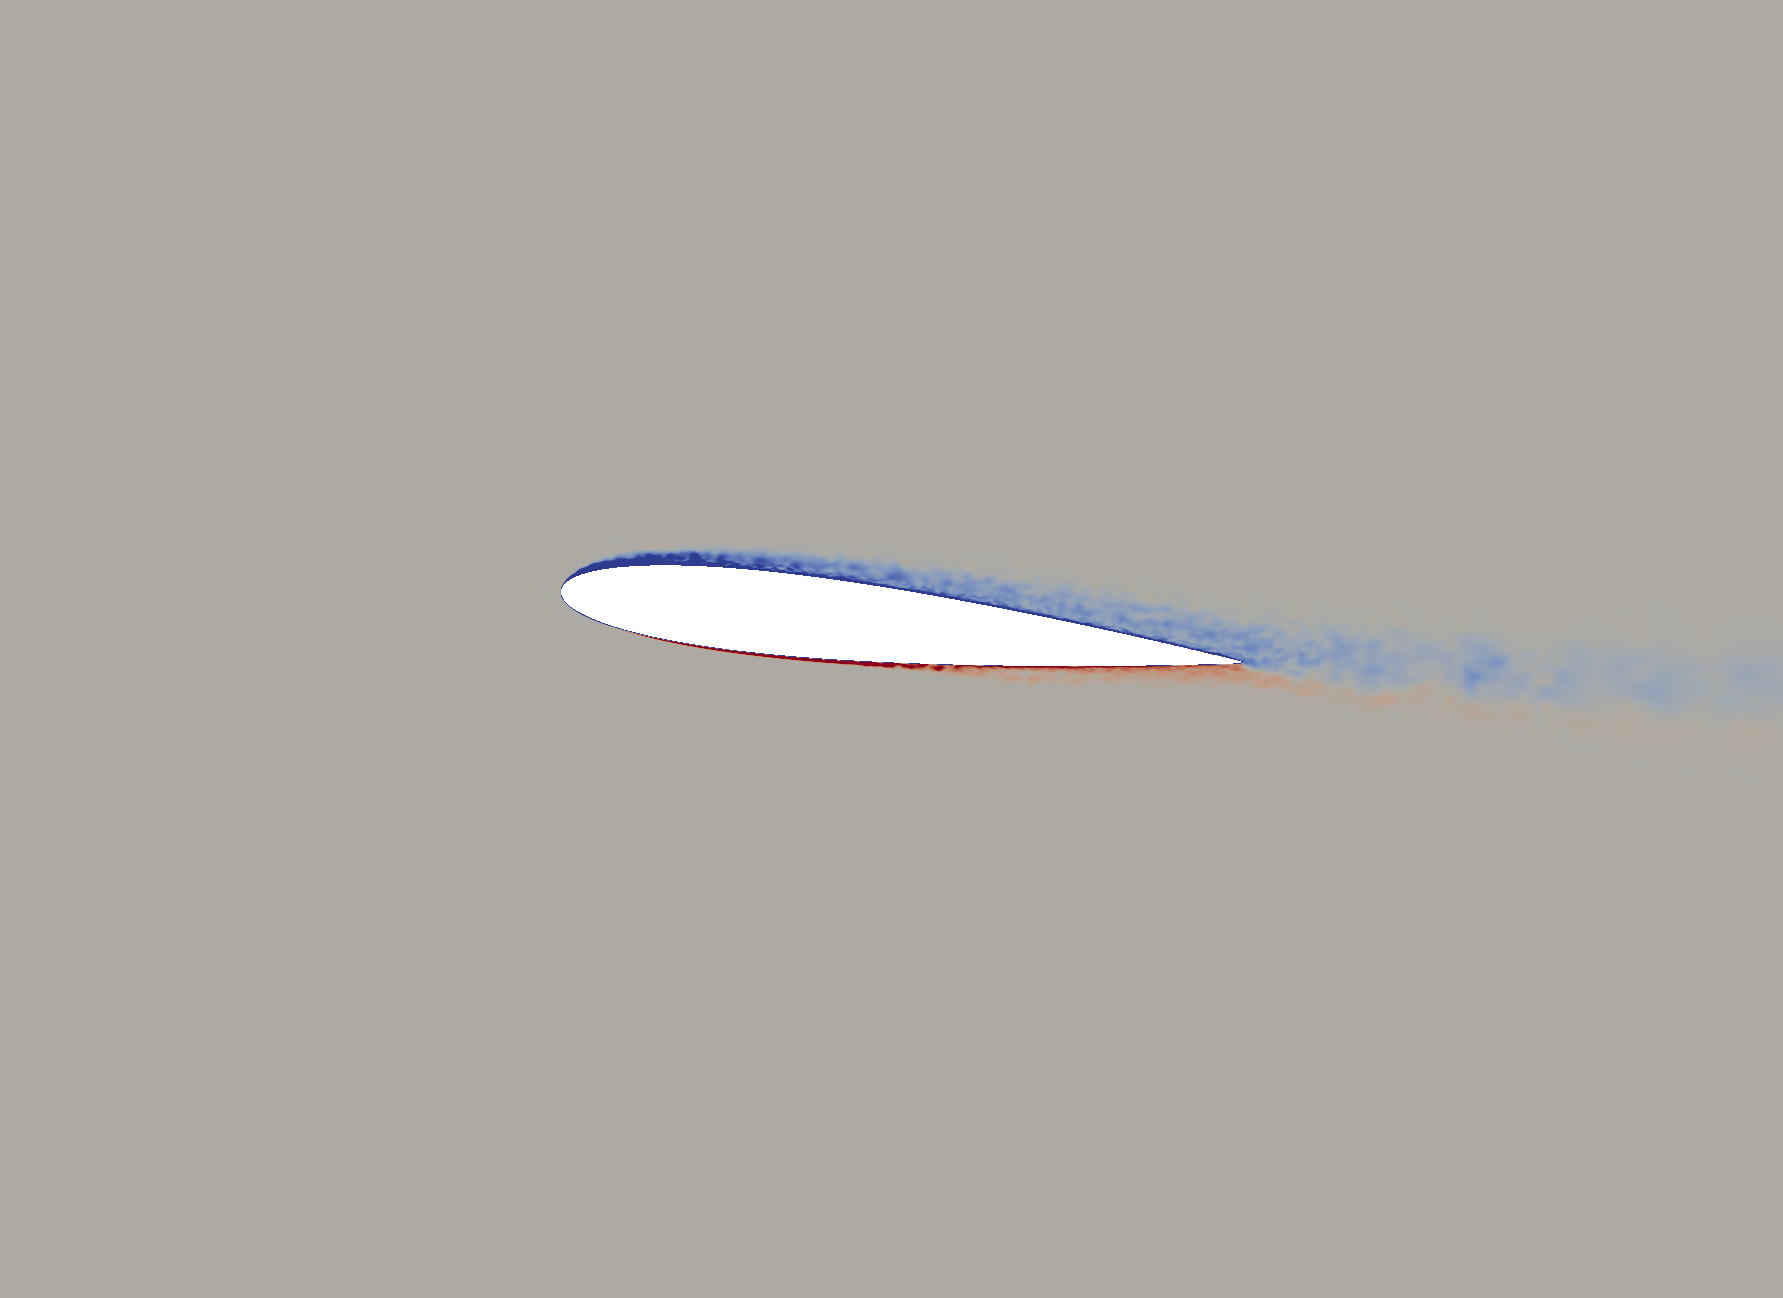
\includegraphics[width=1\textwidth]{figures/Vorticity_plots/Re_1m_1pt0/phase_240.png}
		\caption{$Re=1e6$, $\psi$ = $240^\circ$, $\tilde{t}=0.667$}
		\label{fig:Re_1m_1pt0_phi240}
	\end{subfigure}
	
	\begin{subfigure}[b]{0.32\textwidth}
		\centering
		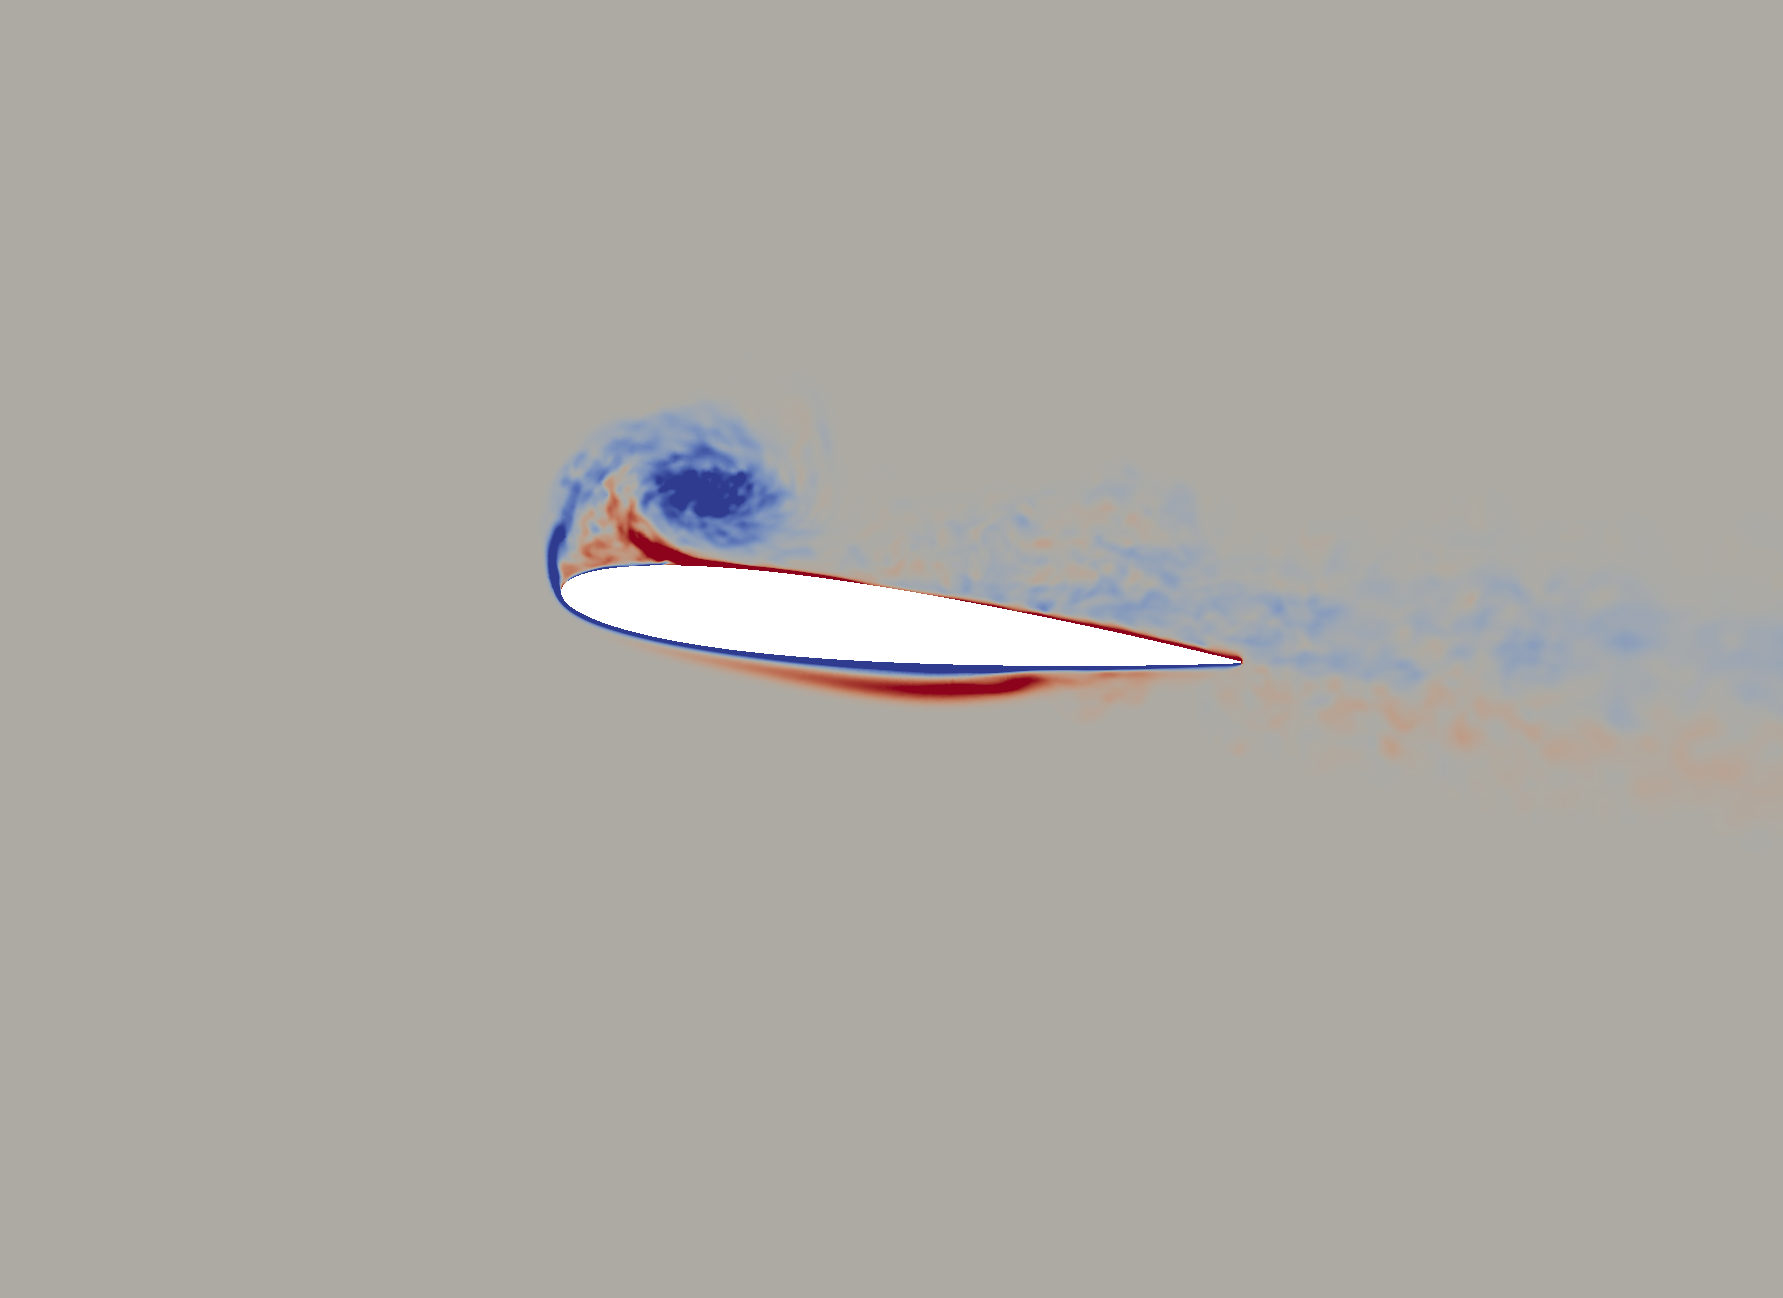
\includegraphics[width=1\textwidth]{figures/Vorticity_plots/Re_40k_1pt0/phase_255.png}
		\caption{$Re=4e4$, $\psi$ = $255^\circ$, $\tilde{t}=0.708$}
		\label{fig:Re_40k_1pt0_phi255}
	\end{subfigure}
	\begin{subfigure}[b]{0.32\textwidth}
		\centering
		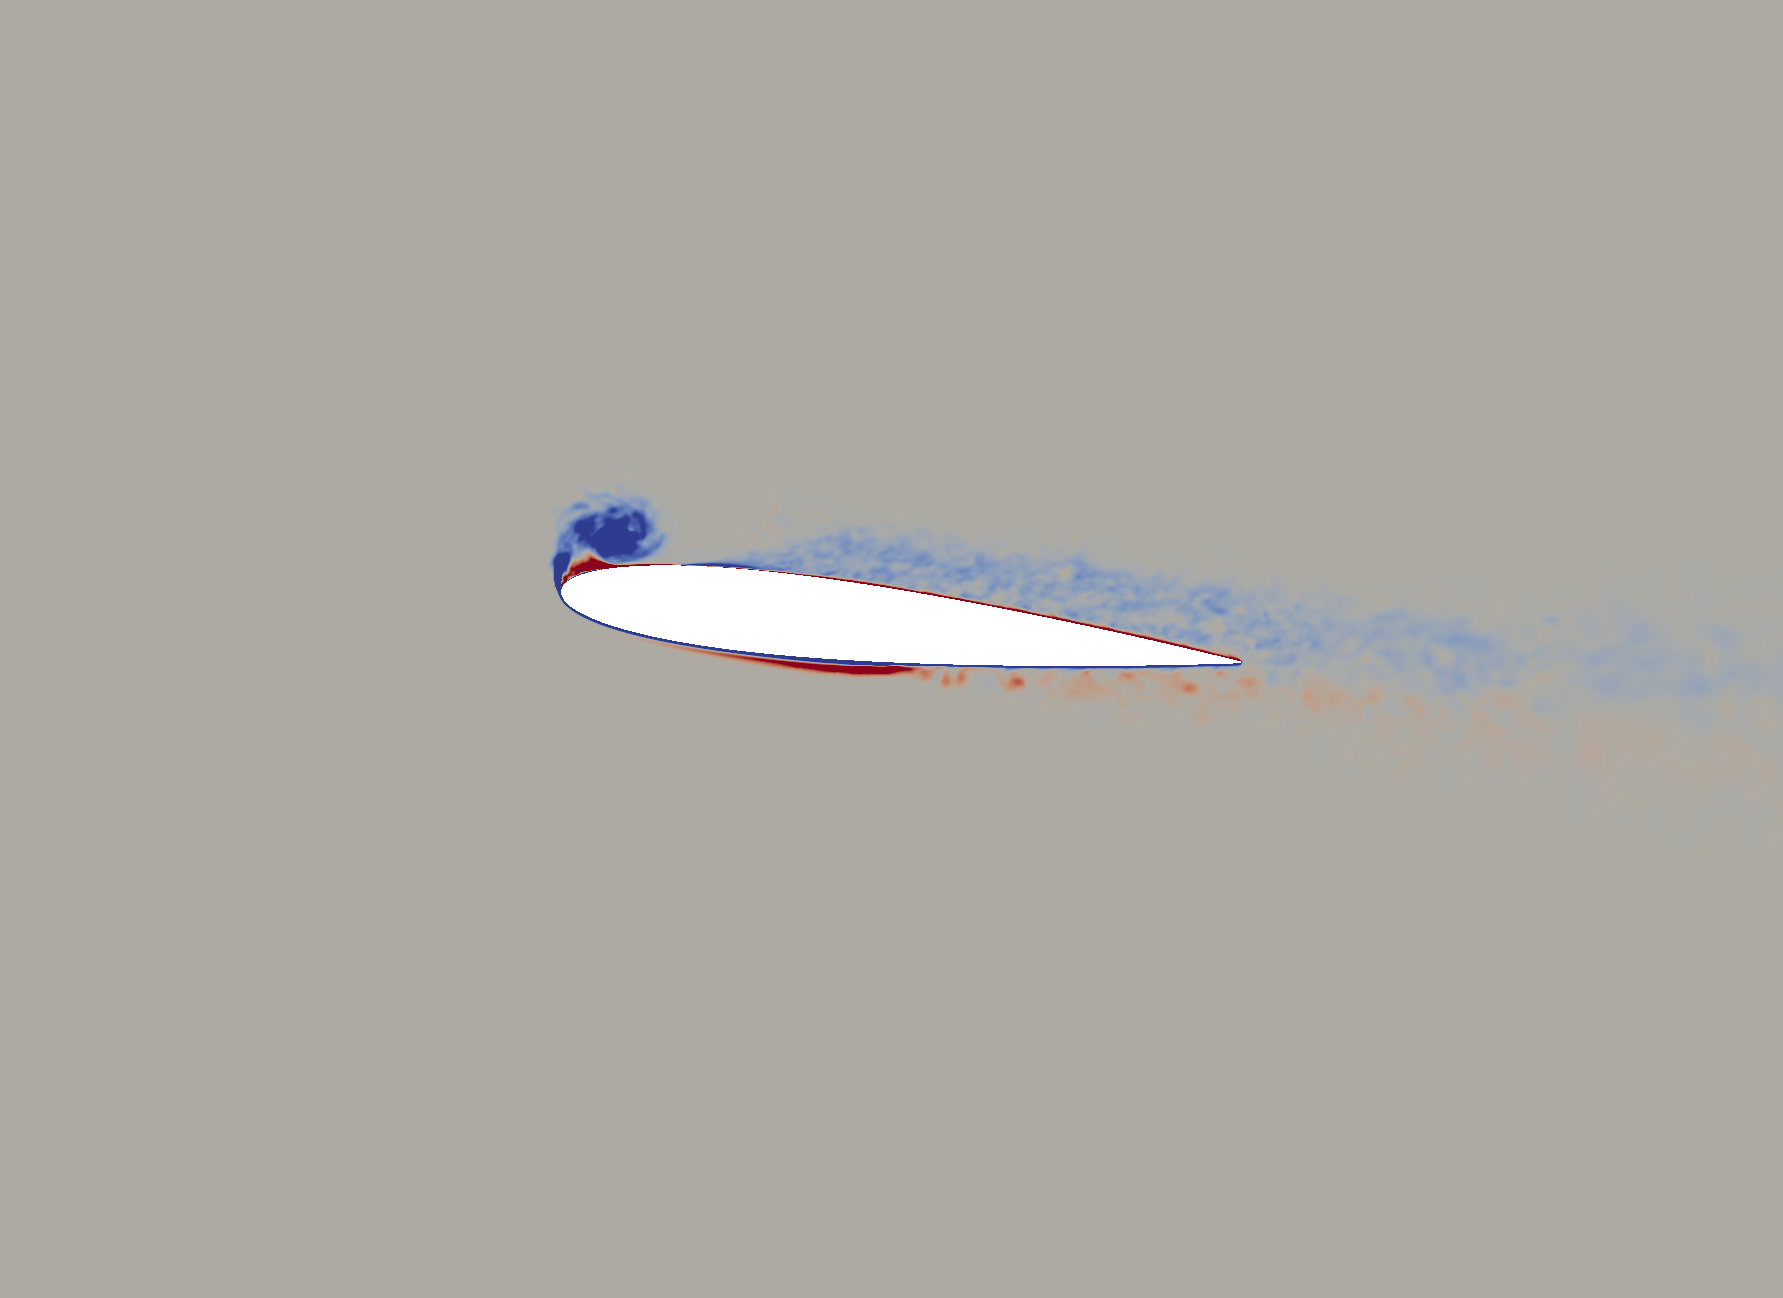
\includegraphics[width=1\textwidth]{figures/Vorticity_plots/Re_200k_1pt0/phase_255.png}
		\caption{$Re=2e5$, $\psi$ = $255^\circ$, $\tilde{t}=0.708$}
		\label{fig:Re_200k_1pt0_phi255}
	\end{subfigure}
	\begin{subfigure}[b]{0.32\textwidth}
		\centering
		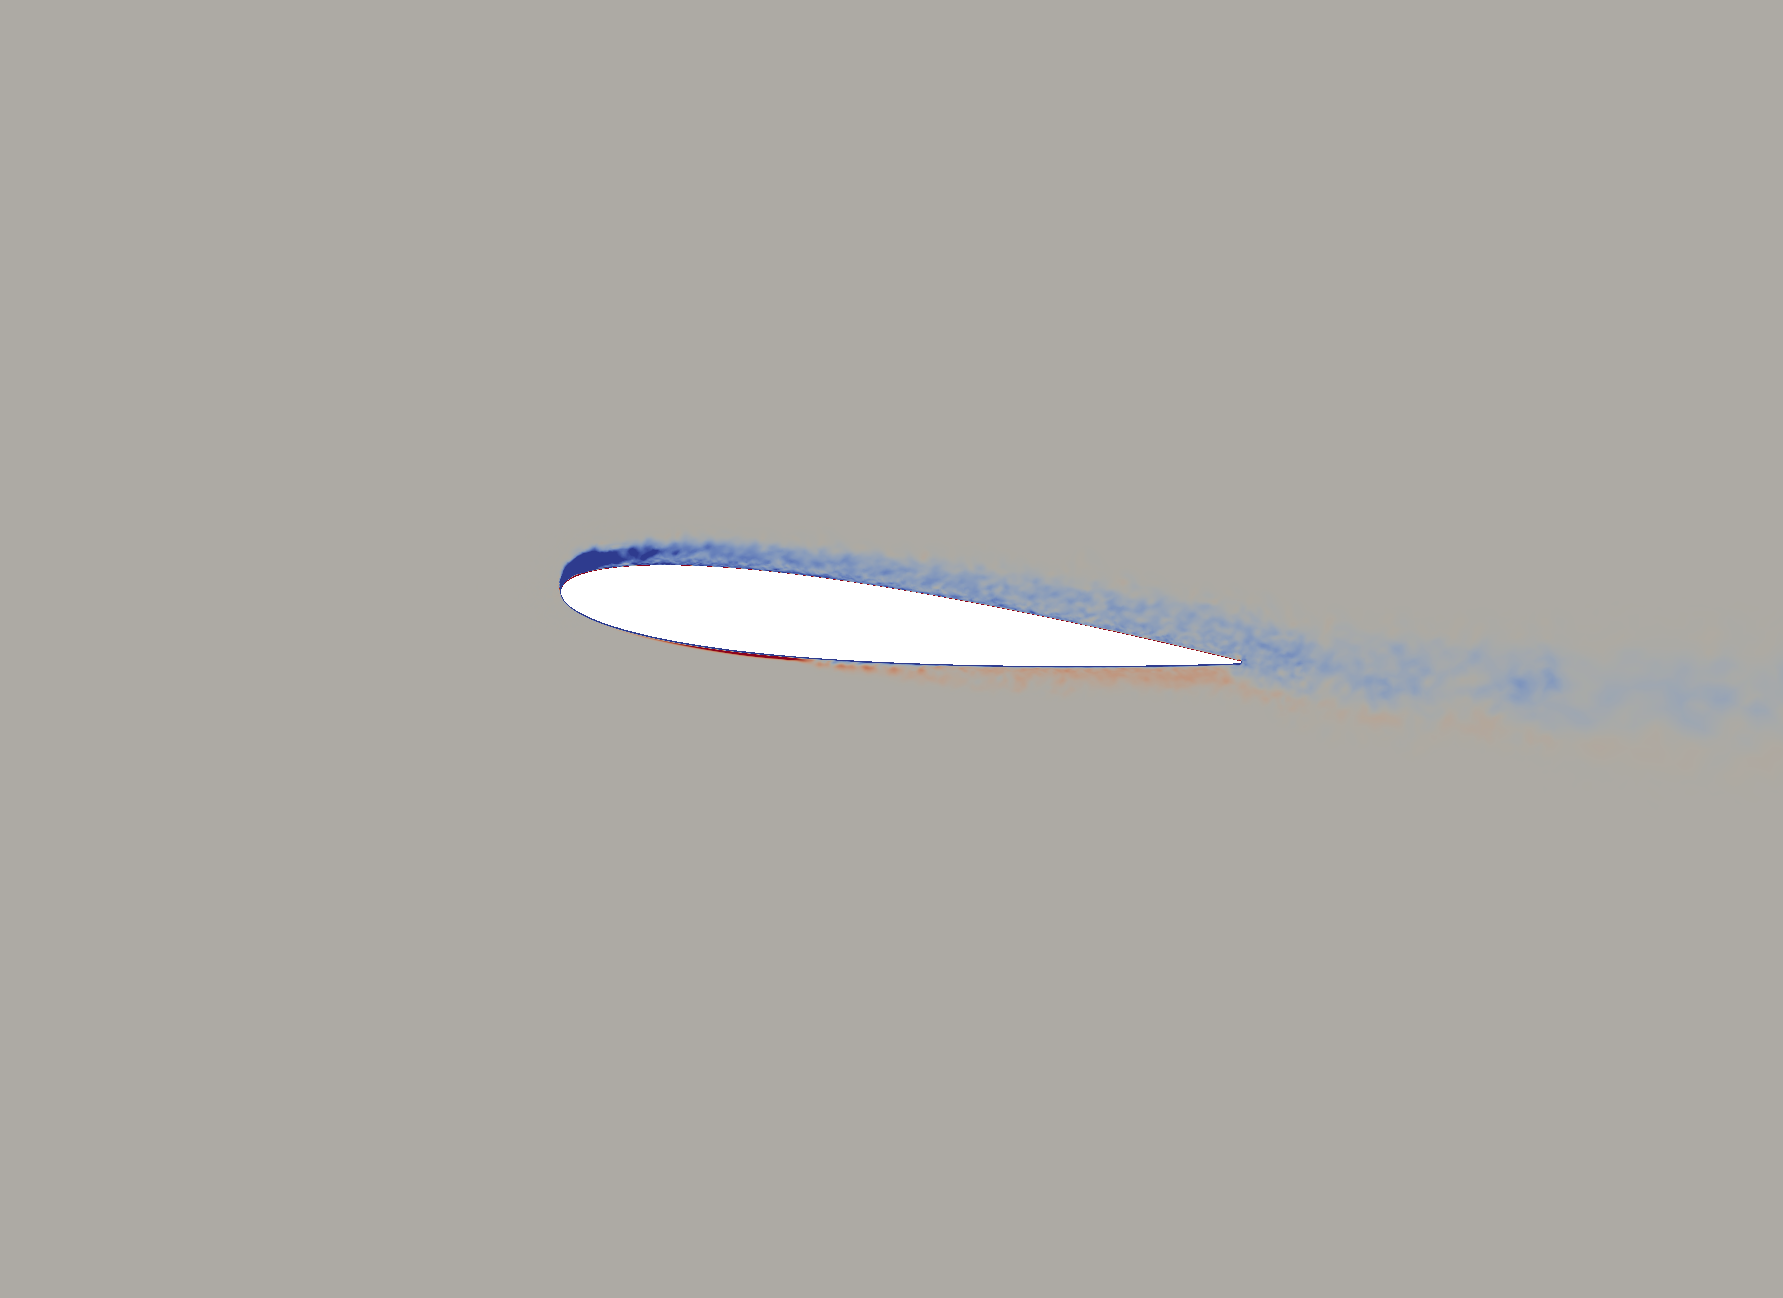
\includegraphics[width=1\textwidth]{figures/Vorticity_plots/Re_1m_1pt0/phase_255.png}
		\caption{$Re=1e6$, $\psi$ = $255^\circ$, $\tilde{t}=0.708$}
		\label{fig:Re_1m_1pt0_phi255}
	\end{subfigure}
	
	\caption{Spanwise vorticity at 8 different phases for $Re$=40,000 (left column), 200,000 (middle column) and 1,000,000 (right column) at $\mu_{sect}$ = 1.0}
	\label{fig:vortScreen_1pt0}
\end{figure}


\begin{figure}[H]\ContinuedFloat
	\centering
	\begin{subfigure}[b]{0.32\textwidth}
		\centering
		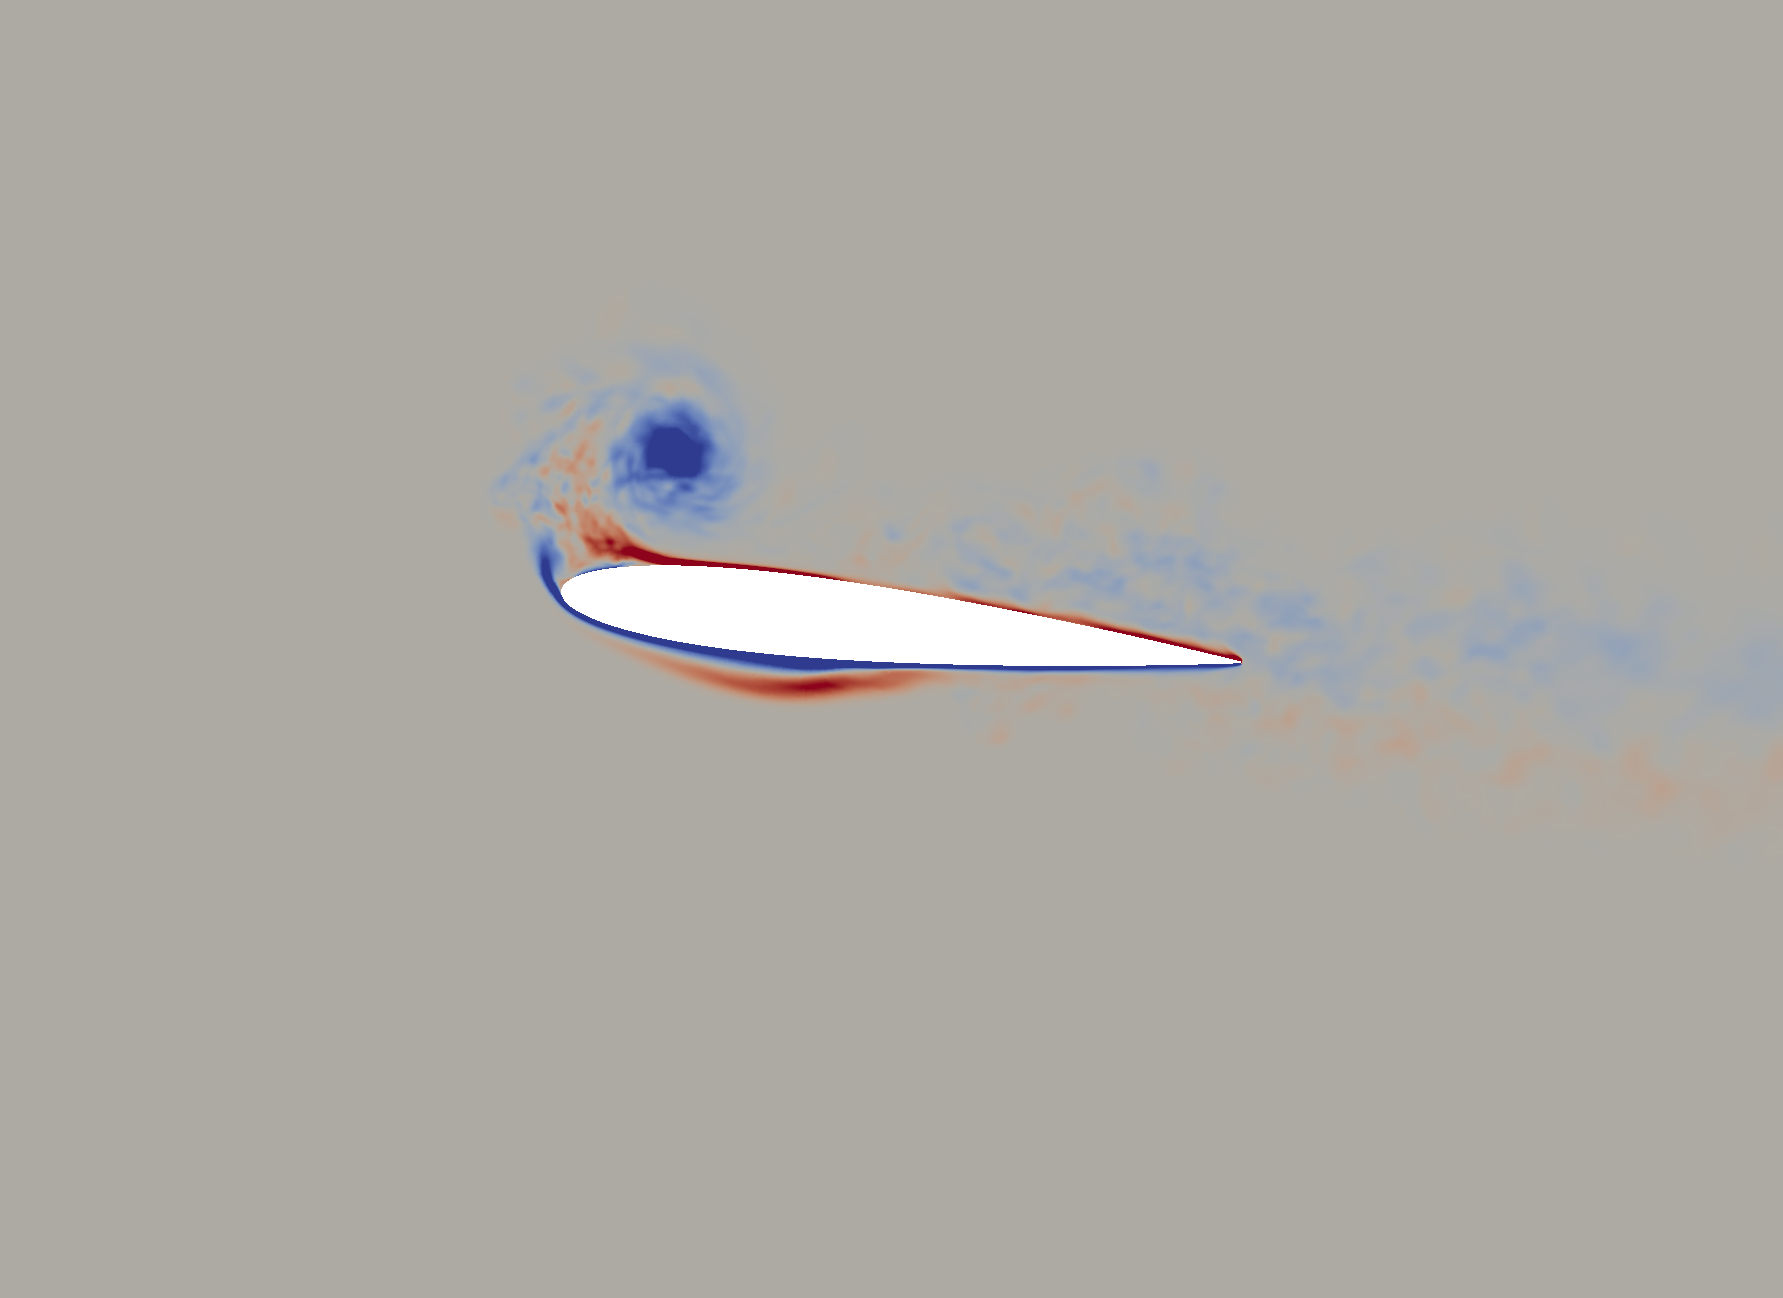
\includegraphics[width=1\textwidth]{figures/Vorticity_plots/Re_40k_1pt0/phase_270.png}
		\caption{$Re=4e4$, $\psi$ = $270^\circ$, $\tilde{t}=0.750$}
		\label{fig:Re_40k_1pt0_phi270}
	\end{subfigure}
	\begin{subfigure}[b]{0.32\textwidth}
		\centering
		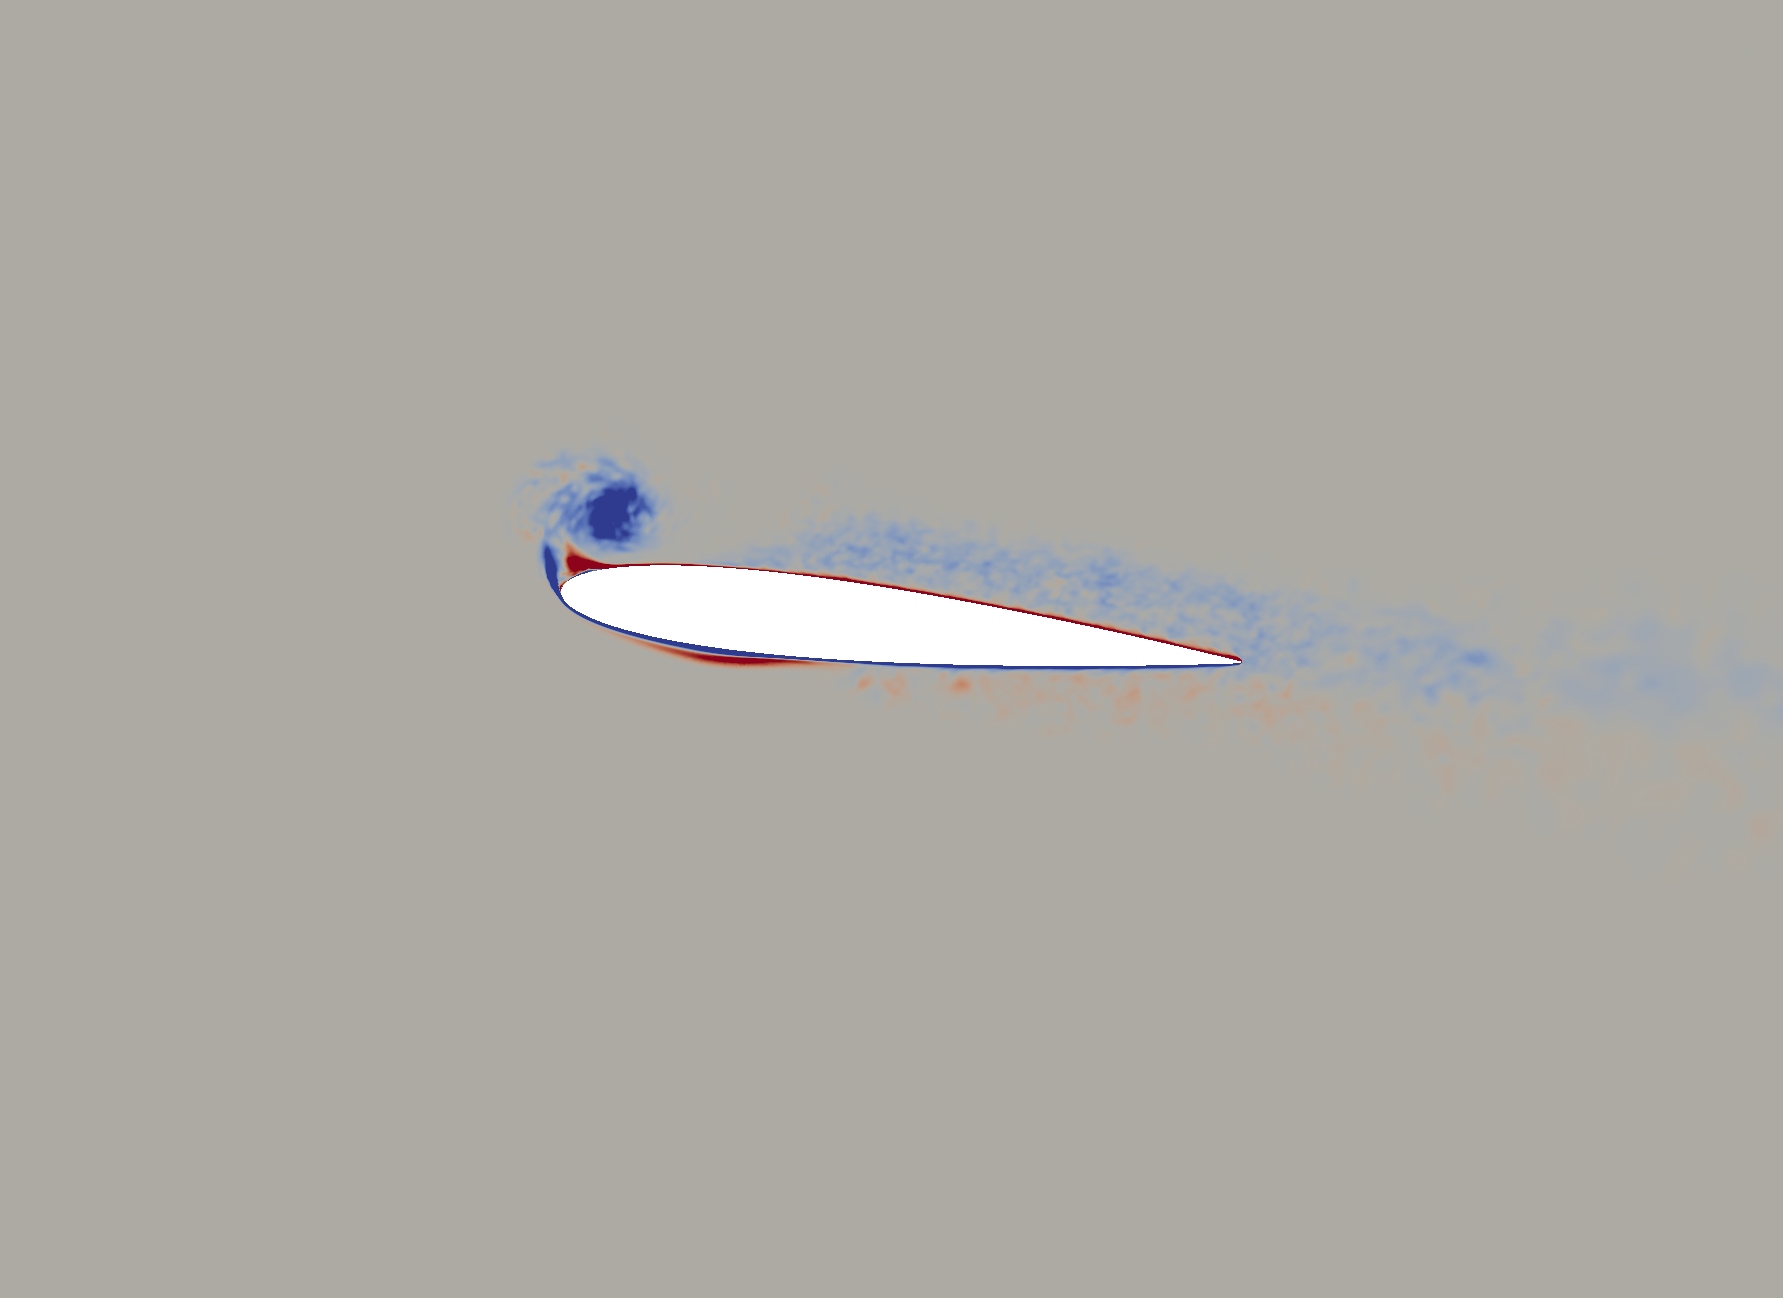
\includegraphics[width=1\textwidth]{figures/Vorticity_plots/Re_200k_1pt0/phase_270.png}
		\caption{$Re=2e5$, $\psi$ = $270^\circ$, $\tilde{t}=0.750$}
		\label{fig:Re_200k_1pt0_phi270}
	\end{subfigure}
	\begin{subfigure}[b]{0.32\textwidth}
		\centering
		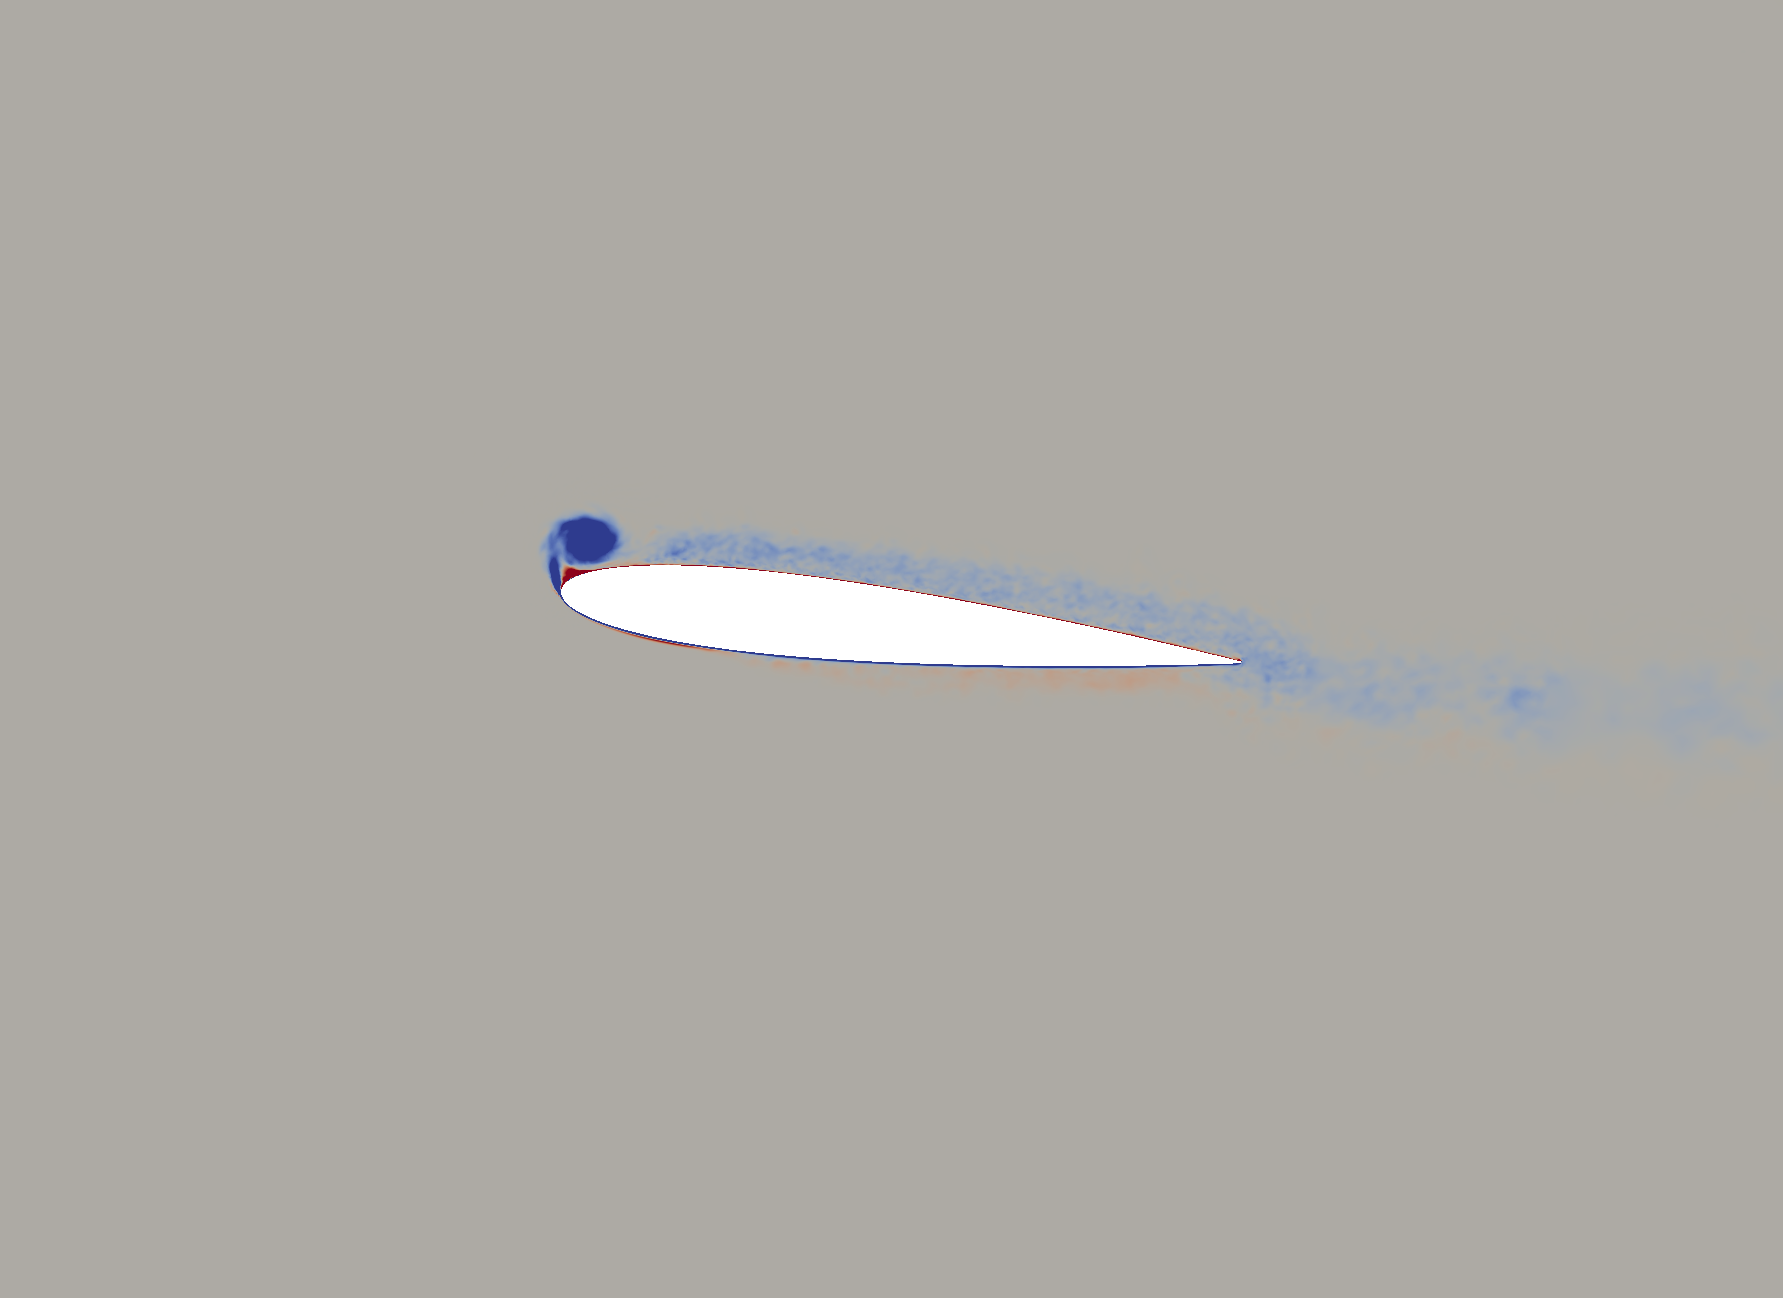
\includegraphics[width=1\textwidth]{figures/Vorticity_plots/Re_1m_1pt0/phase_270.png}
		\caption{$Re=1e6$, $\psi$ = $270^\circ$, $\tilde{t}=0.750$}
		\label{fig:Re_1m_1pt0_phi270}
	\end{subfigure}
	
	\begin{subfigure}[b]{0.32\textwidth}
		\centering
		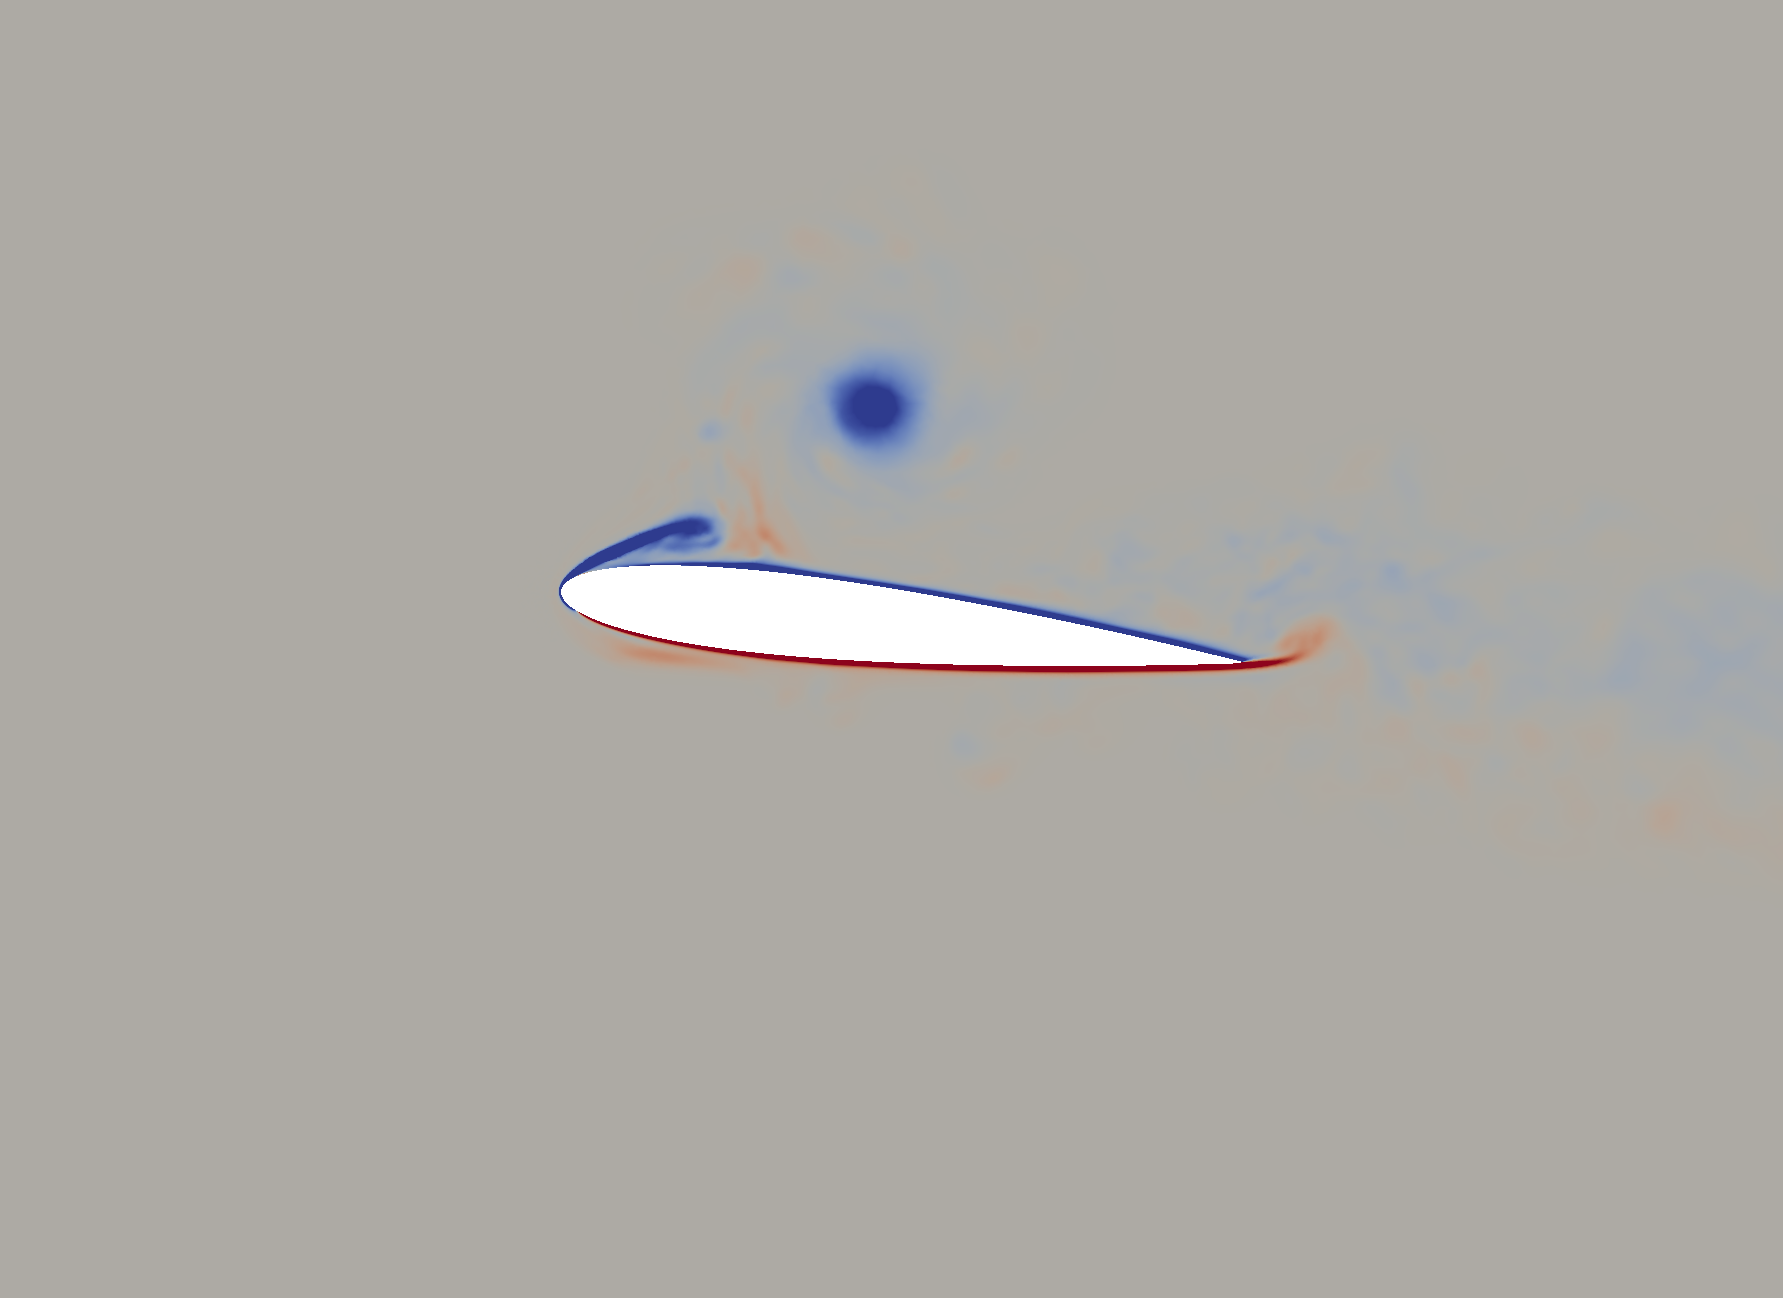
\includegraphics[width=1\textwidth]{figures/Vorticity_plots/Re_40k_1pt0/phase_315.png}
		\caption{$Re=4e4$, $\psi$ = $315^\circ$, $\tilde{t}=0.875$}
		\label{fig:Re_40k_1pt0_phi315}
	\end{subfigure}
	\begin{subfigure}[b]{0.32\textwidth}
		\centering
		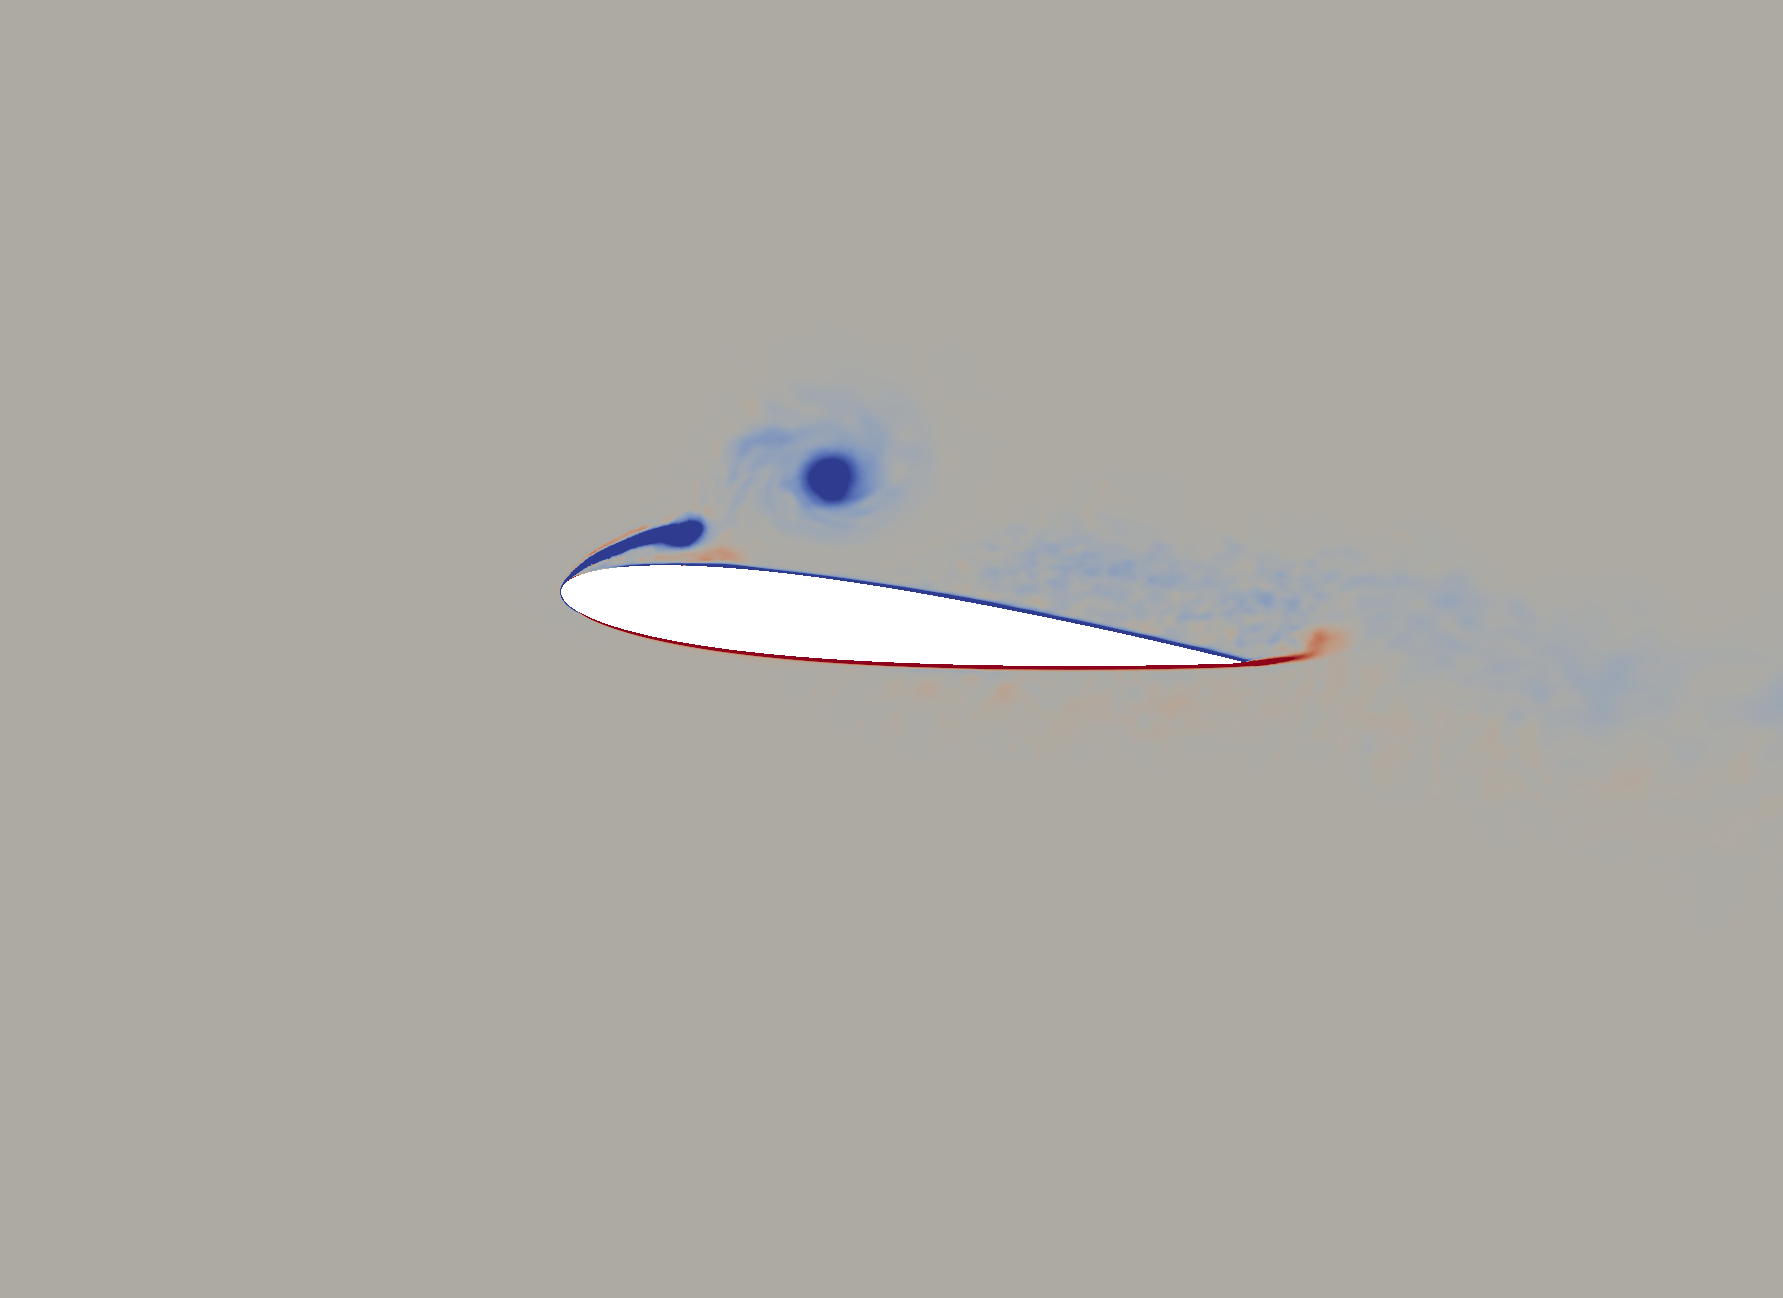
\includegraphics[width=1\textwidth]{figures/Vorticity_plots/Re_200k_1pt0/phase_315.png}
		\caption{$Re=2e5$, $\psi$ = $315^\circ$, $\tilde{t}=0.875$}
		\label{fig:Re_200k_1pt0_phi315}
	\end{subfigure}
	\begin{subfigure}[b]{0.32\textwidth}
		\centering
		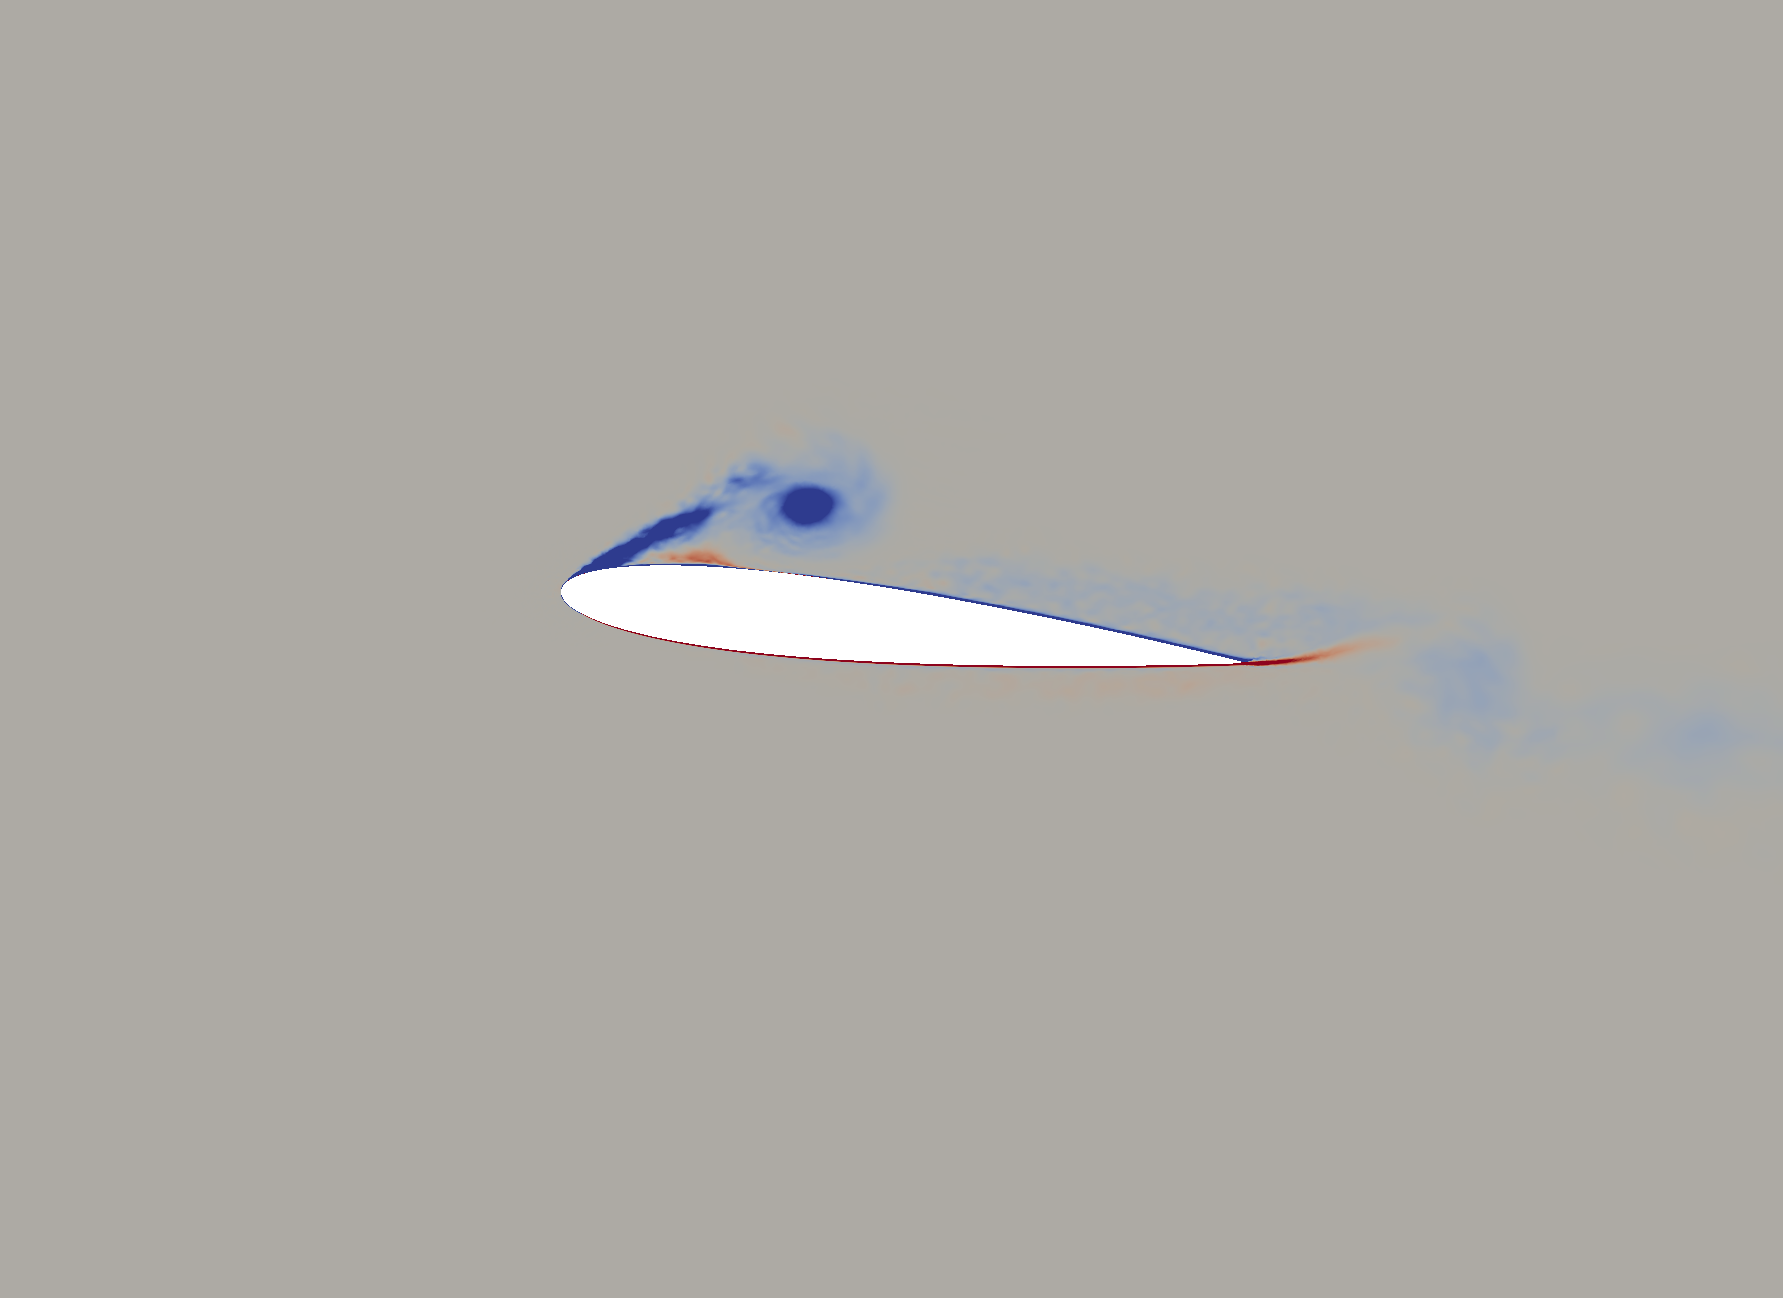
\includegraphics[width=1\textwidth]{figures/Vorticity_plots/Re_1m_1pt0/phase_315.png}
		\caption{$Re=1e6$, $\psi$ = $315^\circ$, $\tilde{t}=0.875$}
		\label{fig:Re_1m_1pt0_phi315}
	\end{subfigure}
	
	\begin{subfigure}[b]{0.32\textwidth}
		\centering
		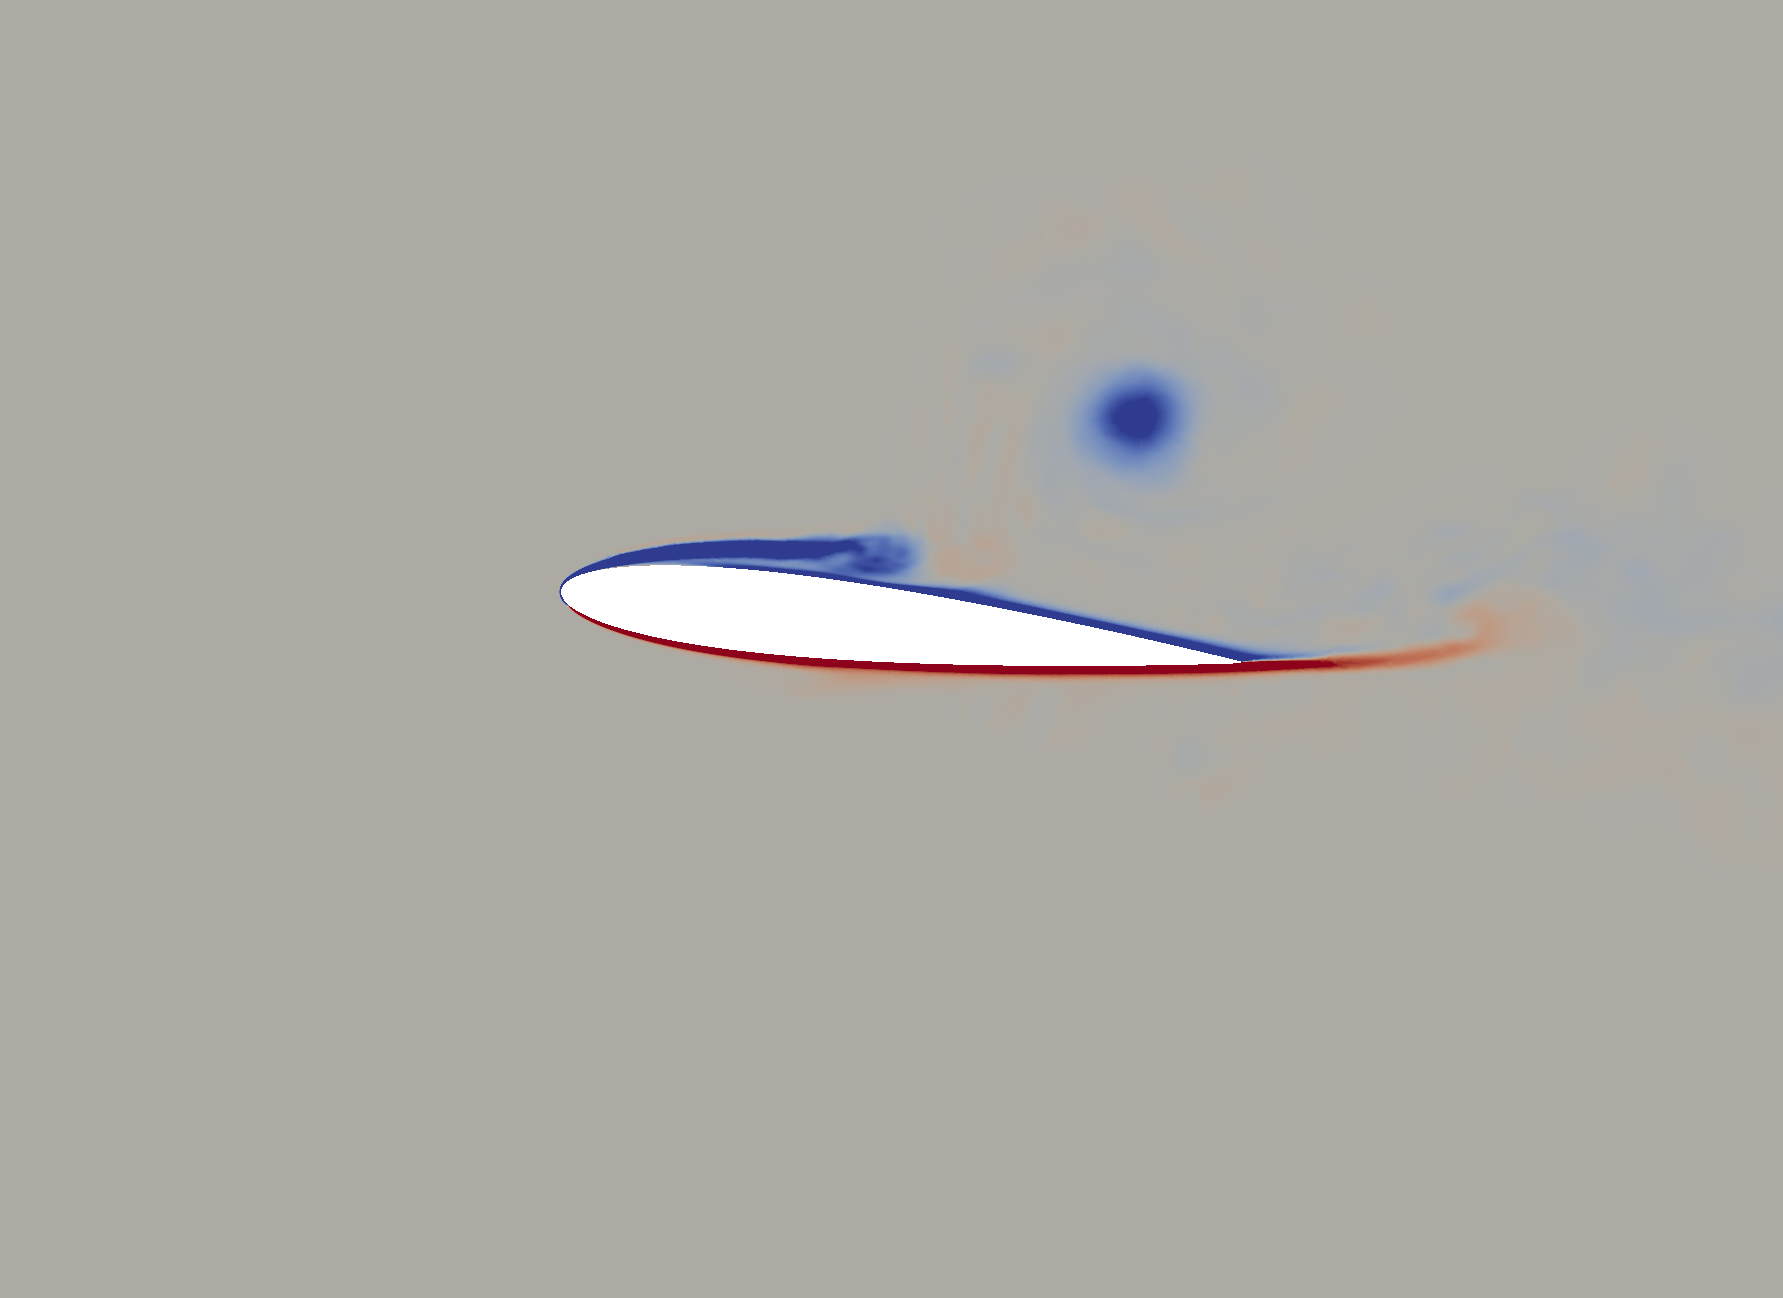
\includegraphics[width=1\textwidth]{figures/Vorticity_plots/Re_40k_1pt0/phase_330.png}
		\caption{$Re=4e4$, $\psi$ = $330^\circ$, $\tilde{t}=0.917$}
		\label{fig:Re_40k_1pt0_phi330}
	\end{subfigure}
	\begin{subfigure}[b]{0.32\textwidth}
		\centering
		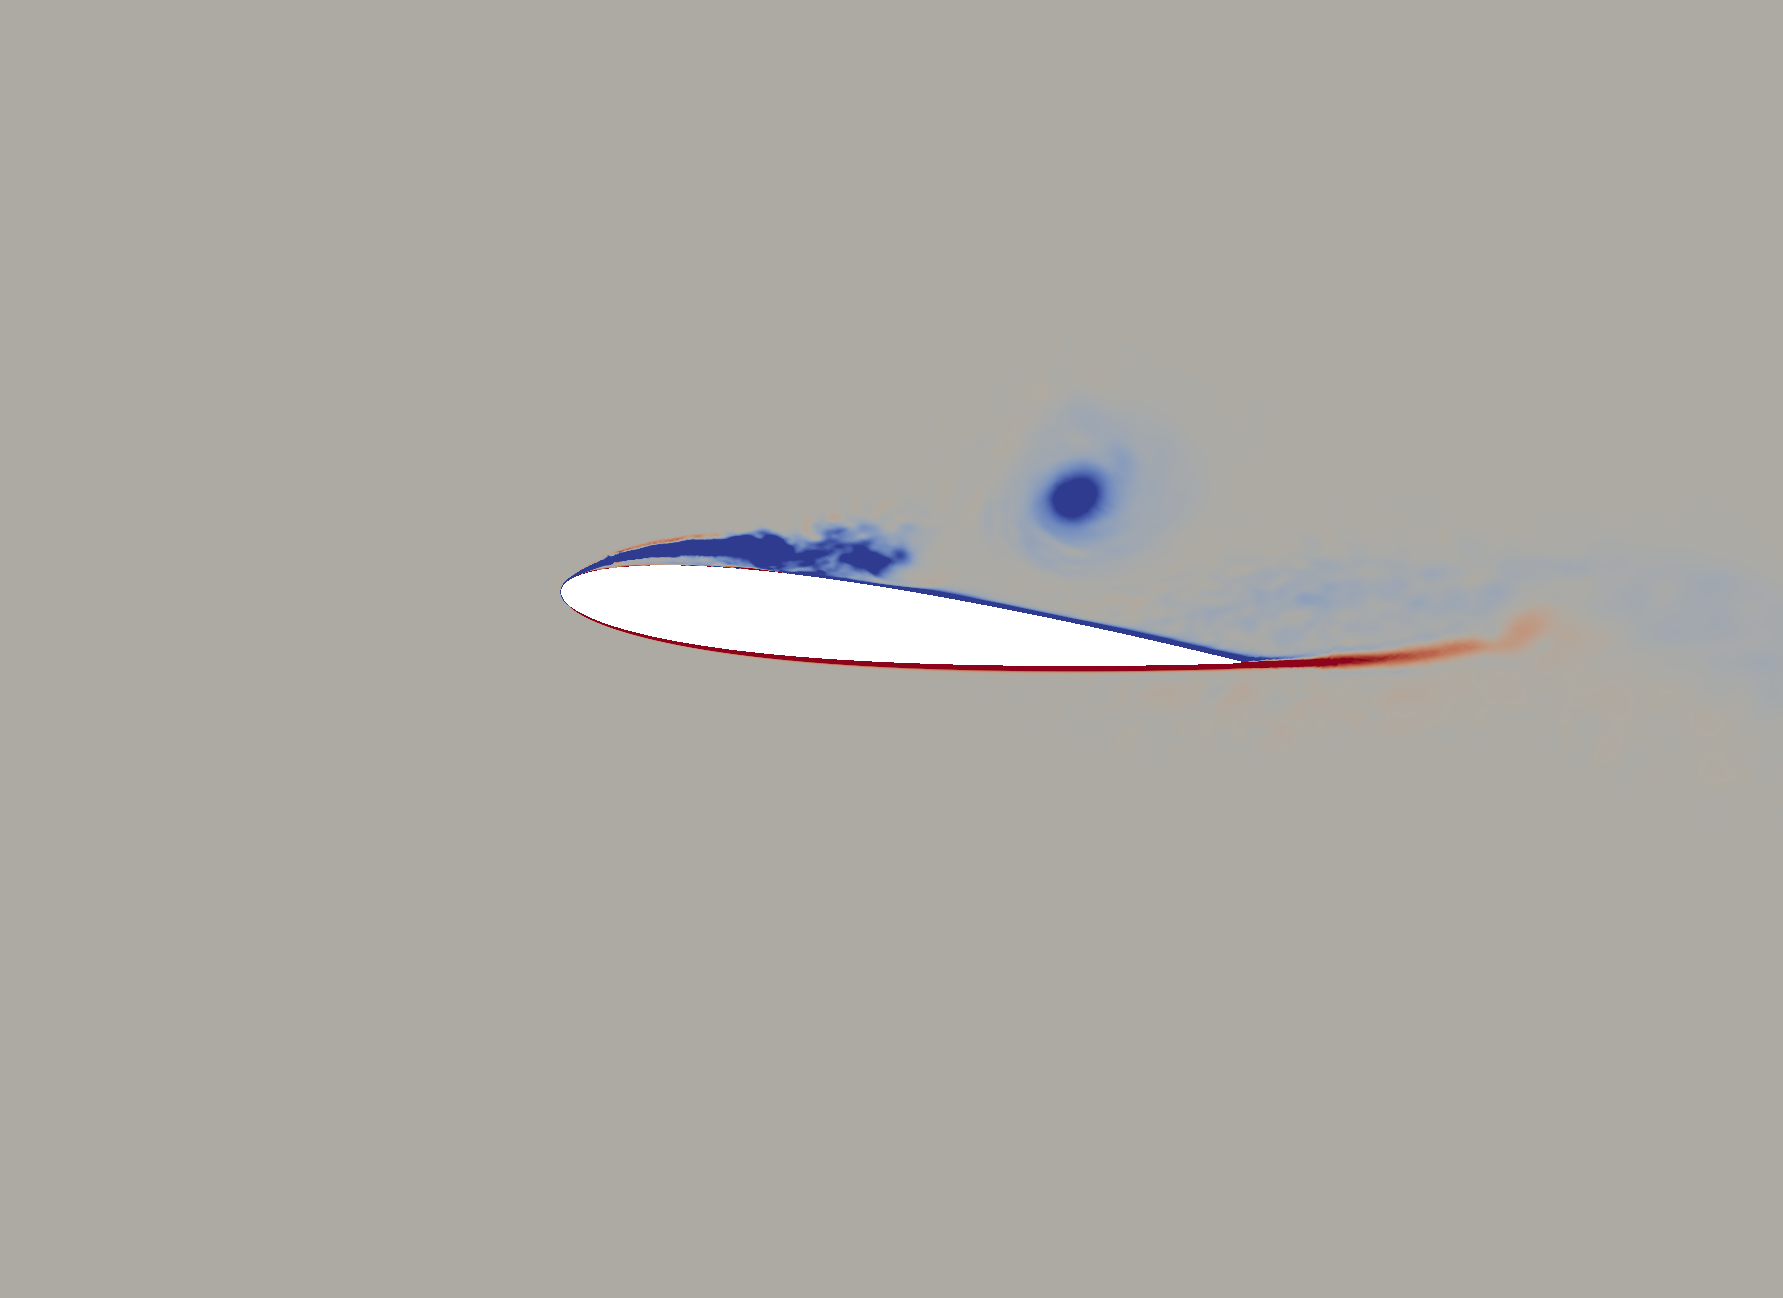
\includegraphics[width=1\textwidth]{figures/Vorticity_plots/Re_200k_1pt0/phase_330.png}
		\caption{$Re=2e5$, $\psi$ = $330^\circ$, $\tilde{t}=0.917$}
		\label{fig:Re_200k_1pt0_phi330}
	\end{subfigure}
	\begin{subfigure}[b]{0.32\textwidth}
		\centering
		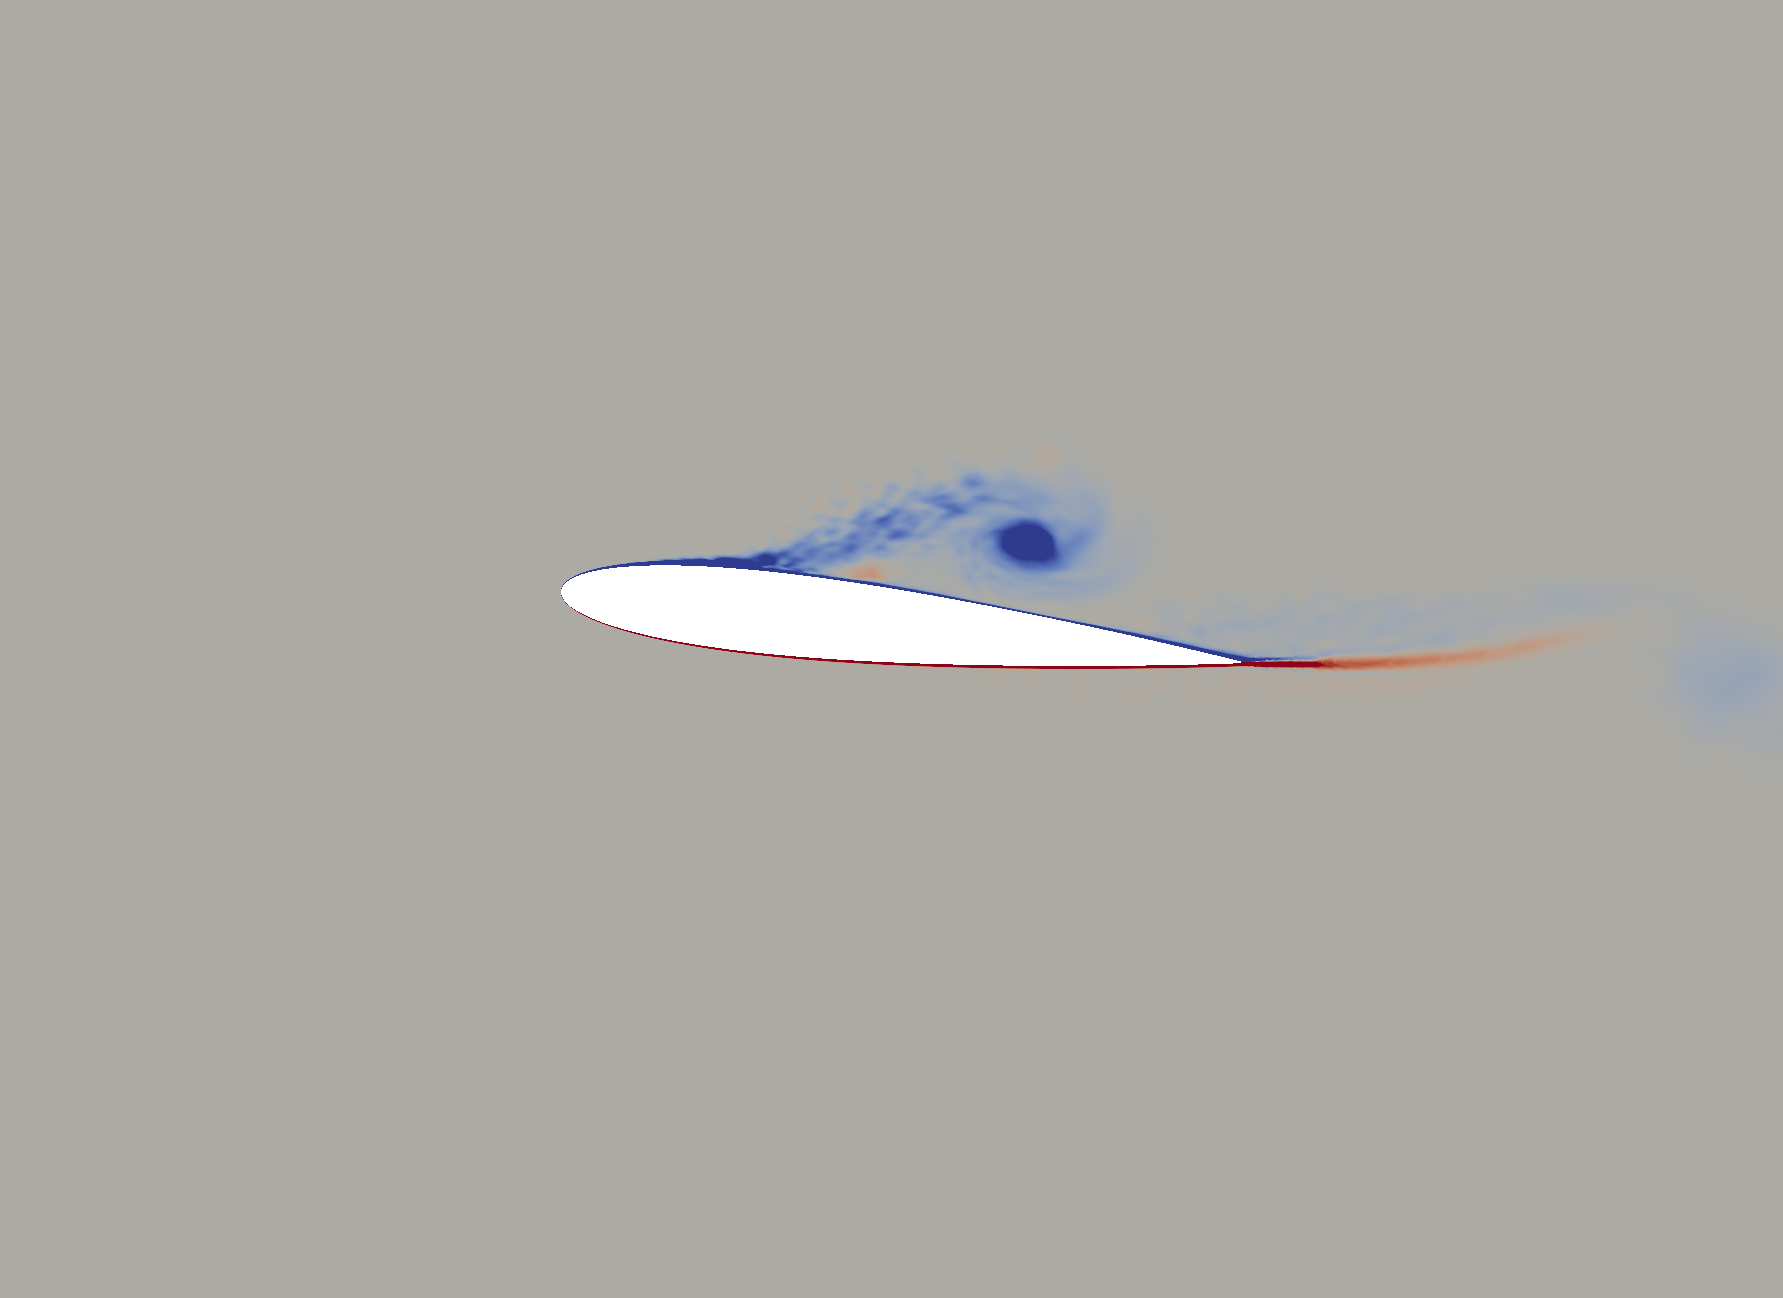
\includegraphics[width=1\textwidth]{figures/Vorticity_plots/Re_1m_1pt0/phase_330.png}
		\caption{$Re=1e6$,$\psi$ = $330^\circ$, $\tilde{t}=0.917$}
		\label{fig:Re_1m_1pt0_phi330}
	\end{subfigure}
	
	\begin{subfigure}[b]{0.32\textwidth}
		\centering
		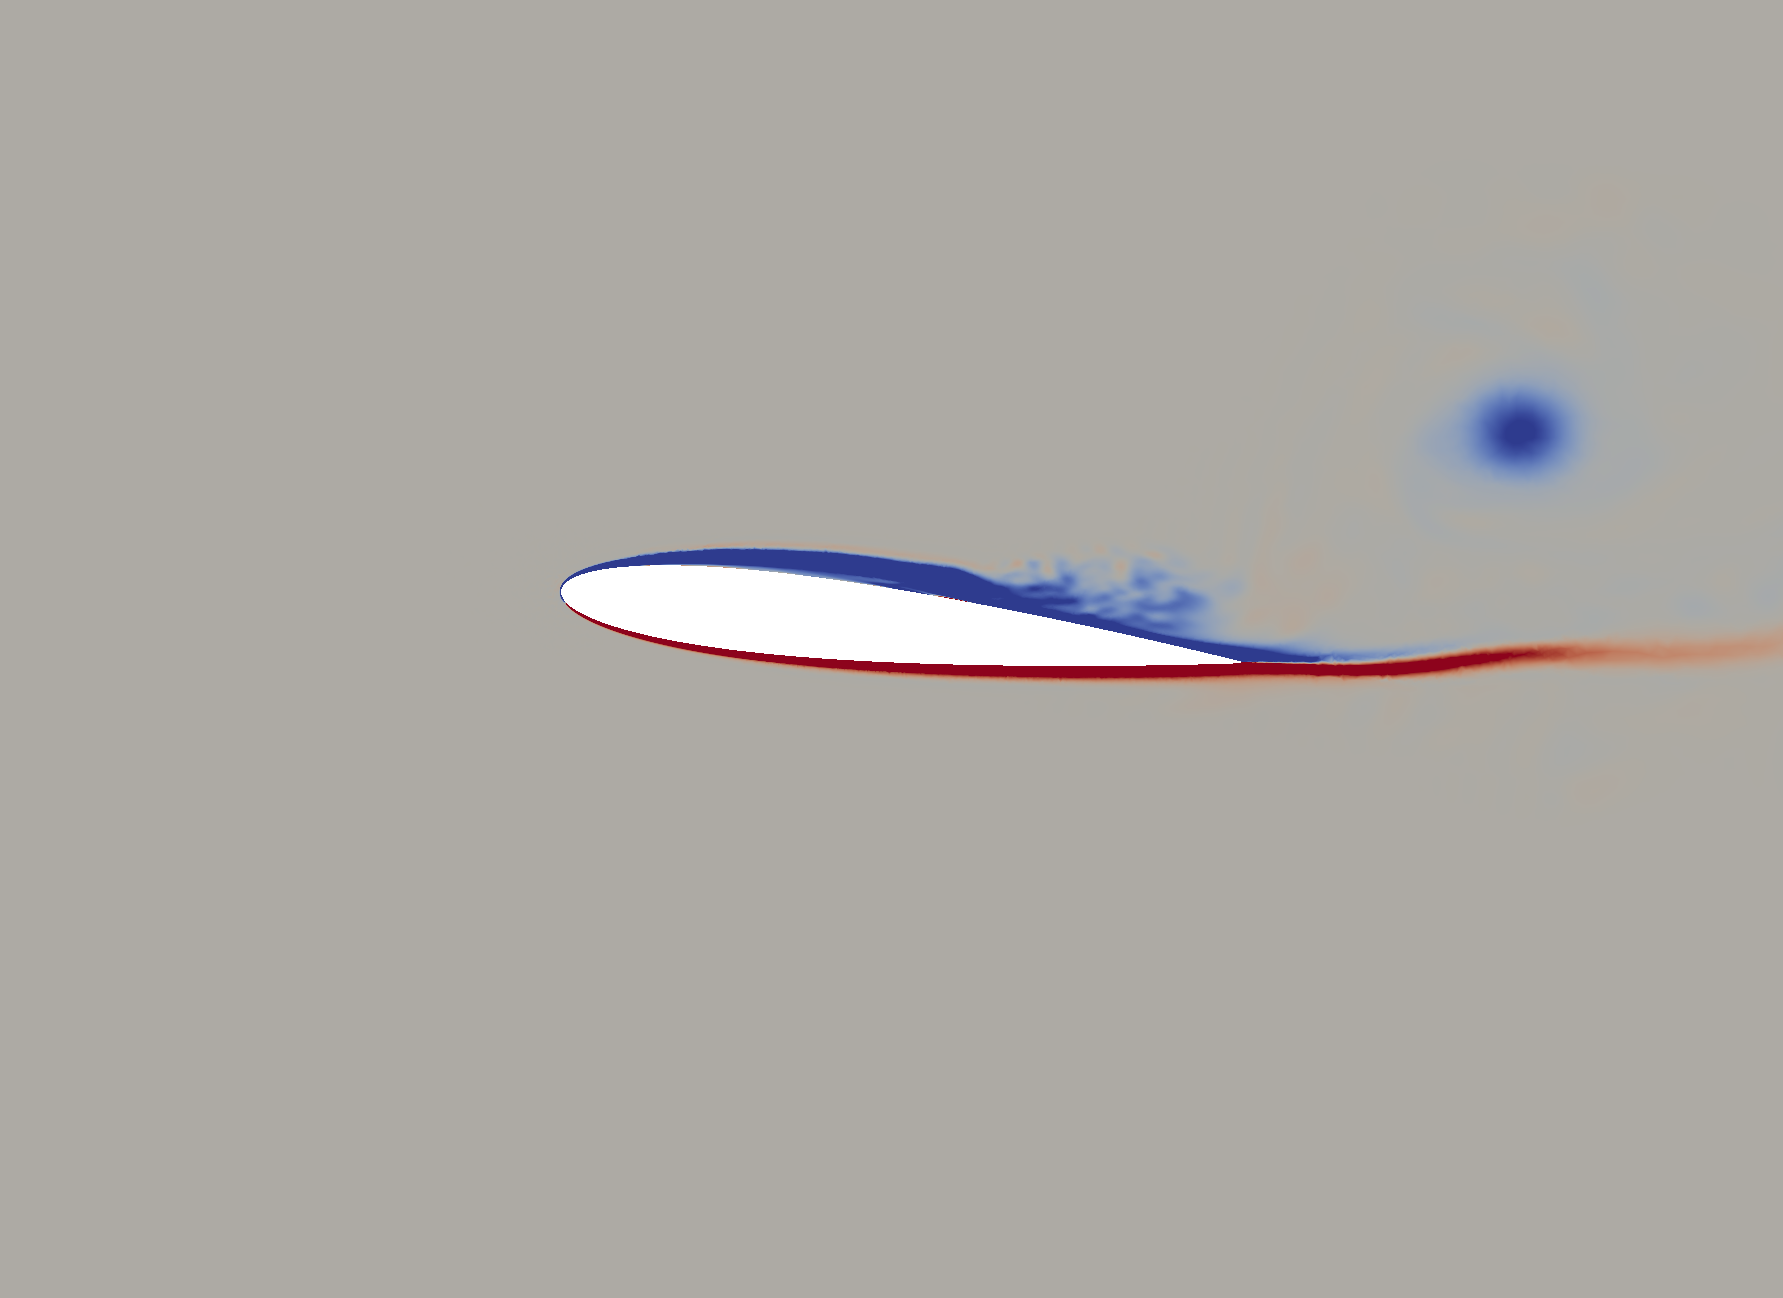
\includegraphics[width=1\textwidth]{figures/Vorticity_plots/Re_40k_1pt0/phase_345.png}
		\caption{$Re=4e4$, $\psi$ = $345^\circ$, $\tilde{t}=0.958$}
		\label{fig:Re_40k_1pt0_phi345}
	\end{subfigure}
	\begin{subfigure}[b]{0.32\textwidth}
		\centering
		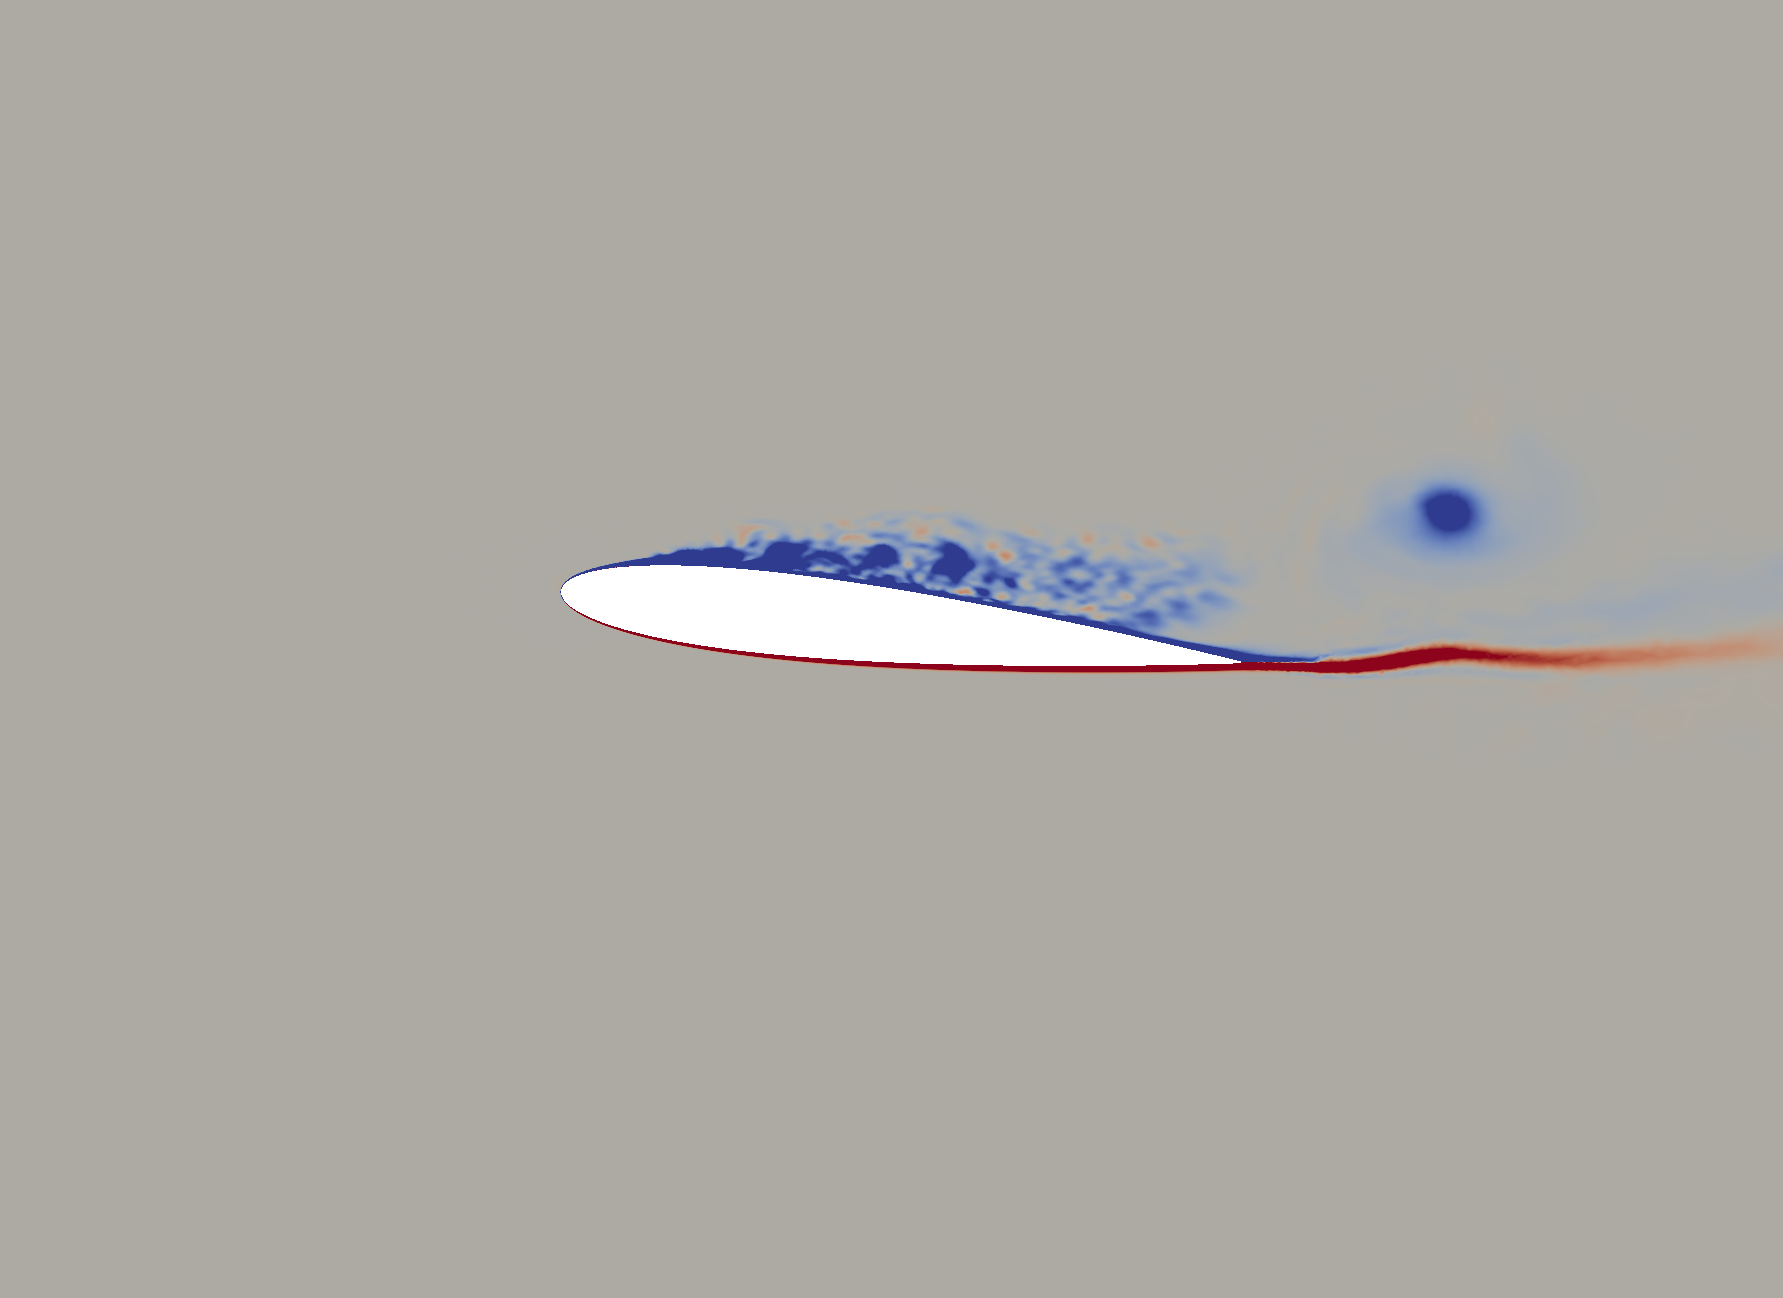
\includegraphics[width=1\textwidth]{figures/Vorticity_plots/Re_200k_1pt0/phase_345.png}
		\caption{$Re=2e5$, $\psi$ = $345^\circ$, $\tilde{t}=0.958$}
		\label{fig:Re_200k_1pt0_phi345}
	\end{subfigure}
	\begin{subfigure}[b]{0.32\textwidth}
		\centering
		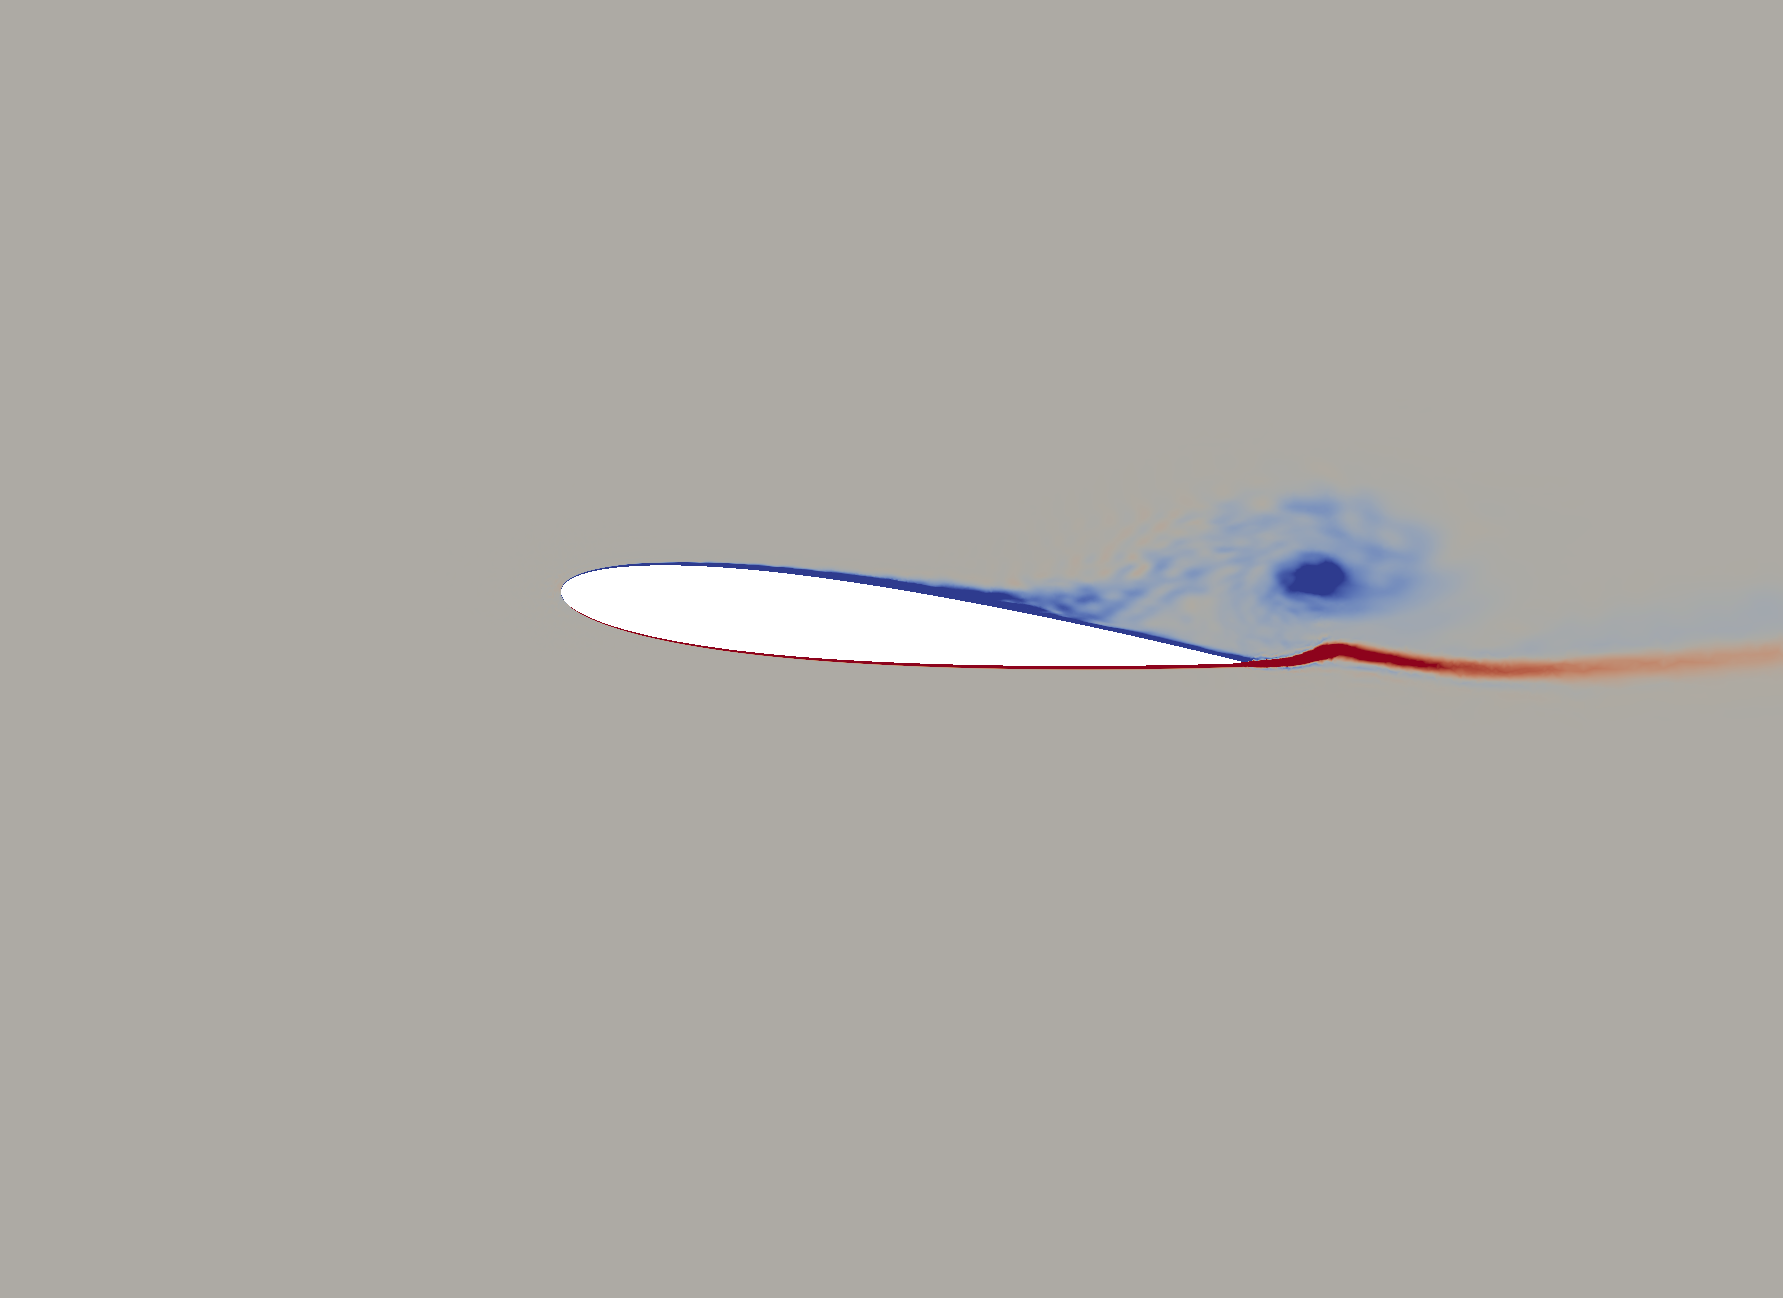
\includegraphics[width=1\textwidth]{figures/Vorticity_plots/Re_1m_1pt0/phase_345.png}
		\caption{$Re=1e6$, $\psi$ = $345^\circ$, $\tilde{t}=0.958$}
		\label{fig:Re_1m_1pt0_phi345}
	\end{subfigure}	
\caption{Spanwise vorticity at 8 different phases for $Re$=40,000 (left column), 200,000 (middle column) and 1,000,000 (right column) at $\mu_{sect}$ = 1.0}
\label{fig:vortScreen_1pt0}
\end{figure}


At $\psi$=$225^\circ$, the flow is separated near the leading edge for the lowest Reynolds number of $Re$=40,000 and the separated shear layer rolls up into an LEV, see Figure~\ref{fig:Re_200k_1pt0_phi225}.
For the other two higher Reynolds numbers, the flow remains attached.
Similarly, at $Re$=200,000 the separated shear layer rolls up into a smaller LEV at $\psi$=$240^\circ$, while for $Re$=1,000,000 this occurs at $\psi$=$270^\circ$ (see Figure \ref{fig:Re_1m_1pt0_phi270}).
As the Reynolds number increases the LEV is formed later in the cycle.
In summary, as the airfoil retreats vorticity accumulates around the airfoil and separated shear layer rolls up into a distinct vortex near the leading edge (i.e., an LEV) over the suction or upper side of the airfoil.

In subsequent phases, LEV is ejected into the outer flow and advects.
The flow on the suction or upper side reattaches as the leading edge vortex passes over the airfoil.
Flow also separates and reattaches on the pressure or lower side, e.g., see marginal flow separation at the trailing edge on the lower side in Fig \ref{fig:Re_40k_1pt0_phi225}.

It is important to note the differences in LEV evolution with different Reynolds number even though the overall trend of the LEV evolution is similar between different Reynolds number.
As already noted, the phase at which the LEV is formed changes with Reynolds number.
Further, the size and vertical position of the LEV also changes significantly with Reynolds number.
This aspect is discussed in Section \ref{sec:LEV}.

Figure \ref{fig:vortScreen_1pt2} shows the spanwise vorticity for the higher advance ratio of $\mu_{sect}$=1.2.
Again, 8 different phases over the retreating phase of the cycle are shown and the range is selected to be [-10,10]$\times U_\infty /C$.
As in the $\mu_{sect}=1.0$ case, at $\psi$=$195^\circ$ the flow over the airfoil is mostly attached in the $\mu_{sect}=1.2$ case.
As before, the boundary layer is much thicker for the lowest Reynolds number of $Re$=40,000 as compared to the other two higher Reynolds numbers.

At $\psi$=$225^\circ$, the flow is fully separated for the lowest Reynolds number of $Re$=40,000 and the separated shear layer is rolled up into an LEV, see Figure~\ref{fig:Re_40k_1pt2_phi225}.
Similarly, at $Re$=200,000 a smaller LEV is seen at $\psi$=$225^\circ$ (see Figure \ref{fig:Re_200k_1pt2_phi225}), while for $Re$=1,000,000, LEV is observed at $\psi$=$240^\circ$.
As before, as the Reynolds number increases the LEV is formed later in the cycle.
On the other hand, as the advance ratio increases it is formed earlier in the cycle (for a given Reynolds number).
For example, for $Re$=1,000,000, the LEV is formed at an earlier phase for $\mu_{sect}=1.2$ as compared to $\mu_{sect}=1.0$.
Again, as the airfoil retreats vorticity accumulates and shear layer rolls up into a distinct LEV over the suction or upper side of the airfoil.

In subsequent phases, LEV is ejected into the outer flow and advects while the flow reattaches.
However, at the higher advance ratio of $\mu_{sect}$=1.2 the LEV initially moves to the left past the (geometric) leading edge of the airfoil.
This is because at $\mu_{sect}$=1.2, the relative flow velocity becomes negative and a reversed flow condition is reached.
Again, it is important to note the differences in LEV evolution with different Reynolds number for the advance ratio of $\mu_{sect}=1.2$.
As already noted, the size, position and phase of formation of LEV changes significantly with Reynolds number.
This aspect is discussed further in Section \ref{sec:LEV}.

\begin{figure}[H]
	\centering
	
	\begin{subfigure}[b]{0.32\textwidth}
		\centering
		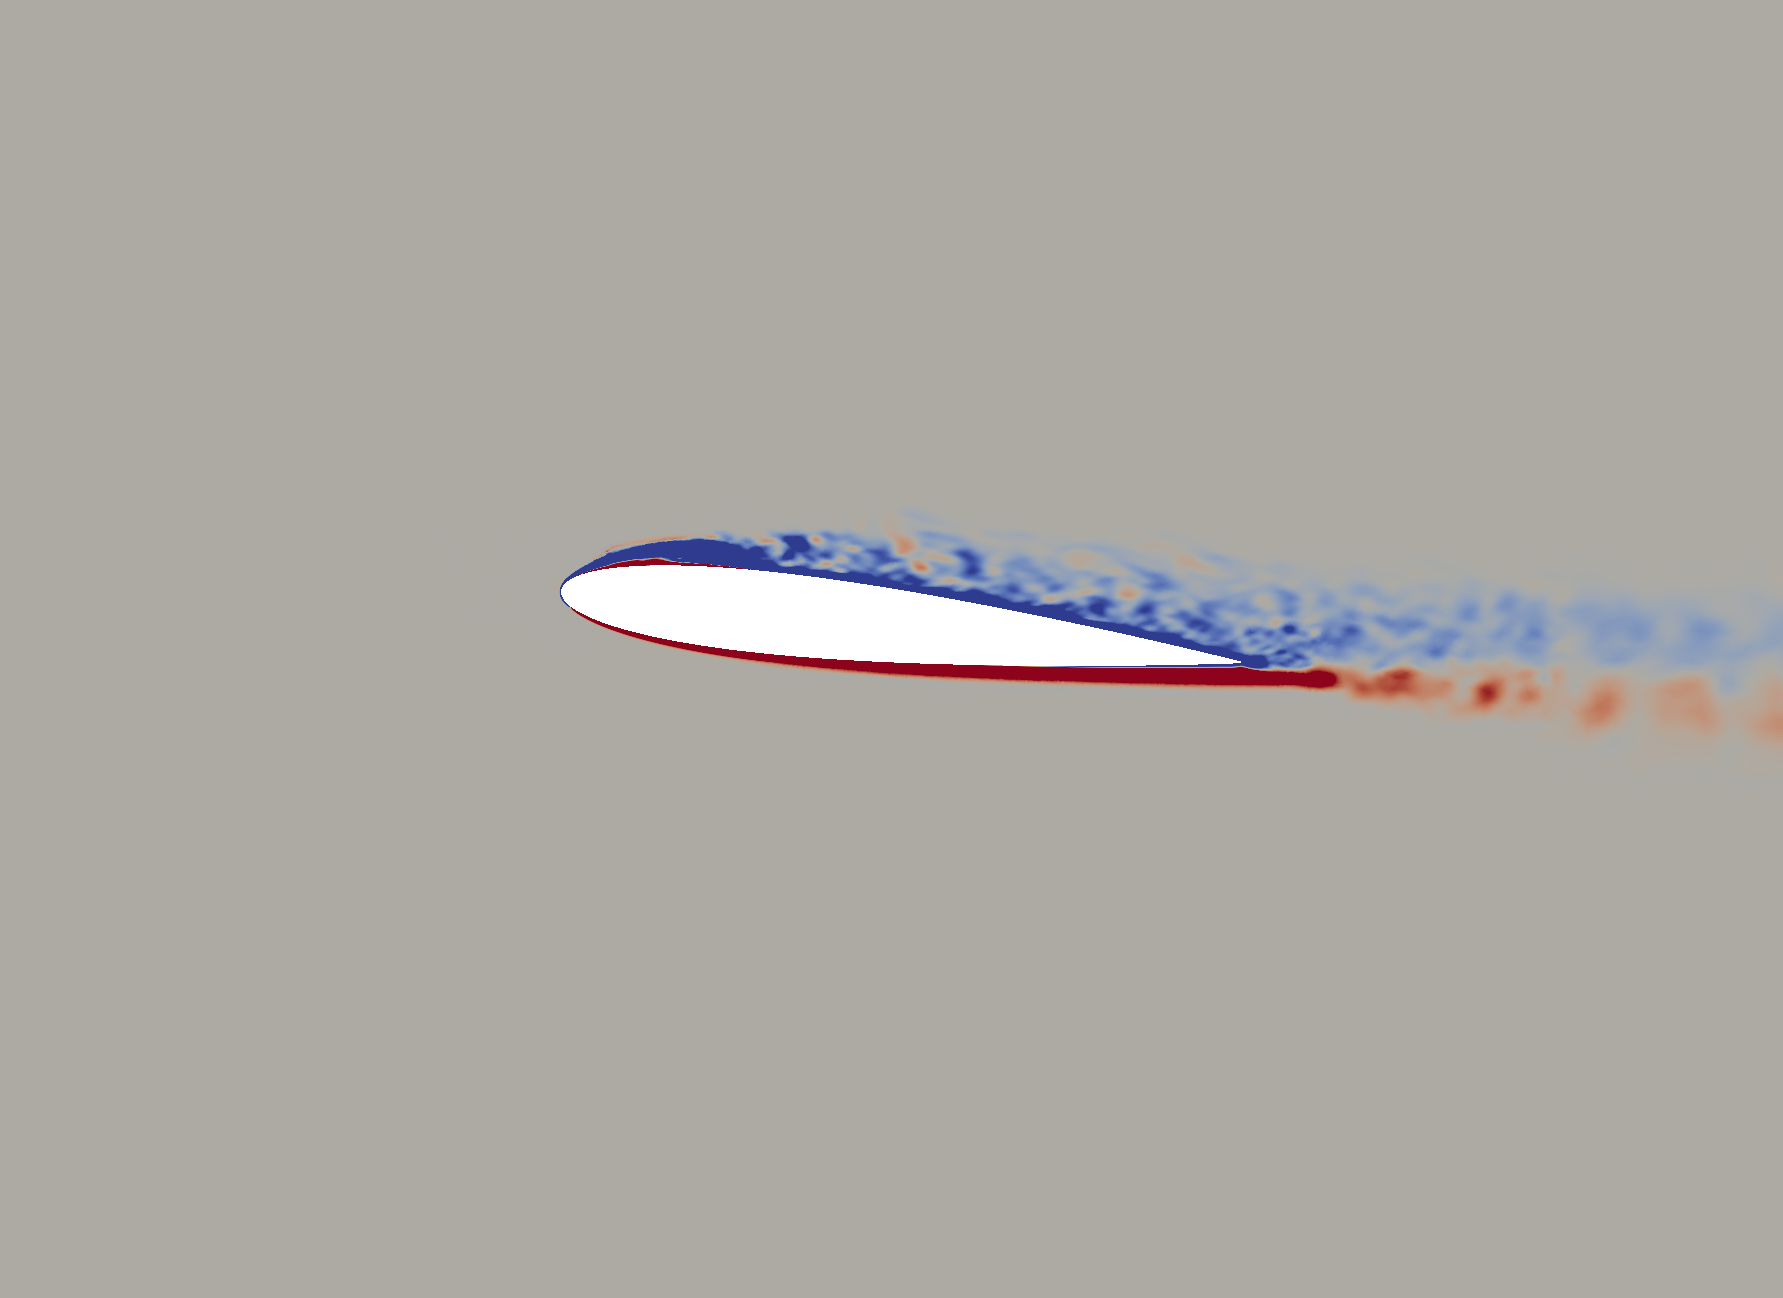
\includegraphics[width=1\textwidth]{figures/Vorticity_plots/Re_40k_1pt2/phase_195.png}
		\caption{$Re= 4e4$, $\psi$ = $195^\circ$, $\tilde{t}=0.542$}
		\label{fig:Re_40k_1pt2_phi195}
	\end{subfigure}
	\begin{subfigure}[b]{0.32\textwidth}
		\centering
		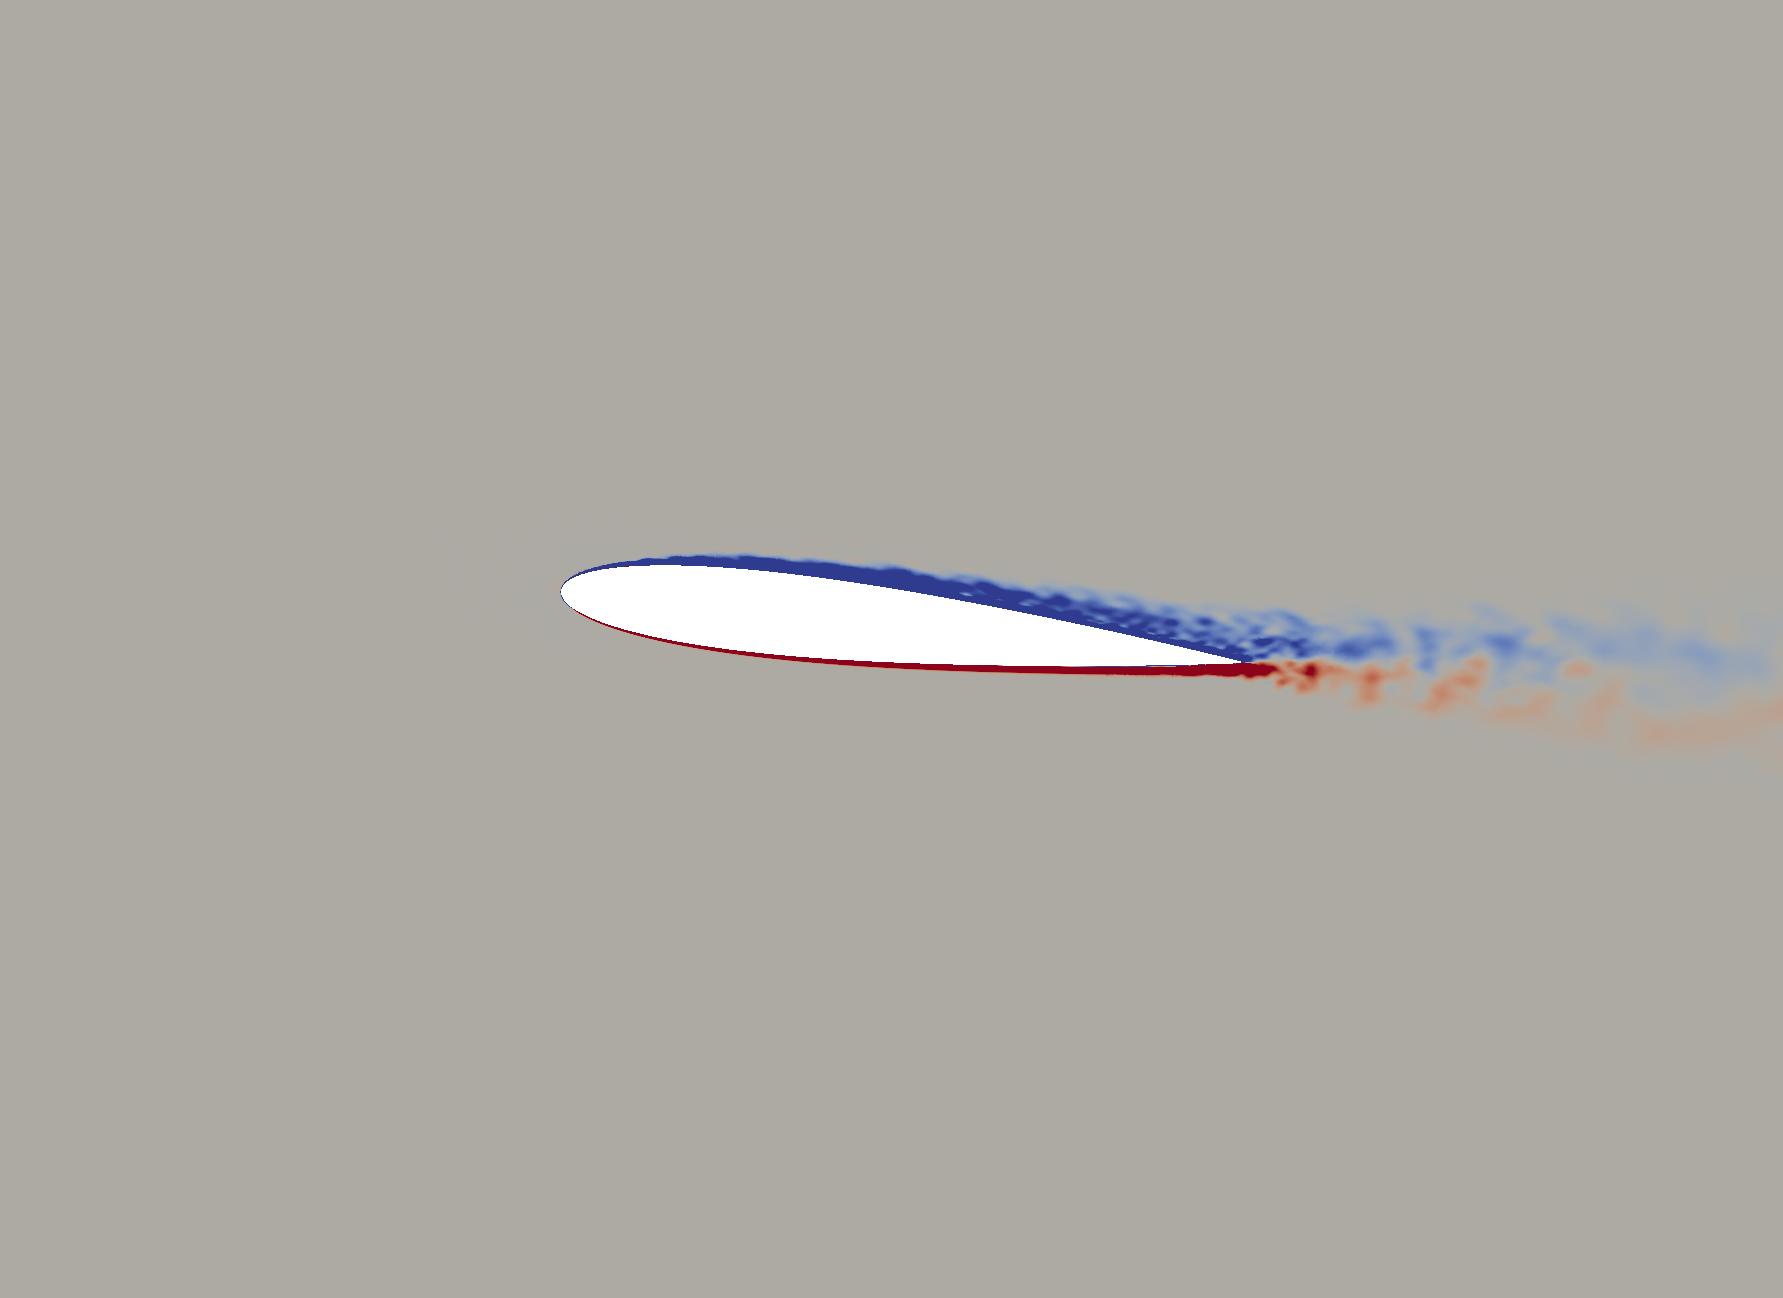
\includegraphics[width=1\textwidth]{figures/Vorticity_plots/Re_200k_1pt2/phase_195.png}
		\caption{$Re=2e5$, $\psi$ = $195^\circ$, $\tilde{t}=0.542$}
		\label{fig:Re_200k_1pt2_phi195}
	\end{subfigure}
	\begin{subfigure}[b]{0.32\textwidth}
		\centering
		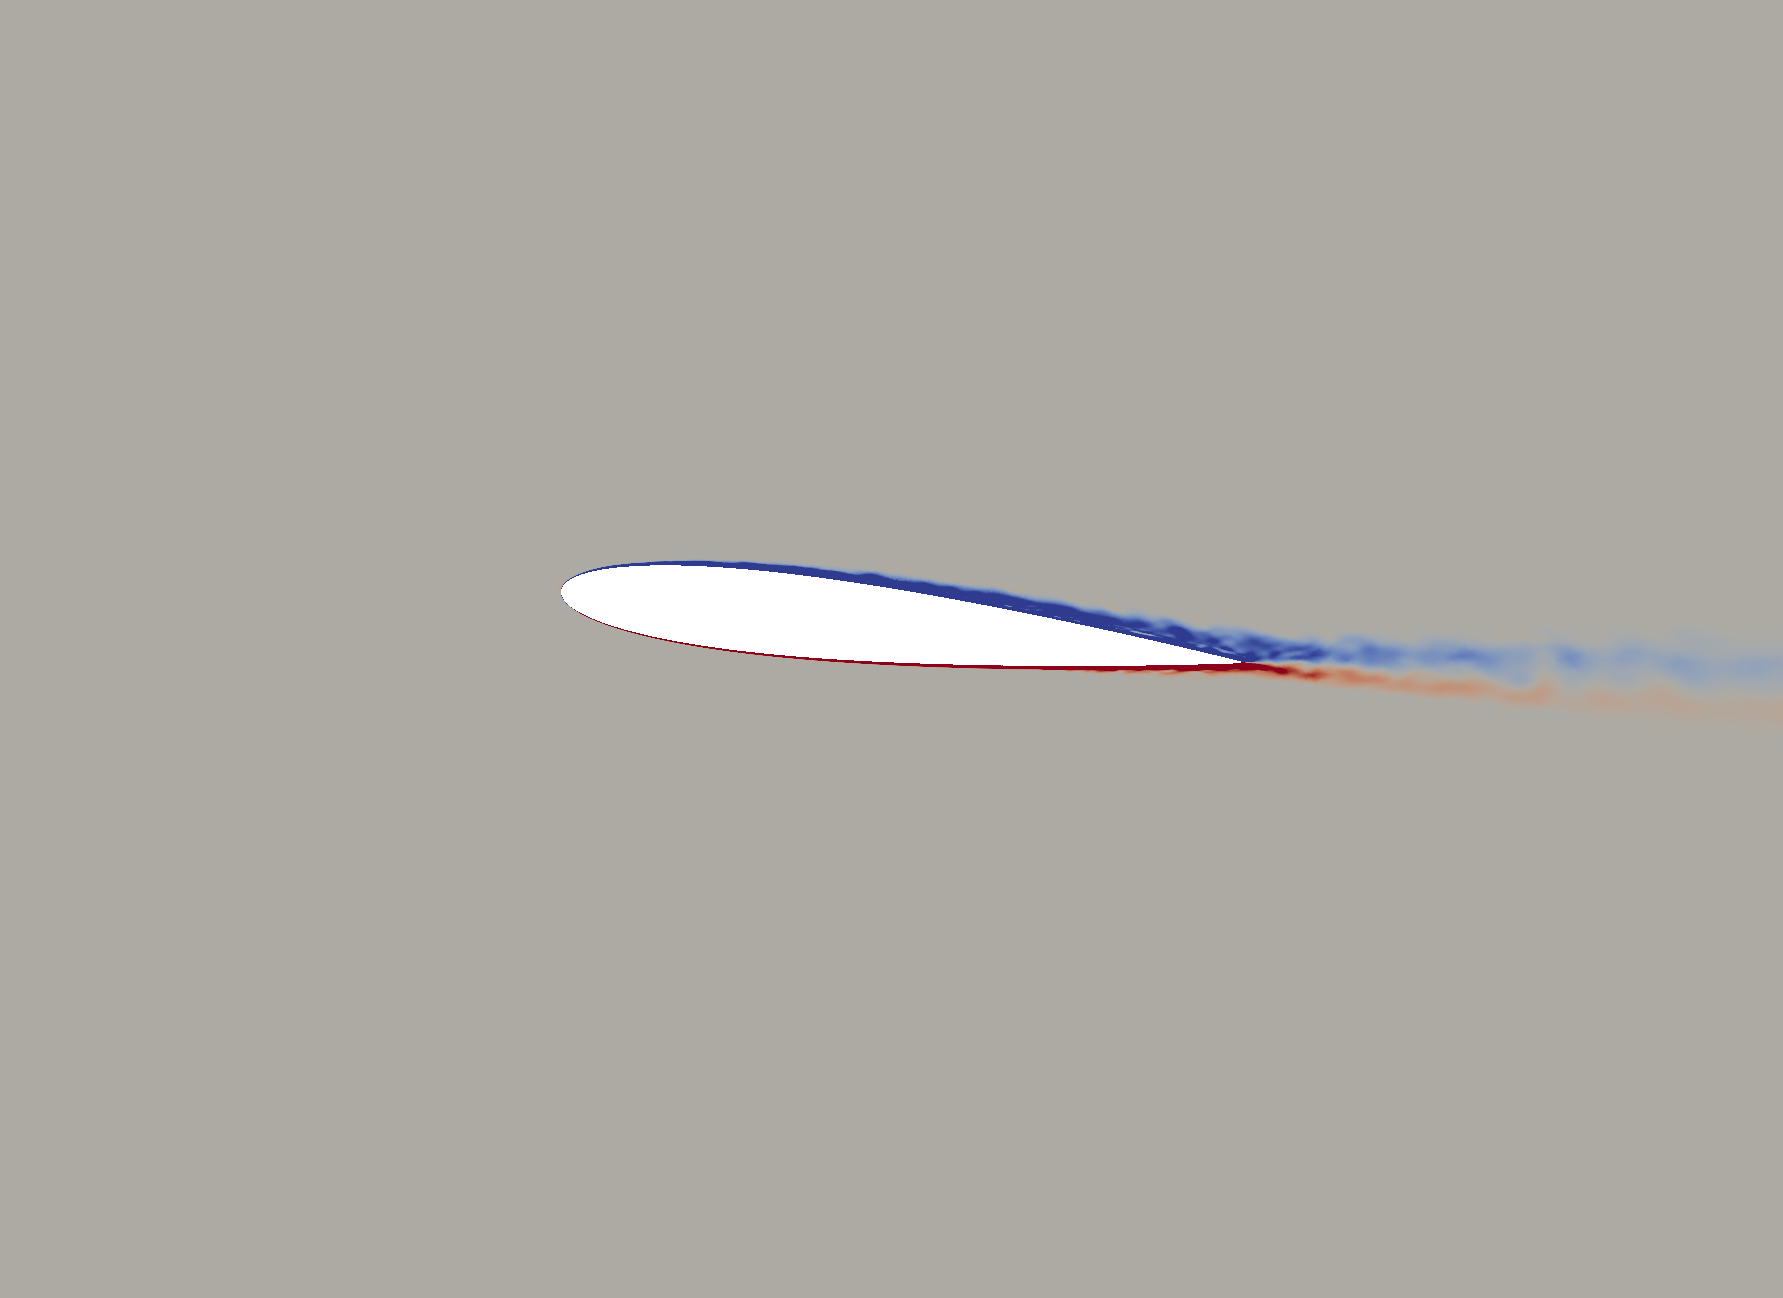
\includegraphics[width=1\textwidth]{figures/Vorticity_plots/Re_1m_1pt2/phase_195.png}
		\caption{$Re= 1e6$, $\psi$ = $195^\circ$, $\tilde{t}=0.542$}
		\label{fig:Re_1m_1pt2_phi195}
	\end{subfigure}
	
	\begin{subfigure}[b]{0.32\textwidth}
		\centering
		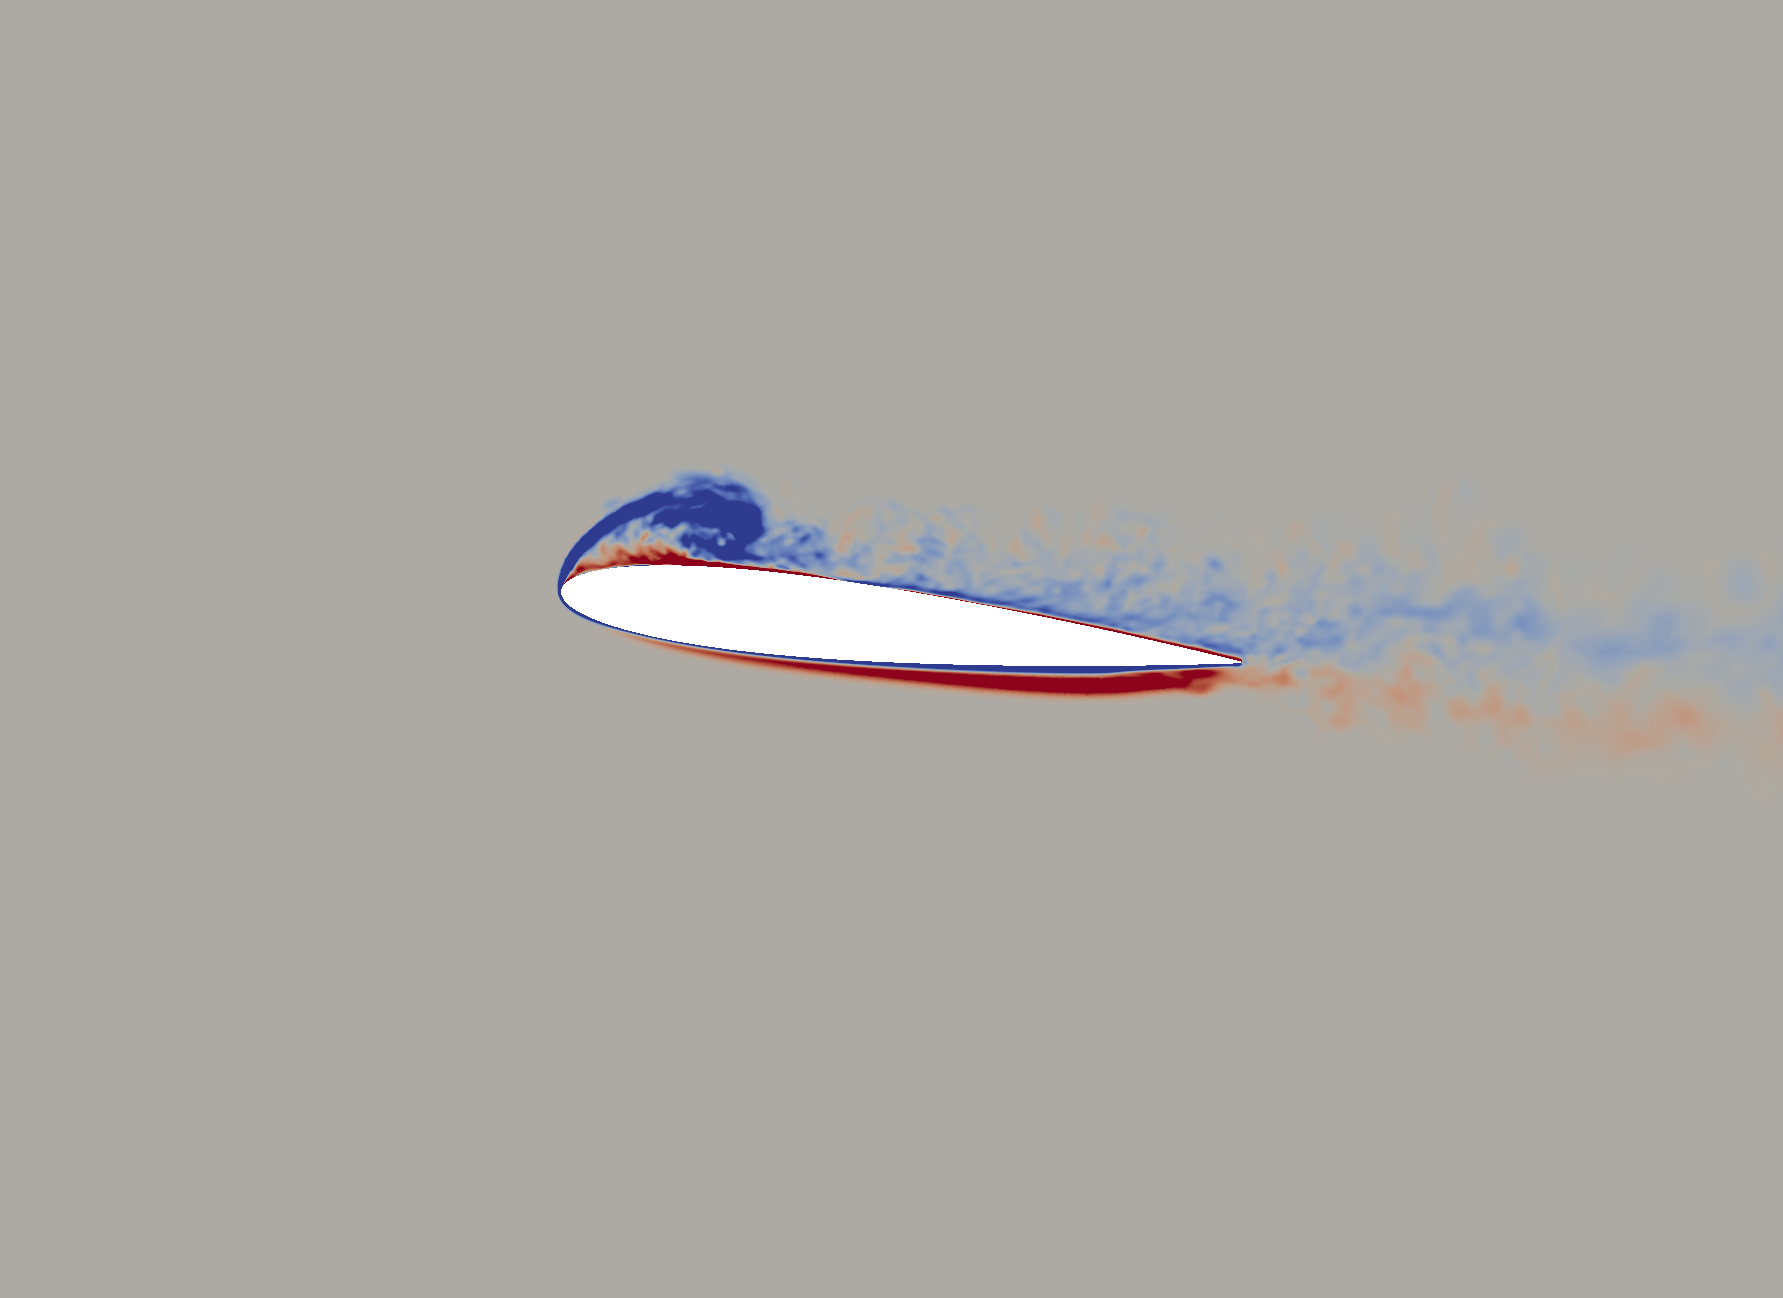
\includegraphics[width=1\textwidth]{figures/Vorticity_plots/Re_40k_1pt2/phase_225.png}
		\caption{$Re=4e4$, $\psi$ = $225^\circ$, $\tilde{t}=0.625$}
		\label{fig:Re_40k_1pt2_phi225}
	\end{subfigure}
	\begin{subfigure}[b]{0.32\textwidth}
		\centering
		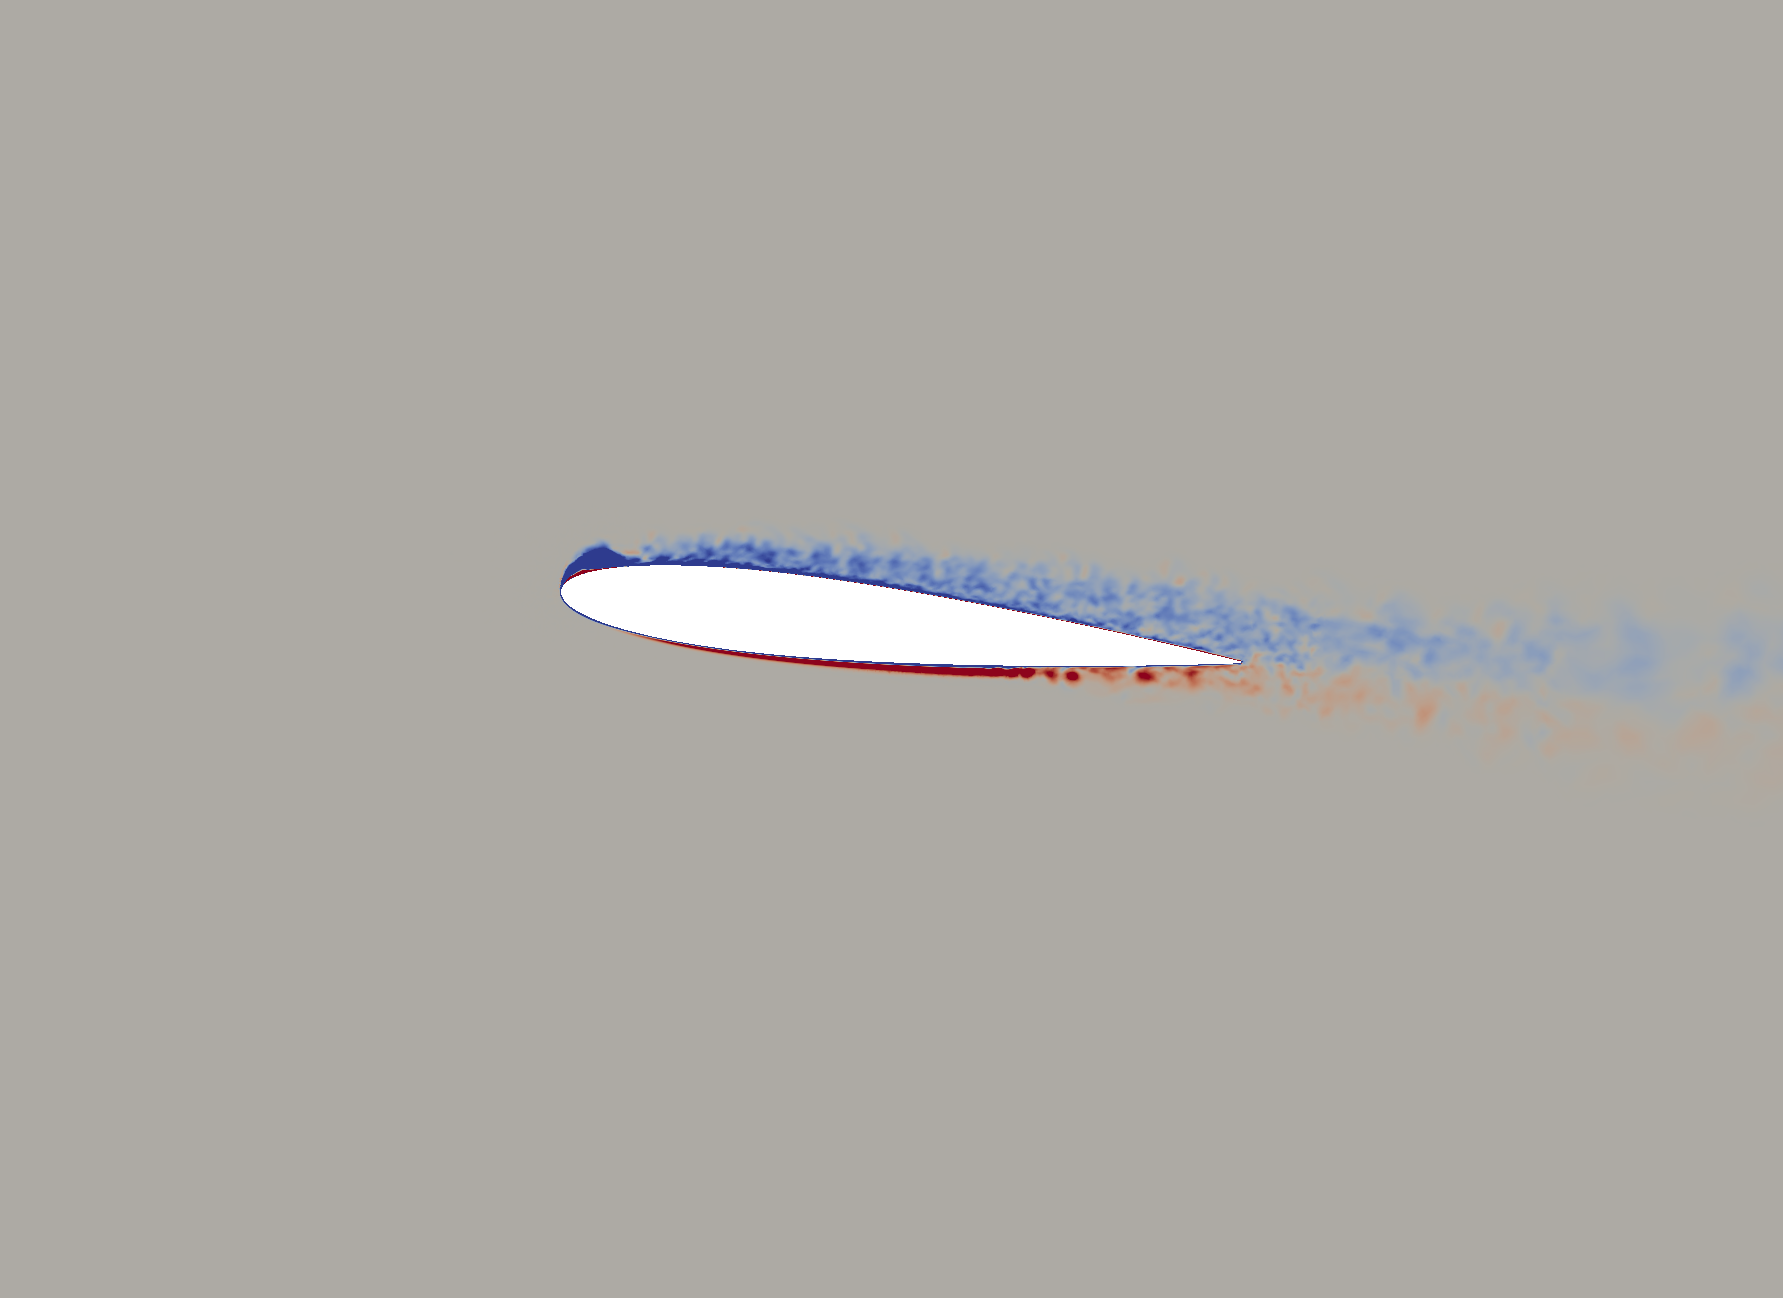
\includegraphics[width=1\textwidth]{figures/Vorticity_plots/Re_200k_1pt2/phase_225.png}
		\caption{$Re=2e5$, $\psi$ = $225^\circ$, $\tilde{t}=0.625$}
		\label{fig:Re_200k_1pt2_phi225}
	\end{subfigure}
	\begin{subfigure}[b]{0.32\textwidth}
		\centering
		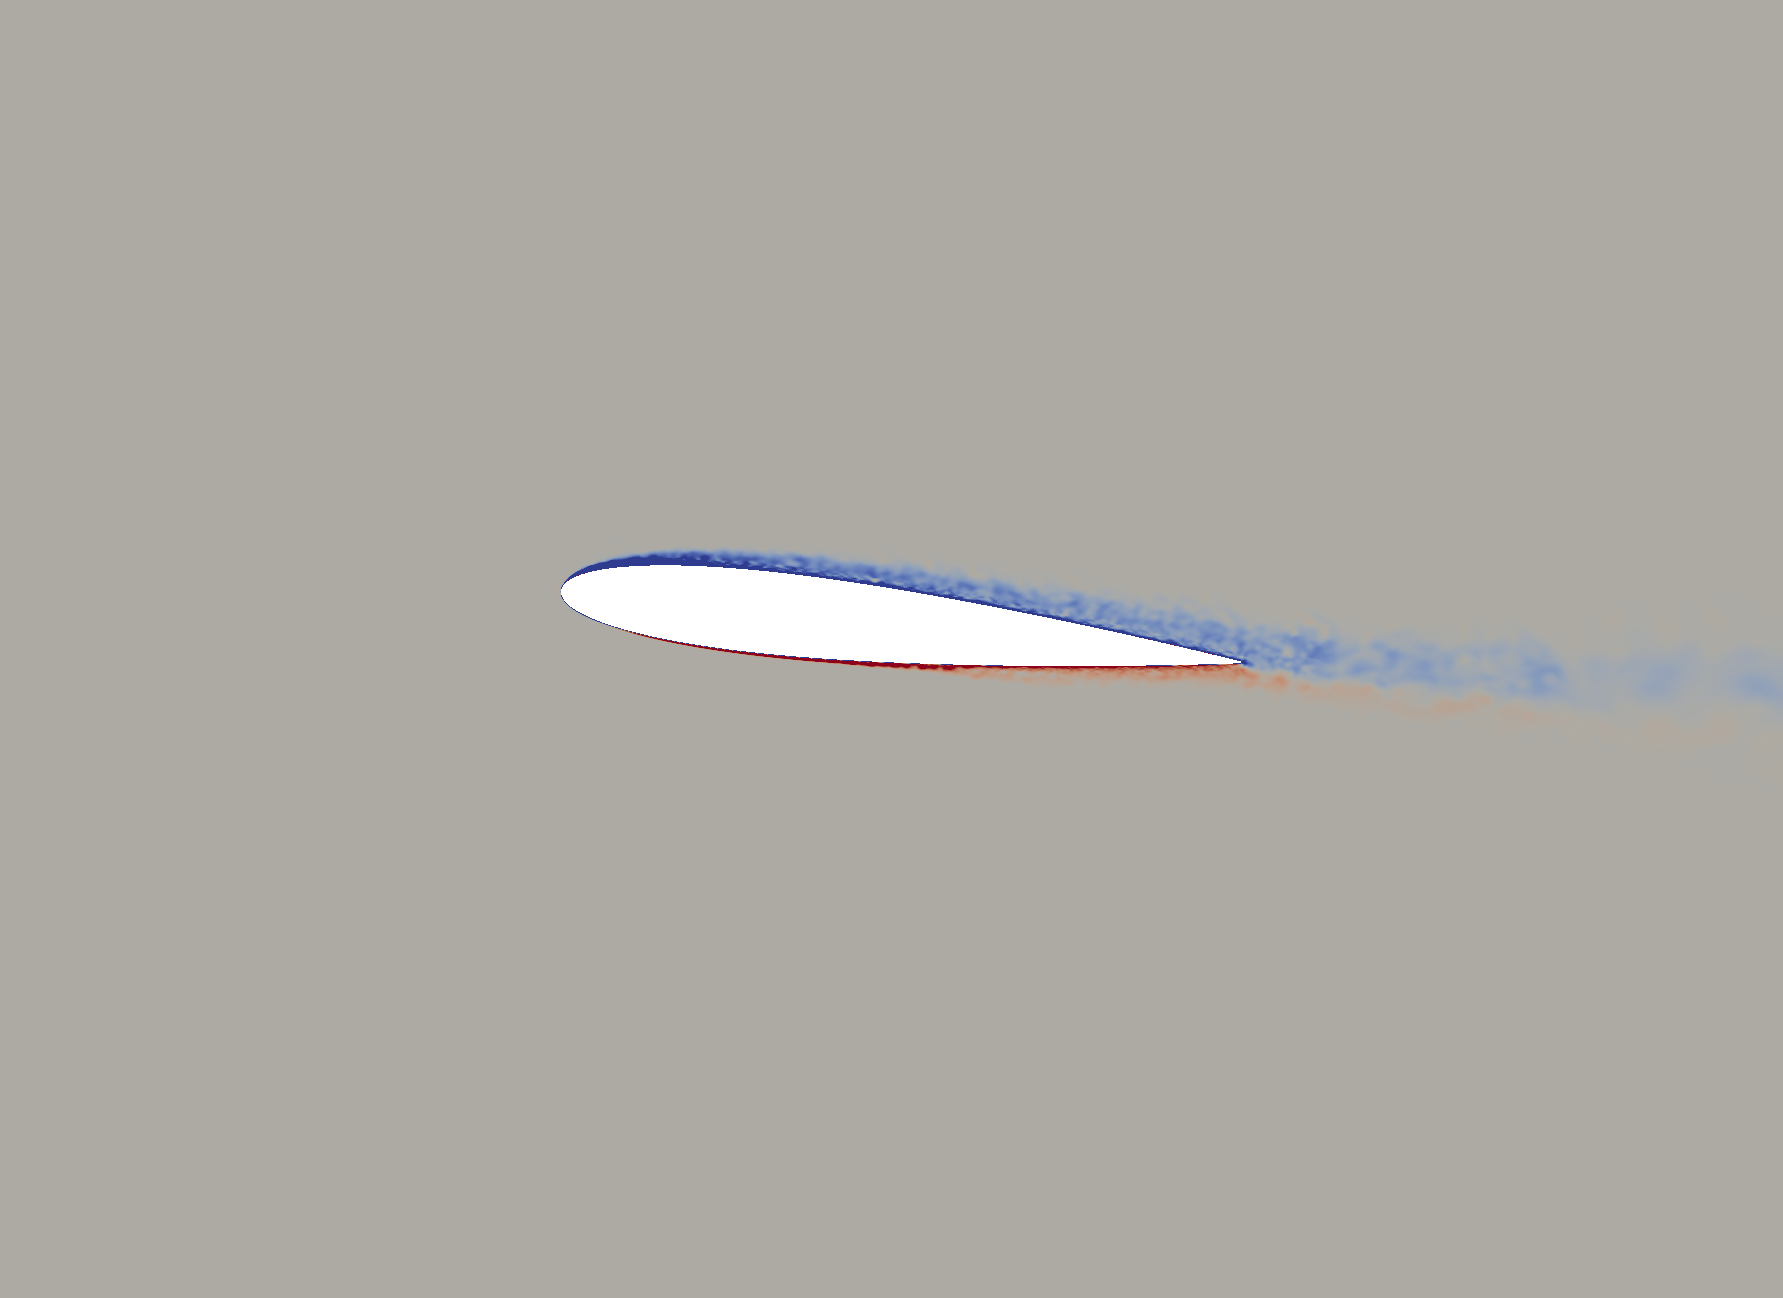
\includegraphics[width=1\textwidth]{figures/Vorticity_plots/Re_1m_1pt2/phase_225.png}
		\caption{$Re=1e6$, $\psi$ = $225^\circ$, $\tilde{t}=0.625$}
		\label{fig:Re_1m_1pt2_phi225}
	\end{subfigure}
	
	\begin{subfigure}[b]{0.32\textwidth}
		\centering
		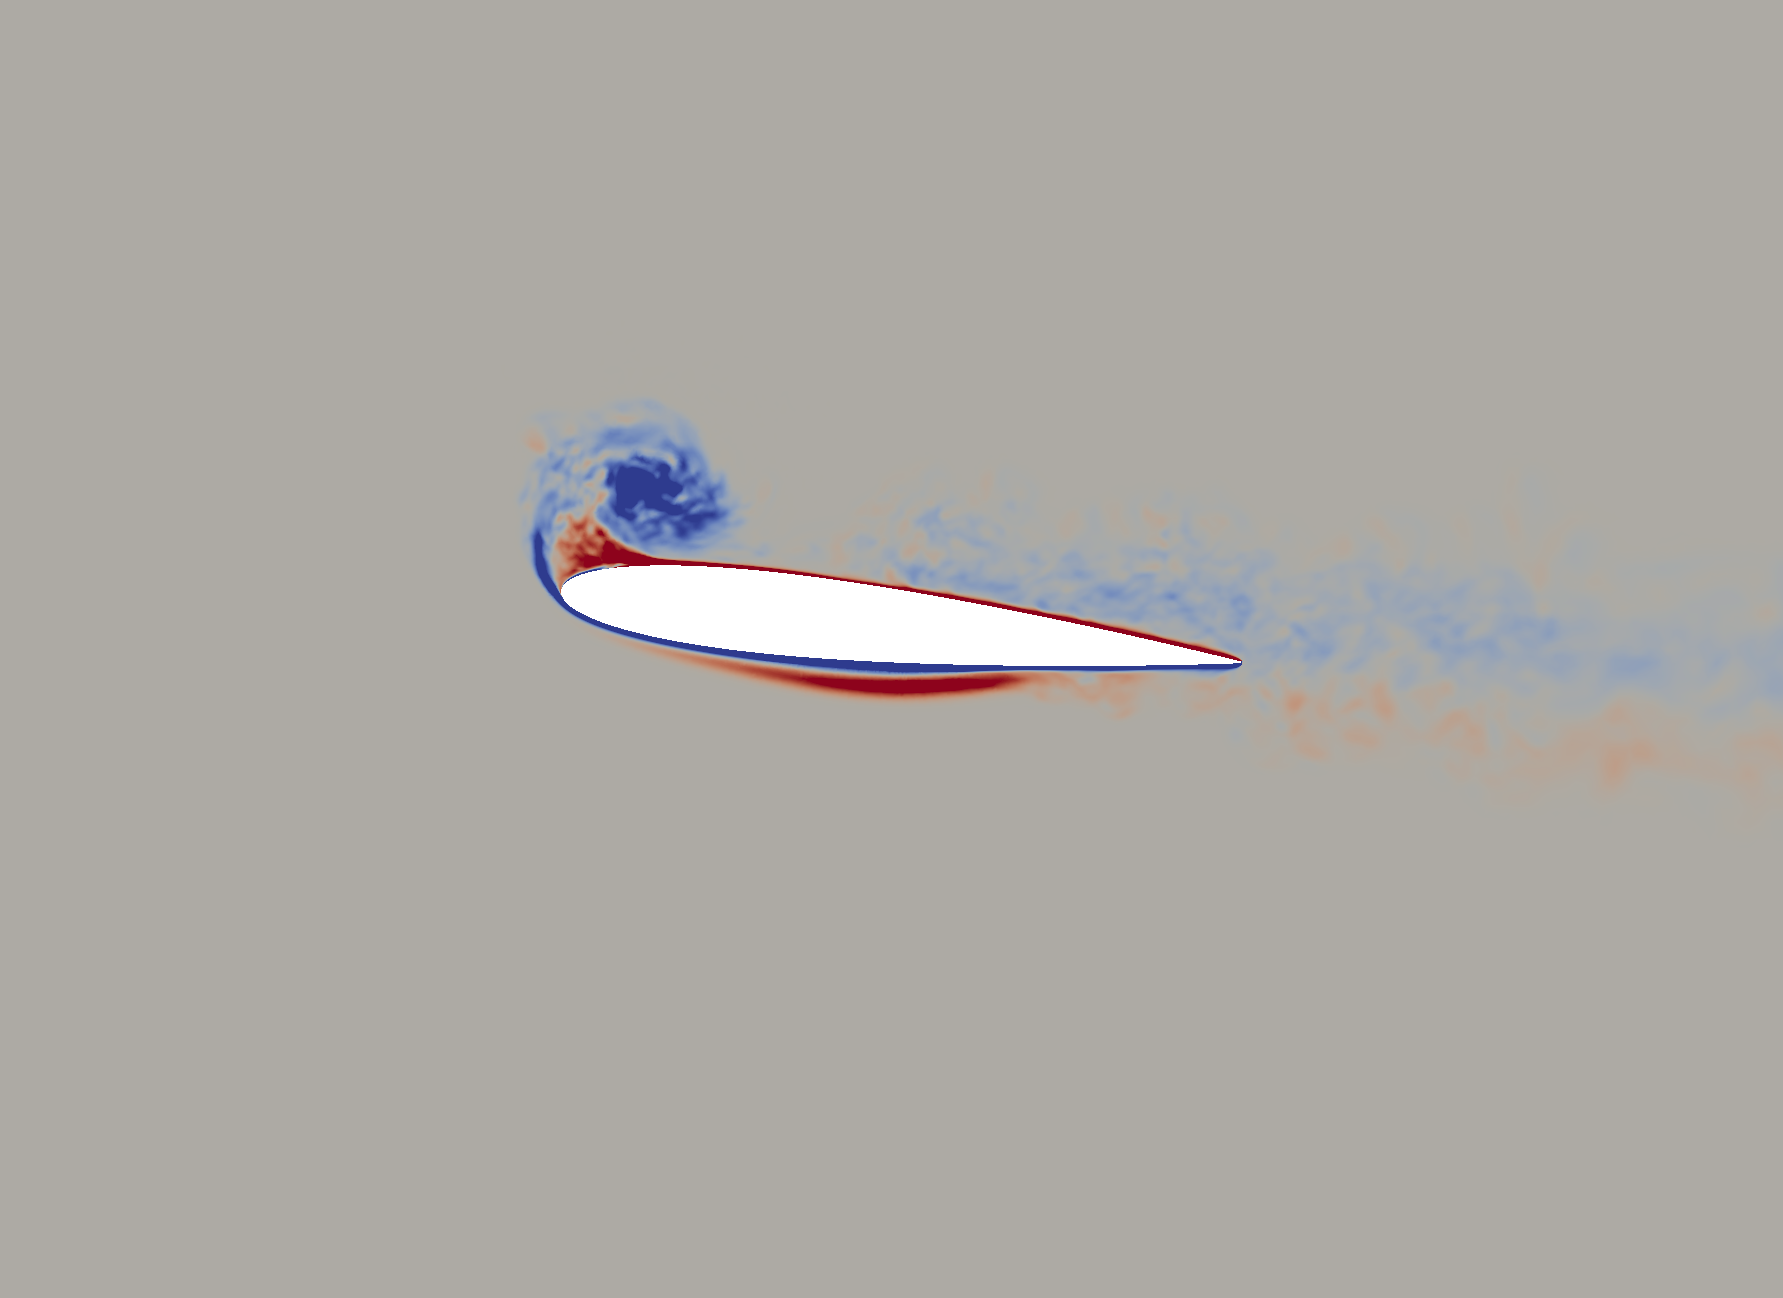
\includegraphics[width=1\textwidth]{figures/Vorticity_plots/Re_40k_1pt2/phase_240.png}
		\caption{$Re=4e4$, $\psi$ = $240^\circ$, $\tilde{t}=0.667$}
		\label{fig:Re_40k_1pt2_phi240}
	\end{subfigure}
	\begin{subfigure}[b]{0.32\textwidth}
		\centering
		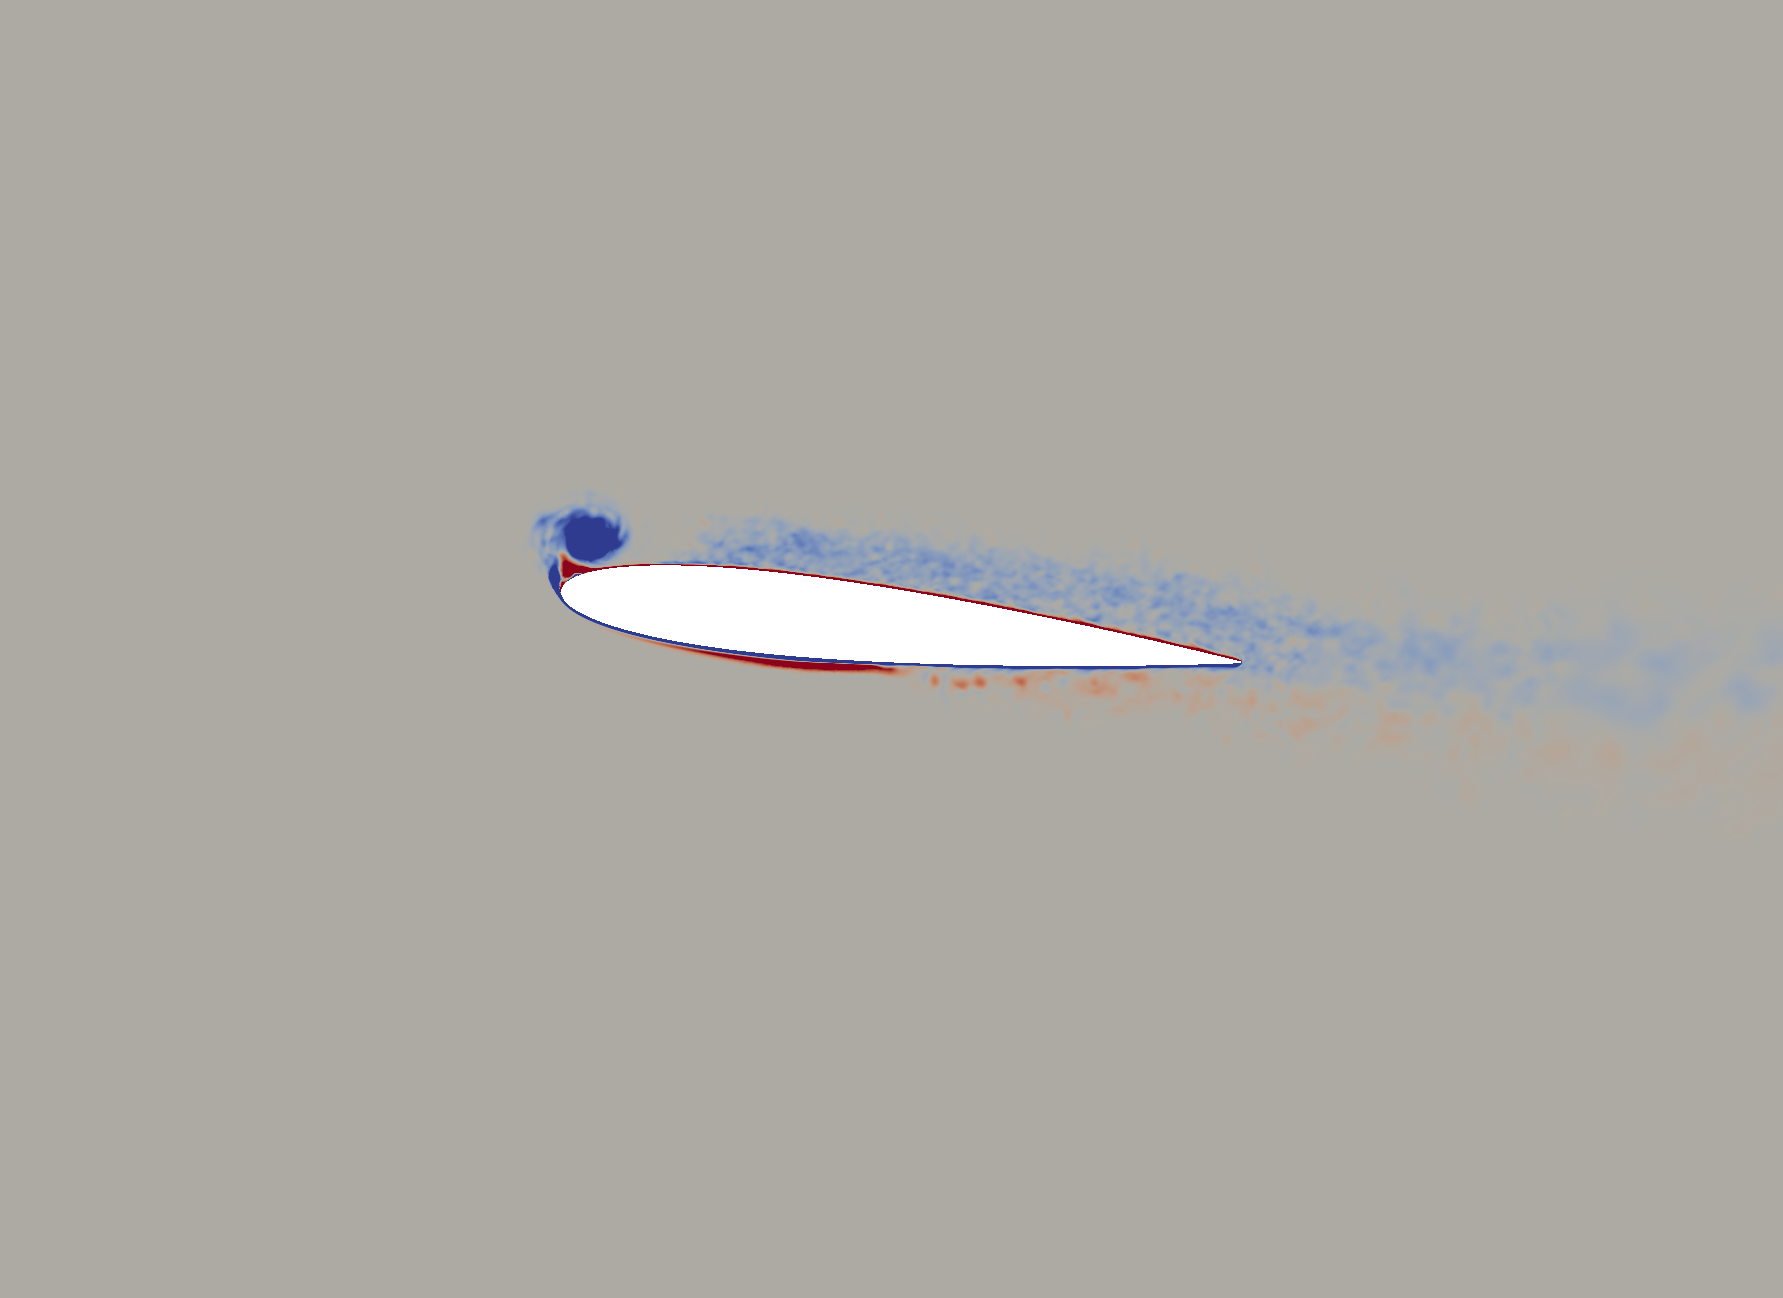
\includegraphics[width=1\textwidth]{figures/Vorticity_plots/Re_200k_1pt2/phase_240.png}
		\caption{$Re=2e5$, $\psi$ = $240^\circ$, $\tilde{t}=0.667$}
		\label{fig:Re_200k_1pt2_phi240}
	\end{subfigure}
	\begin{subfigure}[b]{0.32\textwidth}
		\centering
		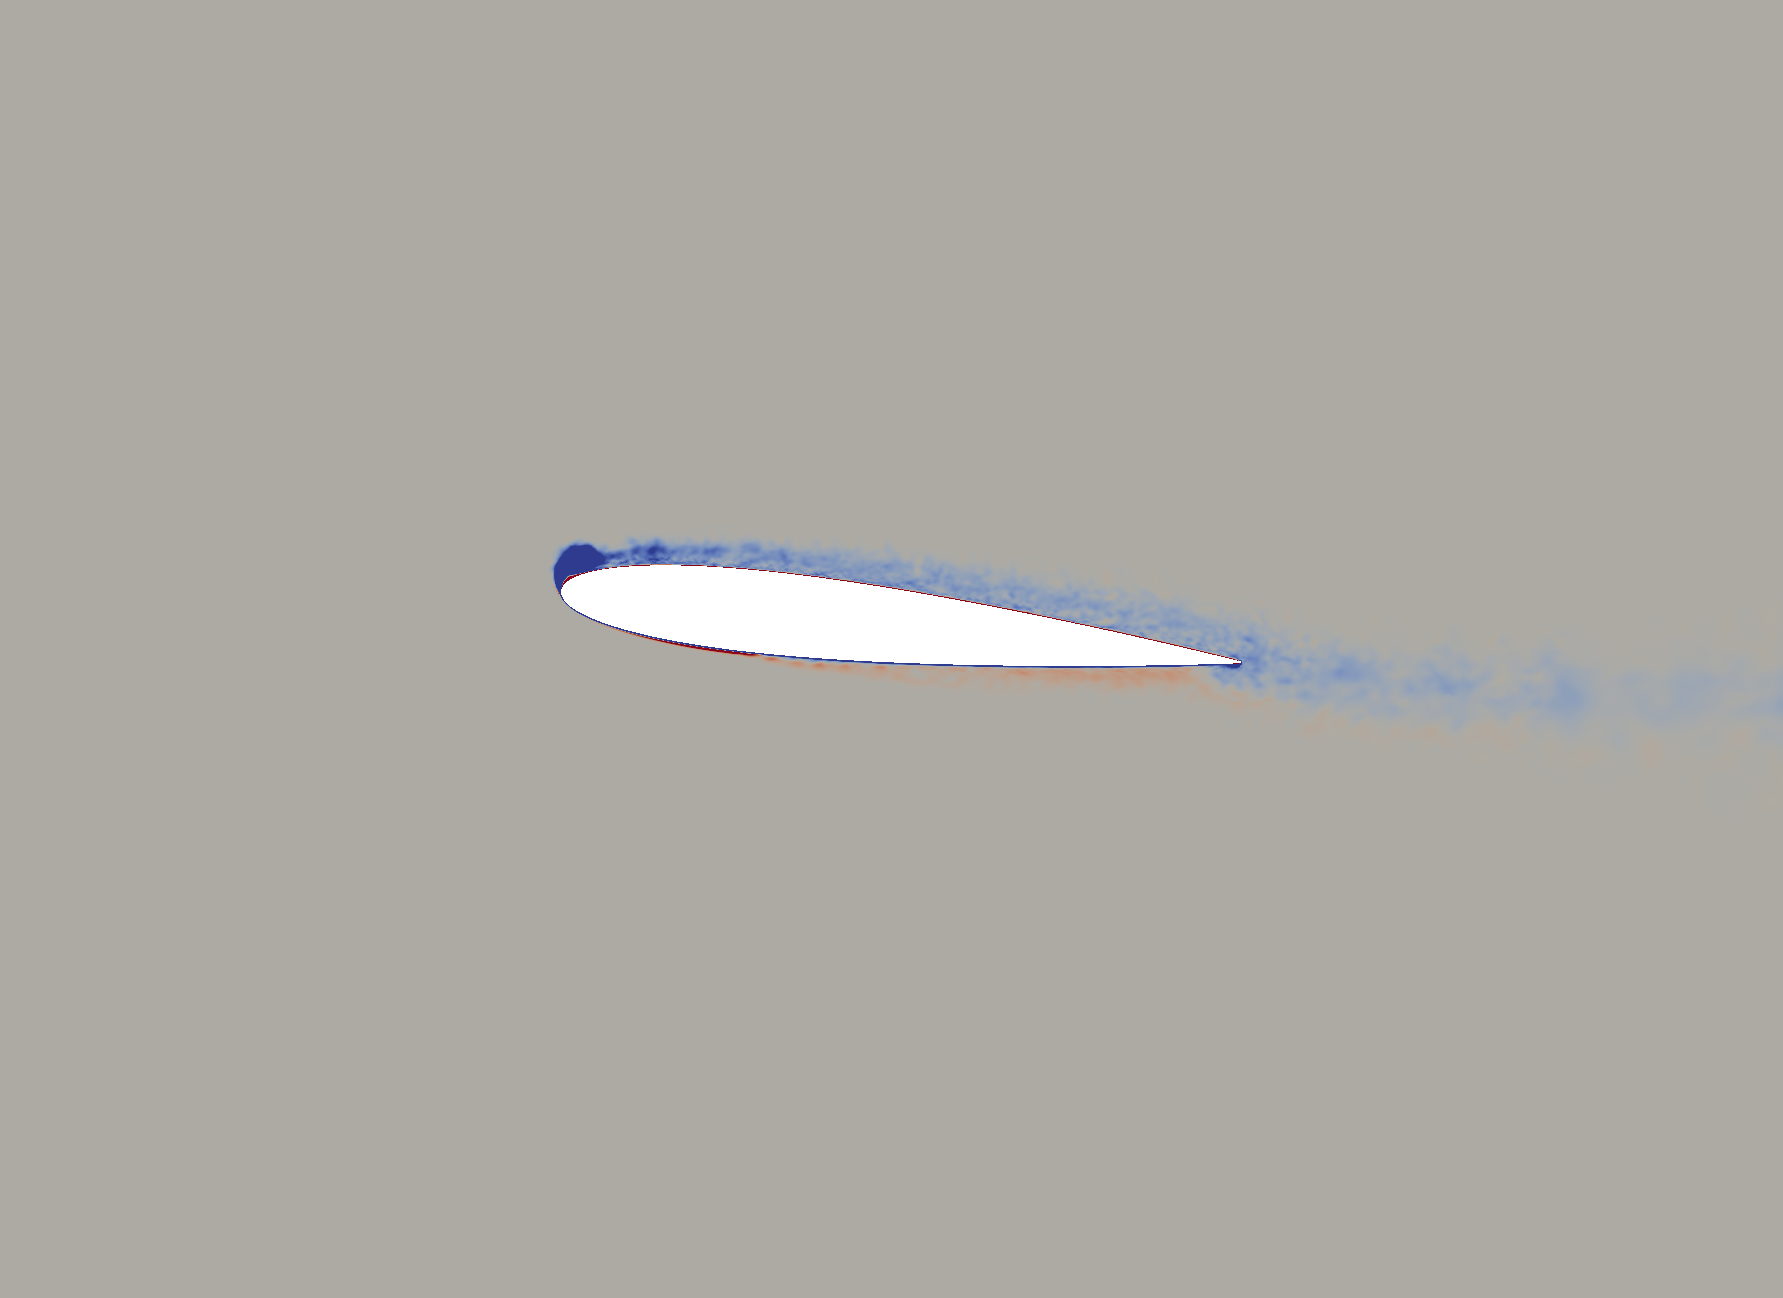
\includegraphics[width=1\textwidth]{figures/Vorticity_plots/Re_1m_1pt2/phase_240.png}
		\caption{$Re=1e6$, $\psi$ = $240^\circ$, $\tilde{t}=0.667$}
		\label{fig:Re_1m_1pt2_phi240}
	\end{subfigure}
	
	\begin{subfigure}[b]{0.32\textwidth}
		\centering
		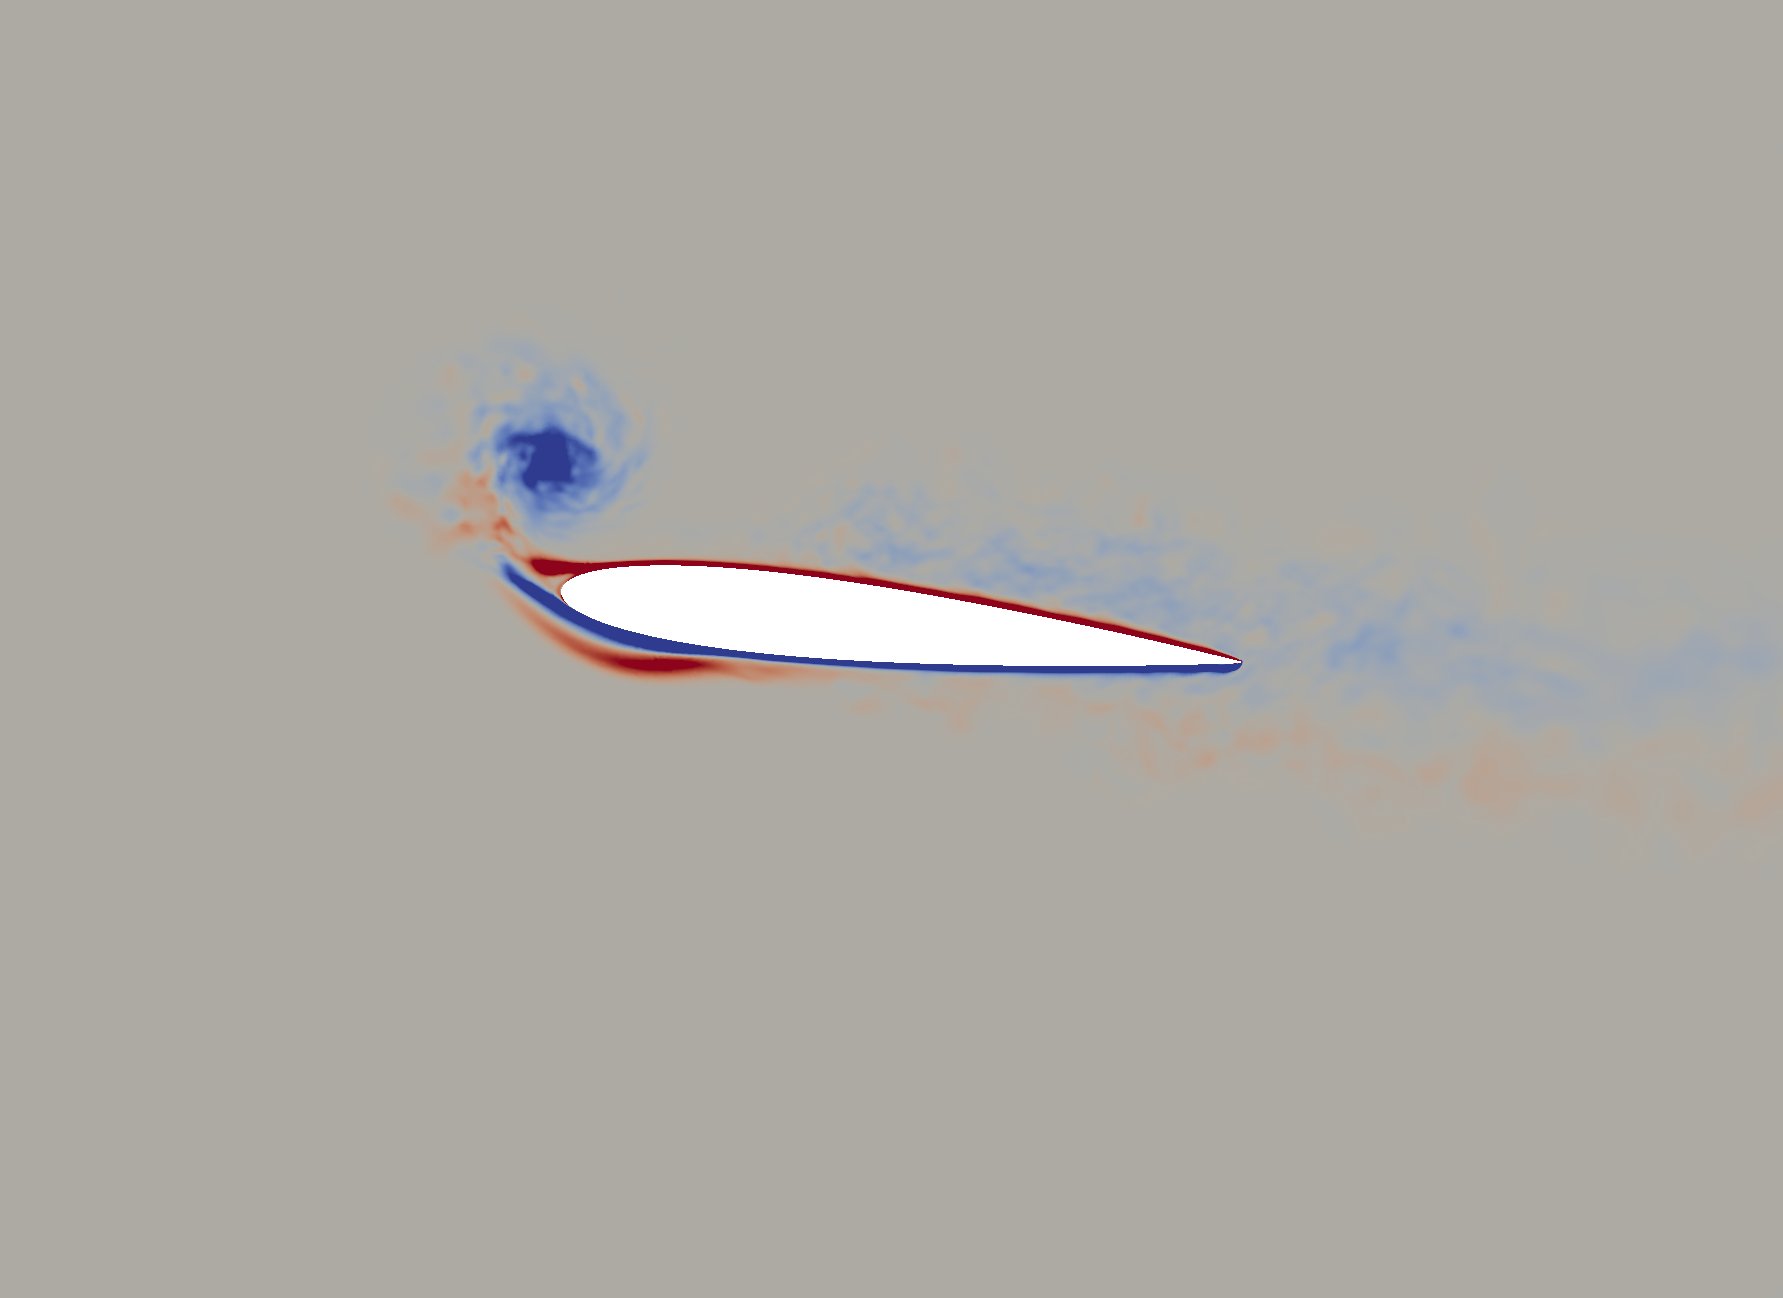
\includegraphics[width=1\textwidth]{figures/Vorticity_plots/Re_40k_1pt2/phase_255.png}
		\caption{$Re=4e4$, $\psi$ = $255^\circ$, $\tilde{t}=0.708$}
		\label{fig:Re_40k_1pt2_phi255}
	\end{subfigure}
	\begin{subfigure}[b]{0.32\textwidth}
		\centering
		\includegraphics[width=1\textwidth]{figures/Vorticity_plots/Re_200k_1pt2/phase_255.png}
		\caption{$Re=2e5$, $\psi$ = $255^\circ$, $\tilde{t}=0.708$}
		\label{fig:Re_200k_1pt2_phi255}
	\end{subfigure}
	\begin{subfigure}[b]{0.32\textwidth}
		\centering
		\includegraphics[width=1\textwidth]{figures/Vorticity_plots/Re_1m_1pt2/phase_255.png}
		\caption{$Re=1e6$, $\psi$ = $255^\circ$, $\tilde{t}=0.708$}
		\label{fig:Re_1m_1pt2_phi255}
	\end{subfigure}
	
	\caption{Spanwise vorticity at 8 different phases for $Re$=40,000 (left column), 200,000 (middle column) and 1,000,000 (right column) at $\mu_{sect}$ = 1.2}
%	\label{fig:vortScreen_1pt2}
\end{figure}


\begin{figure}[H]\ContinuedFloat
	\centering
	\begin{subfigure}[b]{0.32\textwidth}
		\centering
		\includegraphics[width=1\textwidth]{figures/Vorticity_plots/Re_40k_1pt2/phase_270.png}
		\caption{$Re=4e4$, $\psi$ = $270^\circ$, $\tilde{t}=0.750$}
		\label{fig:Re_40k_1pt2_phi270}
	\end{subfigure}
	\begin{subfigure}[b]{0.32\textwidth}
		\centering
		\includegraphics[width=1\textwidth]{figures/Vorticity_plots/Re_200k_1pt2/phase_270.png}
		\caption{$Re=2e5$, $\psi$ = $270^\circ$, $\tilde{t}=0.750$}
		\label{fig:Re_200k_1pt2_phi270}
	\end{subfigure}
	\begin{subfigure}[b]{0.32\textwidth}
		\centering
		\includegraphics[width=1\textwidth]{figures/Vorticity_plots/Re_1m_1pt2/phase_270.png}
		\caption{$Re=1e6$, $\psi$ = $270^\circ$, $\tilde{t}=0.750$}
		\label{fig:Re_1m_1pt2_phi270}
	\end{subfigure}
	
	\begin{subfigure}[b]{0.32\textwidth}
		\centering
		\includegraphics[width=1\textwidth]{figures/Vorticity_plots/Re_40k_1pt2/phase_315.png}
		\caption{$Re=4e4$, $\psi$ = $315^\circ$, $\tilde{t}=0.875$}
		\label{fig:Re_40k_1pt2_phi315}
	\end{subfigure}
	\begin{subfigure}[b]{0.32\textwidth}
		\centering
		\includegraphics[width=1\textwidth]{figures/Vorticity_plots/Re_200k_1pt2/phase_315.png}
		\caption{$Re=2e5$, $\psi$ = $315^\circ$, $\tilde{t}=0.875$}
		\label{fig:Re_200k_1pt2_phi315}
	\end{subfigure}
	\begin{subfigure}[b]{0.32\textwidth}
		\centering
		\includegraphics[width=1\textwidth]{figures/Vorticity_plots/Re_1m_1pt2/phase_315.png}
		\caption{$Re=1e6$, $\psi$ = $315^\circ$, $\tilde{t}=0.875$}
		\label{fig:Re_1m_1pt2_phi315}
	\end{subfigure}
	
	\begin{subfigure}[b]{0.32\textwidth}
		\centering
		\includegraphics[width=1\textwidth]{figures/Vorticity_plots/Re_40k_1pt2/phase_330.png}
		\caption{$Re=4e4$, $\psi$ = $330^\circ$, $\tilde{t}=0.917$}
		\label{fig:Re_40k_1pt2_phi330}
	\end{subfigure}
	\begin{subfigure}[b]{0.32\textwidth}
		\centering
		\includegraphics[width=1\textwidth]{figures/Vorticity_plots/Re_200k_1pt2/phase_330.png}
		\caption{$Re=2e5$, $\psi$ = $330^\circ$, $\tilde{t}=0.917$}
		\label{fig:Re_200k_1pt2_phi330}
	\end{subfigure}
	\begin{subfigure}[b]{0.32\textwidth}
		\centering
		\includegraphics[width=1\textwidth]{figures/Vorticity_plots/Re_1m_1pt2/phase_330.png}
		\caption{$Re=1e6$,$\psi$ = $330^\circ$, $\tilde{t}=0.917$}
		\label{fig:Re_1m_1pt2_phi330}
	\end{subfigure}	
	\begin{subfigure}[b]{0.32\textwidth}
		\centering
		\includegraphics[width=1\textwidth]{figures/Vorticity_plots/Re_40k_1pt2/phase_345.png}
		\caption{$Re=4e4$, $\psi$ = $345^\circ$, $\tilde{t}=0.958$}
		\label{fig:Re_40k_1pt2_phi345}
	\end{subfigure}
	\begin{subfigure}[b]{0.32\textwidth}
		\centering
		\includegraphics[width=1\textwidth]{figures/Vorticity_plots/Re_200k_1pt2/phase_345.png}
		\caption{$Re=2e5$, $\psi$ = $345^\circ$, $\tilde{t}=0.958$}
		\label{fig:Re_200k_1pt2_phi345}
	\end{subfigure}
	\begin{subfigure}[b]{0.32\textwidth}
		\centering
		\includegraphics[width=1\textwidth]{figures/Vorticity_plots/Re_1m_1pt2/phase_345.png}
		\caption{$Re=1e6$,$\psi$ = $345^\circ$, $\tilde{t}=0.958$}
		\label{fig:Re_1m_1pt2_phi345}
	\end{subfigure}
	
	\caption{Spanwise vorticity at 8 different phases for $Re$=40,000 (left column), 200,000 (middle column) and 1,000,000 (right column) at $\mu_{sect}$ = 1.2}
	\label{fig:vortScreen_1pt2}
\end{figure}

\subsection{LEV Evolution}
\label{sec:LEV}

%TODO: Use pics from presentation

LEV detection and tracking is performed using the procedure developed in this work, see Section \ref{sec:LEV_detect_track}. LEV position with respect to the leading edge of the airfoil is presented in Figure~\ref{fig:LEV_location_LE_airfoil}.
In the $\mu_{sect}=1.0$ case, the initial position of the LEV (i.e., position at formation) gets closer to the leading edge as the Reynolds number is increased.
Further, LEV remains closest to the airfoil over the cycle for the highest Reynolds number of $Re$=1,000,000 (i.e., note the vertical position of the LEV).
On the other hand, LEV initially moves to the left (towards the geometric leading edge) from its initial position for the lowest Reynolds number of $Re$=40,000.
In the $\mu_{sect}=1.2$ case also, similar trends are observed.
However, at the higher advance ratio the LEV initially moves to the left past the geometric leading edge for each Reynolds number.
This is expected since the relative flow velocity becomes negative (or a reversed flow condition is obtained) at $\mu_{sect}=1.2$.

Figure \ref{fig:LEV_size} presents the size or core radius ($r_c$) of the LEV for all six cases.
We note that in simulations the data was recorded at every $\Delta \psi = 15^\circ$ starting at $\psi$=$15^\circ$.
For each case the LEV is formed at about $\tilde{t}=0.6$ or later.
The LEV size is higher for the lowest Reynolds number of $Re$=40,000 for both advance ratios of $\mu_{sect}$=1.0 and 1.2.
This is expected since the boundary layer is thicker for $Re$=40,000 and the resulting separated shear layer rolls up into a larger LEV.
The LEV size is very similar for the other two higher Reynolds numbers at $\mu_{sect}$=1.0 and 1.2.
In the $\mu_{sect}$=1.0 case, the LEV increases in size till about $\tilde{t}=0.75$ to 0.8 and subsequently seem to plateau or increase in size relatively slowly.
Towards the end of the cycle, the LEV size is predicted to be about 8\% of the chord for $Re$=40,000 at $\mu_{sect}$=1.0, and about 6\% for $Re$=200,000 and 1,000,000 at $\mu_{sect}$=1.0.
In the $\mu_{sect}$=1.2 case, the LEV increases in size throughout the cycle and towards the end of the cycle reaches about a similar size as the $\mu_{sect}$=1.0 case for each Reynolds number. Note that such a quantification of LEV evolution, based on feature/vortex detection and tracking procedure, is also useful for feature-based adaptivity, which is discussed in Section \ref{sec:feature_based_strat}.

\begin{figure}[H]
	\begin{subfigure}{0.5\textwidth}
		\includegraphics[width=1\textwidth]{figures/LEV_size_lambda_1pt0.png}
		\caption{$\mu_{sect} = 1.0$}
		\label{fig:LEV_size_lambda_1p0}
	\end{subfigure}
 	\begin{subfigure}{0.5\textwidth}
	\includegraphics[width=1\textwidth]{figures/LEV_size_lambda_1pt2.png}
	\caption{$\mu_{sect} = 1.2$}
	\label{fig:LEV_size_lambda_1p2}
	\end{subfigure}
 	\caption{LEV evolution: LEV size for $Re$=40,000 (green line with open triangles), 200,000 (red line with closed circles) and 1,000,000 (blue line with open circles) at $\mu_{sect}$=1.0 and 1.2}
 	\label{fig:LEV_size}
\end{figure}




%TODO: indicate we consider Re=40k and 200k for adaptive LES and carefully investigate mesh convergence. this was done for cost savings since LEV exhibits a similar behavior for Re=200k and Re=1m cases.

\begin{figure}[H]
	\begin{subfigure}{0.5\textwidth}
		\includegraphics[width=1\textwidth]{figures/LEV_location_lambda_1pt0}
		\caption{$\mu_{sect} = 1.0$}
		\label{fig:LEV_location_lambda_1p0}
	\end{subfigure}
	\begin{subfigure}{0.5\textwidth}
		\includegraphics[width=1\textwidth]{figures/LEV_location_lambda_1pt2}
		\caption{$\mu_{sect} = 1.2$}
		\label{fig:LEV_location_lambda_1p2}
	\end{subfigure}
 	\caption{LEV evolution: LEV position (with respect to the leading edge of the airfoil) for $Re$=40,000 (green line with open triangles), 200,000 (red line with closed circles) and 1,000,000 (blue line with open circles) at $\mu_{sect}$=1.0 and 1.2}
	\label{fig:LEV_location_LE_airfoil}
\end{figure}

In Figure \ref{fig:LEV_delta_x}, the horizontal displacement of the LEV with respect to the ground is presented.
The displacement is taken about the initial position when the LEV is formed, i.e., the displacement is zero at the initial position.
Again, as the Reynolds number increases the LEV is formed later in the cycle (for a given advance ratio) while as the advance ratio increases it is formed earlier in the cycle (for a given Reynolds number).

An important aspect to note in Figure \ref{fig:LEV_delta_x} is that the horizontal displacement of the LEV follows a straight line for each case and is parallel among all cases.
The slope of the horizontal displacement in each case is remarkably close to the free-stream velocity, i.e., the LEV is advected in the horizontal direction at the free-stream velocity.

\begin{figure}[H]
	\begin{subfigure}{0.5\textwidth}
		\includegraphics[width=1\textwidth]{figures/LEV_deltax_lambda_1pt0.png}
		\caption{$\mu_{sect} = 1.0$}
		\label{fig:LEV_deltax_lambda_1p0}
	\end{subfigure}
	\begin{subfigure}{0.5\textwidth}
		\includegraphics[width=1\textwidth]{figures/LEV_deltax_lambda_1pt2.png}
		\caption{$\mu_{sect} = 1.2$}
		\label{fig:LEV_deltax_lambda_1p2}
	\end{subfigure}
	\caption{LEV evolution: LEV displacement (in the horizontal direction) for $Re$=40,000 (green line with open triangles), 200,000 (red line with closed circles) and 1,000,000 (blue line with open circles) at $\mu_{sect}$=1.0 and 1.2}
	\label{fig:LEV_delta_x}
\end{figure}

\label{chap:baseline_results}

%\chapter{Adaptive Strategies}

In this section, we focus on adaptive LES of flow over a surging airfoil at different conditions. Problem setup, and baseline results including vortex detection and tracking, are first presented using the non-adapated mesh. We also present active flow control cases in the form of active reflex camber. Next, we present the three adaptive strategies and corresponding results. 

\chapter{LES of Flow Over Surging Airfoil}
\label{chapter:baseline_results}

In this chapter, we focus on LES of flow over a surging airfoil at different conditions. Problem setup as well as results including vortex detection and tracking are presented. A non-adapated mesh is used here to get familiar with the features of the current problem at different conditions, while results on the adapted meshes are presented in the next chapter.
% We also present active flow control cases in the form of active reflex camber. 

%\section{LES of Flow Over Surging Airfoil}
%\section{Adaptive LES of Flow Over Surging Airfoil}
%\section{LES of Flow Over Surging Airfoils including Active Reflex}


\section{Problem Setup}
\label{sec:problem_setup_baseline}

%TODO: Add U_rel velocity profile with t_tilde

A schematic of the problem setup is shown in Figure~\ref{fig:SetUpSketch}, where $U_\infty$ is the free-stream or mean velocity and $\alpha$ is the angle of attack.

\begin{figure}[H]
\centering
\includegraphics[width=0.8\textwidth]{figures/Setup/Setup.png}
\caption{Schematic of the surging airfoil problem}
\label{fig:SetUpSketch}
\end{figure}

The airfoil motion is set as follows
\begin{equation}
\label{eq:displacement}
  d_{airfoil} = A cos(2\pi f t) =  Acos(2\pi t/T) = Acos(2\pi\tilde{t})
\end{equation}

\noindent where $A$ is the amplitude and $T=1/f$ is the time period of the oscillation.
The variable $\tilde{t}$ is the fractional part in the oscillation cycle and is defined as $\tilde{t}=\{t/T\} = t/T - \lfloor t/T \rfloor$ (where $\lfloor \cdot \rfloor$ is the floor function).

The (non-dimensional) relative velocity is expressed as
\begin{equation}
\label{eq:relVelocity}
  \tilde{U}_{rel} = U_{rel}/U_\infty = 1 - U_{airfoil}/U_\infty = (1+\mu_{sect} sin(2\pi\tilde{t}))
\end{equation}
\noindent where $\mu_{sect}$ is the sectional advance ratio.
Note that for a sectional advance ratio above $1.0$ a negative relative velocity or a reversed flow condition is attained (e.g., at this radial section/location of the blade).
Under the reversed flow condition the relative flow is from the (geometric) trailing edge to the leading edge of the airfoil.

At $\tilde{t}$=0, with $\psi$=$0^\circ$ or $\psi$=$0^\circ$ (where, $\psi$ is the phase in the oscillation cycle and $\psi$ is the azimuthal position of the blade), the relative velocity is the free-stream velocity (i.e., $U_\infty$).
The same holds at $\tilde{t}$=0.5 or $\psi$=$180^\circ$.
At $\tilde{t}$=0.25 or $\psi$=$90^\circ$, the airfoil is at the maximum relative velocity and at $\tilde{t}$=0.75 or $\psi$=$270^\circ$ is at the minimum relative velocity.
Advancing part of the cycle is defined between $\tilde{t}$=0 or $\psi$=$0^\circ$ and $\tilde{t}$=0.5 or $\psi$=$180^\circ$, while retreating part is between $\tilde{t}$=0.5 or $\psi$=$180^\circ$ and $\tilde{t}$=1.0 or $\psi$=$360^\circ$ (or back to $\psi$=$0^\circ$).

The free-stream or mean Reynolds number is defined as: $Re=U_\infty C/\nu$, where $C$ is the chord.
The reduced frequency is defined as $k=\pi f C/U_\infty$ while the amplitude is related as $A = \frac{\mu_{sect} C}{2k}$.

\section{Summary of Cases}
\label{sec:baseline_case_summary}

In the current study, the reduced frequency is held fixed at $k$=0.133 while three Reynolds numbers of $Re$=40,000, 200,000 and 1,000,000 are considered together with two sectional advance ratios of $\mu_{sect}$=1.0 and 1.2, i.e., six cases are considered in total.
The angle of attack of the airfoil is set to 6$^\circ$.
Note that we considered the Reynolds number of $Re$=40,000 in a previous study~\cite{bib:kocher_scitech2017} that was selected in accordance with the experiments conducted in \cite{bib:granlund2016} where the airfoil was placed in a constant flow and oscillated in the streamwise direction.
The six cases are summarized in Table~\ref{table:summary_cases}.

\begin{table}[H]
\centering
\caption{Summary of cases}
\label{table:summary_cases}
\begin{tabular}{|l|c|c|c|c|}
\hline
Airfoil   & $\alpha$ & $k$ & $\mu_{sect}$ & $Re$ \\
\hline
\hline
NACA 0012 & 6$^\circ$ & $0.133$ & \{1.0, 1.2\} & \{40,000,\; 200,000,\; 1,000,000\} \\
\hline
\end{tabular}
\end{table}

The computational domain is set to be $100C$ x $50C$ x $0.2C$.
At the inlet, a constant free-stream velocity is applied
(note that the airfoil is moved sinusoidally in the streamwise direction).
No-slip condition is prescribed on the moving airfoil.
The top and bottom surfaces are set as slip walls.
Side surfaces in the spanwise direction (i.e., front and back surfaces) are imposed to be periodic.
A natural pressure condition is used at the outlet.
A second-order implicit time integration scheme, e.g., see \cite{bib:tran2017b}, is employed with about 1,440 steps in an oscillation cycle.

%TODO: give justification for this mesh ... typical LES resolution for a BL (based on highest Reynolds number in the surge cycle) ... but indicate no consideration taken for other flow features such as separation and LEV.
An unstructured hybrid/boundary layer mesh is used.
The mesh is comprised of hex and wedge elements which is generated by first generating a mesh on the front surface and by subsequently applying an extrusion in the spanwise direction. This (non-adapted) mesh is used for all cases listed above. Again, this is done to get familiar with the features of the current problem at different conditions, while mesh adaptivity is investigated in the next chapter. The non-adapted mesh is constructed by following recommended practices in terms of mesh resolution on the surface of the airfoil and around it, as discussed below.

Refinement zones are placed around the airfoil to resolve the flow structures of interest, see Figure \ref{fig:mesh} (where three refinement zones are noted).
In the finest refinement zone (Z1), mesh size is set to be $C/256$.
In the subsequent two zones (Z2 and Z3), it is set to be $C/128$ and $C/64$, respectively.
In the spanwise direction, 50 extruded elements are used.
A layered and graded mesh (with geometric growth) is used around the airfoil surface, see Figure \ref{fig:mesh2}.
The first layer height is set to be $\mathcal{O}(10^{-5} C)$ such that it is below 1 in wall units for all cases.
Similarly, mesh spacing on the airfoil surface in the streamwise and spanwise directions is set to be below 80 and 50 in wall units, respectively, for the XXX (which Reynolds number and which part of the cycle).
Overall the mesh contains about 6.2 million nodes and 10.8 million elements.

\begin{figure}[H]
\centering
\includegraphics[width=0.7\textwidth]{figures/Setup/mesh_screenshot.pdf}
\caption{Mesh around the airfoil with refinement zones}
\label{fig:mesh}
\end{figure}

\begin{figure}[H]
\centering
\includegraphics[width=0.45\textwidth]{figures/Setup/mesh_LE.pdf}
\includegraphics[width=0.45\textwidth]{figures/Setup/mesh_TE.pdf}
\caption{Layered and graded mesh around the leading edge and trailing edge of the airfoil}
\label{fig:mesh2}
\end{figure}

\section{Results and Discussion}

\subsection{Force Response}

\begin{figure}[H]
	\begin{subfigure}{0.5\textwidth}
		\includegraphics[width=1\textwidth]{figures/lift_Re_effect_lambda_1pt0.png}
		\subcaption{$\mu_{sect} = 1.0$}
		\label{fig:lift_Re_comparision_lambda_1p0}
	\end{subfigure}
 	\begin{subfigure}{0.5\textwidth}
		\includegraphics[width=1\textwidth]{figures/lift_Re_effect_lambda_1pt2.png}
        \subcaption{$\mu_{sect} = 1.2$}
		\label{fig:lift_Re_comparision_lambda_1p2}
	\end{subfigure}

 	\caption{Normalized lift force for $Re$=40,000 (green line with open triangles), 200,000 (red line with solid circles) and 1,000,000 (blue line with open circles) at $\mu_{sect}$=1.0 and 1.2}
 	\label{fig:lift_comparison}
\end{figure}

Lift force is shown in Figure \ref{fig:lift_comparison}.
Lift is normalized by its static counterpart, i.e., $L_0$ is the average or steady lift for the static airfoil at the mean Reynolds number over the surging cycle.
This normalization was used in our previous study with $Re$=40,000~\cite{bib:kocher_scitech2017} to compare against the experimental data of \cite{bib:granlund2016}, where a good agreement was shown between the experimental and simulation data.
Data is phase averaged over 4 cycles.
%%%We note that the averaged drag data exhibits fluctuations which is due to the presence of a turbulent flow, especially during the advancing phase of the cycle with a higher relative velocity or Reynolds number.
%%%However, these fluctuations are marginal in nature and averaging over additional cycles will be useful.

Overall, the lift force follows a similar qualitative trend for all the cases.
Maximum lift is achieved at $\tilde{t}=0.25$, which is expected as the airfoil achieves maximum relative velocity at that point.
After $\tilde{t}=0.25$, the lift starts decreasing as the airfoil begins to decelerate and enters the retreating phase. 
The lift keeps decreasing till about $\tilde{t}=0.65$ and plateaus or reaches a value close to zero during the middle of the retreating phase (i.e., around $\tilde{t}=0.75$ when the airfoil is at its minimum relative velocity).
We note that for both advance ratios of $\mu_{sect}$=1.0 and 1.2 a zero relative velocity is attained and for the higher advance ratio of $\mu_{sect}$=1.2 the relative velocity also becomes negative.
Lift starts to recover after $\tilde{t}=0.75$ as the airfoil starts accelerating again.
For each advance ratio, the normalized lift during the advancing phase for $Re$=1,000,000 is slightly smaller compared to the other two Reynolds numbers, see Figure \ref{fig:lift_Re_comparision_lambda_1p0} or Figure \ref{fig:lift_Re_comparision_lambda_1p2}.
The normalized lift is very similar between $Re$=40,000 and 200,000 cases.
The peak normalized lift is about 9\% lower for the highest Reynolds number case as compared to the lower Reynolds number cases for each advance ratio.
On the other hand, for a given Reynolds number the normalized lift is higher for the higher advance ratio, which is expected due to the higher dynamic pressure in any given instance or phase in the surging cycle.
The peak normalized lift is about 21\% higher for the higher advance ratio case as compared to the lower advance ratio case for each Reynolds number, which is the difference in the peak dynamic pressure between the two advance ratios.

\subsection{Flowfield: Spanwise Vorticity}

In this section, we present spanwise vorticity over the cycle at 8 different phases of $\psi$ = $195^\circ$, $225^\circ$, $240^\circ$, $255^\circ$, $270^\circ$, $315^\circ$, $330^\circ$,and $345^\circ$, which are all in the retreating part of the surging cycle.
We focus our attention on the leading edge vortex (LEV) which is the dominant flow feature.
It forms and advects during the retreating part, while in the advancing part the flow remains attached.
As noted earlier, data is phase averaged over 4 cycles.
In addition, averaging is also applied in the spanwise direction.

Figure \ref{fig:vortScreen_1pt0} shows the spanwise vorticity for the lower advance ratio of $\mu_{sect}$=1.0.
The voriticy range is selected to be [-10,10]$\times U_\infty /C$.
At $\psi$=$195^\circ$, the flow over the airfoil is mostly attached, however, the boundary layer is relatively thick as the airfoil is decelerating, see Figures~\ref{fig:Re_40k_1pt0_phi195}, \ref{fig:Re_200k_1pt0_phi195} and \ref{fig:Re_1m_1pt0_phi195}.
As expected, the boundary layer is much thicker for the lowest Reynolds number of $Re$=40,000 as compared to the other two higher Reynolds numbers.

\begin{figure}[H]
	\centering
	
	\begin{subfigure}[b]{0.32\textwidth}
		\centering
		\includegraphics[width=1\textwidth]{figures/Vorticity_plots/Re_40k_1pt0/phase_195.png}
		\caption{$Re=4e4$, $\psi$ = $195^\circ$, $\tilde{t}=0.542$}
		\label{fig:Re_40k_1pt0_phi195}
	\end{subfigure}
	\begin{subfigure}[b]{0.32\textwidth}
		\centering
		\includegraphics[width=1\textwidth]{figures/Vorticity_plots/Re_200k_1pt0/phase_195.png}
		\caption{$Re=2e5$, $\psi$ = $195^\circ$, $\tilde{t}=0.542$}
		\label{fig:Re_200k_1pt0_phi195}
	\end{subfigure}
	\begin{subfigure}[b]{0.32\textwidth}
		\centering
		\includegraphics[width=1\textwidth]{figures/Vorticity_plots/Re_1m_1pt0/phase_195.png}
		\caption{$Re= 1e6$, $\psi$ = $195^\circ$, $\tilde{t}=0.542$}
		\label{fig:Re_1m_1pt0_phi195}
	\end{subfigure}
	
	\begin{subfigure}[b]{0.32\textwidth}
		\centering
		\includegraphics[width=1\textwidth]{figures/Vorticity_plots/Re_40k_1pt0/phase_225.png}
		\caption{$Re=4e4$, $\psi$ = $225^\circ$, $\tilde{t}=0.625$}
		\label{fig:Re_40k_1pt0_phi225}
	\end{subfigure}
	\begin{subfigure}[b]{0.32\textwidth}
		\centering
		\includegraphics[width=1\textwidth]{figures/Vorticity_plots/Re_200k_1pt0/phase_225.png}
		\caption{$Re=2e5$, $\psi$ = $225^\circ$,  $\tilde{t}=0.625$}
		\label{fig:Re_200k_1pt0_phi225}
	\end{subfigure}
	\begin{subfigure}[b]{0.32\textwidth}
		\centering
		\includegraphics[width=1\textwidth]{figures/Vorticity_plots/Re_1m_1pt0/phase_225.png}
		\caption{$Re=1e6$, $\psi$ = $225^\circ$,  $\tilde{t}=0.625$}
		\label{fig:Re_1m_1pt0_phi225}
	\end{subfigure}
	
	\begin{subfigure}[b]{0.32\textwidth}
		\centering
		\includegraphics[width=1\textwidth]{figures/Vorticity_plots/Re_40k_1pt0/phase_240.png}
		\caption{$Re=4e4$, $\psi$ = $240^\circ$, $\tilde{t}=0.667$}
		\label{fig:Re_40k_1pt0_phi240}
	\end{subfigure}
	\begin{subfigure}[b]{0.32\textwidth}
		\centering
		\includegraphics[width=1\textwidth]{figures/Vorticity_plots/Re_200k_1pt0/phase_240.png}
		\caption{$Re=2e5$, $\psi$ = $240^\circ$, $\tilde{t}=0.667$}
		\label{fig:Re_200k_1pt0_phi240}
	\end{subfigure}
	\begin{subfigure}[b]{0.32\textwidth}
		\centering
		\includegraphics[width=1\textwidth]{figures/Vorticity_plots/Re_1m_1pt0/phase_240.png}
		\caption{$Re=1e6$, $\psi$ = $240^\circ$, $\tilde{t}=0.667$}
		\label{fig:Re_1m_1pt0_phi240}
	\end{subfigure}
	
	\begin{subfigure}[b]{0.32\textwidth}
		\centering
		\includegraphics[width=1\textwidth]{figures/Vorticity_plots/Re_40k_1pt0/phase_255.png}
		\caption{$Re=4e4$, $\psi$ = $255^\circ$, $\tilde{t}=0.708$}
		\label{fig:Re_40k_1pt0_phi255}
	\end{subfigure}
	\begin{subfigure}[b]{0.32\textwidth}
		\centering
		\includegraphics[width=1\textwidth]{figures/Vorticity_plots/Re_200k_1pt0/phase_255.png}
		\caption{$Re=2e5$, $\psi$ = $255^\circ$, $\tilde{t}=0.708$}
		\label{fig:Re_200k_1pt0_phi255}
	\end{subfigure}
	\begin{subfigure}[b]{0.32\textwidth}
		\centering
		\includegraphics[width=1\textwidth]{figures/Vorticity_plots/Re_1m_1pt0/phase_255.png}
		\caption{$Re=1e6$, $\psi$ = $255^\circ$, $\tilde{t}=0.708$}
		\label{fig:Re_1m_1pt0_phi255}
	\end{subfigure}
	
	\caption{Spanwise vorticity at 8 different phases for $Re$=40,000 (left column), 200,000 (middle column) and 1,000,000 (right column) at $\mu_{sect}$ = 1.0}
	\label{fig:vortScreen_1pt0}
\end{figure}


\begin{figure}[H]\ContinuedFloat
	\centering
	\begin{subfigure}[b]{0.32\textwidth}
		\centering
		\includegraphics[width=1\textwidth]{figures/Vorticity_plots/Re_40k_1pt0/phase_270.png}
		\caption{$Re=4e4$, $\psi$ = $270^\circ$, $\tilde{t}=0.750$}
		\label{fig:Re_40k_1pt0_phi270}
	\end{subfigure}
	\begin{subfigure}[b]{0.32\textwidth}
		\centering
		\includegraphics[width=1\textwidth]{figures/Vorticity_plots/Re_200k_1pt0/phase_270.png}
		\caption{$Re=2e5$, $\psi$ = $270^\circ$, $\tilde{t}=0.750$}
		\label{fig:Re_200k_1pt0_phi270}
	\end{subfigure}
	\begin{subfigure}[b]{0.32\textwidth}
		\centering
		\includegraphics[width=1\textwidth]{figures/Vorticity_plots/Re_1m_1pt0/phase_270.png}
		\caption{$Re=1e6$, $\psi$ = $270^\circ$, $\tilde{t}=0.750$}
		\label{fig:Re_1m_1pt0_phi270}
	\end{subfigure}
	
	\begin{subfigure}[b]{0.32\textwidth}
		\centering
		\includegraphics[width=1\textwidth]{figures/Vorticity_plots/Re_40k_1pt0/phase_315.png}
		\caption{$Re=4e4$, $\psi$ = $315^\circ$, $\tilde{t}=0.875$}
		\label{fig:Re_40k_1pt0_phi315}
	\end{subfigure}
	\begin{subfigure}[b]{0.32\textwidth}
		\centering
		\includegraphics[width=1\textwidth]{figures/Vorticity_plots/Re_200k_1pt0/phase_315.png}
		\caption{$Re=2e5$, $\psi$ = $315^\circ$, $\tilde{t}=0.875$}
		\label{fig:Re_200k_1pt0_phi315}
	\end{subfigure}
	\begin{subfigure}[b]{0.32\textwidth}
		\centering
		\includegraphics[width=1\textwidth]{figures/Vorticity_plots/Re_1m_1pt0/phase_315.png}
		\caption{$Re=1e6$, $\psi$ = $315^\circ$, $\tilde{t}=0.875$}
		\label{fig:Re_1m_1pt0_phi315}
	\end{subfigure}
	
	\begin{subfigure}[b]{0.32\textwidth}
		\centering
		\includegraphics[width=1\textwidth]{figures/Vorticity_plots/Re_40k_1pt0/phase_330.png}
		\caption{$Re=4e4$, $\psi$ = $330^\circ$, $\tilde{t}=0.917$}
		\label{fig:Re_40k_1pt0_phi330}
	\end{subfigure}
	\begin{subfigure}[b]{0.32\textwidth}
		\centering
		\includegraphics[width=1\textwidth]{figures/Vorticity_plots/Re_200k_1pt0/phase_330.png}
		\caption{$Re=2e5$, $\psi$ = $330^\circ$, $\tilde{t}=0.917$}
		\label{fig:Re_200k_1pt0_phi330}
	\end{subfigure}
	\begin{subfigure}[b]{0.32\textwidth}
		\centering
		\includegraphics[width=1\textwidth]{figures/Vorticity_plots/Re_1m_1pt0/phase_330.png}
		\caption{$Re=1e6$,$\psi$ = $330^\circ$, $\tilde{t}=0.917$}
		\label{fig:Re_1m_1pt0_phi330}
	\end{subfigure}
	
	\begin{subfigure}[b]{0.32\textwidth}
		\centering
		\includegraphics[width=1\textwidth]{figures/Vorticity_plots/Re_40k_1pt0/phase_345.png}
		\caption{$Re=4e4$, $\psi$ = $345^\circ$, $\tilde{t}=0.958$}
		\label{fig:Re_40k_1pt0_phi345}
	\end{subfigure}
	\begin{subfigure}[b]{0.32\textwidth}
		\centering
		\includegraphics[width=1\textwidth]{figures/Vorticity_plots/Re_200k_1pt0/phase_345.png}
		\caption{$Re=2e5$, $\psi$ = $345^\circ$, $\tilde{t}=0.958$}
		\label{fig:Re_200k_1pt0_phi345}
	\end{subfigure}
	\begin{subfigure}[b]{0.32\textwidth}
		\centering
		\includegraphics[width=1\textwidth]{figures/Vorticity_plots/Re_1m_1pt0/phase_345.png}
		\caption{$Re=1e6$, $\psi$ = $345^\circ$, $\tilde{t}=0.958$}
		\label{fig:Re_1m_1pt0_phi345}
	\end{subfigure}	
\caption{Spanwise vorticity at 8 different phases for $Re$=40,000 (left column), 200,000 (middle column) and 1,000,000 (right column) at $\mu_{sect}$ = 1.0}
\label{fig:vortScreen_1pt0}
\end{figure}


At $\psi$=$225^\circ$, the flow is separated near the leading edge for the lowest Reynolds number of $Re$=40,000 and the separated shear layer rolls up into an LEV, see Figure~\ref{fig:Re_200k_1pt0_phi225}.
For the other two higher Reynolds numbers, the flow remains attached.
Similarly, at $Re$=200,000 the separated shear layer rolls up into a smaller LEV at $\psi$=$240^\circ$, while for $Re$=1,000,000 this occurs at $\psi$=$270^\circ$ (see Figure \ref{fig:Re_1m_1pt0_phi270}).
As the Reynolds number increases the LEV is formed later in the cycle.
In summary, as the airfoil retreats vorticity accumulates around the airfoil and separated shear layer rolls up into a distinct vortex near the leading edge (i.e., an LEV) over the suction or upper side of the airfoil.

In subsequent phases, LEV is ejected into the outer flow and advects.
The flow on the suction or upper side reattaches as the leading edge vortex passes over the airfoil.
Flow also separates and reattaches on the pressure or lower side, e.g., see marginal flow separation at the trailing edge on the lower side in Fig \ref{fig:Re_40k_1pt0_phi225}.

It is important to note the differences in LEV evolution with different Reynolds number even though the overall trend of the LEV evolution is similar between different Reynolds number.
As already noted, the phase at which the LEV is formed changes with Reynolds number.
Further, the size and vertical position of the LEV also changes significantly with Reynolds number.
This aspect is discussed in Section \ref{sec:LEV}.

Figure \ref{fig:vortScreen_1pt2} shows the spanwise vorticity for the higher advance ratio of $\mu_{sect}$=1.2.
Again, 8 different phases over the retreating phase of the cycle are shown and the range is selected to be [-10,10]$\times U_\infty /C$.
As in the $\mu_{sect}=1.0$ case, at $\psi$=$195^\circ$ the flow over the airfoil is mostly attached in the $\mu_{sect}=1.2$ case.
As before, the boundary layer is much thicker for the lowest Reynolds number of $Re$=40,000 as compared to the other two higher Reynolds numbers.

At $\psi$=$225^\circ$, the flow is fully separated for the lowest Reynolds number of $Re$=40,000 and the separated shear layer is rolled up into an LEV, see Figure~\ref{fig:Re_40k_1pt2_phi225}.
Similarly, at $Re$=200,000 a smaller LEV is seen at $\psi$=$225^\circ$ (see Figure \ref{fig:Re_200k_1pt2_phi225}), while for $Re$=1,000,000, LEV is observed at $\psi$=$240^\circ$.
As before, as the Reynolds number increases the LEV is formed later in the cycle.
On the other hand, as the advance ratio increases it is formed earlier in the cycle (for a given Reynolds number).
For example, for $Re$=1,000,000, the LEV is formed at an earlier phase for $\mu_{sect}=1.2$ as compared to $\mu_{sect}=1.0$.
Again, as the airfoil retreats vorticity accumulates and shear layer rolls up into a distinct LEV over the suction or upper side of the airfoil.

In subsequent phases, LEV is ejected into the outer flow and advects while the flow reattaches.
However, at the higher advance ratio of $\mu_{sect}$=1.2 the LEV initially moves to the left past the (geometric) leading edge of the airfoil.
This is because at $\mu_{sect}$=1.2, the relative flow velocity becomes negative and a reversed flow condition is reached.
Again, it is important to note the differences in LEV evolution with different Reynolds number for the advance ratio of $\mu_{sect}=1.2$.
As already noted, the size, position and phase of formation of LEV changes significantly with Reynolds number.
This aspect is discussed further in Section \ref{sec:LEV}.

\begin{figure}[H]
	\centering
	
	\begin{subfigure}[b]{0.32\textwidth}
		\centering
		\includegraphics[width=1\textwidth]{figures/Vorticity_plots/Re_40k_1pt2/phase_195.png}
		\caption{$Re= 4e4$, $\psi$ = $195^\circ$, $\tilde{t}=0.542$}
		\label{fig:Re_40k_1pt2_phi195}
	\end{subfigure}
	\begin{subfigure}[b]{0.32\textwidth}
		\centering
		\includegraphics[width=1\textwidth]{figures/Vorticity_plots/Re_200k_1pt2/phase_195.png}
		\caption{$Re=2e5$, $\psi$ = $195^\circ$, $\tilde{t}=0.542$}
		\label{fig:Re_200k_1pt2_phi195}
	\end{subfigure}
	\begin{subfigure}[b]{0.32\textwidth}
		\centering
		\includegraphics[width=1\textwidth]{figures/Vorticity_plots/Re_1m_1pt2/phase_195.png}
		\caption{$Re= 1e6$, $\psi$ = $195^\circ$, $\tilde{t}=0.542$}
		\label{fig:Re_1m_1pt2_phi195}
	\end{subfigure}
	
	\begin{subfigure}[b]{0.32\textwidth}
		\centering
		\includegraphics[width=1\textwidth]{figures/Vorticity_plots/Re_40k_1pt2/phase_225.png}
		\caption{$Re=4e4$, $\psi$ = $225^\circ$, $\tilde{t}=0.625$}
		\label{fig:Re_40k_1pt2_phi225}
	\end{subfigure}
	\begin{subfigure}[b]{0.32\textwidth}
		\centering
		\includegraphics[width=1\textwidth]{figures/Vorticity_plots/Re_200k_1pt2/phase_225.png}
		\caption{$Re=2e5$, $\psi$ = $225^\circ$, $\tilde{t}=0.625$}
		\label{fig:Re_200k_1pt2_phi225}
	\end{subfigure}
	\begin{subfigure}[b]{0.32\textwidth}
		\centering
		\includegraphics[width=1\textwidth]{figures/Vorticity_plots/Re_1m_1pt2/phase_225.png}
		\caption{$Re=1e6$, $\psi$ = $225^\circ$, $\tilde{t}=0.625$}
		\label{fig:Re_1m_1pt2_phi225}
	\end{subfigure}
	
	\begin{subfigure}[b]{0.32\textwidth}
		\centering
		\includegraphics[width=1\textwidth]{figures/Vorticity_plots/Re_40k_1pt2/phase_240.png}
		\caption{$Re=4e4$, $\psi$ = $240^\circ$, $\tilde{t}=0.667$}
		\label{fig:Re_40k_1pt2_phi240}
	\end{subfigure}
	\begin{subfigure}[b]{0.32\textwidth}
		\centering
		\includegraphics[width=1\textwidth]{figures/Vorticity_plots/Re_200k_1pt2/phase_240.png}
		\caption{$Re=2e5$, $\psi$ = $240^\circ$, $\tilde{t}=0.667$}
		\label{fig:Re_200k_1pt2_phi240}
	\end{subfigure}
	\begin{subfigure}[b]{0.32\textwidth}
		\centering
		\includegraphics[width=1\textwidth]{figures/Vorticity_plots/Re_1m_1pt2/phase_240.png}
		\caption{$Re=1e6$, $\psi$ = $240^\circ$, $\tilde{t}=0.667$}
		\label{fig:Re_1m_1pt2_phi240}
	\end{subfigure}
	
	\begin{subfigure}[b]{0.32\textwidth}
		\centering
		\includegraphics[width=1\textwidth]{figures/Vorticity_plots/Re_40k_1pt2/phase_255.png}
		\caption{$Re=4e4$, $\psi$ = $255^\circ$, $\tilde{t}=0.708$}
		\label{fig:Re_40k_1pt2_phi255}
	\end{subfigure}
	\begin{subfigure}[b]{0.32\textwidth}
		\centering
		\includegraphics[width=1\textwidth]{figures/Vorticity_plots/Re_200k_1pt2/phase_255.png}
		\caption{$Re=2e5$, $\psi$ = $255^\circ$, $\tilde{t}=0.708$}
		\label{fig:Re_200k_1pt2_phi255}
	\end{subfigure}
	\begin{subfigure}[b]{0.32\textwidth}
		\centering
		\includegraphics[width=1\textwidth]{figures/Vorticity_plots/Re_1m_1pt2/phase_255.png}
		\caption{$Re=1e6$, $\psi$ = $255^\circ$, $\tilde{t}=0.708$}
		\label{fig:Re_1m_1pt2_phi255}
	\end{subfigure}
	
	\caption{Spanwise vorticity at 8 different phases for $Re$=40,000 (left column), 200,000 (middle column) and 1,000,000 (right column) at $\mu_{sect}$ = 1.2}
%	\label{fig:vortScreen_1pt2}
\end{figure}


\begin{figure}[H]\ContinuedFloat
	\centering
	\begin{subfigure}[b]{0.32\textwidth}
		\centering
		\includegraphics[width=1\textwidth]{figures/Vorticity_plots/Re_40k_1pt2/phase_270.png}
		\caption{$Re=4e4$, $\psi$ = $270^\circ$, $\tilde{t}=0.750$}
		\label{fig:Re_40k_1pt2_phi270}
	\end{subfigure}
	\begin{subfigure}[b]{0.32\textwidth}
		\centering
		\includegraphics[width=1\textwidth]{figures/Vorticity_plots/Re_200k_1pt2/phase_270.png}
		\caption{$Re=2e5$, $\psi$ = $270^\circ$, $\tilde{t}=0.750$}
		\label{fig:Re_200k_1pt2_phi270}
	\end{subfigure}
	\begin{subfigure}[b]{0.32\textwidth}
		\centering
		\includegraphics[width=1\textwidth]{figures/Vorticity_plots/Re_1m_1pt2/phase_270.png}
		\caption{$Re=1e6$, $\psi$ = $270^\circ$, $\tilde{t}=0.750$}
		\label{fig:Re_1m_1pt2_phi270}
	\end{subfigure}
	
	\begin{subfigure}[b]{0.32\textwidth}
		\centering
		\includegraphics[width=1\textwidth]{figures/Vorticity_plots/Re_40k_1pt2/phase_315.png}
		\caption{$Re=4e4$, $\psi$ = $315^\circ$, $\tilde{t}=0.875$}
		\label{fig:Re_40k_1pt2_phi315}
	\end{subfigure}
	\begin{subfigure}[b]{0.32\textwidth}
		\centering
		\includegraphics[width=1\textwidth]{figures/Vorticity_plots/Re_200k_1pt2/phase_315.png}
		\caption{$Re=2e5$, $\psi$ = $315^\circ$, $\tilde{t}=0.875$}
		\label{fig:Re_200k_1pt2_phi315}
	\end{subfigure}
	\begin{subfigure}[b]{0.32\textwidth}
		\centering
		\includegraphics[width=1\textwidth]{figures/Vorticity_plots/Re_1m_1pt2/phase_315.png}
		\caption{$Re=1e6$, $\psi$ = $315^\circ$, $\tilde{t}=0.875$}
		\label{fig:Re_1m_1pt2_phi315}
	\end{subfigure}
	
	\begin{subfigure}[b]{0.32\textwidth}
		\centering
		\includegraphics[width=1\textwidth]{figures/Vorticity_plots/Re_40k_1pt2/phase_330.png}
		\caption{$Re=4e4$, $\psi$ = $330^\circ$, $\tilde{t}=0.917$}
		\label{fig:Re_40k_1pt2_phi330}
	\end{subfigure}
	\begin{subfigure}[b]{0.32\textwidth}
		\centering
		\includegraphics[width=1\textwidth]{figures/Vorticity_plots/Re_200k_1pt2/phase_330.png}
		\caption{$Re=2e5$, $\psi$ = $330^\circ$, $\tilde{t}=0.917$}
		\label{fig:Re_200k_1pt2_phi330}
	\end{subfigure}
	\begin{subfigure}[b]{0.32\textwidth}
		\centering
		\includegraphics[width=1\textwidth]{figures/Vorticity_plots/Re_1m_1pt2/phase_330.png}
		\caption{$Re=1e6$,$\psi$ = $330^\circ$, $\tilde{t}=0.917$}
		\label{fig:Re_1m_1pt2_phi330}
	\end{subfigure}	
	\begin{subfigure}[b]{0.32\textwidth}
		\centering
		\includegraphics[width=1\textwidth]{figures/Vorticity_plots/Re_40k_1pt2/phase_345.png}
		\caption{$Re=4e4$, $\psi$ = $345^\circ$, $\tilde{t}=0.958$}
		\label{fig:Re_40k_1pt2_phi345}
	\end{subfigure}
	\begin{subfigure}[b]{0.32\textwidth}
		\centering
		\includegraphics[width=1\textwidth]{figures/Vorticity_plots/Re_200k_1pt2/phase_345.png}
		\caption{$Re=2e5$, $\psi$ = $345^\circ$, $\tilde{t}=0.958$}
		\label{fig:Re_200k_1pt2_phi345}
	\end{subfigure}
	\begin{subfigure}[b]{0.32\textwidth}
		\centering
		\includegraphics[width=1\textwidth]{figures/Vorticity_plots/Re_1m_1pt2/phase_345.png}
		\caption{$Re=1e6$,$\psi$ = $345^\circ$, $\tilde{t}=0.958$}
		\label{fig:Re_1m_1pt2_phi345}
	\end{subfigure}
	
	\caption{Spanwise vorticity at 8 different phases for $Re$=40,000 (left column), 200,000 (middle column) and 1,000,000 (right column) at $\mu_{sect}$ = 1.2}
	\label{fig:vortScreen_1pt2}
\end{figure}

\subsection{LEV Evolution}
\label{sec:LEV}

%TODO: Use pics from presentation

LEV detection and tracking is performed using the procedure developed in this work, see Section \ref{sec:LEV_detect_track}. LEV position with respect to the leading edge of the airfoil is presented in Figure~\ref{fig:LEV_location_LE_airfoil}.
In the $\mu_{sect}=1.0$ case, the initial position of the LEV (i.e., position at formation) gets closer to the leading edge as the Reynolds number is increased.
Further, LEV remains closest to the airfoil over the cycle for the highest Reynolds number of $Re$=1,000,000 (i.e., note the vertical position of the LEV).
On the other hand, LEV initially moves to the left (towards the geometric leading edge) from its initial position for the lowest Reynolds number of $Re$=40,000.
In the $\mu_{sect}=1.2$ case also, similar trends are observed.
However, at the higher advance ratio the LEV initially moves to the left past the geometric leading edge for each Reynolds number.
This is expected since the relative flow velocity becomes negative (or a reversed flow condition is obtained) at $\mu_{sect}=1.2$.

Figure \ref{fig:LEV_size} presents the size or core radius ($r_c$) of the LEV for all six cases.
We note that in simulations the data was recorded at every $\Delta \psi = 15^\circ$ starting at $\psi$=$15^\circ$.
For each case the LEV is formed at about $\tilde{t}=0.6$ or later.
The LEV size is higher for the lowest Reynolds number of $Re$=40,000 for both advance ratios of $\mu_{sect}$=1.0 and 1.2.
This is expected since the boundary layer is thicker for $Re$=40,000 and the resulting separated shear layer rolls up into a larger LEV.
The LEV size is very similar for the other two higher Reynolds numbers at $\mu_{sect}$=1.0 and 1.2.
In the $\mu_{sect}$=1.0 case, the LEV increases in size till about $\tilde{t}=0.75$ to 0.8 and subsequently seem to plateau or increase in size relatively slowly.
Towards the end of the cycle, the LEV size is predicted to be about 8\% of the chord for $Re$=40,000 at $\mu_{sect}$=1.0, and about 6\% for $Re$=200,000 and 1,000,000 at $\mu_{sect}$=1.0.
In the $\mu_{sect}$=1.2 case, the LEV increases in size throughout the cycle and towards the end of the cycle reaches about a similar size as the $\mu_{sect}$=1.0 case for each Reynolds number. Note that such a quantification of LEV evolution, based on feature/vortex detection and tracking procedure, is also useful for feature-based adaptivity, which is discussed in Section \ref{sec:feature_based_strat}.

\begin{figure}[H]
	\begin{subfigure}{0.5\textwidth}
		\includegraphics[width=1\textwidth]{figures/LEV_size_lambda_1pt0.png}
		\caption{$\mu_{sect} = 1.0$}
		\label{fig:LEV_size_lambda_1p0}
	\end{subfigure}
 	\begin{subfigure}{0.5\textwidth}
	\includegraphics[width=1\textwidth]{figures/LEV_size_lambda_1pt2.png}
	\caption{$\mu_{sect} = 1.2$}
	\label{fig:LEV_size_lambda_1p2}
	\end{subfigure}
 	\caption{LEV evolution: LEV size for $Re$=40,000 (green line with open triangles), 200,000 (red line with closed circles) and 1,000,000 (blue line with open circles) at $\mu_{sect}$=1.0 and 1.2}
 	\label{fig:LEV_size}
\end{figure}




%TODO: indicate we consider Re=40k and 200k for adaptive LES and carefully investigate mesh convergence. this was done for cost savings since LEV exhibits a similar behavior for Re=200k and Re=1m cases.

\begin{figure}[H]
	\begin{subfigure}{0.5\textwidth}
		\includegraphics[width=1\textwidth]{figures/LEV_location_lambda_1pt0}
		\caption{$\mu_{sect} = 1.0$}
		\label{fig:LEV_location_lambda_1p0}
	\end{subfigure}
	\begin{subfigure}{0.5\textwidth}
		\includegraphics[width=1\textwidth]{figures/LEV_location_lambda_1pt2}
		\caption{$\mu_{sect} = 1.2$}
		\label{fig:LEV_location_lambda_1p2}
	\end{subfigure}
 	\caption{LEV evolution: LEV position (with respect to the leading edge of the airfoil) for $Re$=40,000 (green line with open triangles), 200,000 (red line with closed circles) and 1,000,000 (blue line with open circles) at $\mu_{sect}$=1.0 and 1.2}
	\label{fig:LEV_location_LE_airfoil}
\end{figure}

In Figure \ref{fig:LEV_delta_x}, the horizontal displacement of the LEV with respect to the ground is presented.
The displacement is taken about the initial position when the LEV is formed, i.e., the displacement is zero at the initial position.
Again, as the Reynolds number increases the LEV is formed later in the cycle (for a given advance ratio) while as the advance ratio increases it is formed earlier in the cycle (for a given Reynolds number).

An important aspect to note in Figure \ref{fig:LEV_delta_x} is that the horizontal displacement of the LEV follows a straight line for each case and is parallel among all cases.
The slope of the horizontal displacement in each case is remarkably close to the free-stream velocity, i.e., the LEV is advected in the horizontal direction at the free-stream velocity.

\begin{figure}[H]
	\begin{subfigure}{0.5\textwidth}
		\includegraphics[width=1\textwidth]{figures/LEV_deltax_lambda_1pt0.png}
		\caption{$\mu_{sect} = 1.0$}
		\label{fig:LEV_deltax_lambda_1p0}
	\end{subfigure}
	\begin{subfigure}{0.5\textwidth}
		\includegraphics[width=1\textwidth]{figures/LEV_deltax_lambda_1pt2.png}
		\caption{$\mu_{sect} = 1.2$}
		\label{fig:LEV_deltax_lambda_1p2}
	\end{subfigure}
	\caption{LEV evolution: LEV displacement (in the horizontal direction) for $Re$=40,000 (green line with open triangles), 200,000 (red line with closed circles) and 1,000,000 (blue line with open circles) at $\mu_{sect}$=1.0 and 1.2}
	\label{fig:LEV_delta_x}
\end{figure}

\label{sec:baseline_results}

\section{Overview of Adaptive Strategies}

In this section, we focus on the low Reynolds number case of $Re=40,000$ at an angle of attack of $\alpha=6^\circ$ and advance ratio of $\mu_{sect}=1.2$. We explore three different adaptation strategies for mesh adaptation based on the VMS-based estimated error. 

The first strategy we employ is error estimator based zonal refinement/adaptation. 
In this strategy, we obtain an initial solution on a baseline mesh for the problem at hand. The VMS-based error estimator is then applied to the solution corresponding to this mesh, and based on the estimated error, the mesh is refined by a factor of 2 in particular zones where high error values are found. Estimated error for this adapted mesh is then calculated, and the mesh is again refined by a factor of 2 in zones of high error. This process is repeated till it is computationally feasible, or a convergence is reached.

The second strategy we employ is fully automated mesh adaptation based on the VMS-based error estimator. In this strategy, the estimated error and a specified target error are used to compute the desired mesh size or resolution in a local fashion, i.e., at every mesh vertex. We refer to this as the nodal size field, and the mesh is refined or coarsened based on this nodal size field. 

The third strategy is to employ feature-based refinement/adaptation. This allows for refinement around dominant flow features and also along the path/trajectory of such features, for example, the paths of leading and trailing edge vortices (LEV and TEV) over a surging cycle using vortex tracking. By running an initial simulation, we can get information on the approximate path that a certain feature will follow, estimate the error along this path, and perform refinement/adaptation along this path. 

Further details and applications of these three strategies are included in the following sections.

\subsection{Zonal Refinement/Adaptation}
In this strategy, an initial solution is obtained on an initial mesh with a set of canonical refinement zones that are usually used for a flow over an airfoil. We refer to this mesh as M0\_nz25, see Figure \ref{fig:M0_mesh}. In-plane mesh sizes are indicated in the figure. The initial mesh spacing/resolution on the surface of the airfoil in the streamwise and spanwise directions is set to be below 75 and 40 in wall units, respectively.
Here nz25 refers to the number of spanwise extruded layers (i.e., 25) used in this mesh. 
As mentioned before, the VMS-based error estimator is applied to phase-averaged data, and the maximum error value over multiple phases (i.e., at 24 equispaced phases over the surging cycle), and over the spanwise direction, is selected to represent the element-level local error within the airfoil plane/section throughout the surging cycle. 
The element-level error estimated on this mesh is shown in Figure \ref{fig:M0_err_plot}. 
We can see that higher errors are observed primarily in the regions traversed by the LEV through the surging cycle, as well as in the wake of the airfoil. 
Higher errors are also observed close to the airfoil surface and in the boundary layer region.

Based on the estimated error, the mesh is refined by a factor of 2 in zones where high error values are found, including in the boundary layer mesh (i.e., along the streamwise direction). 
The spanwise resolution is also refined by a factor of 2 (i.e., the number of layers in the spanwise direction is doubled). 
This adapted mesh is shown in Figure \ref{fig:Mza1_mesh} and the estimated error on it is shown in Figure \ref{fig:Mza1_err_plot}. It is referred to as the Mza1\_nz50 mesh (where za is short for zonal adaptation and 1 in za1 denotes the first iteration of mesh adaptation).
%It is observed that the error has approximately reduced by a factor of 4 in the Mza1\_nz50 mesh as compared to the M0 mesh.
It is observed that the error has reduced in the Mza1\_nz50 mesh as compared to the M0 mesh
These meshes, M0\_nz25 and Mza1\_nz50, consist of 774,525 and 2,874,300 elements, respectively.

%Zonal refinements are added to the Mza1 mesh in regions of high error, and the mesh is refined further by a factor of 2 in these zones, along with the boundary layer mesh in the streamwise direction, and the number of layers in the spanwise direction is doubled.  This mesh, which is referred to as Mza2, is shown in Figure \ref{fig:Mza2_mesh}. Again, we observe that the error has reduced by a factor of 4 in the Mz\_a2 mesh as compared to Mz\_a1 mesh.

%The number of elements for each mesh is presented in Table \ref{table:mesh_zonal_summary}.


% \begin{table}[H]
% 	\centering
% 	\caption{Summary of zonal refinement based meshes}
% 	\label{table:mesh_zonal_summary}
% 	\begin{tabular}{|l|c|c|c|c|c|}
% 		\hline
% 		Mesh case  & No. of elements\\
% 		\hline
% 		\hline
% 		M0\_nz25 & 774,525 \\
% 		\hline
% 		Mza1\_nz50 &  2,874,300 \\
% 		\hline
% %		Mz\_a2 & 14,329,200 \\
% %		\hline
% 	\end{tabular}
	
% \end{table}

A comparison of different adaptive strategies/adapted meshes is provided in Section \ref{sec:results_adapt}.

\begin{figure}[H]
\centering
\begin{subfigure}[b]{0.475\textwidth}
\centering
\includegraphics[width=1\textwidth]{figures/adapt_strat/M0_mesh.png}
\caption{M0\_nz25 mesh}
\label{fig:M0_mesh}
\end{subfigure}
\begin{subfigure}[b]{0.475\textwidth}
\centering
\includegraphics[width=1\textwidth]{figures/adapt_strat/M0_error.png}
\caption{M0\_nz25 error field}
\label{fig:M0_err_plot}
\end{subfigure}
\begin{subfigure}[b]{0.475\textwidth}
\centering
\includegraphics[width=1\textwidth]{figures/adapt_strat/Mza1_mesh.png}
\caption{Mza1\_nz50 mesh}
\label{fig:Mza1_mesh}
\end{subfigure}
\begin{subfigure}[b]{0.475\textwidth}
\centering
\includegraphics[width=1\textwidth]{figures/adapt_strat/Mza1_error.png}
\caption{Mza1\_nz50 error field}
\label{fig:Mza1_err_plot}
\end{subfigure}
%\begin{subfigure}[b]{0.475\textwidth}
%\centering
%\includegraphics[width=1\textwidth]{figures/adapt_strat/Mza2_mesh.png}
%\caption{Mz\_a2 mesh}
%\label{fig:Mza2_mesh}
%\end{subfigure}
%\begin{subfigure}[b]{0.475\textwidth}
%\centering
%\includegraphics[width=1\textwidth]{figures/adapt_strat/Mza2_error_plot.png}
%\caption{Mz\_a2 error field}
%\label{fig:Mza2_err_plot}
%\end{subfigure}
\caption{Meshes and estimated error fields for zonal-based strategy}
\end{figure}



\subsection{Nodal Size Field-based Adaptation}
In this adaptive strategy, the VMS-based error is calculated on the initial mesh. Based on the estimated error, a nodal size field is calculated using the following equation \cite{zhang19}

\begin{equation}
\frac{e_k}{\tilde{e}_k} = \left(\frac{h_{old}}{h_{new}}\right)^{m+N/2} 
\label{eq:diez}
\end{equation}

Here, $e_k$ is the measured local error (in the $\HOne$-seminorm) at an element $k$, $\tilde{e}_k$ is the target error for an element specified by the user, $m$ is the polynomial order of the approximation space (i.e., $m=1$ for the linear finite elements used currently) , and $N$ is the number of spatial dimensions. $h_{old}$ is current size of the element, and $h_{new}$ is the desired new mesh size.
This new mesh size at the element level is assembled at the node/vertex level to perform mesh adaptation.

\begin{figure}[H]
\centering

\begin{subfigure}[b]{0.475\textwidth}
\centering
\includegraphics[width=1\textwidth]{figures/adapt_strat/h_adapt1_mesh.png}
\caption{Ms\_a1 mesh}
\label{fig:h_adapt1_mesh}
\end{subfigure}
\begin{subfigure}[b]{0.475\textwidth}
\centering
\includegraphics[width=1\textwidth]{figures/adapt_strat/h_adapt1_error_plot.png}
\caption{Ms\_a1 error field}
\label{fig:h_adapt1_error_plot}
\end{subfigure}

\caption{Mesh and estimated error for size-based refinement strategy (Ms\_a1)}
\end{figure}

For the surging airfoil case, M0 is used as the initial mesh (Figure \ref{fig:M0_mesh}) and the corresponding error estimated on M0 mesh (Figure \ref{fig:M0_err_plot}) is used to calculate $h_{new}$. The mesh refinement is controlled to have a maximum refinement and maximum coarsening of a factor of 2 to avoid excessive refinement or coarsening in a local region. The mesh obtained using this strategy is shown in Figure \ref{fig:h_adapt1_mesh}. Note that in terms of mesh resolution, this mesh compares best against Mz\_a1 from zonal refinement strategy. This mesh consists of 2,859,450 elements, which is comparable to 2,874,300 elements for the Mz\_a1 mesh. The major differences between the two meshes is that Mz\_a1 maintains the same mesh size in various zones, whereas the Ms\_a1 mesh is patchy, i.e., a uniform refinement is not maintained within regions of interest.
The corresponding estimated error for this mesh is shown in Figure \ref{fig:h_adapt1_error_plot}. Comparing the estimated error to Mz\_a1 mesh, higher error values are observed for Ms\_a1 in the LEV region, as well as in the wake of the airfoil. A more thorough comparison of results is mentioned in Section \ref{sec:results_adapt}.


\subsection{Feature-based Refinement/Adaptation}
In this strategy, mesh refinement is applied around the dominant flow features of interest.
In the current surging airfoil case, LEV is the dominant flow feature. 
Using vortex detection and tracking (see Section \ref{sec:LEV_detect_track}), LEV evolution (path and size) is determined using an initial mesh (M0\_nz25 in this case). 
Based on this a refinement zone is added around the path of the LEV.
In such a feature-based refinement, VMS-based estimated error is used to set the mesh size in the refinement zone(s) around the dominant feature(s). 
In addition, estimated error is also used to refine the mesh around the airfoil (e.g., in a similar fashion as the error-based zonal refinement discussed earlier). 
This is done to accurately resolve the flow near the airfoil including the boundary layer region that plays a direct role in the formation of LEV.

In summary, the mesh around the LEV path is refined by a factor of 2. In addition, the boundary layer mesh is refined by a factor of 2 in the streamwise direction, and again, the number of layers in the spanwise direction are doubled as compared to M0\_nz25.
The resulting mesh resolution on the surface of the airfoil in the streamwise and spanwise directions is below 40 and 25 in wall units, respectively, i.e., same as the previous cases.
This adapted mesh is referred to as the Mfa1\_nz50 mesh (where fa is short for feature-based adaptation and 1 in fa1 denotes the first iteration of mesh adaptation). 
This mesh is shown in Figure \ref{fig:FB_mesh} and the estimated error on it is shown in Figure \ref{fig:FB_error_plot}.
M0\_nz0 mesh and error field are shown again to compare against Mfa1\_nz50.
Mfa1\_nz50 contains 2,777,750 elements, which is comparable to both Mza1\_nz50 and Msa1\_nz50 meshes.

Error values are similar to those obtained on the Mza1\_nz50 mesh, i.e., near the airfoil surface, in the LEV path, and in the wake, since mesh resolution in crucial regions is similar between the Mfa1\_nz50 and Mza1\_nz50 meshes, while estimated error is higher on the Msa1\_nz50 mesh.
%Error values are lower as compared to Msa1\_nz50, since a uniform mesh size is maintained, as opposed to Msa1\_nz50, where the mesh size is patchy.
A more detailed comparison of different adaptive strategies/adapted meshes is provided in Section \ref{sec:results_adapt}.

\begin{figure}[H]
\centering
\begin{subfigure}[b]{0.475\textwidth}
\centering
\includegraphics[width=1\textwidth]{figures/adapt_strat/M0_mesh.png}
\caption{M0\_nz25 mesh}
\label{fig:M0_mesh_fa}
\end{subfigure}
\begin{subfigure}[b]{0.475\textwidth}
\centering
\includegraphics[width=1\textwidth]{figures/adapt_strat/M0_error.png}
\caption{M0\_nz25 error field}
\label{fig:M0_err_plot_fa}
\end{subfigure}
\begin{subfigure}[b]{0.475\textwidth}
\centering
\includegraphics[width=1\textwidth]{figures/adapt_strat/Mfa1_mesh.png}
\caption{Mfa1\_nz50 mesh}
\label{fig:FB_mesh}
\end{subfigure}
\begin{subfigure}[b]{0.475\textwidth}
\centering
\includegraphics[width=1\textwidth]{figures/adapt_strat/Mfa1_error.png}
\caption{Mfa1\_nz50 error field}
\label{fig:FB_error_plot}
\end{subfigure}

\caption{Meshes and estimated error fields for feature-based strategy}
\end{figure}
\label{sec:feature_based_strat}


\subsection{Results using Different Adaptive Strategies}
In this section, we compare results for the surging airfoil case based on meshes obtained from different adaptive strategies mentioned above. 
We compare different quantities of interest. 
A comparison of force response in the form of normalized lift and drag forces is shown in Figures \ref{fig:lift_plot} and \ref{fig:drag_plot} respectively. The normalized lift matches up well for all the meshes considered. Normalized drag shows differences only for Mz\_a2 mesh (the finest mesh), specifically between phases $\psi=160^\circ$ and $\psi=240^\circ$ whereas the drag response for all the other meshes matches up well.

A comparison of spanwise vorticity for the different meshes is shown in Figures\ref{fig:vorticity_195}, \ref{fig:vorticity_210}, and \ref{fig:vorticity_270} for phases $\psi=210^\circ$, $\psi=225^\circ$, and $\psi=270^\circ$, respectively.
For $\psi=195^\circ$, as the airfoil is in the retreating phase, boundary layer roll-up towards the geometric leading edge is observed over the airfoil surface. For the meshes based on zonal refinement, as we go from M0 to Mz\_a1 and Mz\_a2, the separation over the airfoil is well resolved, and more structures are visible as the mesh becomes finer. Comparing Mz\_a1, Ms\_a1, and Mf\_a1 meshes, we can see that Ms\_a1 mesh does not capture the fine-scale flow structures as compared to the Mz\_a1 mesh, both over the airfoil surface and in the wake of the airfoil. On the other hand, the Mf\_a1 mesh captures these fine-scale flow structures.

\begin{figure}[H]
\centering

\begin{subfigure}[b]{0.7\textwidth}
\centering
\includegraphics[width=1\textwidth]{figures/Results/Lift_plot.png}
\caption{Normalized lift}
\label{fig:lift_plot}
\end{subfigure}
\begin{subfigure}[b]{0.7\textwidth}
\centering
\includegraphics[width=1\textwidth]{figures/Results/Drag_plot.png}
\caption{Normalized drag}
\label{fig:drag_plot}
\end{subfigure}

\label{fig:force_response_adapt}
\caption{Normalized forces for different meshes}
\end{figure}

%Next, we look at the location of the LEV core for different meshes in Figure \ref{fig:LEV_location}. Some differences in the LEV location for various phases are observed. LEV location for Ma1, FB, and hadapt meshes is similar in the beginning phases. Ma1 starts to deviate from FB and hadapt in the later phases. LEV location for FB and hadapt meshes start to match with Ma2 in the later phases, whereas M0 LEV location fluctuates around the other meshes. This however is still not conclusive as to which mesh performs better and a more quantitative study is needed.


%%\begin{figure}[H]
%\centering
%\includegraphics[width=0.7\textwidth]{figures/Results/LEV_location.png}
%\caption{LEV location for different meshes}
%\label{fig:LEV_location}
%\end{figure}
%%


For $\psi=210^\circ$, formation of LEV begins to take place, as we see a distinct vortex build up near the geometric leading edge. At this phase, the differences in the structures resolved by the different meshes become more clear, with Mz\_a2 being the most resolved. Similar to $\psi=195$, the Ms\_a1 mesh shows poor resolution of the fine-scale flow structures as compared to  Mz\_a1 and Mf\_a1 meshes.

For $\psi=270^\circ$, differences can be seen in the shear layer at the geometric leading edge of the airfoil, and the resolution of the LEV. The LEV and the shear layer are best resolved for Mz\_a2 and Mf\_a1 meshes. Recall that Mf\_a1 is obtained using feature-based mesh refinement designed to resolve the LEV accurately, and has the same mesh resolution as Mz\_a2 along the path of the LEV. Once again, shear layer is not well resolved for Ms\_a1 as compared to other refined/adapted meshes.

The poor resolution of the flow-field observed for Ms\_a1 can be attributed to the mesh not having a uniform refinement in the regions of interest, having been adapted solely based on the error-field obtained, which results in a patchy mesh, i.e., the mesh size does not remain constant in particular zones, and hence, structures are not resolved as desired.

\begin{figure}[H]
\centering
\begin{subfigure}[b]{0.475\textwidth}
\centering
\includegraphics[width=1.25\textwidth]{figures/vorticity_plots/M0/ph_195.png}
\caption{M0 mesh, $\psi$ = $195^\circ$}
\label{fig:M0_psi195}
\end{subfigure}
\begin{subfigure}[b]{0.475\textwidth}
\centering
\includegraphics[width=1.25\textwidth]{figures/vorticity_plots/Mza1/ph_195.png}
\caption{Mz\_a1 mesh, $\psi$ = $195^\circ$}
\label{fig:Ma1_psi195}
\end{subfigure}
\begin{subfigure}[b]{0.475\textwidth}
\centering
\includegraphics[width=1.25\textwidth]{figures/vorticity_plots/Mza2/ph_195.png}
\caption{Mz\_a2 mesh, $\psi$ = $195^\circ$}
\label{fig:Ma2_psi195}
\end{subfigure}
\begin{subfigure}[b]{0.475\textwidth}
\centering
\includegraphics[width=1.25\textwidth]{figures/vorticity_plots/SB/ph_195.png}
\caption{Ms\_a1 mesh, $\psi$ = $195^\circ$}
\label{fig:hadapt_psi195}
\end{subfigure}

\begin{subfigure}[b]{0.475\textwidth}
\centering
\includegraphics[width=1.25\textwidth]{figures/vorticity_plots/FB/ph_195.png}
\caption{Mf\_a1 mesh, $\psi$ = $195^\circ$}
\label{fig:FB_psi195}
\end{subfigure}
\caption{Spanwise vorticity comparison at $\psi$ = $195^\circ$ for different meshes}
\label{fig:vorticity_195}
\end{figure}



\begin{figure}[H]
\centering
\begin{subfigure}[b]{0.475\textwidth}
\centering
\includegraphics[width=1.25\textwidth]{figures/vorticity_plots/M0/ph_210.png}
\caption{M0 mesh, $\psi$ = $210^\circ$}
\label{fig:M0_psi210}
\end{subfigure}
\begin{subfigure}[b]{0.475\textwidth}
\centering
\includegraphics[width=1.25\textwidth]{figures/vorticity_plots/Mza1/ph_210.png}
\caption{Mz\_a1 mesh, $\psi$ = $210^\circ$}
\label{fig:Ma1_psi210}
\end{subfigure}
\begin{subfigure}[b]{0.475\textwidth}
\centering
\includegraphics[width=1.25\textwidth]{figures/vorticity_plots/Mza2/ph_210.png}
\caption{Mz\_a2 mesh, $\psi$ = $210^\circ$}
\label{fig:Ma2_psi210}
\end{subfigure}
\begin{subfigure}[b]{0.475\textwidth}
\centering
\includegraphics[width=1.25\textwidth]{figures/vorticity_plots/SB/ph_210.png}
\caption{Ms\_a1 mesh, $\psi$ = $210^\circ$}
\label{fig:hadapt_psi210}
\end{subfigure}
\begin{subfigure}[b]{0.475\textwidth}
\centering
\includegraphics[width=1.25\textwidth]{figures/vorticity_plots/FB/ph_210.png}
\caption{Mf\_a1 mesh, $\psi$ = $210^\circ$}
\label{fig:FB_psi210}
\end{subfigure}
\caption{Spanwise vorticity comparison at $\psi$ = $210^\circ$ for different meshes}
\label{fig:vorticity_210}
\end{figure}



%%VORTICITY PLOT
\begin{figure}[H]
\centering

\begin{subfigure}[b]{0.475\textwidth}
\centering
\includegraphics[width=1.25\textwidth]{figures/vorticity_plots/M0/ph_270.png}
\caption{M0 mesh, $\psi$ = $270^\circ$}
\label{fig:M0_psi270}
\end{subfigure}
\begin{subfigure}[b]{0.475\textwidth}
\centering
\includegraphics[width=1.25\textwidth]{figures/vorticity_plots/Mza1/ph_270.png}
\caption{Mz\_a1 mesh, $\psi$ = $270^\circ$}
\label{fig:Ma1_psi270}
\end{subfigure}
\begin{subfigure}[b]{0.475\textwidth}
\centering
\includegraphics[width=1.25\textwidth]{figures/vorticity_plots/Mza2/ph_270.png}
\caption{Mz\_a2 mesh, $\psi$ = $270^\circ$}
\label{fig:Ma2_psi270}
\end{subfigure}
\begin{subfigure}[b]{0.475\textwidth}
\centering
\includegraphics[width=1.25\textwidth]{figures/vorticity_plots/SB/ph_270.png}
\caption{Ms\_a1 mesh, $\psi$ = $270^\circ$}
\label{fig:hadapt_psi270}
\end{subfigure}
\begin{subfigure}[b]{0.475\textwidth}
\centering
\includegraphics[width=1.25\textwidth]{figures/vorticity_plots/FB/ph_270.png}
\caption{Mf\_a1 mesh, $\psi$ = $270^\circ$}
\label{fig:FB_psi270}
\end{subfigure}
\caption{Spanwise vorticity comparison at $\psi$ = $270^\circ$ for different meshes}
\label{fig:vorticity_270}
\end{figure}

For a more quantitative comparison, we focus on $C_p$  at different phases of interest leading up to LEV formation. $C_p$ is shown in Figure \ref{fig:Cp_plots} at six phases for all meshes. At $\psi=180^\circ$, we can see that flow has started to separate for Mz\_a2 mesh around $x/c=0.1$, whereas for all the other meshes, the flow remains attached. For $\psi=195^\circ$, Mz\_a2 and Ms\_a1 meshes show clear signs of separation and LEV formation/boundary layer roll-up, whereas the other meshes do not. Although note that the location and $C_p$ curve for Mz\_a2 and Ms\_a2 meshes are quite different, and separation is detected further downstream for Mz\_a2. For $\psi=210^\circ$, LEV formation is seen for all meshes 
apart from M0 mesh. $\psi=225^\circ$ shows LEV formation and flow separation for all meshes, with clear differences in separation location and $C_p$ curve for all the meshes. Note that the y-axis limits vary for different phases to highlight differences in $C_p$,.
$\psi=270^\circ$ and $\psi=285^\circ$ also show differences in $C_p$ at the geometric trailing edge when the trailing edge vortex starts forming. 

%%Cp plots

\begin{figure}[H]
\centering

\begin{subfigure}[b]{0.475\textwidth}
\centering
\includegraphics[width=1\textwidth]{figures/Results/Cp_plots/Cp_ph_180.png}
\caption{ $C_p$ at $\psi$ = $180^\circ$}
\label{fig:Cp_180}
\end{subfigure}
\begin{subfigure}[b]{0.475\textwidth}
\centering
\includegraphics[width=1\textwidth]{figures/Results/Cp_plots/Cp_ph_195.png}
\caption{ $C_p$ at $\psi$ = $195^\circ$}
\label{fig:Cp_195}
\end{subfigure}
\begin{subfigure}[b]{0.475\textwidth}
\centering
\includegraphics[width=1\textwidth]{figures/Results/Cp_plots/Cp_ph_210.png}
\caption{ $C_p$ at $\psi$ = $210^\circ$}
\label{fig:Cp_210}
\end{subfigure}
\begin{subfigure}[b]{0.475\textwidth}
\centering
\includegraphics[width=1\textwidth]{figures/Results/Cp_plots/Cp_ph_225.png}
\caption{ $C_p$ at $\psi$ = $225^\circ$}
\label{fig:Cp_225}
\end{subfigure}
\begin{subfigure}[b]{0.475\textwidth}
\centering
\includegraphics[width=1\textwidth]{figures/Results/Cp_plots/Cp_ph_270.png}
\caption{ $C_p$ at $\psi$ = $270^\circ$}
\label{fig:Cp_270}
\end{subfigure}
\begin{subfigure}[b]{0.475\textwidth}
\centering
\includegraphics[width=1\textwidth]{figures/Results/Cp_plots/Cp_ph_285.png}
\caption{ $C_p$ at $\psi$ = $285^\circ$}
\label{fig:Cp_285}
\end{subfigure}
\caption{$C_p$ comparison for different meshes. Top surface $C_p$ is denoted by solid lines and bottom surface $C_p$ is denoted by dashed lines}
\label{fig:Cp_plots}
\end{figure}


In summary, mesh refinement/adaptation is necessary to perform accurate LES of complex aerodynamic problems.
\label{sec:results_adapt}

%\label{chap:adapt_strat}

\chapter{Adaptive LES}

In this chapter, we focus on applying the mesh adaptation strategies based on the VMS-based estimated error to large eddy simulation of flow over surging airfoil. A brief overview of the three strategies considered is mentioned in chapter \ref{sec:adapt_strat_overview}. We focus on applying these strategies to low Reynolds number case of $Re = 40, 000$ at an angle of attack of $\alpha = 6^\circ$ and advance ratio of $\mu_{sect} = 1.2$.

\section{Adaptive Strategies}
\chapter{Adaptive Strategies}

In this section, we focus on adaptive LES of flow over a surging airfoil at different conditions. Problem setup, and baseline results including vortex detection and tracking, are first presented using the non-adapated mesh. We also present active flow control cases in the form of active reflex camber. Next, we present the three adaptive strategies and corresponding results. 

\chapter{LES of Flow Over Surging Airfoil}
\label{chapter:baseline_results}

In this chapter, we focus on LES of flow over a surging airfoil at different conditions. Problem setup as well as results including vortex detection and tracking are presented. A non-adapated mesh is used here to get familiar with the features of the current problem at different conditions, while results on the adapted meshes are presented in the next chapter.
% We also present active flow control cases in the form of active reflex camber. 

%\section{LES of Flow Over Surging Airfoil}
%\section{Adaptive LES of Flow Over Surging Airfoil}
%\section{LES of Flow Over Surging Airfoils including Active Reflex}


\section{Problem Setup}
\label{sec:problem_setup_baseline}

%TODO: Add U_rel velocity profile with t_tilde

A schematic of the problem setup is shown in Figure~\ref{fig:SetUpSketch}, where $U_\infty$ is the free-stream or mean velocity and $\alpha$ is the angle of attack.

\begin{figure}[H]
\centering
\includegraphics[width=0.8\textwidth]{figures/Setup/Setup.png}
\caption{Schematic of the surging airfoil problem}
\label{fig:SetUpSketch}
\end{figure}

The airfoil motion is set as follows
\begin{equation}
\label{eq:displacement}
  d_{airfoil} = A cos(2\pi f t) =  Acos(2\pi t/T) = Acos(2\pi\tilde{t})
\end{equation}

\noindent where $A$ is the amplitude and $T=1/f$ is the time period of the oscillation.
The variable $\tilde{t}$ is the fractional part in the oscillation cycle and is defined as $\tilde{t}=\{t/T\} = t/T - \lfloor t/T \rfloor$ (where $\lfloor \cdot \rfloor$ is the floor function).

The (non-dimensional) relative velocity is expressed as
\begin{equation}
\label{eq:relVelocity}
  \tilde{U}_{rel} = U_{rel}/U_\infty = 1 - U_{airfoil}/U_\infty = (1+\mu_{sect} sin(2\pi\tilde{t}))
\end{equation}
\noindent where $\mu_{sect}$ is the sectional advance ratio.
Note that for a sectional advance ratio above $1.0$ a negative relative velocity or a reversed flow condition is attained (e.g., at this radial section/location of the blade).
Under the reversed flow condition the relative flow is from the (geometric) trailing edge to the leading edge of the airfoil.

At $\tilde{t}$=0, with $\psi$=$0^\circ$ or $\psi$=$0^\circ$ (where, $\psi$ is the phase in the oscillation cycle and $\psi$ is the azimuthal position of the blade), the relative velocity is the free-stream velocity (i.e., $U_\infty$).
The same holds at $\tilde{t}$=0.5 or $\psi$=$180^\circ$.
At $\tilde{t}$=0.25 or $\psi$=$90^\circ$, the airfoil is at the maximum relative velocity and at $\tilde{t}$=0.75 or $\psi$=$270^\circ$ is at the minimum relative velocity.
Advancing part of the cycle is defined between $\tilde{t}$=0 or $\psi$=$0^\circ$ and $\tilde{t}$=0.5 or $\psi$=$180^\circ$, while retreating part is between $\tilde{t}$=0.5 or $\psi$=$180^\circ$ and $\tilde{t}$=1.0 or $\psi$=$360^\circ$ (or back to $\psi$=$0^\circ$).

The free-stream or mean Reynolds number is defined as: $Re=U_\infty C/\nu$, where $C$ is the chord.
The reduced frequency is defined as $k=\pi f C/U_\infty$ while the amplitude is related as $A = \frac{\mu_{sect} C}{2k}$.

\section{Summary of Cases}
\label{sec:baseline_case_summary}

In the current study, the reduced frequency is held fixed at $k$=0.133 while three Reynolds numbers of $Re$=40,000, 200,000 and 1,000,000 are considered together with two sectional advance ratios of $\mu_{sect}$=1.0 and 1.2, i.e., six cases are considered in total.
The angle of attack of the airfoil is set to 6$^\circ$.
Note that we considered the Reynolds number of $Re$=40,000 in a previous study~\cite{bib:kocher_scitech2017} that was selected in accordance with the experiments conducted in \cite{bib:granlund2016} where the airfoil was placed in a constant flow and oscillated in the streamwise direction.
The six cases are summarized in Table~\ref{table:summary_cases}.

\begin{table}[H]
\centering
\caption{Summary of cases}
\label{table:summary_cases}
\begin{tabular}{|l|c|c|c|c|}
\hline
Airfoil   & $\alpha$ & $k$ & $\mu_{sect}$ & $Re$ \\
\hline
\hline
NACA 0012 & 6$^\circ$ & $0.133$ & \{1.0, 1.2\} & \{40,000,\; 200,000,\; 1,000,000\} \\
\hline
\end{tabular}
\end{table}

The computational domain is set to be $100C$ x $50C$ x $0.2C$.
At the inlet, a constant free-stream velocity is applied
(note that the airfoil is moved sinusoidally in the streamwise direction).
No-slip condition is prescribed on the moving airfoil.
The top and bottom surfaces are set as slip walls.
Side surfaces in the spanwise direction (i.e., front and back surfaces) are imposed to be periodic.
A natural pressure condition is used at the outlet.
A second-order implicit time integration scheme, e.g., see \cite{bib:tran2017b}, is employed with about 1,440 steps in an oscillation cycle.

%TODO: give justification for this mesh ... typical LES resolution for a BL (based on highest Reynolds number in the surge cycle) ... but indicate no consideration taken for other flow features such as separation and LEV.
An unstructured hybrid/boundary layer mesh is used.
The mesh is comprised of hex and wedge elements which is generated by first generating a mesh on the front surface and by subsequently applying an extrusion in the spanwise direction. This (non-adapted) mesh is used for all cases listed above. Again, this is done to get familiar with the features of the current problem at different conditions, while mesh adaptivity is investigated in the next chapter. The non-adapted mesh is constructed by following recommended practices in terms of mesh resolution on the surface of the airfoil and around it, as discussed below.

Refinement zones are placed around the airfoil to resolve the flow structures of interest, see Figure \ref{fig:mesh} (where three refinement zones are noted).
In the finest refinement zone (Z1), mesh size is set to be $C/256$.
In the subsequent two zones (Z2 and Z3), it is set to be $C/128$ and $C/64$, respectively.
In the spanwise direction, 50 extruded elements are used.
A layered and graded mesh (with geometric growth) is used around the airfoil surface, see Figure \ref{fig:mesh2}.
The first layer height is set to be $\mathcal{O}(10^{-5} C)$ such that it is below 1 in wall units for all cases.
Similarly, mesh spacing on the airfoil surface in the streamwise and spanwise directions is set to be below 80 and 50 in wall units, respectively, for the XXX (which Reynolds number and which part of the cycle).
Overall the mesh contains about 6.2 million nodes and 10.8 million elements.

\begin{figure}[H]
\centering
\includegraphics[width=0.7\textwidth]{figures/Setup/mesh_screenshot.pdf}
\caption{Mesh around the airfoil with refinement zones}
\label{fig:mesh}
\end{figure}

\begin{figure}[H]
\centering
\includegraphics[width=0.45\textwidth]{figures/Setup/mesh_LE.pdf}
\includegraphics[width=0.45\textwidth]{figures/Setup/mesh_TE.pdf}
\caption{Layered and graded mesh around the leading edge and trailing edge of the airfoil}
\label{fig:mesh2}
\end{figure}

\section{Results and Discussion}

\subsection{Force Response}

\begin{figure}[H]
	\begin{subfigure}{0.5\textwidth}
		\includegraphics[width=1\textwidth]{figures/lift_Re_effect_lambda_1pt0.png}
		\subcaption{$\mu_{sect} = 1.0$}
		\label{fig:lift_Re_comparision_lambda_1p0}
	\end{subfigure}
 	\begin{subfigure}{0.5\textwidth}
		\includegraphics[width=1\textwidth]{figures/lift_Re_effect_lambda_1pt2.png}
        \subcaption{$\mu_{sect} = 1.2$}
		\label{fig:lift_Re_comparision_lambda_1p2}
	\end{subfigure}

 	\caption{Normalized lift force for $Re$=40,000 (green line with open triangles), 200,000 (red line with solid circles) and 1,000,000 (blue line with open circles) at $\mu_{sect}$=1.0 and 1.2}
 	\label{fig:lift_comparison}
\end{figure}

Lift force is shown in Figure \ref{fig:lift_comparison}.
Lift is normalized by its static counterpart, i.e., $L_0$ is the average or steady lift for the static airfoil at the mean Reynolds number over the surging cycle.
This normalization was used in our previous study with $Re$=40,000~\cite{bib:kocher_scitech2017} to compare against the experimental data of \cite{bib:granlund2016}, where a good agreement was shown between the experimental and simulation data.
Data is phase averaged over 4 cycles.
%%%We note that the averaged drag data exhibits fluctuations which is due to the presence of a turbulent flow, especially during the advancing phase of the cycle with a higher relative velocity or Reynolds number.
%%%However, these fluctuations are marginal in nature and averaging over additional cycles will be useful.

Overall, the lift force follows a similar qualitative trend for all the cases.
Maximum lift is achieved at $\tilde{t}=0.25$, which is expected as the airfoil achieves maximum relative velocity at that point.
After $\tilde{t}=0.25$, the lift starts decreasing as the airfoil begins to decelerate and enters the retreating phase. 
The lift keeps decreasing till about $\tilde{t}=0.65$ and plateaus or reaches a value close to zero during the middle of the retreating phase (i.e., around $\tilde{t}=0.75$ when the airfoil is at its minimum relative velocity).
We note that for both advance ratios of $\mu_{sect}$=1.0 and 1.2 a zero relative velocity is attained and for the higher advance ratio of $\mu_{sect}$=1.2 the relative velocity also becomes negative.
Lift starts to recover after $\tilde{t}=0.75$ as the airfoil starts accelerating again.
For each advance ratio, the normalized lift during the advancing phase for $Re$=1,000,000 is slightly smaller compared to the other two Reynolds numbers, see Figure \ref{fig:lift_Re_comparision_lambda_1p0} or Figure \ref{fig:lift_Re_comparision_lambda_1p2}.
The normalized lift is very similar between $Re$=40,000 and 200,000 cases.
The peak normalized lift is about 9\% lower for the highest Reynolds number case as compared to the lower Reynolds number cases for each advance ratio.
On the other hand, for a given Reynolds number the normalized lift is higher for the higher advance ratio, which is expected due to the higher dynamic pressure in any given instance or phase in the surging cycle.
The peak normalized lift is about 21\% higher for the higher advance ratio case as compared to the lower advance ratio case for each Reynolds number, which is the difference in the peak dynamic pressure between the two advance ratios.

\subsection{Flowfield: Spanwise Vorticity}

In this section, we present spanwise vorticity over the cycle at 8 different phases of $\psi$ = $195^\circ$, $225^\circ$, $240^\circ$, $255^\circ$, $270^\circ$, $315^\circ$, $330^\circ$,and $345^\circ$, which are all in the retreating part of the surging cycle.
We focus our attention on the leading edge vortex (LEV) which is the dominant flow feature.
It forms and advects during the retreating part, while in the advancing part the flow remains attached.
As noted earlier, data is phase averaged over 4 cycles.
In addition, averaging is also applied in the spanwise direction.

Figure \ref{fig:vortScreen_1pt0} shows the spanwise vorticity for the lower advance ratio of $\mu_{sect}$=1.0.
The voriticy range is selected to be [-10,10]$\times U_\infty /C$.
At $\psi$=$195^\circ$, the flow over the airfoil is mostly attached, however, the boundary layer is relatively thick as the airfoil is decelerating, see Figures~\ref{fig:Re_40k_1pt0_phi195}, \ref{fig:Re_200k_1pt0_phi195} and \ref{fig:Re_1m_1pt0_phi195}.
As expected, the boundary layer is much thicker for the lowest Reynolds number of $Re$=40,000 as compared to the other two higher Reynolds numbers.

\begin{figure}[H]
	\centering
	
	\begin{subfigure}[b]{0.32\textwidth}
		\centering
		\includegraphics[width=1\textwidth]{figures/Vorticity_plots/Re_40k_1pt0/phase_195.png}
		\caption{$Re=4e4$, $\psi$ = $195^\circ$, $\tilde{t}=0.542$}
		\label{fig:Re_40k_1pt0_phi195}
	\end{subfigure}
	\begin{subfigure}[b]{0.32\textwidth}
		\centering
		\includegraphics[width=1\textwidth]{figures/Vorticity_plots/Re_200k_1pt0/phase_195.png}
		\caption{$Re=2e5$, $\psi$ = $195^\circ$, $\tilde{t}=0.542$}
		\label{fig:Re_200k_1pt0_phi195}
	\end{subfigure}
	\begin{subfigure}[b]{0.32\textwidth}
		\centering
		\includegraphics[width=1\textwidth]{figures/Vorticity_plots/Re_1m_1pt0/phase_195.png}
		\caption{$Re= 1e6$, $\psi$ = $195^\circ$, $\tilde{t}=0.542$}
		\label{fig:Re_1m_1pt0_phi195}
	\end{subfigure}
	
	\begin{subfigure}[b]{0.32\textwidth}
		\centering
		\includegraphics[width=1\textwidth]{figures/Vorticity_plots/Re_40k_1pt0/phase_225.png}
		\caption{$Re=4e4$, $\psi$ = $225^\circ$, $\tilde{t}=0.625$}
		\label{fig:Re_40k_1pt0_phi225}
	\end{subfigure}
	\begin{subfigure}[b]{0.32\textwidth}
		\centering
		\includegraphics[width=1\textwidth]{figures/Vorticity_plots/Re_200k_1pt0/phase_225.png}
		\caption{$Re=2e5$, $\psi$ = $225^\circ$,  $\tilde{t}=0.625$}
		\label{fig:Re_200k_1pt0_phi225}
	\end{subfigure}
	\begin{subfigure}[b]{0.32\textwidth}
		\centering
		\includegraphics[width=1\textwidth]{figures/Vorticity_plots/Re_1m_1pt0/phase_225.png}
		\caption{$Re=1e6$, $\psi$ = $225^\circ$,  $\tilde{t}=0.625$}
		\label{fig:Re_1m_1pt0_phi225}
	\end{subfigure}
	
	\begin{subfigure}[b]{0.32\textwidth}
		\centering
		\includegraphics[width=1\textwidth]{figures/Vorticity_plots/Re_40k_1pt0/phase_240.png}
		\caption{$Re=4e4$, $\psi$ = $240^\circ$, $\tilde{t}=0.667$}
		\label{fig:Re_40k_1pt0_phi240}
	\end{subfigure}
	\begin{subfigure}[b]{0.32\textwidth}
		\centering
		\includegraphics[width=1\textwidth]{figures/Vorticity_plots/Re_200k_1pt0/phase_240.png}
		\caption{$Re=2e5$, $\psi$ = $240^\circ$, $\tilde{t}=0.667$}
		\label{fig:Re_200k_1pt0_phi240}
	\end{subfigure}
	\begin{subfigure}[b]{0.32\textwidth}
		\centering
		\includegraphics[width=1\textwidth]{figures/Vorticity_plots/Re_1m_1pt0/phase_240.png}
		\caption{$Re=1e6$, $\psi$ = $240^\circ$, $\tilde{t}=0.667$}
		\label{fig:Re_1m_1pt0_phi240}
	\end{subfigure}
	
	\begin{subfigure}[b]{0.32\textwidth}
		\centering
		\includegraphics[width=1\textwidth]{figures/Vorticity_plots/Re_40k_1pt0/phase_255.png}
		\caption{$Re=4e4$, $\psi$ = $255^\circ$, $\tilde{t}=0.708$}
		\label{fig:Re_40k_1pt0_phi255}
	\end{subfigure}
	\begin{subfigure}[b]{0.32\textwidth}
		\centering
		\includegraphics[width=1\textwidth]{figures/Vorticity_plots/Re_200k_1pt0/phase_255.png}
		\caption{$Re=2e5$, $\psi$ = $255^\circ$, $\tilde{t}=0.708$}
		\label{fig:Re_200k_1pt0_phi255}
	\end{subfigure}
	\begin{subfigure}[b]{0.32\textwidth}
		\centering
		\includegraphics[width=1\textwidth]{figures/Vorticity_plots/Re_1m_1pt0/phase_255.png}
		\caption{$Re=1e6$, $\psi$ = $255^\circ$, $\tilde{t}=0.708$}
		\label{fig:Re_1m_1pt0_phi255}
	\end{subfigure}
	
	\caption{Spanwise vorticity at 8 different phases for $Re$=40,000 (left column), 200,000 (middle column) and 1,000,000 (right column) at $\mu_{sect}$ = 1.0}
	\label{fig:vortScreen_1pt0}
\end{figure}


\begin{figure}[H]\ContinuedFloat
	\centering
	\begin{subfigure}[b]{0.32\textwidth}
		\centering
		\includegraphics[width=1\textwidth]{figures/Vorticity_plots/Re_40k_1pt0/phase_270.png}
		\caption{$Re=4e4$, $\psi$ = $270^\circ$, $\tilde{t}=0.750$}
		\label{fig:Re_40k_1pt0_phi270}
	\end{subfigure}
	\begin{subfigure}[b]{0.32\textwidth}
		\centering
		\includegraphics[width=1\textwidth]{figures/Vorticity_plots/Re_200k_1pt0/phase_270.png}
		\caption{$Re=2e5$, $\psi$ = $270^\circ$, $\tilde{t}=0.750$}
		\label{fig:Re_200k_1pt0_phi270}
	\end{subfigure}
	\begin{subfigure}[b]{0.32\textwidth}
		\centering
		\includegraphics[width=1\textwidth]{figures/Vorticity_plots/Re_1m_1pt0/phase_270.png}
		\caption{$Re=1e6$, $\psi$ = $270^\circ$, $\tilde{t}=0.750$}
		\label{fig:Re_1m_1pt0_phi270}
	\end{subfigure}
	
	\begin{subfigure}[b]{0.32\textwidth}
		\centering
		\includegraphics[width=1\textwidth]{figures/Vorticity_plots/Re_40k_1pt0/phase_315.png}
		\caption{$Re=4e4$, $\psi$ = $315^\circ$, $\tilde{t}=0.875$}
		\label{fig:Re_40k_1pt0_phi315}
	\end{subfigure}
	\begin{subfigure}[b]{0.32\textwidth}
		\centering
		\includegraphics[width=1\textwidth]{figures/Vorticity_plots/Re_200k_1pt0/phase_315.png}
		\caption{$Re=2e5$, $\psi$ = $315^\circ$, $\tilde{t}=0.875$}
		\label{fig:Re_200k_1pt0_phi315}
	\end{subfigure}
	\begin{subfigure}[b]{0.32\textwidth}
		\centering
		\includegraphics[width=1\textwidth]{figures/Vorticity_plots/Re_1m_1pt0/phase_315.png}
		\caption{$Re=1e6$, $\psi$ = $315^\circ$, $\tilde{t}=0.875$}
		\label{fig:Re_1m_1pt0_phi315}
	\end{subfigure}
	
	\begin{subfigure}[b]{0.32\textwidth}
		\centering
		\includegraphics[width=1\textwidth]{figures/Vorticity_plots/Re_40k_1pt0/phase_330.png}
		\caption{$Re=4e4$, $\psi$ = $330^\circ$, $\tilde{t}=0.917$}
		\label{fig:Re_40k_1pt0_phi330}
	\end{subfigure}
	\begin{subfigure}[b]{0.32\textwidth}
		\centering
		\includegraphics[width=1\textwidth]{figures/Vorticity_plots/Re_200k_1pt0/phase_330.png}
		\caption{$Re=2e5$, $\psi$ = $330^\circ$, $\tilde{t}=0.917$}
		\label{fig:Re_200k_1pt0_phi330}
	\end{subfigure}
	\begin{subfigure}[b]{0.32\textwidth}
		\centering
		\includegraphics[width=1\textwidth]{figures/Vorticity_plots/Re_1m_1pt0/phase_330.png}
		\caption{$Re=1e6$,$\psi$ = $330^\circ$, $\tilde{t}=0.917$}
		\label{fig:Re_1m_1pt0_phi330}
	\end{subfigure}
	
	\begin{subfigure}[b]{0.32\textwidth}
		\centering
		\includegraphics[width=1\textwidth]{figures/Vorticity_plots/Re_40k_1pt0/phase_345.png}
		\caption{$Re=4e4$, $\psi$ = $345^\circ$, $\tilde{t}=0.958$}
		\label{fig:Re_40k_1pt0_phi345}
	\end{subfigure}
	\begin{subfigure}[b]{0.32\textwidth}
		\centering
		\includegraphics[width=1\textwidth]{figures/Vorticity_plots/Re_200k_1pt0/phase_345.png}
		\caption{$Re=2e5$, $\psi$ = $345^\circ$, $\tilde{t}=0.958$}
		\label{fig:Re_200k_1pt0_phi345}
	\end{subfigure}
	\begin{subfigure}[b]{0.32\textwidth}
		\centering
		\includegraphics[width=1\textwidth]{figures/Vorticity_plots/Re_1m_1pt0/phase_345.png}
		\caption{$Re=1e6$, $\psi$ = $345^\circ$, $\tilde{t}=0.958$}
		\label{fig:Re_1m_1pt0_phi345}
	\end{subfigure}	
\caption{Spanwise vorticity at 8 different phases for $Re$=40,000 (left column), 200,000 (middle column) and 1,000,000 (right column) at $\mu_{sect}$ = 1.0}
\label{fig:vortScreen_1pt0}
\end{figure}


At $\psi$=$225^\circ$, the flow is separated near the leading edge for the lowest Reynolds number of $Re$=40,000 and the separated shear layer rolls up into an LEV, see Figure~\ref{fig:Re_200k_1pt0_phi225}.
For the other two higher Reynolds numbers, the flow remains attached.
Similarly, at $Re$=200,000 the separated shear layer rolls up into a smaller LEV at $\psi$=$240^\circ$, while for $Re$=1,000,000 this occurs at $\psi$=$270^\circ$ (see Figure \ref{fig:Re_1m_1pt0_phi270}).
As the Reynolds number increases the LEV is formed later in the cycle.
In summary, as the airfoil retreats vorticity accumulates around the airfoil and separated shear layer rolls up into a distinct vortex near the leading edge (i.e., an LEV) over the suction or upper side of the airfoil.

In subsequent phases, LEV is ejected into the outer flow and advects.
The flow on the suction or upper side reattaches as the leading edge vortex passes over the airfoil.
Flow also separates and reattaches on the pressure or lower side, e.g., see marginal flow separation at the trailing edge on the lower side in Fig \ref{fig:Re_40k_1pt0_phi225}.

It is important to note the differences in LEV evolution with different Reynolds number even though the overall trend of the LEV evolution is similar between different Reynolds number.
As already noted, the phase at which the LEV is formed changes with Reynolds number.
Further, the size and vertical position of the LEV also changes significantly with Reynolds number.
This aspect is discussed in Section \ref{sec:LEV}.

Figure \ref{fig:vortScreen_1pt2} shows the spanwise vorticity for the higher advance ratio of $\mu_{sect}$=1.2.
Again, 8 different phases over the retreating phase of the cycle are shown and the range is selected to be [-10,10]$\times U_\infty /C$.
As in the $\mu_{sect}=1.0$ case, at $\psi$=$195^\circ$ the flow over the airfoil is mostly attached in the $\mu_{sect}=1.2$ case.
As before, the boundary layer is much thicker for the lowest Reynolds number of $Re$=40,000 as compared to the other two higher Reynolds numbers.

At $\psi$=$225^\circ$, the flow is fully separated for the lowest Reynolds number of $Re$=40,000 and the separated shear layer is rolled up into an LEV, see Figure~\ref{fig:Re_40k_1pt2_phi225}.
Similarly, at $Re$=200,000 a smaller LEV is seen at $\psi$=$225^\circ$ (see Figure \ref{fig:Re_200k_1pt2_phi225}), while for $Re$=1,000,000, LEV is observed at $\psi$=$240^\circ$.
As before, as the Reynolds number increases the LEV is formed later in the cycle.
On the other hand, as the advance ratio increases it is formed earlier in the cycle (for a given Reynolds number).
For example, for $Re$=1,000,000, the LEV is formed at an earlier phase for $\mu_{sect}=1.2$ as compared to $\mu_{sect}=1.0$.
Again, as the airfoil retreats vorticity accumulates and shear layer rolls up into a distinct LEV over the suction or upper side of the airfoil.

In subsequent phases, LEV is ejected into the outer flow and advects while the flow reattaches.
However, at the higher advance ratio of $\mu_{sect}$=1.2 the LEV initially moves to the left past the (geometric) leading edge of the airfoil.
This is because at $\mu_{sect}$=1.2, the relative flow velocity becomes negative and a reversed flow condition is reached.
Again, it is important to note the differences in LEV evolution with different Reynolds number for the advance ratio of $\mu_{sect}=1.2$.
As already noted, the size, position and phase of formation of LEV changes significantly with Reynolds number.
This aspect is discussed further in Section \ref{sec:LEV}.

\begin{figure}[H]
	\centering
	
	\begin{subfigure}[b]{0.32\textwidth}
		\centering
		\includegraphics[width=1\textwidth]{figures/Vorticity_plots/Re_40k_1pt2/phase_195.png}
		\caption{$Re= 4e4$, $\psi$ = $195^\circ$, $\tilde{t}=0.542$}
		\label{fig:Re_40k_1pt2_phi195}
	\end{subfigure}
	\begin{subfigure}[b]{0.32\textwidth}
		\centering
		\includegraphics[width=1\textwidth]{figures/Vorticity_plots/Re_200k_1pt2/phase_195.png}
		\caption{$Re=2e5$, $\psi$ = $195^\circ$, $\tilde{t}=0.542$}
		\label{fig:Re_200k_1pt2_phi195}
	\end{subfigure}
	\begin{subfigure}[b]{0.32\textwidth}
		\centering
		\includegraphics[width=1\textwidth]{figures/Vorticity_plots/Re_1m_1pt2/phase_195.png}
		\caption{$Re= 1e6$, $\psi$ = $195^\circ$, $\tilde{t}=0.542$}
		\label{fig:Re_1m_1pt2_phi195}
	\end{subfigure}
	
	\begin{subfigure}[b]{0.32\textwidth}
		\centering
		\includegraphics[width=1\textwidth]{figures/Vorticity_plots/Re_40k_1pt2/phase_225.png}
		\caption{$Re=4e4$, $\psi$ = $225^\circ$, $\tilde{t}=0.625$}
		\label{fig:Re_40k_1pt2_phi225}
	\end{subfigure}
	\begin{subfigure}[b]{0.32\textwidth}
		\centering
		\includegraphics[width=1\textwidth]{figures/Vorticity_plots/Re_200k_1pt2/phase_225.png}
		\caption{$Re=2e5$, $\psi$ = $225^\circ$, $\tilde{t}=0.625$}
		\label{fig:Re_200k_1pt2_phi225}
	\end{subfigure}
	\begin{subfigure}[b]{0.32\textwidth}
		\centering
		\includegraphics[width=1\textwidth]{figures/Vorticity_plots/Re_1m_1pt2/phase_225.png}
		\caption{$Re=1e6$, $\psi$ = $225^\circ$, $\tilde{t}=0.625$}
		\label{fig:Re_1m_1pt2_phi225}
	\end{subfigure}
	
	\begin{subfigure}[b]{0.32\textwidth}
		\centering
		\includegraphics[width=1\textwidth]{figures/Vorticity_plots/Re_40k_1pt2/phase_240.png}
		\caption{$Re=4e4$, $\psi$ = $240^\circ$, $\tilde{t}=0.667$}
		\label{fig:Re_40k_1pt2_phi240}
	\end{subfigure}
	\begin{subfigure}[b]{0.32\textwidth}
		\centering
		\includegraphics[width=1\textwidth]{figures/Vorticity_plots/Re_200k_1pt2/phase_240.png}
		\caption{$Re=2e5$, $\psi$ = $240^\circ$, $\tilde{t}=0.667$}
		\label{fig:Re_200k_1pt2_phi240}
	\end{subfigure}
	\begin{subfigure}[b]{0.32\textwidth}
		\centering
		\includegraphics[width=1\textwidth]{figures/Vorticity_plots/Re_1m_1pt2/phase_240.png}
		\caption{$Re=1e6$, $\psi$ = $240^\circ$, $\tilde{t}=0.667$}
		\label{fig:Re_1m_1pt2_phi240}
	\end{subfigure}
	
	\begin{subfigure}[b]{0.32\textwidth}
		\centering
		\includegraphics[width=1\textwidth]{figures/Vorticity_plots/Re_40k_1pt2/phase_255.png}
		\caption{$Re=4e4$, $\psi$ = $255^\circ$, $\tilde{t}=0.708$}
		\label{fig:Re_40k_1pt2_phi255}
	\end{subfigure}
	\begin{subfigure}[b]{0.32\textwidth}
		\centering
		\includegraphics[width=1\textwidth]{figures/Vorticity_plots/Re_200k_1pt2/phase_255.png}
		\caption{$Re=2e5$, $\psi$ = $255^\circ$, $\tilde{t}=0.708$}
		\label{fig:Re_200k_1pt2_phi255}
	\end{subfigure}
	\begin{subfigure}[b]{0.32\textwidth}
		\centering
		\includegraphics[width=1\textwidth]{figures/Vorticity_plots/Re_1m_1pt2/phase_255.png}
		\caption{$Re=1e6$, $\psi$ = $255^\circ$, $\tilde{t}=0.708$}
		\label{fig:Re_1m_1pt2_phi255}
	\end{subfigure}
	
	\caption{Spanwise vorticity at 8 different phases for $Re$=40,000 (left column), 200,000 (middle column) and 1,000,000 (right column) at $\mu_{sect}$ = 1.2}
%	\label{fig:vortScreen_1pt2}
\end{figure}


\begin{figure}[H]\ContinuedFloat
	\centering
	\begin{subfigure}[b]{0.32\textwidth}
		\centering
		\includegraphics[width=1\textwidth]{figures/Vorticity_plots/Re_40k_1pt2/phase_270.png}
		\caption{$Re=4e4$, $\psi$ = $270^\circ$, $\tilde{t}=0.750$}
		\label{fig:Re_40k_1pt2_phi270}
	\end{subfigure}
	\begin{subfigure}[b]{0.32\textwidth}
		\centering
		\includegraphics[width=1\textwidth]{figures/Vorticity_plots/Re_200k_1pt2/phase_270.png}
		\caption{$Re=2e5$, $\psi$ = $270^\circ$, $\tilde{t}=0.750$}
		\label{fig:Re_200k_1pt2_phi270}
	\end{subfigure}
	\begin{subfigure}[b]{0.32\textwidth}
		\centering
		\includegraphics[width=1\textwidth]{figures/Vorticity_plots/Re_1m_1pt2/phase_270.png}
		\caption{$Re=1e6$, $\psi$ = $270^\circ$, $\tilde{t}=0.750$}
		\label{fig:Re_1m_1pt2_phi270}
	\end{subfigure}
	
	\begin{subfigure}[b]{0.32\textwidth}
		\centering
		\includegraphics[width=1\textwidth]{figures/Vorticity_plots/Re_40k_1pt2/phase_315.png}
		\caption{$Re=4e4$, $\psi$ = $315^\circ$, $\tilde{t}=0.875$}
		\label{fig:Re_40k_1pt2_phi315}
	\end{subfigure}
	\begin{subfigure}[b]{0.32\textwidth}
		\centering
		\includegraphics[width=1\textwidth]{figures/Vorticity_plots/Re_200k_1pt2/phase_315.png}
		\caption{$Re=2e5$, $\psi$ = $315^\circ$, $\tilde{t}=0.875$}
		\label{fig:Re_200k_1pt2_phi315}
	\end{subfigure}
	\begin{subfigure}[b]{0.32\textwidth}
		\centering
		\includegraphics[width=1\textwidth]{figures/Vorticity_plots/Re_1m_1pt2/phase_315.png}
		\caption{$Re=1e6$, $\psi$ = $315^\circ$, $\tilde{t}=0.875$}
		\label{fig:Re_1m_1pt2_phi315}
	\end{subfigure}
	
	\begin{subfigure}[b]{0.32\textwidth}
		\centering
		\includegraphics[width=1\textwidth]{figures/Vorticity_plots/Re_40k_1pt2/phase_330.png}
		\caption{$Re=4e4$, $\psi$ = $330^\circ$, $\tilde{t}=0.917$}
		\label{fig:Re_40k_1pt2_phi330}
	\end{subfigure}
	\begin{subfigure}[b]{0.32\textwidth}
		\centering
		\includegraphics[width=1\textwidth]{figures/Vorticity_plots/Re_200k_1pt2/phase_330.png}
		\caption{$Re=2e5$, $\psi$ = $330^\circ$, $\tilde{t}=0.917$}
		\label{fig:Re_200k_1pt2_phi330}
	\end{subfigure}
	\begin{subfigure}[b]{0.32\textwidth}
		\centering
		\includegraphics[width=1\textwidth]{figures/Vorticity_plots/Re_1m_1pt2/phase_330.png}
		\caption{$Re=1e6$,$\psi$ = $330^\circ$, $\tilde{t}=0.917$}
		\label{fig:Re_1m_1pt2_phi330}
	\end{subfigure}	
	\begin{subfigure}[b]{0.32\textwidth}
		\centering
		\includegraphics[width=1\textwidth]{figures/Vorticity_plots/Re_40k_1pt2/phase_345.png}
		\caption{$Re=4e4$, $\psi$ = $345^\circ$, $\tilde{t}=0.958$}
		\label{fig:Re_40k_1pt2_phi345}
	\end{subfigure}
	\begin{subfigure}[b]{0.32\textwidth}
		\centering
		\includegraphics[width=1\textwidth]{figures/Vorticity_plots/Re_200k_1pt2/phase_345.png}
		\caption{$Re=2e5$, $\psi$ = $345^\circ$, $\tilde{t}=0.958$}
		\label{fig:Re_200k_1pt2_phi345}
	\end{subfigure}
	\begin{subfigure}[b]{0.32\textwidth}
		\centering
		\includegraphics[width=1\textwidth]{figures/Vorticity_plots/Re_1m_1pt2/phase_345.png}
		\caption{$Re=1e6$,$\psi$ = $345^\circ$, $\tilde{t}=0.958$}
		\label{fig:Re_1m_1pt2_phi345}
	\end{subfigure}
	
	\caption{Spanwise vorticity at 8 different phases for $Re$=40,000 (left column), 200,000 (middle column) and 1,000,000 (right column) at $\mu_{sect}$ = 1.2}
	\label{fig:vortScreen_1pt2}
\end{figure}

\subsection{LEV Evolution}
\label{sec:LEV}

%TODO: Use pics from presentation

LEV detection and tracking is performed using the procedure developed in this work, see Section \ref{sec:LEV_detect_track}. LEV position with respect to the leading edge of the airfoil is presented in Figure~\ref{fig:LEV_location_LE_airfoil}.
In the $\mu_{sect}=1.0$ case, the initial position of the LEV (i.e., position at formation) gets closer to the leading edge as the Reynolds number is increased.
Further, LEV remains closest to the airfoil over the cycle for the highest Reynolds number of $Re$=1,000,000 (i.e., note the vertical position of the LEV).
On the other hand, LEV initially moves to the left (towards the geometric leading edge) from its initial position for the lowest Reynolds number of $Re$=40,000.
In the $\mu_{sect}=1.2$ case also, similar trends are observed.
However, at the higher advance ratio the LEV initially moves to the left past the geometric leading edge for each Reynolds number.
This is expected since the relative flow velocity becomes negative (or a reversed flow condition is obtained) at $\mu_{sect}=1.2$.

Figure \ref{fig:LEV_size} presents the size or core radius ($r_c$) of the LEV for all six cases.
We note that in simulations the data was recorded at every $\Delta \psi = 15^\circ$ starting at $\psi$=$15^\circ$.
For each case the LEV is formed at about $\tilde{t}=0.6$ or later.
The LEV size is higher for the lowest Reynolds number of $Re$=40,000 for both advance ratios of $\mu_{sect}$=1.0 and 1.2.
This is expected since the boundary layer is thicker for $Re$=40,000 and the resulting separated shear layer rolls up into a larger LEV.
The LEV size is very similar for the other two higher Reynolds numbers at $\mu_{sect}$=1.0 and 1.2.
In the $\mu_{sect}$=1.0 case, the LEV increases in size till about $\tilde{t}=0.75$ to 0.8 and subsequently seem to plateau or increase in size relatively slowly.
Towards the end of the cycle, the LEV size is predicted to be about 8\% of the chord for $Re$=40,000 at $\mu_{sect}$=1.0, and about 6\% for $Re$=200,000 and 1,000,000 at $\mu_{sect}$=1.0.
In the $\mu_{sect}$=1.2 case, the LEV increases in size throughout the cycle and towards the end of the cycle reaches about a similar size as the $\mu_{sect}$=1.0 case for each Reynolds number. Note that such a quantification of LEV evolution, based on feature/vortex detection and tracking procedure, is also useful for feature-based adaptivity, which is discussed in Section \ref{sec:feature_based_strat}.

\begin{figure}[H]
	\begin{subfigure}{0.5\textwidth}
		\includegraphics[width=1\textwidth]{figures/LEV_size_lambda_1pt0.png}
		\caption{$\mu_{sect} = 1.0$}
		\label{fig:LEV_size_lambda_1p0}
	\end{subfigure}
 	\begin{subfigure}{0.5\textwidth}
	\includegraphics[width=1\textwidth]{figures/LEV_size_lambda_1pt2.png}
	\caption{$\mu_{sect} = 1.2$}
	\label{fig:LEV_size_lambda_1p2}
	\end{subfigure}
 	\caption{LEV evolution: LEV size for $Re$=40,000 (green line with open triangles), 200,000 (red line with closed circles) and 1,000,000 (blue line with open circles) at $\mu_{sect}$=1.0 and 1.2}
 	\label{fig:LEV_size}
\end{figure}




%TODO: indicate we consider Re=40k and 200k for adaptive LES and carefully investigate mesh convergence. this was done for cost savings since LEV exhibits a similar behavior for Re=200k and Re=1m cases.

\begin{figure}[H]
	\begin{subfigure}{0.5\textwidth}
		\includegraphics[width=1\textwidth]{figures/LEV_location_lambda_1pt0}
		\caption{$\mu_{sect} = 1.0$}
		\label{fig:LEV_location_lambda_1p0}
	\end{subfigure}
	\begin{subfigure}{0.5\textwidth}
		\includegraphics[width=1\textwidth]{figures/LEV_location_lambda_1pt2}
		\caption{$\mu_{sect} = 1.2$}
		\label{fig:LEV_location_lambda_1p2}
	\end{subfigure}
 	\caption{LEV evolution: LEV position (with respect to the leading edge of the airfoil) for $Re$=40,000 (green line with open triangles), 200,000 (red line with closed circles) and 1,000,000 (blue line with open circles) at $\mu_{sect}$=1.0 and 1.2}
	\label{fig:LEV_location_LE_airfoil}
\end{figure}

In Figure \ref{fig:LEV_delta_x}, the horizontal displacement of the LEV with respect to the ground is presented.
The displacement is taken about the initial position when the LEV is formed, i.e., the displacement is zero at the initial position.
Again, as the Reynolds number increases the LEV is formed later in the cycle (for a given advance ratio) while as the advance ratio increases it is formed earlier in the cycle (for a given Reynolds number).

An important aspect to note in Figure \ref{fig:LEV_delta_x} is that the horizontal displacement of the LEV follows a straight line for each case and is parallel among all cases.
The slope of the horizontal displacement in each case is remarkably close to the free-stream velocity, i.e., the LEV is advected in the horizontal direction at the free-stream velocity.

\begin{figure}[H]
	\begin{subfigure}{0.5\textwidth}
		\includegraphics[width=1\textwidth]{figures/LEV_deltax_lambda_1pt0.png}
		\caption{$\mu_{sect} = 1.0$}
		\label{fig:LEV_deltax_lambda_1p0}
	\end{subfigure}
	\begin{subfigure}{0.5\textwidth}
		\includegraphics[width=1\textwidth]{figures/LEV_deltax_lambda_1pt2.png}
		\caption{$\mu_{sect} = 1.2$}
		\label{fig:LEV_deltax_lambda_1p2}
	\end{subfigure}
	\caption{LEV evolution: LEV displacement (in the horizontal direction) for $Re$=40,000 (green line with open triangles), 200,000 (red line with closed circles) and 1,000,000 (blue line with open circles) at $\mu_{sect}$=1.0 and 1.2}
	\label{fig:LEV_delta_x}
\end{figure}

\label{sec:baseline_results}

\section{Overview of Adaptive Strategies}

In this section, we focus on the low Reynolds number case of $Re=40,000$ at an angle of attack of $\alpha=6^\circ$ and advance ratio of $\mu_{sect}=1.2$. We explore three different adaptation strategies for mesh adaptation based on the VMS-based estimated error. 

The first strategy we employ is error estimator based zonal refinement/adaptation. 
In this strategy, we obtain an initial solution on a baseline mesh for the problem at hand. The VMS-based error estimator is then applied to the solution corresponding to this mesh, and based on the estimated error, the mesh is refined by a factor of 2 in particular zones where high error values are found. Estimated error for this adapted mesh is then calculated, and the mesh is again refined by a factor of 2 in zones of high error. This process is repeated till it is computationally feasible, or a convergence is reached.

The second strategy we employ is fully automated mesh adaptation based on the VMS-based error estimator. In this strategy, the estimated error and a specified target error are used to compute the desired mesh size or resolution in a local fashion, i.e., at every mesh vertex. We refer to this as the nodal size field, and the mesh is refined or coarsened based on this nodal size field. 

The third strategy is to employ feature-based refinement/adaptation. This allows for refinement around dominant flow features and also along the path/trajectory of such features, for example, the paths of leading and trailing edge vortices (LEV and TEV) over a surging cycle using vortex tracking. By running an initial simulation, we can get information on the approximate path that a certain feature will follow, estimate the error along this path, and perform refinement/adaptation along this path. 

Further details and applications of these three strategies are included in the following sections.

\subsection{Zonal Refinement/Adaptation}
In this strategy, an initial solution is obtained on an initial mesh with a set of canonical refinement zones that are usually used for a flow over an airfoil. We refer to this mesh as M0\_nz25, see Figure \ref{fig:M0_mesh}. In-plane mesh sizes are indicated in the figure. The initial mesh spacing/resolution on the surface of the airfoil in the streamwise and spanwise directions is set to be below 75 and 40 in wall units, respectively.
Here nz25 refers to the number of spanwise extruded layers (i.e., 25) used in this mesh. 
As mentioned before, the VMS-based error estimator is applied to phase-averaged data, and the maximum error value over multiple phases (i.e., at 24 equispaced phases over the surging cycle), and over the spanwise direction, is selected to represent the element-level local error within the airfoil plane/section throughout the surging cycle. 
The element-level error estimated on this mesh is shown in Figure \ref{fig:M0_err_plot}. 
We can see that higher errors are observed primarily in the regions traversed by the LEV through the surging cycle, as well as in the wake of the airfoil. 
Higher errors are also observed close to the airfoil surface and in the boundary layer region.

Based on the estimated error, the mesh is refined by a factor of 2 in zones where high error values are found, including in the boundary layer mesh (i.e., along the streamwise direction). 
The spanwise resolution is also refined by a factor of 2 (i.e., the number of layers in the spanwise direction is doubled). 
This adapted mesh is shown in Figure \ref{fig:Mza1_mesh} and the estimated error on it is shown in Figure \ref{fig:Mza1_err_plot}. It is referred to as the Mza1\_nz50 mesh (where za is short for zonal adaptation and 1 in za1 denotes the first iteration of mesh adaptation).
%It is observed that the error has approximately reduced by a factor of 4 in the Mza1\_nz50 mesh as compared to the M0 mesh.
It is observed that the error has reduced in the Mza1\_nz50 mesh as compared to the M0 mesh
These meshes, M0\_nz25 and Mza1\_nz50, consist of 774,525 and 2,874,300 elements, respectively.

%Zonal refinements are added to the Mza1 mesh in regions of high error, and the mesh is refined further by a factor of 2 in these zones, along with the boundary layer mesh in the streamwise direction, and the number of layers in the spanwise direction is doubled.  This mesh, which is referred to as Mza2, is shown in Figure \ref{fig:Mza2_mesh}. Again, we observe that the error has reduced by a factor of 4 in the Mz\_a2 mesh as compared to Mz\_a1 mesh.

%The number of elements for each mesh is presented in Table \ref{table:mesh_zonal_summary}.


% \begin{table}[H]
% 	\centering
% 	\caption{Summary of zonal refinement based meshes}
% 	\label{table:mesh_zonal_summary}
% 	\begin{tabular}{|l|c|c|c|c|c|}
% 		\hline
% 		Mesh case  & No. of elements\\
% 		\hline
% 		\hline
% 		M0\_nz25 & 774,525 \\
% 		\hline
% 		Mza1\_nz50 &  2,874,300 \\
% 		\hline
% %		Mz\_a2 & 14,329,200 \\
% %		\hline
% 	\end{tabular}
	
% \end{table}

A comparison of different adaptive strategies/adapted meshes is provided in Section \ref{sec:results_adapt}.

\begin{figure}[H]
\centering
\begin{subfigure}[b]{0.475\textwidth}
\centering
\includegraphics[width=1\textwidth]{figures/adapt_strat/M0_mesh.png}
\caption{M0\_nz25 mesh}
\label{fig:M0_mesh}
\end{subfigure}
\begin{subfigure}[b]{0.475\textwidth}
\centering
\includegraphics[width=1\textwidth]{figures/adapt_strat/M0_error.png}
\caption{M0\_nz25 error field}
\label{fig:M0_err_plot}
\end{subfigure}
\begin{subfigure}[b]{0.475\textwidth}
\centering
\includegraphics[width=1\textwidth]{figures/adapt_strat/Mza1_mesh.png}
\caption{Mza1\_nz50 mesh}
\label{fig:Mza1_mesh}
\end{subfigure}
\begin{subfigure}[b]{0.475\textwidth}
\centering
\includegraphics[width=1\textwidth]{figures/adapt_strat/Mza1_error.png}
\caption{Mza1\_nz50 error field}
\label{fig:Mza1_err_plot}
\end{subfigure}
%\begin{subfigure}[b]{0.475\textwidth}
%\centering
%\includegraphics[width=1\textwidth]{figures/adapt_strat/Mza2_mesh.png}
%\caption{Mz\_a2 mesh}
%\label{fig:Mza2_mesh}
%\end{subfigure}
%\begin{subfigure}[b]{0.475\textwidth}
%\centering
%\includegraphics[width=1\textwidth]{figures/adapt_strat/Mza2_error_plot.png}
%\caption{Mz\_a2 error field}
%\label{fig:Mza2_err_plot}
%\end{subfigure}
\caption{Meshes and estimated error fields for zonal-based strategy}
\end{figure}



\subsection{Nodal Size Field-based Adaptation}
In this adaptive strategy, the VMS-based error is calculated on the initial mesh. Based on the estimated error, a nodal size field is calculated using the following equation \cite{zhang19}

\begin{equation}
\frac{e_k}{\tilde{e}_k} = \left(\frac{h_{old}}{h_{new}}\right)^{m+N/2} 
\label{eq:diez}
\end{equation}

Here, $e_k$ is the measured local error (in the $\HOne$-seminorm) at an element $k$, $\tilde{e}_k$ is the target error for an element specified by the user, $m$ is the polynomial order of the approximation space (i.e., $m=1$ for the linear finite elements used currently) , and $N$ is the number of spatial dimensions. $h_{old}$ is current size of the element, and $h_{new}$ is the desired new mesh size.
This new mesh size at the element level is assembled at the node/vertex level to perform mesh adaptation.

\begin{figure}[H]
\centering

\begin{subfigure}[b]{0.475\textwidth}
\centering
\includegraphics[width=1\textwidth]{figures/adapt_strat/h_adapt1_mesh.png}
\caption{Ms\_a1 mesh}
\label{fig:h_adapt1_mesh}
\end{subfigure}
\begin{subfigure}[b]{0.475\textwidth}
\centering
\includegraphics[width=1\textwidth]{figures/adapt_strat/h_adapt1_error_plot.png}
\caption{Ms\_a1 error field}
\label{fig:h_adapt1_error_plot}
\end{subfigure}

\caption{Mesh and estimated error for size-based refinement strategy (Ms\_a1)}
\end{figure}

For the surging airfoil case, M0 is used as the initial mesh (Figure \ref{fig:M0_mesh}) and the corresponding error estimated on M0 mesh (Figure \ref{fig:M0_err_plot}) is used to calculate $h_{new}$. The mesh refinement is controlled to have a maximum refinement and maximum coarsening of a factor of 2 to avoid excessive refinement or coarsening in a local region. The mesh obtained using this strategy is shown in Figure \ref{fig:h_adapt1_mesh}. Note that in terms of mesh resolution, this mesh compares best against Mz\_a1 from zonal refinement strategy. This mesh consists of 2,859,450 elements, which is comparable to 2,874,300 elements for the Mz\_a1 mesh. The major differences between the two meshes is that Mz\_a1 maintains the same mesh size in various zones, whereas the Ms\_a1 mesh is patchy, i.e., a uniform refinement is not maintained within regions of interest.
The corresponding estimated error for this mesh is shown in Figure \ref{fig:h_adapt1_error_plot}. Comparing the estimated error to Mz\_a1 mesh, higher error values are observed for Ms\_a1 in the LEV region, as well as in the wake of the airfoil. A more thorough comparison of results is mentioned in Section \ref{sec:results_adapt}.


\subsection{Feature-based Refinement/Adaptation}
In this strategy, mesh refinement is applied around the dominant flow features of interest.
In the current surging airfoil case, LEV is the dominant flow feature. 
Using vortex detection and tracking (see Section \ref{sec:LEV_detect_track}), LEV evolution (path and size) is determined using an initial mesh (M0\_nz25 in this case). 
Based on this a refinement zone is added around the path of the LEV.
In such a feature-based refinement, VMS-based estimated error is used to set the mesh size in the refinement zone(s) around the dominant feature(s). 
In addition, estimated error is also used to refine the mesh around the airfoil (e.g., in a similar fashion as the error-based zonal refinement discussed earlier). 
This is done to accurately resolve the flow near the airfoil including the boundary layer region that plays a direct role in the formation of LEV.

In summary, the mesh around the LEV path is refined by a factor of 2. In addition, the boundary layer mesh is refined by a factor of 2 in the streamwise direction, and again, the number of layers in the spanwise direction are doubled as compared to M0\_nz25.
The resulting mesh resolution on the surface of the airfoil in the streamwise and spanwise directions is below 40 and 25 in wall units, respectively, i.e., same as the previous cases.
This adapted mesh is referred to as the Mfa1\_nz50 mesh (where fa is short for feature-based adaptation and 1 in fa1 denotes the first iteration of mesh adaptation). 
This mesh is shown in Figure \ref{fig:FB_mesh} and the estimated error on it is shown in Figure \ref{fig:FB_error_plot}.
M0\_nz0 mesh and error field are shown again to compare against Mfa1\_nz50.
Mfa1\_nz50 contains 2,777,750 elements, which is comparable to both Mza1\_nz50 and Msa1\_nz50 meshes.

Error values are similar to those obtained on the Mza1\_nz50 mesh, i.e., near the airfoil surface, in the LEV path, and in the wake, since mesh resolution in crucial regions is similar between the Mfa1\_nz50 and Mza1\_nz50 meshes, while estimated error is higher on the Msa1\_nz50 mesh.
%Error values are lower as compared to Msa1\_nz50, since a uniform mesh size is maintained, as opposed to Msa1\_nz50, where the mesh size is patchy.
A more detailed comparison of different adaptive strategies/adapted meshes is provided in Section \ref{sec:results_adapt}.

\begin{figure}[H]
\centering
\begin{subfigure}[b]{0.475\textwidth}
\centering
\includegraphics[width=1\textwidth]{figures/adapt_strat/M0_mesh.png}
\caption{M0\_nz25 mesh}
\label{fig:M0_mesh_fa}
\end{subfigure}
\begin{subfigure}[b]{0.475\textwidth}
\centering
\includegraphics[width=1\textwidth]{figures/adapt_strat/M0_error.png}
\caption{M0\_nz25 error field}
\label{fig:M0_err_plot_fa}
\end{subfigure}
\begin{subfigure}[b]{0.475\textwidth}
\centering
\includegraphics[width=1\textwidth]{figures/adapt_strat/Mfa1_mesh.png}
\caption{Mfa1\_nz50 mesh}
\label{fig:FB_mesh}
\end{subfigure}
\begin{subfigure}[b]{0.475\textwidth}
\centering
\includegraphics[width=1\textwidth]{figures/adapt_strat/Mfa1_error.png}
\caption{Mfa1\_nz50 error field}
\label{fig:FB_error_plot}
\end{subfigure}

\caption{Meshes and estimated error fields for feature-based strategy}
\end{figure}
\label{sec:feature_based_strat}


\subsection{Results using Different Adaptive Strategies}
In this section, we compare results for the surging airfoil case based on meshes obtained from different adaptive strategies mentioned above. 
We compare different quantities of interest. 
A comparison of force response in the form of normalized lift and drag forces is shown in Figures \ref{fig:lift_plot} and \ref{fig:drag_plot} respectively. The normalized lift matches up well for all the meshes considered. Normalized drag shows differences only for Mz\_a2 mesh (the finest mesh), specifically between phases $\psi=160^\circ$ and $\psi=240^\circ$ whereas the drag response for all the other meshes matches up well.

A comparison of spanwise vorticity for the different meshes is shown in Figures\ref{fig:vorticity_195}, \ref{fig:vorticity_210}, and \ref{fig:vorticity_270} for phases $\psi=210^\circ$, $\psi=225^\circ$, and $\psi=270^\circ$, respectively.
For $\psi=195^\circ$, as the airfoil is in the retreating phase, boundary layer roll-up towards the geometric leading edge is observed over the airfoil surface. For the meshes based on zonal refinement, as we go from M0 to Mz\_a1 and Mz\_a2, the separation over the airfoil is well resolved, and more structures are visible as the mesh becomes finer. Comparing Mz\_a1, Ms\_a1, and Mf\_a1 meshes, we can see that Ms\_a1 mesh does not capture the fine-scale flow structures as compared to the Mz\_a1 mesh, both over the airfoil surface and in the wake of the airfoil. On the other hand, the Mf\_a1 mesh captures these fine-scale flow structures.

\begin{figure}[H]
\centering

\begin{subfigure}[b]{0.7\textwidth}
\centering
\includegraphics[width=1\textwidth]{figures/Results/Lift_plot.png}
\caption{Normalized lift}
\label{fig:lift_plot}
\end{subfigure}
\begin{subfigure}[b]{0.7\textwidth}
\centering
\includegraphics[width=1\textwidth]{figures/Results/Drag_plot.png}
\caption{Normalized drag}
\label{fig:drag_plot}
\end{subfigure}

\label{fig:force_response_adapt}
\caption{Normalized forces for different meshes}
\end{figure}

%Next, we look at the location of the LEV core for different meshes in Figure \ref{fig:LEV_location}. Some differences in the LEV location for various phases are observed. LEV location for Ma1, FB, and hadapt meshes is similar in the beginning phases. Ma1 starts to deviate from FB and hadapt in the later phases. LEV location for FB and hadapt meshes start to match with Ma2 in the later phases, whereas M0 LEV location fluctuates around the other meshes. This however is still not conclusive as to which mesh performs better and a more quantitative study is needed.


%%\begin{figure}[H]
%\centering
%\includegraphics[width=0.7\textwidth]{figures/Results/LEV_location.png}
%\caption{LEV location for different meshes}
%\label{fig:LEV_location}
%\end{figure}
%%


For $\psi=210^\circ$, formation of LEV begins to take place, as we see a distinct vortex build up near the geometric leading edge. At this phase, the differences in the structures resolved by the different meshes become more clear, with Mz\_a2 being the most resolved. Similar to $\psi=195$, the Ms\_a1 mesh shows poor resolution of the fine-scale flow structures as compared to  Mz\_a1 and Mf\_a1 meshes.

For $\psi=270^\circ$, differences can be seen in the shear layer at the geometric leading edge of the airfoil, and the resolution of the LEV. The LEV and the shear layer are best resolved for Mz\_a2 and Mf\_a1 meshes. Recall that Mf\_a1 is obtained using feature-based mesh refinement designed to resolve the LEV accurately, and has the same mesh resolution as Mz\_a2 along the path of the LEV. Once again, shear layer is not well resolved for Ms\_a1 as compared to other refined/adapted meshes.

The poor resolution of the flow-field observed for Ms\_a1 can be attributed to the mesh not having a uniform refinement in the regions of interest, having been adapted solely based on the error-field obtained, which results in a patchy mesh, i.e., the mesh size does not remain constant in particular zones, and hence, structures are not resolved as desired.

\begin{figure}[H]
\centering
\begin{subfigure}[b]{0.475\textwidth}
\centering
\includegraphics[width=1.25\textwidth]{figures/vorticity_plots/M0/ph_195.png}
\caption{M0 mesh, $\psi$ = $195^\circ$}
\label{fig:M0_psi195}
\end{subfigure}
\begin{subfigure}[b]{0.475\textwidth}
\centering
\includegraphics[width=1.25\textwidth]{figures/vorticity_plots/Mza1/ph_195.png}
\caption{Mz\_a1 mesh, $\psi$ = $195^\circ$}
\label{fig:Ma1_psi195}
\end{subfigure}
\begin{subfigure}[b]{0.475\textwidth}
\centering
\includegraphics[width=1.25\textwidth]{figures/vorticity_plots/Mza2/ph_195.png}
\caption{Mz\_a2 mesh, $\psi$ = $195^\circ$}
\label{fig:Ma2_psi195}
\end{subfigure}
\begin{subfigure}[b]{0.475\textwidth}
\centering
\includegraphics[width=1.25\textwidth]{figures/vorticity_plots/SB/ph_195.png}
\caption{Ms\_a1 mesh, $\psi$ = $195^\circ$}
\label{fig:hadapt_psi195}
\end{subfigure}

\begin{subfigure}[b]{0.475\textwidth}
\centering
\includegraphics[width=1.25\textwidth]{figures/vorticity_plots/FB/ph_195.png}
\caption{Mf\_a1 mesh, $\psi$ = $195^\circ$}
\label{fig:FB_psi195}
\end{subfigure}
\caption{Spanwise vorticity comparison at $\psi$ = $195^\circ$ for different meshes}
\label{fig:vorticity_195}
\end{figure}



\begin{figure}[H]
\centering
\begin{subfigure}[b]{0.475\textwidth}
\centering
\includegraphics[width=1.25\textwidth]{figures/vorticity_plots/M0/ph_210.png}
\caption{M0 mesh, $\psi$ = $210^\circ$}
\label{fig:M0_psi210}
\end{subfigure}
\begin{subfigure}[b]{0.475\textwidth}
\centering
\includegraphics[width=1.25\textwidth]{figures/vorticity_plots/Mza1/ph_210.png}
\caption{Mz\_a1 mesh, $\psi$ = $210^\circ$}
\label{fig:Ma1_psi210}
\end{subfigure}
\begin{subfigure}[b]{0.475\textwidth}
\centering
\includegraphics[width=1.25\textwidth]{figures/vorticity_plots/Mza2/ph_210.png}
\caption{Mz\_a2 mesh, $\psi$ = $210^\circ$}
\label{fig:Ma2_psi210}
\end{subfigure}
\begin{subfigure}[b]{0.475\textwidth}
\centering
\includegraphics[width=1.25\textwidth]{figures/vorticity_plots/SB/ph_210.png}
\caption{Ms\_a1 mesh, $\psi$ = $210^\circ$}
\label{fig:hadapt_psi210}
\end{subfigure}
\begin{subfigure}[b]{0.475\textwidth}
\centering
\includegraphics[width=1.25\textwidth]{figures/vorticity_plots/FB/ph_210.png}
\caption{Mf\_a1 mesh, $\psi$ = $210^\circ$}
\label{fig:FB_psi210}
\end{subfigure}
\caption{Spanwise vorticity comparison at $\psi$ = $210^\circ$ for different meshes}
\label{fig:vorticity_210}
\end{figure}



%%VORTICITY PLOT
\begin{figure}[H]
\centering

\begin{subfigure}[b]{0.475\textwidth}
\centering
\includegraphics[width=1.25\textwidth]{figures/vorticity_plots/M0/ph_270.png}
\caption{M0 mesh, $\psi$ = $270^\circ$}
\label{fig:M0_psi270}
\end{subfigure}
\begin{subfigure}[b]{0.475\textwidth}
\centering
\includegraphics[width=1.25\textwidth]{figures/vorticity_plots/Mza1/ph_270.png}
\caption{Mz\_a1 mesh, $\psi$ = $270^\circ$}
\label{fig:Ma1_psi270}
\end{subfigure}
\begin{subfigure}[b]{0.475\textwidth}
\centering
\includegraphics[width=1.25\textwidth]{figures/vorticity_plots/Mza2/ph_270.png}
\caption{Mz\_a2 mesh, $\psi$ = $270^\circ$}
\label{fig:Ma2_psi270}
\end{subfigure}
\begin{subfigure}[b]{0.475\textwidth}
\centering
\includegraphics[width=1.25\textwidth]{figures/vorticity_plots/SB/ph_270.png}
\caption{Ms\_a1 mesh, $\psi$ = $270^\circ$}
\label{fig:hadapt_psi270}
\end{subfigure}
\begin{subfigure}[b]{0.475\textwidth}
\centering
\includegraphics[width=1.25\textwidth]{figures/vorticity_plots/FB/ph_270.png}
\caption{Mf\_a1 mesh, $\psi$ = $270^\circ$}
\label{fig:FB_psi270}
\end{subfigure}
\caption{Spanwise vorticity comparison at $\psi$ = $270^\circ$ for different meshes}
\label{fig:vorticity_270}
\end{figure}

For a more quantitative comparison, we focus on $C_p$  at different phases of interest leading up to LEV formation. $C_p$ is shown in Figure \ref{fig:Cp_plots} at six phases for all meshes. At $\psi=180^\circ$, we can see that flow has started to separate for Mz\_a2 mesh around $x/c=0.1$, whereas for all the other meshes, the flow remains attached. For $\psi=195^\circ$, Mz\_a2 and Ms\_a1 meshes show clear signs of separation and LEV formation/boundary layer roll-up, whereas the other meshes do not. Although note that the location and $C_p$ curve for Mz\_a2 and Ms\_a2 meshes are quite different, and separation is detected further downstream for Mz\_a2. For $\psi=210^\circ$, LEV formation is seen for all meshes 
apart from M0 mesh. $\psi=225^\circ$ shows LEV formation and flow separation for all meshes, with clear differences in separation location and $C_p$ curve for all the meshes. Note that the y-axis limits vary for different phases to highlight differences in $C_p$,.
$\psi=270^\circ$ and $\psi=285^\circ$ also show differences in $C_p$ at the geometric trailing edge when the trailing edge vortex starts forming. 

%%Cp plots

\begin{figure}[H]
\centering

\begin{subfigure}[b]{0.475\textwidth}
\centering
\includegraphics[width=1\textwidth]{figures/Results/Cp_plots/Cp_ph_180.png}
\caption{ $C_p$ at $\psi$ = $180^\circ$}
\label{fig:Cp_180}
\end{subfigure}
\begin{subfigure}[b]{0.475\textwidth}
\centering
\includegraphics[width=1\textwidth]{figures/Results/Cp_plots/Cp_ph_195.png}
\caption{ $C_p$ at $\psi$ = $195^\circ$}
\label{fig:Cp_195}
\end{subfigure}
\begin{subfigure}[b]{0.475\textwidth}
\centering
\includegraphics[width=1\textwidth]{figures/Results/Cp_plots/Cp_ph_210.png}
\caption{ $C_p$ at $\psi$ = $210^\circ$}
\label{fig:Cp_210}
\end{subfigure}
\begin{subfigure}[b]{0.475\textwidth}
\centering
\includegraphics[width=1\textwidth]{figures/Results/Cp_plots/Cp_ph_225.png}
\caption{ $C_p$ at $\psi$ = $225^\circ$}
\label{fig:Cp_225}
\end{subfigure}
\begin{subfigure}[b]{0.475\textwidth}
\centering
\includegraphics[width=1\textwidth]{figures/Results/Cp_plots/Cp_ph_270.png}
\caption{ $C_p$ at $\psi$ = $270^\circ$}
\label{fig:Cp_270}
\end{subfigure}
\begin{subfigure}[b]{0.475\textwidth}
\centering
\includegraphics[width=1\textwidth]{figures/Results/Cp_plots/Cp_ph_285.png}
\caption{ $C_p$ at $\psi$ = $285^\circ$}
\label{fig:Cp_285}
\end{subfigure}
\caption{$C_p$ comparison for different meshes. Top surface $C_p$ is denoted by solid lines and bottom surface $C_p$ is denoted by dashed lines}
\label{fig:Cp_plots}
\end{figure}


In summary, mesh refinement/adaptation is necessary to perform accurate LES of complex aerodynamic problems.
\label{sec:results_adapt}

\label{sec:adaptive_strategy_comparison}


\section{Application of Zonal Adaptive/Refinement Strategy}
In chapter \ref{sec:adaptive_strategy_comparison}, we established that the zonal based refinement/adaptation is the best strategy for accurate numerical solution of periodic problems in space and time using VMS-based error estimator driven mesh adaptation. In this chapter, we focus on applying the zonal based adaptation/refinement strategy to different cases.

We explore mesh resolution effects in the in-plane and also in the spanwise direction. 
The run plan to achieve mesh convergence is as follows. 
We start off with a baseline mesh that satisfies LES surface resolution criteria for wall-bounded flows. This mesh is referred to as M0.
We obtain the maximum error over all phases through the surging cycle and also maximum in the spanwise direction.
The in-plane mesh is then refined by a factor of 2 in regions of high error zones, i.e., we employ the zonal-based adaptation/refinement strategy.
This resultant mesh is the in-plane mesh after the first adaptation cycle, which is referred to as Mza1.
Here, multiple spanwise resolutions are considered, starting with the spanwise resolution of M0 mesh, to obtain a series of meshes for Mza1 with different spanwise resolutions.
In this series of meshes, spanwise resolution is refined by a factor of 2, till spanwise convergence is achieved for this adaptation cycle. 
For the next adaptation cycle, zonal-based adaptation/refinement is again employed to refine the mesh in the in-plane direction, and the mesh with the second highest spanwise resolution of the previous adaptation cycle is used as the initial spanwise resolution for the current adaptation cycle. 
This mesh is referred to as Mza2.
Multiple spanwise resolutions are considered again for this adaptation cycle.
This process is repeated for further adaptation cycles till mesh convergence is achieved.

\section{ $Re=40,000$,  $\alpha=6^\circ$, $\mu_{sect}=1.2$}

In this section, we focus on applying the zonal based adaptation/refinement strategy to the low Reynolds number case of $Re=40,000$ at angle of attack $\alpha=6^\circ$ and advance ratio of $\mu_{sect}=1.2$ till we obtain mesh convergence.
We start with a baseline mesh that satisfies LES surface resolution criteria in wall plus units at maximum Reynolds number, which is achieved at $\psi=90^\circ$ (since relative velocity over the airfoil is maximum at this phase). 
This mesh is referred to as M0\_nz25, where nz25 refers to the number of extruded layers in the spanwise/z direction. Note that 25 extruded layers are used here since this corresponds to $\Delta z^+ = 40$ for this mesh.

Next, Mza1 series of meshes is obtained using zonal-based adaptation/refinement, and multiple spanwise resolutions are considered, starting with Mza1\_nz25, and refining by a factor of 2 in spanwise direction to get Mza1\_nz50 and Mza1\_nz100.
We observed that Mza1\_nz25 results compare well both Mza1\_nz50 and Mza1\_nz100 meshes.
Results for Mza1\_nz25 and Mza1\_nz50 meshes are shown in the following sections.
Results for Mza1\_nz100 are omitted for conciseness.

For the next adaptation cycle, Mza2 series of meshes is obtained by applying  zonal-based adaptation/refinement to Mza1\_nz25 mesh.
Initial spanwise resolution of Mza2\_nz25, i.e., 25 spanwise extruded layers is chosen, along with factor of 2 spanwise refinement to get Mza2\_nz50 and Mza2\_nz100 meshes. 
We observed that results from Mza2\_nz25 did not agree well with Mza2\_nz50 mesh, whereas Mza2\_nz50 and Mza2\_nz100 meshes showed good agreement.
Results for Mza2\_nz50 and Mza2\_nz100 meshes are shown in the following sections, while results for Mza2\_nz25 are omitted for conciseness.

For the next adaptation cycle, Mza3 series of meshes is obtained by applying  zonal-based adaptation/refinement to Mza2\_nz50 mesh. 
Initial spanwise resolution of Mza3\_nz50 is chosen, along with factor of 2 spanwise refinement to get Mza3\_nz100. 
We would like to note that Mza3\_nz200 mesh was not computationally feasible, so we stop at Mza3\_nz100.
Results for both Mza3\_nz50 and Mza3\_nz100 are shown in the following sections.

\subsection{Mesh and Estimated Error-Field}
\begin{figure}[H]
\centering

\begin{subfigure}[b]{0.475\textwidth}
\centering
\includegraphics[width=1\textwidth]{figures/zonal_adapt_results/Mesh_and_error_plots/M0_inplane.png}
\caption{M0 mesh}
\label{fig:zonal_M0_mesh}
\end{subfigure}
\begin{subfigure}[b]{0.475\textwidth}
\centering
\includegraphics[width=1\textwidth]{figures/zonal_adapt_results/Mesh_and_error_plots/M0_error.png}
\caption{M0\_nz25 error field}
\label{fig:zonal_M0_error}
\end{subfigure}

\begin{subfigure}[b]{0.475\textwidth}
	\centering
	\includegraphics[width=1\textwidth]{figures/zonal_adapt_results/Mesh_and_error_plots/Mza1_inplane.png}
	\caption{Mza1 mesh}
	\label{fig:zonal_Mza1_mesh}
\end{subfigure}
\begin{subfigure}[b]{0.475\textwidth}
	\centering
	\includegraphics[width=1\textwidth]{figures/zonal_adapt_results/Mesh_and_error_plots/Mza1_error.png}
	\caption{Mza1\_nz25 error field}
	\label{fig:zonal_Mza1_error}
\end{subfigure}


\begin{subfigure}[b]{0.475\textwidth}
	\centering
	\includegraphics[width=1\textwidth]{figures/zonal_adapt_results/Mesh_and_error_plots/Mza2_inplane.png}
	\caption{Mza2 mesh}
	\label{fig:zonal_Mza2_mesh}
\end{subfigure}
\begin{subfigure}[b]{0.475\textwidth}
	\centering
	\includegraphics[width=1\textwidth]{figures/zonal_adapt_results/Mesh_and_error_plots/Mza2_error.png}
	\caption{Mza2\_nz50 error field}
	\label{fig:zonal_Mza2_error}
\end{subfigure}

\begin{subfigure}[b]{0.475\textwidth}
	\centering
	\includegraphics[width=1\textwidth]{figures/zonal_adapt_results/Mesh_and_error_plots/Mza3_inplane.png}
	\caption{Mza2 mesh}
	\label{fig:zonal_Mza3_mesh}
\end{subfigure}
\begin{subfigure}[b]{0.475\textwidth}
	\centering
	\includegraphics[width=1\textwidth]{figures/zonal_adapt_results/Mesh_and_error_plots/Mza3_error.png}
	\caption{Mza3\_nz50 error field}
	\label{fig:zonal_Mza3_error}
\end{subfigure}


\caption{Mesh and estimated error}
\end{figure}
\label{sec:zonal_mesh_and_error}

\subsection{Force Response}

A comparison of force response in the form of normalized lift and drag forces is shown in Figures \ref{fig:lift_zonal_adapt} and \ref{fig:drag_zonal_adapt} respectively. The normalized lift compares well for all the meshes considered. Normalized drag shows differences for Mza2 meshes and Mza3 meshes from M0 and Mza1 meshes. Maximum drag in the advancing phases is observed around $\psi=270^\circ$, with Mza3 meshes predicting slightly higher drag than Mza2 meshes, followed by Mza1 and M0 meshes. Major differences in drag between different meshes are observed specifically between phases $\psi=160^\circ$ and $\psi=240^\circ$. Between these phases, Mza2 and Mza3 meshes compare well with each other, whereas M0 and Mza1 meshes predict lower drag than Mza2 and Mza3 meshes. Note that lift and drag response remains unaffected with changes in spanwise resolution for the same in-plane mesh.

\begin{figure}[H]
\centering

\begin{subfigure}[b]{0.7\textwidth}
\centering
\includegraphics[width=1\textwidth]{figures/zonal_adapt_results/force_response/Lift.png}
\caption{Normalized lift}
\label{fig:lift_zonal_adapt}
\end{subfigure}
\begin{subfigure}[b]{0.7\textwidth}
\centering
\includegraphics[width=1\textwidth]{figures/zonal_adapt_results/force_response/Drag.png}
\caption{Normalized drag}
\label{fig:drag_zonal_adapt}
\end{subfigure}

\label{fig:force_response_zonal_adapt}
\caption{Normalized forces for different meshes}
\end{figure}
\label{sec:zonal_force_response}

\subsection{Flowfield: Spanwise Vorticity}
<<<<<<< HEAD



In this section, we focus on instantaneous spanwise vorticity for the different meshes considered due to zonal-based refinement/adaptation. Here, instantaneous data is considered since we are interested in observing the flow structures and turbulence captured by different meshes, and obtaining phase-averaged data over multiple cycles can be computationally expensive, especially for the finer meshes, and can also filter out the turbulence in the flow-field.

A comparison of instantaneous spanwise vorticity for the different meshes is shown in Figures \ref{fig:vorticity_zonal_150}, \ref{fig:vorticity_zonal_180}, \ref{fig:vorticity_zonal_210}, \ref{fig:vorticity_zonal_240}, and \ref{fig:vorticity_zonal_270} for phases $\psi=150^\circ$, $\psi=180^\circ$, $\psi=210^\circ$, $\psi=240^\circ$, and $\psi=270^\circ$ respectively. 

For $\psi=150^\circ$, as the airfoil decelerates, the boundary layer over the airfoil starts to roll-up towards the geometric leading edge. The finer meshes, Mza2 and Mza3 show a thicker boundary layer along with more resolution of turbulence/fine-scale structures, than
the coarser meshes, M0 and Mza1.

For $\psi=180^\circ$, Mza2 and Mza3 meshes show a thicker boundary layer roll-up towards the geometric leading edge over the airfoil surface, as compared to $\psi=150^\circ$, along with significant flow separation. M0 and Mza1 meshes fail to capture a significant boundary layer roll-up at this phase. Moreover, Mza2 and Mza3 meshes capture more turbulence than M0 and Mza1 meshes, with the flow-structures captured by Mza2 meshes being slightly more diffused than Mza3 meshes. Note that changes in spanwise resolution for the same in-plane mesh do not show any significant variations in the flow-field.

For $\psi=210^\circ$, formation of LEV begins to take place for all meshes apart from M0, as we see a distinct vortex build up near the geometric leading edge, which M0 mesh fails to capture. There is a clear difference between both the location of the roll-up over the airfoil surface, and the size and extent of the roll-up between Mza1 meshes and Mza2 and Mza3 meshes. The flow-field for Mza2 and Mza3 meshes compare well with each other, with some minor differences due to the flow-field being instantaneous. More fine-scale flow structures are resolved by the finer meshes Mza2 and Mza3, while M0 and Mza1 show poor resolution of these structures.

At $\psi=240^\circ$, the LEV has ejected from the airfoil surface into a distinct vortex. Once again, a clear difference can be observed between the coarser meshes (M0 and Mza1 meshes) and the finer meshes Mza2 and Mza3, both in position, size, and extent of the LEV core, and also the turbulence captured around the LEV core. The coarsest mesh, M0, shows poor resolution of the shear layer, LEV, and the fine scale structures around it. Mza1\_25 and Mza1\_50 meshes show a similar location, size, and extent of the LEV, while resolving some diffused flow structures around it. Mza2 and Mza3 meshes compare well with each other in terms of the shear layer, LEV location, size, and extent, as well as the fine scale structures resolved. Once again, note that changes in spanwise resolution for the same in-plane mesh do not show any significant variations in the flow-field. 

At $\psi=270^\circ$, M0 mesh shows poor resolution with a diffused LEV core as compared to the other meshes, along with poor resolution of the shear layer. Mza1 meshes show a less diffused LEV core as compared to M0 mesh, however, the shear layer has comparatively poor resolution when compared to the finer meshes Mza2 and Mza3. Mza1 meshes also show minimal fine scale structures around the LEV core, as compared to Mza2 and Mza3 meshes. The LEV and the shear layer are best resolved in Mza3 meshes, with Mza3 showing more fine scale structures around the LEV core than Mza2 meshes.

A more quantitive comparison of the LEV including tangential velocity profiles and LEV location for different phases in the surging cycle is mentioned in the following sections.

%%=====================================
%% Phase = 150
%%=====================================


\begin{figure}[H]
	\centering
	\begin{center}
		\begin{subfigure}[b]{0.475\textwidth}
			\centering
			\includegraphics[width=1\textwidth]{figures/zonal_adapt_results/vorticity_plots/v2/M0/spavg/phase_150.png}
			\caption{M0 mesh, $\psi$ = $150^\circ$}
			\label{fig:M0_sp_psi150}
		\end{subfigure}
	\end{center}
	\begin{subfigure}[b]{0.475\textwidth}
		\centering
		\includegraphics[width=1\textwidth]{figures/zonal_adapt_results/vorticity_plots/v2/Mza1_25/spavg/phase_150.png}
		\caption{Mza1\_25 mesh, $\psi$ = $150^\circ$}
		\label{fig:Mza1_25_sp_psi150}
	\end{subfigure}
	\begin{subfigure}[b]{0.475\textwidth}
		\centering
		\includegraphics[width=1\textwidth]{figures/zonal_adapt_results/vorticity_plots/v2/Mza1_50/spavg/phase_150.png}
		\caption{Mza1\_50 mesh, $\psi$ = $150^\circ$}
		\label{fig:Mza1_50_sp_psi150}
	\end{subfigure}
	%	\begin{subfigure}[b]{0.475\textwidth}
	%		\centering
	%		\includegraphics[width=1\textwidth]{figures/zonal_adapt_results/vorticity_plots/v2/Mza1_100/spavg/phase_150.png}
	%		\caption{Mza1\_100 mesh, $\psi$ = $150^\circ$}
	%		\label{fig:Mza1_100_sp_psi150}
	%	\end{subfigure}
	%	\begin{subfigure}[b]{0.475\textwidth}
	%	\centering
	%	\includegraphics[width=1\textwidth]{figures/zonal_adapt_results/vorticity_plots/v2/Mza2_25/spavg/phase_150.png}
	%	\caption{Mza2\_25 mesh, $\psi$ = $150^\circ$}
	%	\label{fig:Mza2_25_sp_psi150}
	%	\end{subfigure}
	\begin{subfigure}[b]{0.475\textwidth}
		\centering
		\includegraphics[width=1\textwidth]{figures/zonal_adapt_results/vorticity_plots/v2/Mza2_50/spavg/phase_150.png}
		\caption{Mza2\_50 mesh, $\psi$ = $150^\circ$}
		\label{fig:Mza2_50_sp_psi150}
	\end{subfigure}	
	\begin{subfigure}[b]{0.475\textwidth}
		\centering
		\includegraphics[width=1\textwidth]{figures/zonal_adapt_results/vorticity_plots/v2/Mza2_100/spavg/phase_150.png}
		\caption{Mza2\_100 mesh, $\psi$ = $150^\circ$}
		\label{fig:Mza2_100_sp_psi150}
	\end{subfigure}
	\begin{subfigure}[b]{0.475\textwidth}
		\centering
		\includegraphics[width=1\textwidth]{figures/zonal_adapt_results/vorticity_plots/v2/Mza3_50/spavg/phase_150.png}
		\caption{Mza3\_50 mesh, $\psi$ = $150^\circ$}
		\label{fig:Mza3_100_sp_psi150}
	\end{subfigure}
	\begin{subfigure}[b]{0.475\textwidth}
		\centering
		\includegraphics[width=1\textwidth]{figures/zonal_adapt_results/vorticity_plots/v2/Mza3_100/spavg/phase_150.png}
		\caption{Mza3\_100 mesh, $\psi$ = $150^\circ$}
		\label{fig:Mza3_100_sp_psi150}
	\end{subfigure}
	\caption{Spanwise vorticity comparison at $\psi$ = $150^\circ$ for different meshes}
	\label{fig:vorticity_zonal_150}
\end{figure}




%%=====================================
%% Phase = 180
%%=====================================


\begin{figure}[H]
	\centering
	\begin{center}
	\begin{subfigure}[b]{0.475\textwidth}
		\centering
		\includegraphics[width=1\textwidth]{figures/zonal_adapt_results/vorticity_plots/v2/M0/spavg/phase_180.png}
		\caption{M0 mesh, $\psi$ = $180^\circ$}
		\label{fig:M0_sp_psi180}
	\end{subfigure}
	\end{center}
	\begin{subfigure}[b]{0.475\textwidth}
	\centering
	\includegraphics[width=1\textwidth]{figures/zonal_adapt_results/vorticity_plots/v2/Mza1_25/spavg/phase_180.png}
	\caption{Mza1\_25 mesh, $\psi$ = $180^\circ$}
	\label{fig:Mza1_25_sp_psi180}
\end{subfigure}
	\begin{subfigure}[b]{0.475\textwidth}
		\centering
		\includegraphics[width=1\textwidth]{figures/zonal_adapt_results/vorticity_plots/v2/Mza1_50/spavg/phase_180.png}
		\caption{Mza1\_50 mesh, $\psi$ = $180^\circ$}
		\label{fig:Mza1_50_sp_psi180}
	\end{subfigure}
%	\begin{subfigure}[b]{0.475\textwidth}
%		\centering
%		\includegraphics[width=1\textwidth]{figures/zonal_adapt_results/vorticity_plots/v2/Mza1_100/spavg/phase_180.png}
%		\caption{Mza1\_100 mesh, $\psi$ = $180^\circ$}
%		\label{fig:Mza1_100_sp_psi180}
%	\end{subfigure}
%	\begin{subfigure}[b]{0.475\textwidth}
%	\centering
%	\includegraphics[width=1\textwidth]{figures/zonal_adapt_results/vorticity_plots/v2/Mza2_25/spavg/phase_180.png}
%	\caption{Mza2\_25 mesh, $\psi$ = $180^\circ$}
%	\label{fig:Mza2_25_sp_psi180}
%	\end{subfigure}
	\begin{subfigure}[b]{0.475\textwidth}
		\centering
		\includegraphics[width=1\textwidth]{figures/zonal_adapt_results/vorticity_plots/v2/Mza2_50/spavg/phase_180.png}
		\caption{Mza2\_50 mesh, $\psi$ = $180^\circ$}
		\label{fig:Mza2_50_sp_psi180}
	\end{subfigure}	
	\begin{subfigure}[b]{0.475\textwidth}
		\centering
		\includegraphics[width=1\textwidth]{figures/zonal_adapt_results/vorticity_plots/v2/Mza2_100/spavg/phase_180.png}
		\caption{Mza2\_100 mesh, $\psi$ = $180^\circ$}
		\label{fig:Mza2_100_sp_psi180}
	\end{subfigure}
	\begin{subfigure}[b]{0.475\textwidth}
	\centering
	\includegraphics[width=1\textwidth]{figures/zonal_adapt_results/vorticity_plots/v2/Mza3_50/spavg/phase_180.png}
	\caption{Mza3\_50 mesh, $\psi$ = $180^\circ$}
	\label{fig:Mza3_100_sp_psi180}
	\end{subfigure}
	\begin{subfigure}[b]{0.475\textwidth}
		\centering
		\includegraphics[width=1\textwidth]{figures/zonal_adapt_results/vorticity_plots/v2/Mza3_100/spavg/phase_180.png}
		\caption{Mza3\_100 mesh, $\psi$ = $180^\circ$}
		\label{fig:Mza3_100_sp_psi180}
	\end{subfigure}
	\caption{Spanwise vorticity comparison at $\psi$ = $180^\circ$ for different meshes}
	\label{fig:vorticity_zonal_180}
\end{figure}

%%=====================================
%% Phase = 210
%%=====================================


\begin{figure}[H]
	\centering
	\begin{center}
		\begin{subfigure}[b]{0.475\textwidth}
		\centering
		\includegraphics[width=1\textwidth]{figures/zonal_adapt_results/vorticity_plots/v2/M0/spavg/phase_210.png}
		\caption{M0 mesh, $\psi$ = $210^\circ$}
		\label{fig:M0_sp_psi210}
		\end{subfigure}
	\end{center}
	\begin{subfigure}[b]{0.475\textwidth}
	\centering
	\includegraphics[width=1\textwidth]{figures/zonal_adapt_results/vorticity_plots/v2/Mza1_25/spavg/phase_210.png}
	\caption{Mza1\_25 mesh, $\psi$ = $210^\circ$}
	\label{fig:Mza1_25_sp_psi210}
	\end{subfigure}
	\begin{subfigure}[b]{0.475\textwidth}
		\centering
		\includegraphics[width=1\textwidth]{figures/zonal_adapt_results/vorticity_plots/v2/Mza1_50/spavg/phase_210.png}
		\caption{Mza1\_50 mesh, $\psi$ = $210^\circ$}
		\label{fig:Mza1_50_sp_psi210}
	\end{subfigure}
%	\begin{subfigure}[b]{0.475\textwidth}
%		\centering
%		\includegraphics[width=1\textwidth]{figures/zonal_adapt_results/vorticity_plots/v2/Mza1_100/spavg/phase_210.png}
%		\caption{Mza1\_100 mesh, $\psi$ = $210^\circ$}
%		\label{fig:Mza1_100_sp_psi210}
%	\end{subfigure}
%	\begin{subfigure}[b]{0.475\textwidth}
%	\centering
%	\includegraphics[width=1\textwidth]{figures/zonal_adapt_results/vorticity_plots/v2/Mza2_25/spavg/phase_210.png}
%	\caption{Mza2\_25 mesh, $\psi$ = $210^\circ$}
%	\label{fig:Mza2_25_sp_psi210}
%	\end{subfigure}	
	\begin{subfigure}[b]{0.475\textwidth}
		\centering
		\includegraphics[width=1\textwidth]{figures/zonal_adapt_results/vorticity_plots/v2/Mza2_50/spavg/phase_210.png}
		\caption{Mza2\_50 mesh, $\psi$ = $210^\circ$}
		\label{fig:Mza2_50_sp_psi210}
	\end{subfigure}	
	\begin{subfigure}[b]{0.475\textwidth}
		\centering
		\includegraphics[width=1\textwidth]{figures/zonal_adapt_results/vorticity_plots/v2/Mza2_100/spavg/phase_210.png}
		\caption{Mza2\_100 mesh, $\psi$ = $210^\circ$}
		\label{fig:Mza2_100_sp_psi210}
	\end{subfigure}
	\begin{subfigure}[b]{0.475\textwidth}
	\centering
	\includegraphics[width=1\textwidth]{figures/zonal_adapt_results/vorticity_plots/v2/Mza3_50/spavg/phase_210.png}
	\caption{Mza3\_50 mesh, $\psi$ = $210^\circ$}
	\label{fig:Mza3_50_sp_psi210}
\end{subfigure}
	\begin{subfigure}[b]{0.475\textwidth}
		\centering
		\includegraphics[width=1\textwidth]{figures/zonal_adapt_results/vorticity_plots/v2/Mza3_100/spavg/phase_210.png}
		\caption{Mza3\_100 mesh, $\psi$ = $210^\circ$}
		\label{fig:Mza3_100_sp_psi210}
	\end{subfigure}
	\caption{Spanwise vorticity comparison at $\psi$ = $210^\circ$ for different meshes}
	\label{fig:vorticity_zonal_210}
\end{figure}

%%=====================================
%% Phase = 240
%%=====================================


\begin{figure}[H]
	\centering
	\begin{center}
		\begin{subfigure}[b]{0.475\textwidth}
		\centering
		\includegraphics[width=1\textwidth]{figures/zonal_adapt_results/vorticity_plots/v2/M0/spavg/phase_240.png}
		\caption{M0 mesh, $\psi$ = $240^\circ$}
		\label{fig:M0_sp_psi240}
		\end{subfigure}
	\end{center}
	\begin{subfigure}[b]{0.475\textwidth}
		\centering
		\includegraphics[width=1\textwidth]{figures/zonal_adapt_results/vorticity_plots/v2/Mza1_25/spavg/phase_240.png}
		\caption{Mza1\_25 mesh, $\psi$ = $240^\circ$}
		\label{fig:Mza1_25_sp_psi240}
	\end{subfigure}
	\begin{subfigure}[b]{0.475\textwidth}
	\centering
	\includegraphics[width=1\textwidth]{figures/zonal_adapt_results/vorticity_plots/v2/Mza1_50/spavg/phase_240.png}
	\caption{Mza1\_50 mesh, $\psi$ = $240^\circ$}
	\label{fig:Mza1_50_sp_psi240}
	\end{subfigure}
	\begin{subfigure}[b]{0.475\textwidth}
		\centering
		\includegraphics[width=1\textwidth]{figures/zonal_adapt_results/vorticity_plots/v2/Mza2_50/spavg/phase_240.png}
		\caption{Mza2\_50 mesh, $\psi$ = $240^\circ$}
		\label{fig:Mza2_50_sp_psi240}
	\end{subfigure}
%	\begin{subfigure}[b]{0.475\textwidth}
%		\centering
%		\includegraphics[width=1\textwidth]{figures/zonal_adapt_results/vorticity_plots/v2/Mza1_100/spavg/phase_240.png}
%		\caption{Mza1\_100 mesh, $\psi$ = $240^\circ$}
%		\label{fig:Mza1_100_sp_psi240}
%	\end{subfigure}
%	\begin{subfigure}[b]{0.475\textwidth}
%	\centering
%	\includegraphics[width=1\textwidth]{figures/zonal_adapt_results/vorticity_plots/v2/Mza2_25/spavg/phase_240.png}
%	\caption{Mza2\_25 mesh, $\psi$ = $240^\circ$}
%	\label{fig:Mza2_25_sp_psi240}
%	\end{subfigure}	
%	\begin{subfigure}[b]{0.475\textwidth}
%		\centering
%		\includegraphics[width=1\textwidth]{figures/zonal_adapt_results/vorticity_plots/v2/Mza2_50/spavg/phase_240.png}
%		\caption{Mza2\_50 mesh, $\psi$ = $240^\circ$}
%		\label{fig:Mza2_50_sp_psi240}
%	\end{subfigure}	
	\begin{subfigure}[b]{0.475\textwidth}
		\centering
		\includegraphics[width=1\textwidth]{figures/zonal_adapt_results/vorticity_plots/v2/Mza2_100/spavg/phase_240.png}
		\caption{Mza2\_100 mesh, $\psi$ = $240^\circ$}
		\label{fig:Mza2_100_sp_psi240}
	\end{subfigure}
	\begin{subfigure}[b]{0.475\textwidth}
	\centering
	\includegraphics[width=1\textwidth]{figures/zonal_adapt_results/vorticity_plots/v2/Mza3_50/spavg/phase_240.png}
	\caption{Mza3\_50 mesh, $\psi$ = $240^\circ$}
	\label{fig:Mza3_100_sp_psi240}
\end{subfigure}
	\begin{subfigure}[b]{0.475\textwidth}
		\centering
		\includegraphics[width=1\textwidth]{figures/zonal_adapt_results/vorticity_plots/v2/Mza3_100/spavg/phase_240.png}
		\caption{Mza3\_100 mesh, $\psi$ = $240^\circ$}
		\label{fig:Mza3_100_sp_psi240}
	\end{subfigure}
	\caption{Spanwise vorticity comparison at $\psi$ = $240^\circ$ for different meshes}
	\label{fig:vorticity_zonal_240}
\end{figure}

%%=====================================
%% Phase = 270
%%=====================================


\begin{figure}[H]
	\centering
	\begin{center}
		\begin{subfigure}[b]{0.475\textwidth}
		\centering
		\includegraphics[width=1\textwidth]{figures/zonal_adapt_results/vorticity_plots/v3/M0/spavg/phase_270.png}
		\caption{M0 mesh, $\psi$ = $270^\circ$}
		\label{fig:M0_sp_psi270}
		\end{subfigure}
	\end{center}
	\begin{subfigure}[b]{0.475\textwidth}
	\centering
	\includegraphics[width=1\textwidth]{figures/zonal_adapt_results/vorticity_plots/v3/Mza1_25/spavg/phase_270.png}
	\caption{Mza1\_25 mesh, $\psi$ = $270^\circ$}
	\label{fig:Mza1_25_sp_psi270}
	\end{subfigure}
	\begin{subfigure}[b]{0.475\textwidth}
		\centering
		\includegraphics[width=1\textwidth]{figures/zonal_adapt_results/vorticity_plots/v3/Mza1_50/spavg/phase_270.png}
		\caption{Mza1\_50 mesh, $\psi$ = $270^\circ$}
		\label{fig:Mza1_50_sp_psi270}
	\end{subfigure}
%	\begin{subfigure}[b]{0.475\textwidth}
%		\centering
%		\includegraphics[width=1\textwidth]{figures/zonal_adapt_results/vorticity_plots/v3/Mza1_100/spavg/phase_270.png}
%		\caption{Mza1\_100 mesh, $\psi$ = $270^\circ$}
%		\label{fig:Mza1_100_sp_psi270}
%	\end{subfigure}
%	\begin{subfigure}[b]{0.475\textwidth}
%	\centering
%	\includegraphics[width=1\textwidth]{figures/zonal_adapt_results/vorticity_plots/v3/Mza2_25/spavg/phase_270.png}
%	\caption{Mza2\_25 mesh, $\psi$ = $270^\circ$}
%	\label{fig:Mza2_25_sp_psi270}
%    \end{subfigure}	
	\begin{subfigure}[b]{0.475\textwidth}
		\centering
		\includegraphics[width=1\textwidth]{figures/zonal_adapt_results/vorticity_plots/v3/Mza2_50/spavg/phase_270.png}
		\caption{Mza2\_50 mesh, $\psi$ = $270^\circ$}
		\label{fig:Mza2_50_sp_psi270}
	\end{subfigure}	
	\begin{subfigure}[b]{0.475\textwidth}
		\centering
		\includegraphics[width=1\textwidth]{figures/zonal_adapt_results/vorticity_plots/v3/Mza2_100/spavg/phase_270.png}
		\caption{Mza2\_100 mesh, $\psi$ = $270^\circ$}
		\label{fig:Mza2_100_sp_psi270}
	\end{subfigure}
	\begin{subfigure}[b]{0.475\textwidth}
	\centering
	\includegraphics[width=1\textwidth]{figures/zonal_adapt_results/vorticity_plots/v3/Mza3_50/spavg/phase_270.png}
	\caption{Mza3\_50 mesh, $\psi$ = $270^\circ$}
	\label{fig:Mza3_50_sp_psi270}
\end{subfigure}
	\begin{subfigure}[b]{0.475\textwidth}
		\centering
		\includegraphics[width=1\textwidth]{figures/zonal_adapt_results/vorticity_plots/v3/Mza3_100/spavg/phase_270.png}
		\caption{Mza3\_100 mesh, $\psi$ = $270^\circ$}
		\label{fig:Mza3_100_sp_psi270}
	\end{subfigure}
	\caption{Spanwise vorticity comparison at $\psi$ = $270^\circ$ for different meshes}
	\label{fig:vorticity_zonal_270}
\end{figure}

\begin{comment}


\begin{figure}[H]
	\centering
	\begin{subfigure}[b]{0.475\textwidth}
		\centering
		\includegraphics[width=1\textwidth]{figures/zonal_adapt_results/vorticity_plots/v3/M0/spavg/phase_300.png}
		\caption{M0 mesh, $\psi$ = $300^\circ$}
		\label{fig:M0_sp_psi300}
	\end{subfigure}
	\begin{subfigure}[b]{0.475\textwidth}
	\centering
	\includegraphics[width=1\textwidth]{figures/zonal_adapt_results/vorticity_plots/v3/Mza1_25/spavg/phase_300.png}
	\caption{Mza1\_25 mesh, $\psi$ = $300^\circ$}
	\label{fig:Mza1_25_sp_psi300}
	\end{subfigure}
	\begin{subfigure}[b]{0.475\textwidth}
		\centering
		\includegraphics[width=1\textwidth]{figures/zonal_adapt_results/vorticity_plots/v3/Mza1_50/spavg/phase_300.png}
		\caption{Mza1\_50 mesh, $\psi$ = $300^\circ$}
		\label{fig:Mza1_50_sp_psi300}
	\end{subfigure}
%	\begin{subfigure}[b]{0.475\textwidth}
%		\centering
%		\includegraphics[width=1\textwidth]{figures/zonal_adapt_results/vorticity_plots/v3/Mza1_100/spavg/phase_300.png}
%		\caption{Mza1\_100 mesh, $\psi$ = $300^\circ$}
%		\label{fig:Mza1_100_sp_psi300}
%	\end{subfigure}
	\begin{subfigure}[b]{0.475\textwidth}
	\centering
	\includegraphics[width=1\textwidth]{figures/zonal_adapt_results/vorticity_plots/v3/Mza2_25/spavg/phase_300.png}
	\caption{Mza2\_25 mesh, $\psi$ = $300^\circ$}
	\label{fig:Mza2_25_sp_psi300}
\end{subfigure}	
	\begin{subfigure}[b]{0.475\textwidth}
		\centering
		\includegraphics[width=1\textwidth]{figures/zonal_adapt_results/vorticity_plots/v3/Mza2_50/spavg/phase_300.png}
		\caption{Mza2\_50 mesh, $\psi$ = $300^\circ$}
		\label{fig:Mza2_50_sp_psi300}
	\end{subfigure}	
	\begin{subfigure}[b]{0.475\textwidth}
		\centering
		\includegraphics[width=1\textwidth]{figures/zonal_adapt_results/vorticity_plots/v3/Mza2_100/spavg/phase_300.png}
		\caption{Mza2\_100 mesh, $\psi$ = $300^\circ$}
		\label{fig:Mza2_100_sp_psi300}
	\end{subfigure}
	\begin{subfigure}[b]{0.475\textwidth}
	\centering
	\includegraphics[width=1\textwidth]{figures/zonal_adapt_results/vorticity_plots/v3/Mza3_50/spavg/phase_300.png}
	\caption{Mza3\_50 mesh, $\psi$ = $300^\circ$}
	\label{fig:Mza3_50_sp_psi300}
\end{subfigure}
	\begin{subfigure}[b]{0.475\textwidth}
		\centering
		\includegraphics[width=1\textwidth]{figures/zonal_adapt_results/vorticity_plots/v3/Mza3_100/spavg/phase_300.png}
		\caption{Mza3\_100 mesh, $\psi$ = $300^\circ$}
		\label{fig:Mza3_100_sp_psi300}
	\end{subfigure}
	\caption{Spanwise vorticity comparison at $\psi$ = $300^\circ$ for different meshes}
	\label{fig:vorticity_zonal_300}
\end{figure}

\end{comment}
=======



In this section, we focus on instantaneous spanwise vorticity for the different meshes considered due to zonal-based refinement/adaptation. Here, instantaneous data is considered since we are interested in observing the flow structures and turbulence captured by different meshes, and obtaining phase-averaged data over multiple cycles can be computationally expensive, especially for the finer meshes, and can also filter out the turbulence in the flow-field.

A comparison of instantaneous spanwise vorticity for the different meshes is shown in Figures \ref{fig:vorticity_zonal_180}, \ref{fig:vorticity_zonal_210}, \ref{fig:vorticity_zonal_240}, and \ref{fig:vorticity_zonal_270} for phases $\psi=180^\circ$, $\psi=210^\circ$, $\psi=240^\circ$, and $\psi=270^\circ$ respectively. For $\psi=180^\circ$, Mza2 and Mza3 meshes show the onset of boundary layer roll-up towards the geometric leading edge over the airfoil surface. M0 and Mza1 meshes fail to capture a significant boundary layer roll-up. Moreover, Mza2 and Mza3 meshes capture more turbulence than M0 and Mza1 meshes, with the flow-structures captured by Mza2 meshes being slightly more diffused than Mza3 meshes. Note that changes in spanwise resolution for the same in-plane mesh do not show any significant variations in the flow-field.

For $\psi=210^\circ$, formation of LEV begins to take place for all meshes apart from M0, as we see a distinct vortex build up near the geometric leading edge, which M0 mesh fails to capture. There is a clear difference between the both the location of the roll-up over the airfoil surface, and the size and extent of the roll-up between Mza1 meshes and Mza2 and Mza3 meshes. The flow-field for Mza2 and Mza3 meshes compare well with each other, with some minor differences due to the flow-field being instantaneous. More fine-scale flow structures are resolved by the finer meshes Mza2 and Mza3, while M0 and Mza1 show poor resolution of these structures.



%%=====================================
%% Phase = 180
%%=====================================


\begin{figure}[H]
	\centering
	\begin{center}
	\begin{subfigure}[b]{0.475\textwidth}
		\centering
		\includegraphics[width=1\textwidth]{figures/zonal_adapt_results/vorticity_plots/v2/M0/spavg/phase_180.png}
		\caption{M0 mesh, $\psi$ = $180^\circ$}
		\label{fig:M0_sp_psi180}
	\end{subfigure}
	\end{center}
	\begin{subfigure}[b]{0.475\textwidth}
	\centering
	\includegraphics[width=1\textwidth]{figures/zonal_adapt_results/vorticity_plots/v2/Mza1_25/spavg/phase_180.png}
	\caption{Mza1\_25 mesh, $\psi$ = $180^\circ$}
	\label{fig:Mza1_25_sp_psi180}
\end{subfigure}
	\begin{subfigure}[b]{0.475\textwidth}
		\centering
		\includegraphics[width=1\textwidth]{figures/zonal_adapt_results/vorticity_plots/v2/Mza1_50/spavg/phase_180.png}
		\caption{Mza1\_50 mesh, $\psi$ = $180^\circ$}
		\label{fig:Mza1_50_sp_psi180}
	\end{subfigure}
%	\begin{subfigure}[b]{0.475\textwidth}
%		\centering
%		\includegraphics[width=1\textwidth]{figures/zonal_adapt_results/vorticity_plots/v2/Mza1_100/spavg/phase_180.png}
%		\caption{Mza1\_100 mesh, $\psi$ = $180^\circ$}
%		\label{fig:Mza1_100_sp_psi180}
%	\end{subfigure}
%	\begin{subfigure}[b]{0.475\textwidth}
%	\centering
%	\includegraphics[width=1\textwidth]{figures/zonal_adapt_results/vorticity_plots/v2/Mza2_25/spavg/phase_180.png}
%	\caption{Mza2\_25 mesh, $\psi$ = $180^\circ$}
%	\label{fig:Mza2_25_sp_psi180}
%	\end{subfigure}
	\begin{subfigure}[b]{0.475\textwidth}
		\centering
		\includegraphics[width=1\textwidth]{figures/zonal_adapt_results/vorticity_plots/v2/Mza2_50/spavg/phase_180.png}
		\caption{Mza2\_50 mesh, $\psi$ = $180^\circ$}
		\label{fig:Mza2_50_sp_psi180}
	\end{subfigure}	
	\begin{subfigure}[b]{0.475\textwidth}
		\centering
		\includegraphics[width=1\textwidth]{figures/zonal_adapt_results/vorticity_plots/v2/Mza2_100/spavg/phase_180.png}
		\caption{Mza2\_100 mesh, $\psi$ = $180^\circ$}
		\label{fig:Mza2_100_sp_psi180}
	\end{subfigure}
	\begin{subfigure}[b]{0.475\textwidth}
	\centering
	\includegraphics[width=1\textwidth]{figures/zonal_adapt_results/vorticity_plots/v2/Mza3_50/spavg/phase_180.png}
	\caption{Mza3\_50 mesh, $\psi$ = $180^\circ$}
	\label{fig:Mza3_100_sp_psi180}
	\end{subfigure}
	\begin{subfigure}[b]{0.475\textwidth}
		\centering
		\includegraphics[width=1\textwidth]{figures/zonal_adapt_results/vorticity_plots/v2/Mza3_100/spavg/phase_180.png}
		\caption{Mza3\_100 mesh, $\psi$ = $180^\circ$}
		\label{fig:Mza3_100_sp_psi180}
	\end{subfigure}
	\caption{Spanwise vorticity comparison at $\psi$ = $180^\circ$ for different meshes}
	\label{fig:vorticity_zonal_180}
\end{figure}

%%=====================================
%% Phase = 210
%%=====================================


\begin{figure}[H]
	\centering
	\begin{center}
		\begin{subfigure}[b]{0.475\textwidth}
		\centering
		\includegraphics[width=1\textwidth]{figures/zonal_adapt_results/vorticity_plots/v2/M0/spavg/phase_210.png}
		\caption{M0 mesh, $\psi$ = $210^\circ$}
		\label{fig:M0_sp_psi210}
		\end{subfigure}
	\end{center}
	\begin{subfigure}[b]{0.475\textwidth}
	\centering
	\includegraphics[width=1\textwidth]{figures/zonal_adapt_results/vorticity_plots/v2/Mza1_25/spavg/phase_210.png}
	\caption{Mza1\_25 mesh, $\psi$ = $210^\circ$}
	\label{fig:Mza1_25_sp_psi210}
	\end{subfigure}
	\begin{subfigure}[b]{0.475\textwidth}
		\centering
		\includegraphics[width=1\textwidth]{figures/zonal_adapt_results/vorticity_plots/v2/Mza1_50/spavg/phase_210.png}
		\caption{Mza1\_50 mesh, $\psi$ = $210^\circ$}
		\label{fig:Mza1_50_sp_psi210}
	\end{subfigure}
%	\begin{subfigure}[b]{0.475\textwidth}
%		\centering
%		\includegraphics[width=1\textwidth]{figures/zonal_adapt_results/vorticity_plots/v2/Mza1_100/spavg/phase_210.png}
%		\caption{Mza1\_100 mesh, $\psi$ = $210^\circ$}
%		\label{fig:Mza1_100_sp_psi210}
%	\end{subfigure}
%	\begin{subfigure}[b]{0.475\textwidth}
%	\centering
%	\includegraphics[width=1\textwidth]{figures/zonal_adapt_results/vorticity_plots/v2/Mza2_25/spavg/phase_210.png}
%	\caption{Mza2\_25 mesh, $\psi$ = $210^\circ$}
%	\label{fig:Mza2_25_sp_psi210}
%	\end{subfigure}	
	\begin{subfigure}[b]{0.475\textwidth}
		\centering
		\includegraphics[width=1\textwidth]{figures/zonal_adapt_results/vorticity_plots/v2/Mza2_50/spavg/phase_210.png}
		\caption{Mza2\_50 mesh, $\psi$ = $210^\circ$}
		\label{fig:Mza2_50_sp_psi210}
	\end{subfigure}	
	\begin{subfigure}[b]{0.475\textwidth}
		\centering
		\includegraphics[width=1\textwidth]{figures/zonal_adapt_results/vorticity_plots/v2/Mza2_100/spavg/phase_210.png}
		\caption{Mza2\_100 mesh, $\psi$ = $210^\circ$}
		\label{fig:Mza2_100_sp_psi210}
	\end{subfigure}
	\begin{subfigure}[b]{0.475\textwidth}
	\centering
	\includegraphics[width=1\textwidth]{figures/zonal_adapt_results/vorticity_plots/v2/Mza3_50/spavg/phase_210.png}
	\caption{Mza3\_50 mesh, $\psi$ = $210^\circ$}
	\label{fig:Mza3_50_sp_psi210}
\end{subfigure}
	\begin{subfigure}[b]{0.475\textwidth}
		\centering
		\includegraphics[width=1\textwidth]{figures/zonal_adapt_results/vorticity_plots/v2/Mza3_100/spavg/phase_210.png}
		\caption{Mza3\_100 mesh, $\psi$ = $210^\circ$}
		\label{fig:Mza3_100_sp_psi210}
	\end{subfigure}
	\caption{Spanwise vorticity comparison at $\psi$ = $210^\circ$ for different meshes}
	\label{fig:vorticity_zonal_210}
\end{figure}

%%=====================================
%% Phase = 240
%%=====================================


\begin{figure}[H]
	\centering
	\begin{center}
		\begin{subfigure}[b]{0.475\textwidth}
		\centering
		\includegraphics[width=1\textwidth]{figures/zonal_adapt_results/vorticity_plots/v2/M0/spavg/phase_240.png}
		\caption{M0 mesh, $\psi$ = $240^\circ$}
		\label{fig:M0_sp_psi240}
		\end{subfigure}
	\end{center}
	\begin{subfigure}[b]{0.475\textwidth}
		\centering
		\includegraphics[width=1\textwidth]{figures/zonal_adapt_results/vorticity_plots/v2/Mza1_25/spavg/phase_240.png}
		\caption{Mza1\_25 mesh, $\psi$ = $240^\circ$}
		\label{fig:Mza1_25_sp_psi240}
	\end{subfigure}
	\begin{subfigure}[b]{0.475\textwidth}
	\centering
	\includegraphics[width=1\textwidth]{figures/zonal_adapt_results/vorticity_plots/v2/Mza1_50/spavg/phase_240.png}
	\caption{Mza1\_50 mesh, $\psi$ = $240^\circ$}
	\label{fig:Mza1_50_sp_psi240}
	\end{subfigure}
	\begin{subfigure}[b]{0.475\textwidth}
		\centering
		\includegraphics[width=1\textwidth]{figures/zonal_adapt_results/vorticity_plots/v2/Mza2_50/spavg/phase_240.png}
		\caption{Mza2\_50 mesh, $\psi$ = $240^\circ$}
		\label{fig:Mza2_50_sp_psi240}
	\end{subfigure}
%	\begin{subfigure}[b]{0.475\textwidth}
%		\centering
%		\includegraphics[width=1\textwidth]{figures/zonal_adapt_results/vorticity_plots/v2/Mza1_100/spavg/phase_240.png}
%		\caption{Mza1\_100 mesh, $\psi$ = $240^\circ$}
%		\label{fig:Mza1_100_sp_psi240}
%	\end{subfigure}
%	\begin{subfigure}[b]{0.475\textwidth}
%	\centering
%	\includegraphics[width=1\textwidth]{figures/zonal_adapt_results/vorticity_plots/v2/Mza2_25/spavg/phase_240.png}
%	\caption{Mza2\_25 mesh, $\psi$ = $240^\circ$}
%	\label{fig:Mza2_25_sp_psi240}
%	\end{subfigure}	
%	\begin{subfigure}[b]{0.475\textwidth}
%		\centering
%		\includegraphics[width=1\textwidth]{figures/zonal_adapt_results/vorticity_plots/v2/Mza2_50/spavg/phase_240.png}
%		\caption{Mza2\_50 mesh, $\psi$ = $240^\circ$}
%		\label{fig:Mza2_50_sp_psi240}
%	\end{subfigure}	
	\begin{subfigure}[b]{0.475\textwidth}
		\centering
		\includegraphics[width=1\textwidth]{figures/zonal_adapt_results/vorticity_plots/v2/Mza2_100/spavg/phase_240.png}
		\caption{Mza2\_100 mesh, $\psi$ = $240^\circ$}
		\label{fig:Mza2_100_sp_psi240}
	\end{subfigure}
	\begin{subfigure}[b]{0.475\textwidth}
	\centering
	\includegraphics[width=1\textwidth]{figures/zonal_adapt_results/vorticity_plots/v2/Mza3_50/spavg/phase_240.png}
	\caption{Mza3\_50 mesh, $\psi$ = $240^\circ$}
	\label{fig:Mza3_100_sp_psi240}
\end{subfigure}
	\begin{subfigure}[b]{0.475\textwidth}
		\centering
		\includegraphics[width=1\textwidth]{figures/zonal_adapt_results/vorticity_plots/v2/Mza3_100/spavg/phase_240.png}
		\caption{Mza3\_100 mesh, $\psi$ = $240^\circ$}
		\label{fig:Mza3_100_sp_psi240}
	\end{subfigure}
	\caption{Spanwise vorticity comparison at $\psi$ = $240^\circ$ for different meshes}
	\label{fig:vorticity_zonal_240}
\end{figure}

%%=====================================
%% Phase = 270
%%=====================================


\begin{figure}[H]
	\centering
	\begin{center}
		\begin{subfigure}[b]{0.475\textwidth}
		\centering
		\includegraphics[width=1\textwidth]{figures/zonal_adapt_results/vorticity_plots/v3/M0/spavg/phase_270.png}
		\caption{M0 mesh, $\psi$ = $270^\circ$}
		\label{fig:M0_sp_psi270}
		\end{subfigure}
	\end{center}
	\begin{subfigure}[b]{0.475\textwidth}
	\centering
	\includegraphics[width=1\textwidth]{figures/zonal_adapt_results/vorticity_plots/v3/Mza1_25/spavg/phase_270.png}
	\caption{Mza1\_25 mesh, $\psi$ = $270^\circ$}
	\label{fig:Mza1_25_sp_psi270}
	\end{subfigure}
	\begin{subfigure}[b]{0.475\textwidth}
		\centering
		\includegraphics[width=1\textwidth]{figures/zonal_adapt_results/vorticity_plots/v3/Mza1_50/spavg/phase_270.png}
		\caption{Mza1\_50 mesh, $\psi$ = $270^\circ$}
		\label{fig:Mza1_50_sp_psi270}
	\end{subfigure}
%	\begin{subfigure}[b]{0.475\textwidth}
%		\centering
%		\includegraphics[width=1\textwidth]{figures/zonal_adapt_results/vorticity_plots/v3/Mza1_100/spavg/phase_270.png}
%		\caption{Mza1\_100 mesh, $\psi$ = $270^\circ$}
%		\label{fig:Mza1_100_sp_psi270}
%	\end{subfigure}
%	\begin{subfigure}[b]{0.475\textwidth}
%	\centering
%	\includegraphics[width=1\textwidth]{figures/zonal_adapt_results/vorticity_plots/v3/Mza2_25/spavg/phase_270.png}
%	\caption{Mza2\_25 mesh, $\psi$ = $270^\circ$}
%	\label{fig:Mza2_25_sp_psi270}
%    \end{subfigure}	
	\begin{subfigure}[b]{0.475\textwidth}
		\centering
		\includegraphics[width=1\textwidth]{figures/zonal_adapt_results/vorticity_plots/v3/Mza2_50/spavg/phase_270.png}
		\caption{Mza2\_50 mesh, $\psi$ = $270^\circ$}
		\label{fig:Mza2_50_sp_psi270}
	\end{subfigure}	
	\begin{subfigure}[b]{0.475\textwidth}
		\centering
		\includegraphics[width=1\textwidth]{figures/zonal_adapt_results/vorticity_plots/v3/Mza2_100/spavg/phase_270.png}
		\caption{Mza2\_100 mesh, $\psi$ = $270^\circ$}
		\label{fig:Mza2_100_sp_psi270}
	\end{subfigure}
	\begin{subfigure}[b]{0.475\textwidth}
	\centering
	\includegraphics[width=1\textwidth]{figures/zonal_adapt_results/vorticity_plots/v3/Mza3_50/spavg/phase_270.png}
	\caption{Mza3\_50 mesh, $\psi$ = $270^\circ$}
	\label{fig:Mza3_50_sp_psi270}
\end{subfigure}
	\begin{subfigure}[b]{0.475\textwidth}
		\centering
		\includegraphics[width=1\textwidth]{figures/zonal_adapt_results/vorticity_plots/v3/Mza3_100/spavg/phase_270.png}
		\caption{Mza3\_100 mesh, $\psi$ = $270^\circ$}
		\label{fig:Mza3_100_sp_psi270}
	\end{subfigure}
	\caption{Spanwise vorticity comparison at $\psi$ = $270^\circ$ for different meshes}
	\label{fig:vorticity_zonal_270}
\end{figure}

\begin{comment}


\begin{figure}[H]
	\centering
	\begin{subfigure}[b]{0.475\textwidth}
		\centering
		\includegraphics[width=1\textwidth]{figures/zonal_adapt_results/vorticity_plots/v3/M0/spavg/phase_300.png}
		\caption{M0 mesh, $\psi$ = $300^\circ$}
		\label{fig:M0_sp_psi300}
	\end{subfigure}
	\begin{subfigure}[b]{0.475\textwidth}
	\centering
	\includegraphics[width=1\textwidth]{figures/zonal_adapt_results/vorticity_plots/v3/Mza1_25/spavg/phase_300.png}
	\caption{Mza1\_25 mesh, $\psi$ = $300^\circ$}
	\label{fig:Mza1_25_sp_psi300}
	\end{subfigure}
	\begin{subfigure}[b]{0.475\textwidth}
		\centering
		\includegraphics[width=1\textwidth]{figures/zonal_adapt_results/vorticity_plots/v3/Mza1_50/spavg/phase_300.png}
		\caption{Mza1\_50 mesh, $\psi$ = $300^\circ$}
		\label{fig:Mza1_50_sp_psi300}
	\end{subfigure}
%	\begin{subfigure}[b]{0.475\textwidth}
%		\centering
%		\includegraphics[width=1\textwidth]{figures/zonal_adapt_results/vorticity_plots/v3/Mza1_100/spavg/phase_300.png}
%		\caption{Mza1\_100 mesh, $\psi$ = $300^\circ$}
%		\label{fig:Mza1_100_sp_psi300}
%	\end{subfigure}
	\begin{subfigure}[b]{0.475\textwidth}
	\centering
	\includegraphics[width=1\textwidth]{figures/zonal_adapt_results/vorticity_plots/v3/Mza2_25/spavg/phase_300.png}
	\caption{Mza2\_25 mesh, $\psi$ = $300^\circ$}
	\label{fig:Mza2_25_sp_psi300}
\end{subfigure}	
	\begin{subfigure}[b]{0.475\textwidth}
		\centering
		\includegraphics[width=1\textwidth]{figures/zonal_adapt_results/vorticity_plots/v3/Mza2_50/spavg/phase_300.png}
		\caption{Mza2\_50 mesh, $\psi$ = $300^\circ$}
		\label{fig:Mza2_50_sp_psi300}
	\end{subfigure}	
	\begin{subfigure}[b]{0.475\textwidth}
		\centering
		\includegraphics[width=1\textwidth]{figures/zonal_adapt_results/vorticity_plots/v3/Mza2_100/spavg/phase_300.png}
		\caption{Mza2\_100 mesh, $\psi$ = $300^\circ$}
		\label{fig:Mza2_100_sp_psi300}
	\end{subfigure}
	\begin{subfigure}[b]{0.475\textwidth}
	\centering
	\includegraphics[width=1\textwidth]{figures/zonal_adapt_results/vorticity_plots/v3/Mza3_50/spavg/phase_300.png}
	\caption{Mza3\_50 mesh, $\psi$ = $300^\circ$}
	\label{fig:Mza3_50_sp_psi300}
\end{subfigure}
	\begin{subfigure}[b]{0.475\textwidth}
		\centering
		\includegraphics[width=1\textwidth]{figures/zonal_adapt_results/vorticity_plots/v3/Mza3_100/spavg/phase_300.png}
		\caption{Mza3\_100 mesh, $\psi$ = $300^\circ$}
		\label{fig:Mza3_100_sp_psi300}
	\end{subfigure}
	\caption{Spanwise vorticity comparison at $\psi$ = $300^\circ$ for different meshes}
	\label{fig:vorticity_zonal_300}
\end{figure}

\end{comment}
>>>>>>> d33a82ce4ca8ceb0b9a6b6f66cff859f14e4b38b

\label{sec:zonal_vorticity}

\subsection{Cp}
%%Cp plots

In this section, we focus on $C_p$ for the different meshes considered due to zonal-based refinement/adaptation. Here, phase averaged and spanwise averaged data is considered over multiple cycles.

A comparison of $C_p$ for the different meshes is shown in Figure \ref{fig:zonal_Cp_plots_LEV}, for four phases of interest leading up to the LEV formation. For phase $\psi=150^\circ$, flow has started to separate for Mza2 and Mza3 meshes around $x/c = 0.2$, whereas M0 and Mza1 meshes fail to capture this flow separation. These differences in separation/boundary layer roll-up can also be seen in the spanwise vorticity plots in Figures \ref{fig:vorticity_zonal_150}.

For phase $\psi=180^\circ$, Mza1 meshes also show boundary layer/vorticity roll-up with a peak in $C_p$ around $x/c = 0.1$. This peak, however, does not match with the peak in $C_p$ in Mza2 and Mza3 meshes, and is also not clearly visible in spanwise vorticity plots shown in Figure \ref{fig:vorticity_zonal_180}. M0 mesh fails to capture this peak in $C_p$. 


For phase $\psi=210^\circ$, all meshes show LEV formation apart from M0 mesh. Note that the peak in $C_p$ corresponds with the low pressure region of the LEV core. Note that the peak and the drop in $C_p$ occurs between $x/c=0.15$ and $x/c=0.22$ for Mza1 meshes. For Mza2 and Mza3 meshes, this event occurs between $x/c=0.25$ and $x/c=0.35$.

For phase $\psi=240^\circ$, LEV formation can be seen for all the meshes, however peak in $C_p$ differs between different meshes. M0 mesh predicts a peak around $x/c=0.1$, whereas Mza1 meshes predict a peak and drop in $C_p$ around $x/c=0.13$ and $x/c=0.22$. Mza2 and Mza3 meshes predict a peak in $C_p$ around $x/c=0.17$ and $x/c=0.3$. Once again, it is observed that Mza2 and Mza3 meshes show reasonable agreement. Also, meshes with same in-plane resolution considered here do not show significant variations with changes in spanwise resolution.




\subsection{Cp: LEV}
\begin{figure}[H]
\centering

\begin{subfigure}[b]{0.475\textwidth}
	\centering
	\includegraphics[width=1\textwidth]{figures/zonal_adapt_results/Cp/phase_150.png}
	\caption{ $C_p$ at $\psi$ = $150^\circ$}
	\label{fig:zonal_Cp_150}
\end{subfigure}
\begin{subfigure}[b]{0.475\textwidth}
\centering
\includegraphics[width=1\textwidth]{figures/zonal_adapt_results/Cp/phase_180.png}
\caption{ $C_p$ at $\psi$ = $180^\circ$}
\label{fig:zonal_Cp_180}
\end{subfigure}
\begin{subfigure}[b]{0.475\textwidth}
\centering
\includegraphics[width=1\textwidth]{figures/zonal_adapt_results/Cp/phase_210.png}
\caption{ $C_p$ at $\psi$ = $210^\circ$}
\label{fig:zonal_Cp_210}
\end{subfigure}
\begin{subfigure}[b]{0.475\textwidth}
\centering
\includegraphics[width=1\textwidth]{figures/zonal_adapt_results/Cp/phase_240.png}
\caption{ $C_p$ at $\psi$ = $240^\circ$}
\label{fig:zonal_Cp_240}
\end{subfigure}
\caption{$C_p$ comparison for different meshes. Top surface $C_p$ is denoted by solid lines and bottom surface $C_p$ is denoted by dashed lines}
\label{fig:zonal_Cp_plots_LEV}
\end{figure}


\subsection{Cp: Trailing Edge Separation}


Since we have already seen through spanwise vorticity plots and Cp that the spanwise resolution of the meshes considered does not affect the solution significantly [need to figure out a better way to say this], we only show data from meshes with the 2nd highest spanwise resolution for brevity. $C_p$ for phases $\psi=270^\circ$ and $\psi=300^\circ$ which is shown in Figure \ref{fig:zonal_Cp_plots_TEV} show formation of trailing edge separation, which is evident from peaks in $C_p$ near the geometric trailing edge. For both these phases, all meshes compare well with each other apart from M0 mesh.


\begin{figure}
\begin{subfigure}[b]{0.475\textwidth}
\centering
\includegraphics[width=1\textwidth]{figures/zonal_adapt_results/Cp/phase_270.png}
\caption{ $C_p$ at $\psi$ = $270^\circ$}
\label{fig:zonal_Cp_270}
\end{subfigure}
\begin{subfigure}[b]{0.475\textwidth}
\centering
\includegraphics[width=1\textwidth]{figures/zonal_adapt_results/Cp/phase_300.png}
\caption{ $C_p$ at $\psi$ = $300^\circ$}
\label{fig:zonal_Cp_300}
\end{subfigure}
\caption{$C_p$ comparison for different meshes. Top surface $C_p$ is denoted by solid lines and bottom surface $C_p$ is denoted by dashed lines}
\label{fig:zonal_Cp_plots_TEV}
\end{figure}


\label{sec:zonal_cp}

\subsection{LEV}
Using the LEV tracking and quantification algorithm mentioned in chapter \ref{sec:LEV}, a quantitative comparison of the LEV is presented in this section. 
Recall that only results from meshes with the 2nd highest spanwise resolution are considered here for brevity, since it was previously established that results between highest and second highest spanwise resolutions compare well with each other. 
Also note that that phase-averaged and spanwise averaged data over multiple cycles is used here.

Figure \ref{fig:zonal_LEV_location} shows the location of the center of the LEV core for different phases after it is ejected from the airfoil surface. 
It is observed that LEV formation for M0 mesh occurs closer to the geometric leading edge, as well as closer to the airfoil surface as compared to the other meshes.
For the initial phase of LEV location, Mza2 and Mza3 shows differences, where Mza3 mesh shows LEV formation closer to the airfoil surface and also closer to the geometric leading edge as compared to Mza2 mesh.
LEV paths converge as the mesh resolution in the later phases, with Mza2 and Mza3 meshes showing a similar LEV path.


\begin{figure}[H]
	\centering
	\includegraphics[width=0.75\textwidth]{figures/zonal_adapt_results/LEV/LEV_location}
	\caption{ LEV location for different meshes}
	\label{fig:zonal_LEV_location}
\end{figure}

Figure \ref{fig:zonal_utheta_LEV} shows the tangential velocity profiles for the LEV core for different meshes at phases  $\psi = 240^\circ$,  $\psi = 270^\circ$, and  $\psi = 300^\circ$. 
Note that tangential velocity is computed along multiple radial lines passing through the LEV center, and the mean tangential velocity over these radial lines is shown in \ref{fig:zonal_utheta_LEV}, along with a 95\% confidence interval around the mean.
The radial distance from the center of the LEV, $r$, is normalized by the peak radius of the LEV core $r_p$ of the finest mesh Mza3 at that particular phase. 
Here, the peak radius is the radius/location at which maximum tangential velocity is achieved. 
Note that the maximum of the mean of the tangential velocity across multiple radial lines is used here. 

For $\psi = 240^\circ$, max $u_\theta$ is achieved around $r/r_p= 0.6$ for M0 mesh and around $r/r_p= 0.8$ for Mza1 mesh, indicating that a smaller LEV core is predicted for M0 and Mza1 meshes as compared to the finer meshes. 
For Mza2 and Mza3 meshes, the max $u_\theta$ is achieved at $r/r_p = 1$. Note that since $r$ is normalized with $r_p$ for Mza3 mesh, max $r/r_p$ will always be 1 for Mza3 mesh. 
Mean tangential velocity profile for both Mza2 and Mza3 meshes, along with the 95\% confidence interval agree with each other. 
Also note that the large thickness of the confidence interval band around the mean, which can be attributed to the LEV core being azimuthally asymmetric, since the LEV in this phase is close to the airfoil surface, as can be seen in Figure \ref{fig:vorticity_zonal_240}. 

For $\psi = 270^\circ$, max $u_\theta$ is achieved around $r/r_p= 1$ for all meshes. 
M0 and Mza1 meshes predict a lower tangential velocity as compared fto Mza2 and Mza3 meshes. 
Mean tangential velocity profile for Mza2 and Mza3 meshes agree well with each other, with Mza2 mesh predicting slightly higher tangential velocity than Mza3 mesh. 
The confidence interval for Mza3 mesh lies within the confidence interval for Mza2 mesh.

At $\psi = 300^\circ$, for Mza2 and Mza3, both the mean and confidence interval for the tangential velocity matches very well, apart for slight differences at higher $r/r_p$ values. 
Peak $u_\theta$ for both these meshes is around $r/r_p= 1$.
Also note that the thickness/width of the confidence interval has reduced significantly as compared to the previous phases, showing that the LEV core is more azimuthally symmetric at this phase than the previous phases, as it is further away from the airfoil surface.
Mza1 predicts a lower tangential velocity than the finer meshes, with peak $u_\theta$ around $r/r_p= 1.2$. M0 mesh predicts the lowest tangential velocity, and the peak $u_\theta$ is not reached within $r/r_p= 1.25$.

\begin{figure}[H]
	\centering
	\begin{subfigure}[b]{0.475\textwidth}
	\centering
	\includegraphics[width=1\textwidth]{figures/zonal_adapt_results/LEV/u_theta/phase_240.png}
	\caption{ $u_\theta$ at $\psi$ = $240^\circ$}
	\label{fig:zonal_utheta_240}
	\end{subfigure}
	\begin{subfigure}[b]{0.475\textwidth}
	\centering
	\includegraphics[width=1\textwidth]{figures/zonal_adapt_results/LEV/u_theta/phase_270.png}
	\caption{ $u_\theta$ at $\psi$ = $270^\circ$}
	\label{fig:zonal_utheta_270}
    \end{subfigure}
	\begin{subfigure}[b]{0.475\textwidth}
	\centering
	\includegraphics[width=1\textwidth]{figures/zonal_adapt_results/LEV/u_theta/phase_300.png}
	\caption{ $u_\theta$ at $\psi$ = $300^\circ$}
	\label{fig:zonal_utheta_300}
	\end{subfigure}
    \label{fig:zonal_utheta_LEV}
   	\caption{Tangential velocity profiles of LEV at different phases with 95\% confidence interval}
\end{figure}


Figure \ref{fig:zonal_LEV_radius} shows the radius of the LEV. Note that LEV radius is considered at where maximum tangential velocity is achieved.
Recall that tangential velocity is computed along multiple radial lines, and the peak tangential velocity is obtained from this averaged tangential velocity along multiple radial lines. 
In the initial phases when LEV is close to the airfoil surface, Mza2 and Mza3 meshes predict a larger LEV radius than the coarser meshes. 
This difference in size can also be seen in the spanwise vorticity plots shown in Figure \ref{fig:vorticity_zonal_240}.
From phase $\psi = 270^\circ$ and onwards when the LEV is away from the airfoil surface, Mza3 which is the finest mesh, predicts the smallest LEV radius, followed by the second finest mesh, Mza2. 
This is expected, since a finer mesh will have a less diffused vortex core. Also note that M0 mesh completely fails to predict the trend in LEV radius that Mza1, Mza2, and Mza3 meshes show.

\begin{figure}[H]
	\centering
	\includegraphics[width=0.7\textwidth]{figures/zonal_adapt_results/LEV/LEV_radius_vp}
	\caption{ LEV radius for different meshes}
	\label{fig:zonal_LEV_radius}
\end{figure}

Figure \ref{fig:zonal_TI_plots_LEV} shows mean turbulence intensity for LEV for phases $\psi = 240^\circ$, $\psi = 270^\circ$, and $\psi = 300^\circ$. 
Note that mean is taken along multiple radial lines passing through center of LEV core, in a similar fashion to tangential velocity profiles.

At phase $\psi = 240^\circ$, turbulence intensity for M0 mesh increases with radial distance from center of LEV core till about $r/r_p = 0.6$ and then starts to drop after this location.
Mza1 mesh follows a similar profile, with a less gradual drop in turbulence intensity for higher $r/r_p values$.
Mza2 and Mza3 meshes agree reasonably well with each other, with both showing a higher turbulence intensity for higher $r/r_p values$.


At phase $\psi = 270^\circ$, turbulence intensity increases for all meshes with increase in radial distance from center of LEV core.
Turbulence intensity is lowest overall for M0 mesh, followed by Mza1 mesh. Turbulence intensity for Mza2 and Mza3 meshes is the highest, and compare well with each other.

At phase $\psi = 300^\circ$, amongst all the meshes, M0 mesh shows the highest turbulence intensity closer to the LEV center, till about $r/r_p = 0.25$, and lowest after this location.
Note that M0 mesh fails to predict the trend in turbulence intensity that other meshes show.
Mza1 mesh predicts a higher turbulence intensity as compared to the finer meshes, Mza2 and Mza3, till about $r/r_p = 0.25$, and lower after this location.
Turbulence intensity for Mza2 and Mza3 meshes agree well with each other. 


\begin{figure}[H]
	\centering
	\begin{subfigure}[b]{0.475\textwidth}
		\centering
		\includegraphics[width=1\textwidth]{figures/zonal_adapt_results/LEV/u_theta/TI_phase_240.png}
		\caption{$\psi$ = $240^\circ$}
		\label{fig:zonal_TI_240}
	\end{subfigure}
	\begin{subfigure}[b]{0.475\textwidth}
		\centering
		\includegraphics[width=1\textwidth]{figures/zonal_adapt_results/LEV/u_theta/TI_phase_270.png}
		\caption{$u_\theta$ at $\psi$ = $270^\circ$}
		\label{fig:zonal_TI_270}
	\end{subfigure}
	\begin{subfigure}[b]{0.475\textwidth}
		\centering
		\includegraphics[width=1\textwidth]{figures/zonal_adapt_results/LEV/u_theta/TI_phase_300.png}
		\caption{$u_\theta$ at $\psi$ = $300^\circ$}
		\label{fig:zonal_TI_300}
	\end{subfigure}
	\label{fig:zonal_TI_plots_LEV}
	\caption{ Turbulence Intensity of LEV at different phases}
\end{figure}


\label{sec:zonal_LEV}


\section{ $Re=40,000$,  $\alpha=10^\circ$, $\mu_{sect}=1.5$: Active Camber Case}

\begin{figure}[H]
	\centering
	

	
	%\begin{subfigure}[b]{0.4\textwidth}
	%	\centering
	%	\includegraphics[width=1\textwidth]{figures/zonal_adapt_results/AC/mu_1pt5/baseline/phase_210.png}
	%	\caption{ $\psi$ = $210^\circ$, $\tilde{t}=0.583$}
	%	\label{fig:mu_1pt5_baseline_psi210}
	%\end{subfigure}
	%\begin{subfigure}[b]{0.4\textwidth}
	%	\centering
	%	\includegraphics[width=1\textwidth]{figures/zonal_adapt_results/AC/mu_1pt5/AC/phase_210.png}
	%	\caption{ $\psi$ = $210^\circ$, $\tilde{t}=0.583$}
	%	\label{fig:mu_1pt5_AC_psi210}
	%\end{subfigure}	
	
	
	\begin{subfigure}[b]{0.4\textwidth}
		\centering
		\includegraphics[width=1\textwidth]{figures/zonal_adapt_results/AC/mu_1pt5/baseline/phase_240.png}
		\caption{ $\psi$ = $240^\circ$, $\tilde{t}=0.667$}
		\label{fig:mu_1pt5_baseline_psi240}
	\end{subfigure}
	\begin{subfigure}[b]{0.4\textwidth}
		\centering
		\includegraphics[width=1\textwidth]{figures/zonal_adapt_results/AC/mu_1pt5/AC/phase_240.png}
		\caption{ $\psi$ = $240^\circ$, $\tilde{t}=0.667$}
		\label{fig:mu_1pt5_AC_psi240}
	\end{subfigure}
	
	\begin{subfigure}[b]{0.4\textwidth}
		\centering
		\includegraphics[width=1\textwidth]{figures/zonal_adapt_results/AC/mu_1pt5/baseline/phase_255.png}
		\caption{ $\psi$ = $255^\circ$, $\tilde{t}=0.708$}
		\label{fig:mu_1pt5_baseline_psi255}
	\end{subfigure}
	\begin{subfigure}[b]{0.4\textwidth}
		\centering
		\includegraphics[width=1\textwidth]{figures/zonal_adapt_results/AC/mu_1pt5/AC/phase_255.png}
		\caption{ $\psi$ = $255^\circ$, $\tilde{t}=0.708$}
		\label{fig:mu_1pt5_AC_psi255}
	\end{subfigure}
	
	
	\caption{Instantaneous spanwise vorticity at 8 different phases for the baseline (left column) and actuated (right column) cases at $\mu_{sect}$ = 1.5}
	%\label{fig:vortScreen_mu1pt5}
\end{figure}

\begin{figure}[H]\ContinuedFloat
	\centering
	
	\begin{subfigure}[b]{0.4\textwidth}
		\centering
		\includegraphics[width=1\textwidth]{figures/zonal_adapt_results/AC/mu_1pt5/baseline/phase_270.png}
		\caption{ $\psi$ = $270^\circ$, $\tilde{t}=0.75$}
		\label{fig:mu_1pt5_baseline_psi270}
	\end{subfigure}
	\begin{subfigure}[b]{0.4\textwidth}
		\centering
		\includegraphics[width=1\textwidth]{figures/zonal_adapt_results/AC/mu_1pt5/AC/phase_270.png}
		\caption{ $\psi$ = $270^\circ$, $\tilde{t}=0.75$}
		\label{fig:mu_1pt5_AC_psi270}
	\end{subfigure}
	
	\begin{subfigure}[b]{0.4\textwidth}
		\centering
		\includegraphics[width=1\textwidth]{figures/zonal_adapt_results/AC/mu_1pt5/baseline/phase_285.png}
		\caption{ $\psi$ = $285^\circ$, $\tilde{t}=0.792$}
		\label{fig:mu_1pt5_baseline_psi285}
	\end{subfigure}
	\begin{subfigure}[b]{0.4\textwidth}
		\centering
		\includegraphics[width=1\textwidth]{figures/zonal_adapt_results/AC/mu_1pt5/AC/phase_285.png}
		\caption{ $\psi$ = $285^\circ$,  $\tilde{t}=0.792$}
		\label{fig:mu_1pt5_AC_psi285}
	\end{subfigure}
	
	
	%\begin{subfigure}[b]{0.4\textwidth}
	%	\centering
	%	\includegraphics[width=1\textwidth]{figures/zonal_adapt_results/AC/mu_1pt5/baseline/phase_300.png}
	%	\caption{ $\psi$ = $300^\circ$, $\tilde{t}=0.833$}
	%	\label{fig:mu_1pt5_baseline_psi300}
	%\end{subfigure}
	%\begin{subfigure}[b]{0.4\textwidth}
	%	\centering
	%	\includegraphics[width=1\textwidth]{figures/zonal_adapt_results/AC/mu_1pt5/AC/phase_300.png}
	%	\caption{ $\psi$ = $300^\circ$, $\tilde{t}=0.833$}
	%	\label{fig:mu_1pt5_AC_psi300}
	%\end{subfigure}
	
	\begin{subfigure}[b]{0.4\textwidth}
		\centering
		\includegraphics[width=1\textwidth]{figures/zonal_adapt_results/AC/mu_1pt5/baseline/phase_315.png}
		\caption{ $\psi$ = $315^\circ$, $\tilde{t}=0.875$}
		\label{fig:mu_1pt5_baseline_psi315}
	\end{subfigure}
	\begin{subfigure}[b]{0.4\textwidth}
		\centering
		\includegraphics[width=1\textwidth]{figures/zonal_adapt_results/AC/mu_1pt5/AC/phase_315.png}
		\caption{ $\psi$ = $315^\circ$, $\tilde{t}=0.875$}
		\label{fig:mu_1pt5_AC_psi315}
	\end{subfigure}
	
	\begin{subfigure}[b]{0.4\textwidth}
		\centering
		\includegraphics[width=1\textwidth]{figures/zonal_adapt_results/AC/mu_1pt5/baseline/phase_330.png}
		\caption{ $\psi$ = $330^\circ$, $\tilde{t}=0.917$}
		\label{fig:mu_1pt5_baseline_psi330}
	\end{subfigure}
	\begin{subfigure}[b]{0.4\textwidth}
		\centering
		\includegraphics[width=1\textwidth]{figures/zonal_adapt_results/AC/mu_1pt5/AC/phase_330.png}
		\caption{ $\psi$ = $330^\circ$, $\tilde{t}=0.917$}
		\label{fig:mu_1pt5_AC_psi330}
	\end{subfigure}
	
	%\begin{subfigure}[b]{0.4\textwidth}
	%	\centering
	%	\includegraphics[width=1\textwidth]{figures/zonal_adapt_results/AC/mu_1pt5/baseline/phase_345.png}
	%	\caption{ $\psi$ = $345^\circ$, $\tilde{t}=0.958$}
	%	\label{fig:mu_1pt5_baseline_psi345}
	%\end{subfigure}
	%\begin{subfigure}[b]{0.4\textwidth}
	%	\centering
	%	\includegraphics[width=1\textwidth]{figures/zonal_adapt_results/AC/mu_1pt5/AC/phase_345.png}
	%	\caption{ $\psi$ = $345^\circ$, $\tilde{t}=0.958$}
	%	\label{fig:mu_1pt5_AC_psi345}
	%\end{subfigure}
	
	
	
	\caption{Instantaneous spanwise vorticity at 8 different phases for the baseline (left column) and actuated (right column) cases at $\mu_{sect}$ = 1.5}
	\label{fig:vortScreen_mu1pt5}
\end{figure}

\label{sec:zonal_active_camber}


\label{chap:zonal_adapt_results}

\chapter{LES of Flow Over Surging Airfoils including Active Reflex}

\section{Problem Setup}

In this section, we focus only on high Reynolds number flow ($Re=1,000,000$) at higher angle of attack of $\alpha=10^\circ$ and section advance ratios of $\mu_{sect}= 1.5$ and $2.0$. 
These advance ratios include a significant portion of the retreating phase with negative relative velocity or a reversed flow condition. 
In this reverse flow condition, massive flow separation near the geometric trailing edge is observed, and as a result, a force is experienced by the airfoil along the surging direction. 
We try to mitigate this by applying active flow control in the form of active reflex camber. 

The case with active reflex camber is referred as the actuated case.
In the actuated case, the (geometric) trailing edge is deflected up by an angle of $\beta_{TE}$=$\alpha$=10$^\circ$, with the hinge point at the 3/4th or 75\% chord location (i.e., close to the trailing edge).
The reflex camber is applied smoothly over a short period of time (both at activation and deactivation).
The full reflex/deflection is achieved just before the reverse flow regime is encountered by the airfoil in the retreating phase, and the airfoil starts to return to its original/undeflected shape once the airfoil is out of the reverse flow.

Figure \ref{fig:U_rel} shows the variation of $\tilde{U}_{rel}$ over the cycle at sectional advance ratio of $\mu_{sect}=1.5$ (blue dashed line) and $2.0$ (green solid line).
The region with $\tilde{U}_{rel}<0$ shows the phases when reverse flow is encountered by the airfoil.
The open circles on each curve represent the portion of the oscillation cycle when reflex camber is activated for that particular sectional advance ratio.


\begin{figure}[H]
\centering
\texttt{}		\includegraphics[width=4in]{figures/U_rel_vs_t_tilde_without_lines.png}
		\caption{Variation of $\tilde{U}_{rel}$ at $\mu_{sect}=1.5$ (green solid line) and $2.0$ (blue dashed line), open circles on each curve represent the portion of the oscillation cycle when reflex camber is activated}
		% with $\tilde{t}$ for $\lambda = 1.5$; shaded region where actuated camber is employed; red vertical lines showing instances where data is captured}
		\label{fig:U_rel}
\end{figure}

\section{Summary of Cases}

Table~\ref{table:summary_cases_AC} provides a summary of the current cases. $\beta_{TE}=0$ refers to the non-actuated case while $\beta_{TE}=\alpha$ is the actuated case.

\begin{table}[H]
	\centering
	\caption{Summary of cases}
	\label{table:summary_cases_AC}
	\begin{tabular}{|l|c|c|c|c|c|}
		\hline
		Airfoil   & $\alpha$ & $k$ & $\mu_{sect}$ & $Re$ (mean) & $\beta_{TE}$\\
		\hline
		\hline
		NACA 0012 & 10$^\circ$ & $0.133$ & \{1.5, 2.0\} & 1,000,000 & \{0,$\alpha$\} \\
		\hline
		SC1095 & 10$^\circ$ & $0.133$ & \{2.0\} & 1,000,000 & \{0,$\alpha$\} \\
		\hline
		
	\end{tabular}
	
\end{table}

Two airfoils are considered here: NACA 0012 airfoil at $\mu_{sect}=1.5$ and $2.0$, and SC1095 airfoil at $\mu_{sect}=2.0$, both at $Re = 1,000,000$
The computational domain and boundary conditions for this case are similar to the one mentioned in Section \ref{sec:problem_setup_baseline}.
Also, as noted earlier, an ALE description is used to account for the motion and deformation of the airfoil.
Mesh deformation is currently prescribed based on the motion and deformation of the airfoil.
The deformed mesh due to active reflex camber is shown in Figure \ref{fig:mesh3}.

The computational domain and boundary conditions for this case are similar to the one mentioned in Section \ref{sec:problem_setup_baseline}.
Also, as noted earlier, an ALE description is used to account for the motion and deformation of the airfoil.
Mesh deformation is currently prescribed based on the motion and deformation of the airfoil.
The deformed mesh due to active reflex camber is shown in Figure \ref{fig:mesh3}.


\begin{figure}[H]
	\centering
	\begin{subfigure}[b]{0.6\textwidth}
		\centering
		\includegraphics[width=1\textwidth]{figures/Setup/mesh}
		\caption{non-actuated case}
		\label{fig:mesh_non-actuated}
	\end{subfigure}

	\begin{subfigure}[b]{0.6\textwidth}
		\centering
		\includegraphics[width=1\textwidth]{figures/Setup/mesh_AC}
		\caption{actuated case (with reflex camber)}
		\label{fig:mesh_actuated}
	\end{subfigure}
	\caption{Mesh around the airfoil for the non-actuated and actuated cases during the reverse flow region}
	\label{fig:mesh3}
\end{figure}

\section{Results and Discussion}

\subsection{NACA 0012: $\mu_{sect} = 1.5$ and $2.0$}

\subsubsection{Force Response}

Figure \ref{fig:total_drag_zoomed_mu_1pt5} shows the behavior of the total drag in the reverse flow region for NACA 0012 airfoil for the baseline and actuated cases at $\mu_{sect}=1.5$. The total drag is normalized with the total drag of the static case ($\mu_{sect}=0.0$) at the mean Reynolds number. 
This normalization is used to be able to compare simulation and experimental data, where experiments involve tunnel effects such as walls and mounts (e.g., see \cite{bib:kocher2017}).
It also avoids the indeterminate value at the point of reverse flow when instantaneous dynamic pressure (based on the relative velocity of the airfoil) is used for normalization.

In Figure \ref{fig:total_drag_zoomed_mu_1pt5}, the drag is negative in the majority of the reverse flow region.
The negative drag value implies that it acts in the opposite direction, i.e., it acts from the geometric trailing edge towards the leading edge, which is caused due to the negative relative velocity in the reverse flow region.
In the actuated case, the negative drag value is reduced.
We note that from a rotorcraft perspective a higher negative value of the sectional drag during the retreating phase results in a higher total rotor drag (i.e., H-force).

In addition, in the baseline case the drag fluctuates around $\psi=270^\circ$ (i.e., around the peak of reverse flow), which is not the case in the actuated case.
In the baseline case, the drag exhibits a local maximum around $\psi=235^\circ$ and a local minimum around $\psi=265^\circ$.
This observation complies with that made in the flowfield (see Figure \ref{fig:vortScreen_mu1pt5}), i.e., the size of the trailing-edge separation bubble is relatively smaller and fairly constant in the actuated case.

\begin{figure}[H]
	
	\centering
	\includegraphics[width=0.75\textwidth]{figures/Zoomed_Drag_tot_NACA0012_Re1m_aoa10_1pt5_3.png}
	\caption{Normalized total drag in the reverse flow region for the baseline (blue with open circles) and actuated (red with open triangles) cases at $\mu_{sect}=1.5$}
	\label{fig:total_drag_zoomed_mu_1pt5}
\end{figure}


%	\begin{subfigure}[b]{0.45\textwidth}
	%		\centering
	%		\includegraphics[width=1\textwidth]{figures/Zoomed_Drag_tot_NACA0012_Re1m_aoa10_2.png}
	%		\caption{ $\psi$ = $195^\circ$, $\tilde{t}=0.542$}
	%		\label{fig:mu_2pt0_AC_psi195}
	%	\end{subfigure}
%
%\end{figure}




Table \ref{table:D_ratios_mu_1pt5} provides the ratios of the drag for the non-actuated and actuated cases denoted as $D^{non-act}$ and $D^{act}$, respectively.
This is done for different components of the drag, namely, total drag ($D_T$) along with pressure ($D_p$) and viscous ($D_v$) components.
Three phases of $\psi=240^\circ$, $255^\circ$ and $270^\circ$ are considered.


\begin{table}[H]
	%\begin{wraptable}[10]{l}[.005in]{3in}
	\vspace{0cm}
	\centering
	\caption{Drag ratios ($\mu_{sect} = 1.5$ )}
	\label{table:D_ratios_mu_1pt5}
	\begin{tabular}{|l|c|c|c|}
		\hline
		$ \psi$   & {\large $\frac{D^{act}_{T}}{D^{non-act}_{T}}$} & {\large $\frac{D^{act}_{p}}{D^{non-act}_{p}}$} & {\large $\frac{D^{act}_{v}}{D^{non-act}_{v}}$} \\
		\hline
		\hline
		$240^\circ$ & 0.67 & 0.66 & 1.06   \\
		\hline
		$255^\circ$ & 0.48 & 0.47 & 1.16   \\
		\hline
		$270^\circ$ & 0.37 & 0.35 & 2.28   \\
		\hline
		%		$285^\circ$ & 0.23 & 0.24 & -1.11   \\
		%		\hline
	\end{tabular}
\end{table}
%\end{wraptable}

At $\psi=240^\circ$, the total drag in the actuated case is about 0.67 times of the total drag in the baseline case, i.e., about 33\% drag reduction. At $\psi=255^\circ$ and $270^\circ$, the drag ratios are 0.48 and 0.37, respectively, i.e., about 52\% and 63\% drag reduction respectively.
The pressure drag ratios are very similar to the total drag ratios.
This is because at these phases the pressure drag accounts for about 97\% to 99\% of the total drag in the non-actuated case, and about 90\% to 94\% in the actuated case.
The viscous drag ratios are higher than 1, indicating that the viscous drag is larger in the actuated case as compared to the baseline case. 




Figure \ref{fig:total_drag_zoomed_mu_2pt0} shows the behavior of the total drag in the reverse flow region for the non-actuated and actuated cases at $\mu_{sect}=2.0$. As before, the total drag is normalized with the total drag of the static case ($\mu_{sect}=0.0$) at the mean Reynolds number. 
The drag is negative in the majority of the reverse flow region.
For $\mu_{sect}=2.0$, the reduction in the negative drag due to active reflex camber is significant.

Again, in the non-actuated case the drag fluctuates in the reverse flow region.
On the other hand, the drag is fairly monotonic in the actuated case.
In the non-actuated case, the drag exhibits a local maximum around $\psi=220^\circ$ and a local minimum around $\psi=285^\circ$.
The resulting peak-to-peak variation in the non-actuated case is substantial, as shown in Figure \ref{fig:total_drag_zoomed_mu_2pt0}.
This peak-to-peak variation in the reverse flow region is mitigated in the actuated case.
This is because the trailing-edge separation bubble in the actuated case is substantially smaller and remains fairly constant in size during the reverse flow region, see Figure ~\ref{fig:vortScreen_mu2pt0}.

\begin{figure}[H]
	
	\centering
	\includegraphics[width=0.75\textwidth]{figures/Zoomed_Drag_tot_NACA0012_Re1m_aoa10_3.png}
	\caption{Normalized total drag in the reverse flow region for the non-actuated (blue with open circles) and actuated (red with open triangles) cases at $\mu_{sect}=2.0$}
	\label{fig:total_drag_zoomed_mu_2pt0}
\end{figure}

Table \ref{table:D_ratios_mu_2pt0} provides the ratios of the different components of the drag at three phases. At $\psi=240^\circ$, the total drag in the actuated case is about 0.36 times of the total drag in the non-actuated case. At $\psi=255^\circ$ and $270^\circ$, the drag ratios are 0.26 and 0.24, respectively. That is we observe a reduction by up to 76\% in the total drag.
Note that the pressure drag ratios are very similar to the total drag ratios (since at these phases the pressure drag dominates over the viscous drag).

\begin{table}[H]
	%   \begin{wraptable}[10]{l}[.005in]{3in}
		\vspace{0cm}
		\centering
		\caption{Drag ratios ($\mu_{sect} = 2.0$ )}
		\label{table:D_ratios_mu_2pt0}
		\begin{tabular}{|l|c|c|c|}
			\hline
			$ \psi$   & {\large $\frac{D^{act}_{T}}{D^{non-act}_{T}}$} & {\large $\frac{D^{act}_{p}}{D^{non-act}_{p}}$} & {\large $\frac{D^{act}_{v}}{D^{non-act}_{v}}$} \\
			\hline
			\hline
			$240^\circ$ & 0.36 & 0.35 & 1.44   \\
			\hline
			$255^\circ$ & 0.26 & 0.24 & 2.34   \\
			\hline
			$270^\circ$ & 0.24 & 0.22 & 4.19   \\
			\hline
			%	$285^\circ$ & 0.14 & 0.12 & -5.95   \\
			%	\hline
		\end{tabular}
	\end{table}

\subsubsection{Flowfield: Spanwise Vorticity and Velocity Magnitude}
Figure \ref{fig:vortScreen_mu1pt5} shows the instantaneous spanwise vorticity for the sectional advance ratio of $\mu_{sect}$=1.5.
8 different phases over the retreating phase of the oscillation cycle are shown. The vorticity range is selected to be [-30,30]$ U_{sect}/C$. For this sectional advance ratio, the airfoil enters the reverse flow region around $\psi=222^\circ$ and exits the reverse flow region at about $\psi$=$318^\circ$. In the actuated case, reflex camber is activated at $\psi$=$215^\circ$, and smoothly reaches the full deflection at $\psi$=$220^\circ$. After the airfoil exits the reverse flow, the reflexed airfoil starts returning to its undeflected position at $\psi$=$320^\circ$, and smoothly reaches its original shape at $\psi$=$325^\circ$.


At $\psi$=$195^\circ$, the flow over the airfoil is very similar between the baseline and actuated cases.
At $\psi$=$225^\circ$ for the actuated case, reflex camber is fully activated as seen in Figure \ref{fig:mu_1pt5_AC_psi225}. As the trailing edge is deflected upwards, a small vortex is formed just below it. Also, a roll up of the boundary layer is observed near the geometric leading edge for both baseline and actuated cases, and the formation of the leading edge vortex (LEV) begins. A more detailed analysis of the LEV at different Reynolds numbers and advance ratios was reported in \ref{sec:baseline_results}.

At $\psi$=$240^\circ$, flow separation forms near the bottom of the trailing edge of the airfoil for both baseline and actuated cases.
In the subsequent phases of the baseline case, the extent of this separated region increases along the airfoil and in the transverse direction, i.e., the separation bubble grows, till up to $\psi$=$285^\circ$. 
On the contrary, the extent of the separated region remains relatively small in the actuated case. For example, see Figures \ref{fig:mu_1pt5_baseline_psi285} and \ref{fig:mu_1pt5_AC_psi285}.
Moreover, in the actuated case the size of the separated region remains fairly constant between phases $\psi$=$255^\circ$ and $285^\circ$, see Figures \ref{fig:mu_1pt5_AC_psi255}, \ref{fig:mu_1pt5_AC_psi270} and \ref{fig:mu_1pt5_AC_psi285}.
Overall a significant reduction is observed in the size/extent as well as unsteadiness of the separation bubble near the trailing edge during the reverse flow region due to active reflex camber.
The implications of this trailing-edge separated region on the drag force is discussed in Section \ref{sec:LEV}

After $\psi$=$285^\circ$, the trailing-edge flow separation begins to wash away from the airfoil for both baseline and actuated cases.
For the actuated case at $\psi$=$330^\circ$, the reflexed trailing edge is at its undeflected position.
As the trailing edge is deflected down to its original position, this results in the formation of another small vortex as seen in Figure \ref{fig:mu_1pt5_AC_psi330}, similar to when the trailing edge is deflected up (e.g., at $\psi$=$225^\circ$ in Figure \ref{fig:mu_1pt5_AC_psi225}).

\begin{figure}[H]
	\centering
	
	\begin{subfigure}[b]{0.4\textwidth}
		\centering
		\includegraphics[width=1\textwidth]{figures/mu_1pt5/vorticity/baseline/phase_195.png}
		\caption{ $\psi$ = $195^\circ$, $\tilde{t}=0.542$}
		\label{fig:mu_1pt5_baseline_psi195}
	\end{subfigure}
	\begin{subfigure}[b]{0.4\textwidth}
		\centering
		\includegraphics[width=1\textwidth]{figures/mu_1pt5/vorticity/AC/phase_195.png}
		\caption{ $\psi$ = $195^\circ$, $\tilde{t}=0.542$}
		\label{fig:mu_1pt5_AC_psi195}
	\end{subfigure}
	
	%\begin{subfigure}[b]{0.4\textwidth}
	%	\centering
	%	\includegraphics[width=1\textwidth]{figures/mu_1pt5/vorticity/baseline/phase_210.png}
	%	\caption{ $\psi$ = $210^\circ$, $\tilde{t}=0.583$}
	%	\label{fig:mu_1pt5_baseline_psi210}
	%\end{subfigure}
	%\begin{subfigure}[b]{0.4\textwidth}
	%	\centering
	%	\includegraphics[width=1\textwidth]{figures/mu_1pt5/vorticity/AC/phase_210.png}
	%	\caption{ $\psi$ = $210^\circ$, $\tilde{t}=0.583$}
	%	\label{fig:mu_1pt5_AC_psi210}
	%\end{subfigure}
	
	\begin{subfigure}[b]{0.4\textwidth}
		\centering
		\includegraphics[width=1\textwidth]{figures/mu_1pt5/vorticity/baseline/phase_225.png}
		\caption{ $\psi$ = $225^\circ$, $\tilde{t}=0.625$}
		\label{fig:mu_1pt5_baseline_psi225}
	\end{subfigure}
	\begin{subfigure}[b]{0.4\textwidth}
		\centering
		\includegraphics[width=1\textwidth]{figures/mu_1pt5/vorticity/AC/phase_225.png}
		\caption{ $\psi$ = $225^\circ$,  $\tilde{t}=0.625$}
		\label{fig:mu_1pt5_AC_psi225}
	\end{subfigure}
	
	
	\begin{subfigure}[b]{0.4\textwidth}
		\centering
		\includegraphics[width=1\textwidth]{figures/mu_1pt5/vorticity/baseline/phase_240.png}
		\caption{ $\psi$ = $240^\circ$, $\tilde{t}=0.667$}
		\label{fig:mu_1pt5_baseline_psi240}
	\end{subfigure}
	\begin{subfigure}[b]{0.4\textwidth}
		\centering
		\includegraphics[width=1\textwidth]{figures/mu_1pt5/vorticity/AC/phase_240.png}
		\caption{ $\psi$ = $240^\circ$, $\tilde{t}=0.667$}
		\label{fig:mu_1pt5_AC_psi240}
	\end{subfigure}
	
	\begin{subfigure}[b]{0.4\textwidth}
		\centering
		\includegraphics[width=1\textwidth]{figures/mu_1pt5/vorticity/baseline/phase_255.png}
		\caption{ $\psi$ = $255^\circ$, $\tilde{t}=0.708$}
		\label{fig:mu_1pt5_baseline_psi255}
	\end{subfigure}
	\begin{subfigure}[b]{0.4\textwidth}
		\centering
		\includegraphics[width=1\textwidth]{figures/mu_1pt5/vorticity/AC/phase_255.png}
		\caption{ $\psi$ = $255^\circ$, $\tilde{t}=0.708$}
		\label{fig:mu_1pt5_AC_psi255}
	\end{subfigure}
	
	
	\caption{Instantaneous spanwise vorticity at 8 different phases for the baseline (left column) and actuated (right column) cases at $\mu_{sect}$ = 1.5}
	%\label{fig:vortScreen_mu1pt5}
\end{figure}

\begin{figure}[H]\ContinuedFloat
	\centering
	
	\begin{subfigure}[b]{0.4\textwidth}
		\centering
		\includegraphics[width=1\textwidth]{figures/mu_1pt5/vorticity/baseline/phase_270.png}
		\caption{ $\psi$ = $270^\circ$, $\tilde{t}=0.75$}
		\label{fig:mu_1pt5_baseline_psi270}
	\end{subfigure}
	\begin{subfigure}[b]{0.4\textwidth}
		\centering
		\includegraphics[width=1\textwidth]{figures/mu_1pt5/vorticity/AC/phase_270.png}
		\caption{ $\psi$ = $270^\circ$, $\tilde{t}=0.75$}
		\label{fig:mu_1pt5_AC_psi270}
	\end{subfigure}
	
	\begin{subfigure}[b]{0.4\textwidth}
		\centering
		\includegraphics[width=1\textwidth]{figures/mu_1pt5/vorticity/baseline/phase_285.png}
		\caption{ $\psi$ = $285^\circ$, $\tilde{t}=0.792$}
		\label{fig:mu_1pt5_baseline_psi285}
	\end{subfigure}
	\begin{subfigure}[b]{0.4\textwidth}
		\centering
		\includegraphics[width=1\textwidth]{figures/mu_1pt5/vorticity/AC/phase_285.png}
		\caption{ $\psi$ = $285^\circ$,  $\tilde{t}=0.792$}
		\label{fig:mu_1pt5_AC_psi285}
	\end{subfigure}
	
	
	%\begin{subfigure}[b]{0.4\textwidth}
	%	\centering
	%	\includegraphics[width=1\textwidth]{figures/mu_1pt5/vorticity/baseline/phase_300.png}
	%	\caption{ $\psi$ = $300^\circ$, $\tilde{t}=0.833$}
	%	\label{fig:mu_1pt5_baseline_psi300}
	%\end{subfigure}
	%\begin{subfigure}[b]{0.4\textwidth}
	%	\centering
	%	\includegraphics[width=1\textwidth]{figures/mu_1pt5/vorticity/AC/phase_300.png}
	%	\caption{ $\psi$ = $300^\circ$, $\tilde{t}=0.833$}
	%	\label{fig:mu_1pt5_AC_psi300}
	%\end{subfigure}
	
	\begin{subfigure}[b]{0.4\textwidth}
		\centering
		\includegraphics[width=1\textwidth]{figures/mu_1pt5/vorticity/baseline/phase_315.png}
		\caption{ $\psi$ = $315^\circ$, $\tilde{t}=0.875$}
		\label{fig:mu_1pt5_baseline_psi315}
	\end{subfigure}
	\begin{subfigure}[b]{0.4\textwidth}
		\centering
		\includegraphics[width=1\textwidth]{figures/mu_1pt5/vorticity/AC/phase_315.png}
		\caption{ $\psi$ = $315^\circ$, $\tilde{t}=0.875$}
		\label{fig:mu_1pt5_AC_psi315}
	\end{subfigure}
	
	\begin{subfigure}[b]{0.4\textwidth}
		\centering
		\includegraphics[width=1\textwidth]{figures/mu_1pt5/vorticity/baseline/phase_330.png}
		\caption{ $\psi$ = $330^\circ$, $\tilde{t}=0.917$}
		\label{fig:mu_1pt5_baseline_psi330}
	\end{subfigure}
	\begin{subfigure}[b]{0.4\textwidth}
		\centering
		\includegraphics[width=1\textwidth]{figures/mu_1pt5/vorticity/AC/phase_330.png}
		\caption{ $\psi$ = $330^\circ$, $\tilde{t}=0.917$}
		\label{fig:mu_1pt5_AC_psi330}
	\end{subfigure}
	
	%\begin{subfigure}[b]{0.4\textwidth}
	%	\centering
	%	\includegraphics[width=1\textwidth]{figures/mu_1pt5/vorticity/baseline/phase_345.png}
	%	\caption{ $\psi$ = $345^\circ$, $\tilde{t}=0.958$}
	%	\label{fig:mu_1pt5_baseline_psi345}
	%\end{subfigure}
	%\begin{subfigure}[b]{0.4\textwidth}
	%	\centering
	%	\includegraphics[width=1\textwidth]{figures/mu_1pt5/vorticity/AC/phase_345.png}
	%	\caption{ $\psi$ = $345^\circ$, $\tilde{t}=0.958$}
	%	\label{fig:mu_1pt5_AC_psi345}
	%\end{subfigure}
	
	
	
	\caption{Instantaneous spanwise vorticity at 8 different phases for the baseline (left column) and actuated (right column) cases at $\mu_{sect}$ = 1.5}
	\label{fig:vortScreen_mu1pt5}
\end{figure}

Figures \ref{fig:mu_1pt5_zoomed_velocity} and \ref{fig:mu_2pt0_zoomed_velocity} show a comparison of the instantaneous velocity magnitude in the vicinity of the trailing edge. Both baseline and actuated cases are shown at $\psi$ = $270^\circ$ (i.e., at the peak of reverse flow).
The corresponding spanwise vorticity plots are shown in Figures \ref{fig:mu_1pt5_zoomed_vorticity} and \ref{fig:mu_2pt0_zoomed_vorticity}.
Note that the flow velocity is with respect to the airfoil. 
The velocity magnitude range is selected to be [0,1.5]$ U_{sect}$.
The vorticity range is the same as before, [-30,30]$ U_{sect}/C$.

In both cases, the flow is highly turbulent (as clearly evident from the resolved turbulent flow structures by the current LES). 
In the baseline cases a large region of flow separation is observed while in the actuated cases this separated region is substantially smaller.
In the baseline case with $\mu_{sect}=2.0$ the separated region in the baseline case is larger as compared to that in the case with $\mu_{sect}=1.5$.
However, in the actuated cases the size of the separated region is very similar  between $\mu_{sect}=1.5$ and $2.0$, see Figures \ref{fig:mu_1pt5_AC_zoomed_velocity} and \ref{fig:mu_2pt0_AC_zoomed_velocity} as well as Figures \ref{fig:mu_1pt5_AC_zoomed_vorticity} and \ref{fig:mu_2pt0_AC_zoomed_vorticity}.

\begin{figure}[H]
	\centering
	
	\begin{subfigure}[b]{0.4\textwidth}
		\centering
		\includegraphics[width=1\textwidth]{figures/mu_1pt5/baseline/ph_270_velocity_zoomed_airfoil_0_to_1pt5.png}
		\caption{ baseline}
		\label{fig:mu_1pt5_baseline_zoomed_velocity}
	\end{subfigure}
	\begin{subfigure}[b]{0.4\textwidth}
		\centering
		\includegraphics[width=1\textwidth]{figures/mu_1pt5/AC/ph_270_velocity_zoomed_airfoil_0_to_1pt5.png}
		\caption{actuated}
		\label{fig:mu_1pt5_AC_zoomed_velocity}
	\end{subfigure}
	\caption{Instantaneous velocity magnitude at $\psi$ = $270^\circ$ for the baseline (left column) and actuated (right column) cases at $\mu_{sect}$ = 1.5}
	\label{fig:mu_1pt5_zoomed_velocity}
\end{figure}

\begin{figure}[H]
	\centering
	
	\begin{subfigure}[b]{0.4\textwidth}
		\centering
		\includegraphics[width=1\textwidth]{figures/mu_1pt5/baseline/ph_270_vorticity_zoomed_airfoil.png}
		\caption{ baseline}
		\label{fig:mu_1pt5_baseline_zoomed_vorticity}
	\end{subfigure}
	\begin{subfigure}[b]{0.4\textwidth}
		\centering
		\includegraphics[width=1\textwidth]{figures/mu_1pt5/AC/ph_270_vorticity_zoomed_airfoil.png}
		\caption{actuated}
		\label{fig:mu_1pt5_AC_zoomed_vorticity}
	\end{subfigure}
	\caption{Instantaneous spanwise vorticity at $\psi$ = $270^\circ$ for the baseline (left column) and actuated (right column) cases at $\mu_{sect}$ = 1.5}
	\label{fig:mu_1pt5_zoomed_vorticity}
\end{figure}

\begin{figure}[H]
	\centering
	
	\begin{subfigure}[b]{0.4\textwidth}
		\centering
		\includegraphics[width=1\textwidth]{figures/mu_2pt0/baseline/ph_270_velocity_zoomed_airfoil_0_to_1pt5.png}
		\caption{ baseline}
		\label{fig:mu_2pt0_baseline_zoomed_velocity}
	\end{subfigure}
	\begin{subfigure}[b]{0.4\textwidth}
		\centering
		\includegraphics[width=1\textwidth]{figures/mu_2pt0/AC/ph_270_velocity_zoomed_airfoil_0_to_1pt5.png}
		\caption{actuated}
		\label{fig:mu_2pt0_AC_zoomed_velocity}
	\end{subfigure}
	\caption{Instantaneous velocity magnitude at $\psi$ = $270^\circ$ for the baseline (left column) and actuated (right column) cases at $\mu_{sect}$ = 2.0}
	\label{fig:mu_2pt0_zoomed_velocity}
\end{figure}

\begin{figure}[H]
	\centering
	
	\begin{subfigure}[b]{0.4\textwidth}
		\centering
		\includegraphics[width=1\textwidth]{figures/mu_2pt0/baseline/ph_270_vorticity_zoomed_airfoil.png}
		\caption{ baseline}
		\label{fig:mu_2pt0_baseline_zoomed_vorticity}
	\end{subfigure}
	\begin{subfigure}[b]{0.4\textwidth}
		\centering
		\includegraphics[width=1\textwidth]{figures/mu_2pt0/AC/ph_270_vorticity_zoomed_airfoil.png}
		\caption{actuated}
		\label{fig:mu_2pt0_AC_zoomed_vorticity}
	\end{subfigure}
	\caption{Instantaneous spanwise vorticity at $\psi$ = $270^\circ$ for the baseline (left column) and actuated (right column) cases at $\mu_{sect}$ = 2.0}
	\label{fig:mu_2pt0_zoomed_vorticity}
\end{figure}

%% mu_sect = 2.0
Figure \ref{fig:vortScreen_mu2pt0_SC1095} shows the instantaneous spanwise vorticity at sectional advance ratio of $\mu_{sect}=2.0$.
As before, 8 different phases over the retreating phase of the cycle are shown and the vorticity range is selected to be [-30,30]$ U_{sect} /C$. For this advance ratio, the airfoil enters the reverse flow region at $\psi=210^\circ$, and exits the reverse flow at $\psi=330^\circ$.
Reflex camber is activated at the phase of $\psi$=$200^\circ$ and reaches the full deflection at $\psi$=$205^\circ$.
After the airfoil exits the reverse flow, the reflexed airfoil starts returning to its undeflected position at $\psi$=$335^\circ$, and smoothly reaches its original shape at $\psi$=$340^\circ$.

As the airfoil trailing edge is deflected upwards for this actuated case with $\mu_{sect}=2.0$, a small vortex is formed near it, see Figure \ref{fig:mu_2pt0_AC_psi210}, which is similar to the actuated case with $\mu_{sect}=1.5$. Roll up of the boundary layer and LEV formation is seen for both baseline and actuated cases at $\psi$=$210^\circ$.
The flow separation near the trailing edge starts to form at an earlier phase of $\psi$=$225^\circ$, as compared to $\psi$=$240^\circ$ for the lower sectional advance ratio of $\mu_{sect}=1.5$.

In the subsequent phases after $\psi$=$225^\circ$ the size of the separated region increases for the baseline case till up to $\psi$=$285^\circ$. However, the separation bubble is larger in the baseline case with $\mu_{sect}=2.0$ as compared to that with $\mu_{sect}=1.5$.
For the actuated case, the separated region is relatively small (see Figures \ref{fig:mu_2pt0_baseline_psi270} and \ref{fig:mu_2pt0_AC_psi270}) and its size remains fairly constant between phases $\psi$=$255^\circ$ and $285^\circ$ (see Figures \ref{fig:mu_2pt0_AC_psi255}, \ref{fig:mu_2pt0_AC_psi270} and \ref{fig:mu_2pt0_AC_psi285}).
As before, overall a significant reduction is observed in the size/extent as well as unsteadiness of the separation bubble near the trailing edge during the reverse flow region due to active reflex camber.

After $\psi$=$285^\circ$, the trailing-edge flow separation begins to wash away from the airfoil for both baseline and actuated cases, see Figures \ref{fig:mu_2pt0_baseline_psi315} and \ref{fig:mu_2pt0_AC_psi315}. 
For the actuated case at $\psi$=$345^\circ$, the reflexed trailing edge is at its undeflected position.
As the trailing edge is deflected down to its original position, this results in the formation of a small vortex as seen in Figure \ref{fig:mu_2pt0_AC_psi345}.

\begin{figure}[H]
	\centering
	
	\begin{subfigure}[b]{0.4\textwidth}
		\centering
		\includegraphics[width=1\textwidth]{figures/mu_2pt0/vorticity/baseline/phase_195.png}
		\caption{ $\psi$ = $195^\circ$, $\tilde{t}=0.542$}
		\label{fig:mu_2pt0_baseline_psi195}
	\end{subfigure}
	\begin{subfigure}[b]{0.4\textwidth}
		\centering
		\includegraphics[width=1\textwidth]{figures/mu_2pt0/vorticity/AC/phase_195.png}
		\caption{ $\psi$ = $195^\circ$, $\tilde{t}=0.542$}
		\label{fig:mu_2pt0_AC_psi195}
	\end{subfigure}
	
	\begin{subfigure}[b]{0.4\textwidth}
		\centering
		\includegraphics[width=1\textwidth]{figures/mu_2pt0/vorticity/baseline/phase_210.png}
		\caption{ $\psi$ = $210^\circ$, $\tilde{t}=0.542$}
		\label{fig:mu_2pt0_baseline_psi210}
	\end{subfigure}
	\begin{subfigure}[b]{0.4\textwidth}
		\centering
		\includegraphics[width=1\textwidth]{figures/mu_2pt0/vorticity/AC/phase_210.png}
		\caption{ $\psi$ = $210^\circ$, $\tilde{t}=0.542$}
		\label{fig:mu_2pt0_AC_psi210}
	\end{subfigure}
	
	\begin{subfigure}[b]{0.4\textwidth}
		\centering
		\includegraphics[width=1\textwidth]{figures/mu_2pt0/vorticity/baseline/phase_225.png}
		\caption{ $\psi$ = $225^\circ$, $\tilde{t}=0.625$}
		\label{fig:mu_2pt0_baseline_psi225}
	\end{subfigure}
	\begin{subfigure}[b]{0.4\textwidth}
		\centering
		\includegraphics[width=1\textwidth]{figures/mu_2pt0/vorticity/AC/phase_225.png}
		\caption{ $\psi$ = $225^\circ$,  $\tilde{t}=0.625$}
		\label{fig:mu_2pt0_AC_psi225}
	\end{subfigure}
	
	
	%\begin{subfigure}[b]{0.4\textwidth}
	%	\centering
	%	 \includegraphics[width=1\textwidth]{figures/mu_2pt0/vorticity/baseline/phase_240.png}
	%	\caption{ $\psi$ = $240^\circ$, $\tilde{t}=0.667$}
	%	\label{fig:mu_2pt0_baseline_psi240}
	%\end{subfigure}
	%\begin{subfigure}[b]{0.4\textwidth}
	%	\centering
	%	 \includegraphics[width=1\textwidth]{figures/mu_2pt0/vorticity/AC/phase_240.png}
	%	\caption{ $\psi$ = $240^\circ$, $\tilde{t}=0.667$}
	%	\label{fig:mu_2pt0_AC_psi240}
	%\end{subfigure}
	
	\begin{subfigure}[b]{0.4\textwidth}
		\centering
		\includegraphics[width=1\textwidth]{figures/mu_2pt0/vorticity/baseline/phase_255.png}
		\caption{ $\psi$ = $255^\circ$, $\tilde{t}=0.708$}
		\label{fig:mu_2pt0_baseline_psi255}
	\end{subfigure}
	\begin{subfigure}[b]{0.4\textwidth}
		\centering
		\includegraphics[width=1\textwidth]{figures/mu_2pt0/vorticity/AC/phase_255.png}
		\caption{ $\psi$ = $255^\circ$, $\tilde{t}=0.708$}
		\label{fig:mu_2pt0_AC_psi255}
	\end{subfigure}
	
	
	\caption{Instantaneous spanwise vorticity at 8 different phases for the baseline (left column) and actuated (right column) cases at $\mu_{sect}$ = 2.0}
	%\label{fig:vortScreen_mu2pt0}
\end{figure}

\begin{figure}[H]\ContinuedFloat
	\centering
	
	\begin{subfigure}[b]{0.4\textwidth}
		\centering
		\includegraphics[width=1\textwidth]{figures/mu_2pt0/vorticity/baseline/phase_270.png}
		\caption{ $\psi$ = $270^\circ$, $\tilde{t}=0.75$}
		\label{fig:mu_2pt0_baseline_psi270}
	\end{subfigure}
	\begin{subfigure}[b]{0.4\textwidth}
		\centering
		\includegraphics[width=1\textwidth]{figures/mu_2pt0/vorticity/AC/phase_270.png}
		\caption{ $\psi$ = $270^\circ$, $\tilde{t}=0.75$}
		\label{fig:mu_2pt0_AC_psi270}
	\end{subfigure}
	
	\begin{subfigure}[b]{0.4\textwidth}
		\centering
		\includegraphics[width=1\textwidth]{figures/mu_2pt0/vorticity/baseline/phase_285.png}
		\caption{ $\psi$ = $285^\circ$, $\tilde{t}=0.792$}
		\label{fig:mu_2pt0_baseline_psi285}
	\end{subfigure}
	\begin{subfigure}[b]{0.4\textwidth}
		\centering
		\includegraphics[width=1\textwidth]{figures/mu_2pt0/vorticity/AC/phase_285.png}
		\caption{ $\psi$ = $285^\circ$,  $\tilde{t}=0.792$}
		\label{fig:mu_2pt0_AC_psi285}
	\end{subfigure}
	
	
	%\begin{subfigure}[b]{0.4\textwidth}
	%	\centering
	%	\includegraphics[width=1\textwidth]{figures/mu_2pt0/vorticity/baseline/phase_300.png}
	%	\caption{ $\psi$ = $300^\circ$, $\tilde{t}=0.833$}
	%	\label{fig:mu_2pt0_baseline_psi300}
	%\end{subfigure}
	%\begin{subfigure}[b]{0.4\textwidth}
	%	\centering
	%	\includegraphics[width=1\textwidth]{figures/mu_2pt0/vorticity/AC/phase_300.png}
	%	\caption{ $\psi$ = $300^\circ$, $\tilde{t}=0.833$}
	%	\label{fig:mu_2pt0_AC_psi300}
	%\end{subfigure}
	
	\begin{subfigure}[b]{0.4\textwidth}
		\centering
		\includegraphics[width=1\textwidth]{figures/mu_2pt0/vorticity/baseline/phase_315.png}
		\caption{ $\psi$ = $315^\circ$, $\tilde{t}=0.875$}
		\label{fig:mu_2pt0_baseline_psi315}
	\end{subfigure}
	\begin{subfigure}[b]{0.4\textwidth}
		\centering
		\includegraphics[width=1\textwidth]{figures/mu_2pt0/vorticity/AC/phase_315.png}
		\caption{ $\psi$ = $315^\circ$, $\tilde{t}=0.875$}
		\label{fig:mu_2pt0_AC_psi315}
	\end{subfigure}
	
	%\begin{subfigure}[b]{0.4\textwidth}
	%	\centering
	%	\includegraphics[width=1\textwidth]{figures/mu_2pt0/vorticity/baseline/phase_330.png}
	%	\caption{ $\psi$ = $330^\circ$, $\tilde{t}=0.917$}
	%	\label{fig:mu_2pt0_baseline_psi330}
	%\end{subfigure}
	%\begin{subfigure}[b]{0.4\textwidth}
	%	\centering
	%	\includegraphics[width=1\textwidth]{figures/mu_2pt0/vorticity/AC/phase_330.png}
	%	\caption{ $\psi$ = $330^\circ$, $\tilde{t}=0.917$}
	%	\label{fig:mu_2pt0_AC_psi330}
	%\end{subfigure}
	
	\begin{subfigure}[b]{0.4\textwidth}
		\centering
		\includegraphics[width=1\textwidth]{figures/mu_2pt0/vorticity/baseline/phase_345.png}
		\caption{ $\psi$ = $345^\circ$, $\tilde{t}=0.958$}
		\label{fig:mu_2pt0_baseline_psi345}
	\end{subfigure}
	\begin{subfigure}[b]{0.4\textwidth}
		\centering
		\includegraphics[width=1\textwidth]{figures/mu_2pt0/vorticity/AC/phase_345.png}
		\caption{ $\psi$ = $345^\circ$, $\tilde{t}=0.958$}
		\label{fig:mu_2pt0_AC_psi345}
	\end{subfigure}
	\caption{Instantaneous spanwise vorticity at 8 different phases for the baseline (left column) and actuated (right column) cases at $\mu_{sect}$ = 2.0}
	\label{fig:vortScreen_mu2pt0}
\end{figure}

\subsection{SC1095: $\mu_{sect}=2.0$}

\subsubsection{Force Response}

Figure \ref{fig:total_drag_zoomed_mu_2pt0_SC1095} shows the behavior of the total drag in the reverse flow region for SC1095 airfoil for the baseline and actuated cases at $\mu_{sect}=2.0$. 
Similar results to the NACA 0012 airfoil are observed here.
In the non-actuated case the drag fluctuates in the reverse flow region, while the drag is fairly monotonic in the actuated case.
In the non-actuated case, the drag exhibits a local maximum around $\psi=220^\circ$ and a local minimum around $\psi=285^\circ$.
The resulting peak-to-peak variation in the non-actuated case is substantial, as shown in Figure \ref{fig:total_drag_zoomed_mu_2pt0_SC1095}.
This peak-to-peak variation in the reverse flow region is mitigated in the actuated case.
A maximum drag reduction of up to 78\% is reported in this case.


\begin{figure}[H]
	
	\centering
	\includegraphics[width=0.75\textwidth]{figures/SC1095/Zoomed_Drag_tot_SC1095_Re1m_aoa10_2.png}
	\caption{Normalized total drag in the reverse flow region for the non-actuated (blue with open circles) and actuated (red with open triangles) cases at $\mu_{sect}=2.0$ for SC1095 airfoil}
	\label{fig:total_drag_zoomed_mu_2pt0_SC1095}
\end{figure}



\subsubsection{Flowfield: Spanwise Vorticity and Velocity Magnitude}

Figure \ref{fig:vortScreen_mu2pt0_SC1095} shows the instantaneous spanwise vorticity for the sectional advance ratio of $\mu_{sect}=2.0$.
As before, 8 different phases over the retreating phase of the cycle are shown and the vorticity range is selected to be [-30,30]$ U_{sect} /C$. Note that the set of phases shown is different between $\mu_{sect}=1.5$ and $2.0$. For this advance ratio, the airfoil enters the reverse flow region at $\psi=210^\circ$, and exits the reverse flow at $\psi=330^\circ$.
Reflex camber is activated at the phase of $\psi$=$200^\circ$ and reaches the full deflection at $\psi$=$205^\circ$.
After the airfoil exits the reverse flow, the reflexed airfoil starts returning to its undeflected position at $\psi$=$335^\circ$, and smoothly reaches its original shape at $\psi$=$340^\circ$.

Roll up of the boundary layer and LEV formation is seen for both baseline and actuated cases at $\psi$=$210^\circ$.

In the subsequent phases after $\psi$=$225^\circ$ the size of the separated region increases for the baseline case till up to $\psi$=$285^\circ$.
For the actuated case, the separated region is relatively small (see Figures \ref{fig:mu_2pt0_baseline_psi270} and \ref{fig:mu_2pt0_AC_psi270}) and its size remains fairly constant between phases $\psi$=$255^\circ$ and $285^\circ$ (see Figures \ref{fig:SC1095_AC_psi255}, \ref{fig:SC1095_AC_psi270} and \ref{fig:SC1095_AC_psi285}).
As before, overall a significant reduction is observed in the size/extent as well as unsteadiness of the separation bubble near the trailing edge during the reverse flow region due to active reflex camber.

After $\psi$=$285^\circ$, the trailing-edge flow separation begins to wash away from the airfoil for both baseline and actuated cases, see Figures \ref{fig:SC1095_baseline_psi315} and \ref{fig:SC1095_AC_psi315}. 
For the actuated case at $\psi$=$345^\circ$, the reflexed trailing edge is at its undeflected position.

\begin{figure}[H]
	\centering
	
	\begin{subfigure}[b]{0.4\textwidth}
		\centering
		\includegraphics[width=1\textwidth]{figures/SC1095/baseline/phase_195.png}
		\caption{ $\psi$ = $195^\circ$, $\tilde{t}=0.542$}
		\label{fig:SC1095_baseline_psi195}
	\end{subfigure}
	\begin{subfigure}[b]{0.4\textwidth}
		\centering
		\includegraphics[width=1\textwidth]{figures/SC1095/AC/phase_195.png}
		\caption{ $\psi$ = $195^\circ$, $\tilde{t}=0.542$}
		\label{fig:SC1095_AC_psi195}
	\end{subfigure}
	
	\begin{subfigure}[b]{0.4\textwidth}
		\centering
		\includegraphics[width=1\textwidth]{figures/SC1095/baseline/phase_210.png}
		\caption{ $\psi$ = $210^\circ$, $\tilde{t}=0.542$}
		\label{fig:SC1095_baseline_psi210}
	\end{subfigure}
	\begin{subfigure}[b]{0.4\textwidth}
		\centering
		\includegraphics[width=1\textwidth]{figures/SC1095/AC/phase_210.png}
		\caption{ $\psi$ = $210^\circ$, $\tilde{t}=0.542$}
		\label{fig:SC1095_AC_psi210}
	\end{subfigure}
	
	\begin{subfigure}[b]{0.4\textwidth}
		\centering
		\includegraphics[width=1\textwidth]{figures/SC1095/baseline/phase_225.png}
		\caption{ $\psi$ = $225^\circ$, $\tilde{t}=0.625$}
		\label{fig:SC1095_baseline_psi225}
	\end{subfigure}
	\begin{subfigure}[b]{0.4\textwidth}
		\centering
		\includegraphics[width=1\textwidth]{figures/SC1095/AC/phase_225.png}
		\caption{ $\psi$ = $225^\circ$,  $\tilde{t}=0.625$}
		\label{fig:SC1095_AC_psi225}
	\end{subfigure}
	
	
	%\begin{subfigure}[b]{0.4\textwidth}
	%	\centering
	%	 \includegraphics[width=1\textwidth]{figures/SC1095/baseline/phase_240.png}
	%	\caption{ $\psi$ = $240^\circ$, $\tilde{t}=0.667$}
	%	\label{fig:SC1095_baseline_psi240}
	%\end{subfigure}
	%\begin{subfigure}[b]{0.4\textwidth}
	%	\centering
	%	 \includegraphics[width=1\textwidth]{figures/SC1095/AC/phase_240.png}
	%	\caption{ $\psi$ = $240^\circ$, $\tilde{t}=0.667$}
	%	\label{fig:SC1095_AC_psi240}
	%\end{subfigure}	
	
	
	\caption{Instantaneous spanwise vorticity at 8 different phases for the baseline (left column) and actuated (right column) cases at $\mu_{sect}$ = 2.0 for SC1095 airfoil}
	%\label{fig:vortScreen_mu2pt0}
\end{figure}

\begin{figure}[H]\ContinuedFloat
	\centering
	
		\begin{subfigure}[b]{0.4\textwidth}
		\centering
		\includegraphics[width=1\textwidth]{figures/SC1095/baseline/phase_255.png}
		\caption{ $\psi$ = $255^\circ$, $\tilde{t}=0.708$}
		\label{fig:SC1095_baseline_psi255}
	\end{subfigure}
	\begin{subfigure}[b]{0.4\textwidth}
		\centering
		\includegraphics[width=1\textwidth]{figures/SC1095/AC/phase_255.png}
		\caption{ $\psi$ = $255^\circ$, $\tilde{t}=0.708$}
		\label{fig:SC1095_AC_psi255}
	\end{subfigure}
	\begin{subfigure}[b]{0.4\textwidth}
		\centering
		\includegraphics[width=1\textwidth]{figures/SC1095/baseline/phase_270.png}
		\caption{ $\psi$ = $270^\circ$, $\tilde{t}=0.75$}
		\label{fig:SC1095_baseline_psi270}
	\end{subfigure}
	\begin{subfigure}[b]{0.4\textwidth}
		\centering
		\includegraphics[width=1\textwidth]{figures/SC1095/AC/phase_270.png}
		\caption{ $\psi$ = $270^\circ$, $\tilde{t}=0.75$}
		\label{fig:SC1095_AC_psi270}
	\end{subfigure}
	
	\begin{subfigure}[b]{0.4\textwidth}
		\centering
		\includegraphics[width=1\textwidth]{figures/SC1095/baseline/phase_285.png}
		\caption{ $\psi$ = $285^\circ$, $\tilde{t}=0.792$}
		\label{fig:SC1095_baseline_psi285}
	\end{subfigure}
	\begin{subfigure}[b]{0.4\textwidth}
		\centering
		\includegraphics[width=1\textwidth]{figures/SC1095/AC/phase_285.png}
		\caption{ $\psi$ = $285^\circ$,  $\tilde{t}=0.792$}
		\label{fig:SC1095_AC_psi285}
	\end{subfigure}
	
		\caption{Instantaneous spanwise vorticity at 8 different phases for the baseline (left column) and actuated (right column) cases at $\mu_{sect}$ = 2.0 for SC1095 airfoil}
	%\label{fig:vortScreen_mu2pt0}
\end{figure}

\begin{figure}[H]\ContinuedFloat
\centering
	\begin{subfigure}[b]{0.4\textwidth}
		\centering
		\includegraphics[width=1\textwidth]{figures/SC1095/baseline/phase_300.png}
		\caption{ $\psi$ = $300^\circ$, $\tilde{t}=0.833$}
		\label{fig:SC1095_baseline_psi300}
	\end{subfigure}
	\begin{subfigure}[b]{0.4\textwidth}
		\centering
		\includegraphics[width=1\textwidth]{figures/SC1095/AC/phase_300.png}
		\caption{ $\psi$ = $300^\circ$, $\tilde{t}=0.833$}
		\label{fig:SC1095_AC_psi300}
	\end{subfigure}
	
	\begin{subfigure}[b]{0.4\textwidth}
		\centering
		\includegraphics[width=1\textwidth]{figures/SC1095/baseline/phase_315.png}
		\caption{ $\psi$ = $315^\circ$, $\tilde{t}=0.875$}
		\label{fig:SC1095_baseline_psi315}
	\end{subfigure}
	\begin{subfigure}[b]{0.4\textwidth}
		\centering
		\includegraphics[width=1\textwidth]{figures/SC1095/AC/phase_315.png}
		\caption{ $\psi$ = $315^\circ$, $\tilde{t}=0.875$}
		\label{fig:SC1095_AC_psi315}
	\end{subfigure}
	
	%\begin{subfigure}[b]{0.4\textwidth}
	%	\centering
	%	\includegraphics[width=1\textwidth]{figures/SC1095/baseline/phase_330.png}
	%	\caption{ $\psi$ = $330^\circ$, $\tilde{t}=0.917$}
	%	\label{fig:SC1095_baseline_psi330}
	%\end{subfigure}
	%\begin{subfigure}[b]{0.4\textwidth}
	%	\centering
	%	\includegraphics[width=1\textwidth]{figures/SC1095/AC/phase_330.png}
	%	\caption{ $\psi$ = $330^\circ$, $\tilde{t}=0.917$}
	%	\label{fig:SC1095_AC_psi330}
	%\end{subfigure}
	
	\begin{subfigure}[b]{0.4\textwidth}
		\centering
		\includegraphics[width=1\textwidth]{figures/SC1095/baseline/phase_345.png}
		\caption{ $\psi$ = $345^\circ$, $\tilde{t}=0.958$}
		\label{fig:SC1095_baseline_psi345}
	\end{subfigure}
	\begin{subfigure}[b]{0.4\textwidth}
		\centering
		\includegraphics[width=1\textwidth]{figures/SC1095/AC/phase_345.png}
		\caption{ $\psi$ = $345^\circ$, $\tilde{t}=0.958$}
		\label{fig:SC1095_AC_psi345}
	\end{subfigure}
	
	
	
	\caption{Instantaneous spanwise vorticity at 8 different phases for the baseline (left column) and actuated (right column) cases at $\mu_{sect}$ = 2.0 for SC1095 airfoil}
	\label{fig:vortScreen_mu2pt0_SC1095}
\end{figure}


\label{chap:active_camber}

\chapter{Closing Remarks and Future Work}

This thesis focused on developing error estimator driven adaptive mesh refinement strategies and applying them to LES unsteady aerodynamic flows.
Three adaptive strategies were developed and applied: zonal refinement, size field-based adaptation, and
feature-based refinement. This was done in a variational multiscale (VMS) based finite element framework.

Applied to a specific problem of interest: Surging Airfoil.

Zonal-based refinement was applied to LES of flow over Re=40,000...
Feature-based refinement can be used for higher advance ratios and other types of flows.

Mesh convergence is shown.

A higher Re=200,000 is also considered.

Active reflex camber is applied and drag reduction is shown.

\subsection{Future Work}
\label{chap:closing_remarks}

\begin{singlespace}
\specialhead{REFERENCES}
\bibliography{bibtex_database}
\bibliographystyle{aiaa}
%\bibliographystyle{new-aiaa}
\end{singlespace}
%\include{bibtex_database} % bibliography
%%%%%%%%%%%%%%%%%%%%%%%%%%%%%%%%%%%%%%%%%%%%%%%%%%%%%%%%%%%%%%%%%%%
%                                                                 %
%                            APPENDICES                           %
%                                                                 %
%%%%%%%%%%%%%%%%%%%%%%%%%%%%%%%%%%%%%%%%%%%%%%%%%%%%%%%%%%%%%%%%%%%
 
\appendix    % This command is used only once!
%\addcontentsline{toc}{chapter}{APPENDICES}             %toc entry  or:
\addtocontents{toc}{\parindent0pt\vskip12pt APPENDICES} %toc entry, no page #

\chapter{THIS IS AN APPENDIX}

 % appendix


 
\end{document}
